% \iffalse meta-comment
%
% This is file `coppe.dtx'.
%
% It uses the doc utility to generate documentation for the 'coppe'
% document class and its biblatex/biber bibliography style.
%
% Copyright (C) 2008-2026 Vicente Helano F. Batista, George O. Ainsworth Jr.,
%                         Geraldo Xexéo and Eduardo Mangeli.
% CoppeTeX 4.1.
%
% This program is free software; you can redistribute it and/or modify
% it under the terms of the GNU General Public License version 3 as
% published by the Free Software Foundation.
%
% This program is distributed in the hope that it will be useful,
% but WITHOUT ANY WARRANTY; without even the implied warranty of
% MERCHANTABILITY or FITNESS FOR A PARTICULAR PURPOSE. See the
% GNU General Public License version 3 for more details.
%
% You should have received a copy of the GNU General Public License
% version 3 along with this package (see the COPYING.txt file).
% If not, see <http://www.gnu.org/licenses/>.
%
% Author(s): Vicente Helano F. Batista
%            George O. Ainsworth Jr.
%            Geraldo Xexéo
%            Eduardo Mangeli
%
% Version 4.1 (September 2026) was developed with the support of Claude Opus 5
% (Anthropic). Version 4.0 (May 2026) had used Claude Opus 4.7 and Opus 4.8.
% The AI was used to analyse and write code, to discuss better solutions and
% to generate text; every change was reviewed by the maintainer.
%
%
% \fi
%
% \iffalse
%<*driver>
\documentclass[a4paper]{ltxdoc}
\usepackage[T1]{fontenc}
\usepackage[colorlinks={true},breaklinks={true}]{hyperref}



\usepackage{breakurl}
\usepackage{hologo}
% Render the TeX-family logos via hologo (CoppeTeX is a custom logo, kept).
\def\TeX{\hologo{TeX}}
\def\LaTeX{\hologo{LaTeX}}
\def\LaTeXe{\hologo{LaTeXe}}
\def\BibTeX{\hologo{BibTeX}}
\def\pdfLaTeX{\hologo{pdfLaTeX}}
\def\pdfTeX{\hologo{pdfTeX}}
\def\LuaLaTeX{\hologo{LuaLaTeX}}
\def\XeLaTeX{\hologo{XeLaTeX}}
\def\MiKTeX{\hologo{MiKTeX}}

% \rmfamily e \scshape, e nao \rm e \sc. Os dois antigos sao
% \DeclareOldFontCommand, e um \DeclareOldFontCommand comeca por \normalfont --
% que devolve a familia ao padrao do documento. Desde a v4.1 esse padrao e a
% SEM SERIFA, entao o \sc daqui pedia versalete na lmss, que nao tem versalete
% em T1: o LaTeX substituia pela lmr e avisava, duas vezes, a cada compilacao.
% Alem do aviso, o logotipo saia numa familia que nao era a pedida.
%
% Os comandos modernos nao fazem esse \normalfont: \rmfamily poe a serifa e
% \scshape poe o versalete SEM desfazer a serifa. O pedido vai para lmr/m/sc,
% que existe.
\def\CoppeTeX{{\rmfamily C\kern-.05em{\scshape o\kern-.025em p\kern-.025em
p\kern-.025em e}}\kern-.08em
T\kern-.1667em\lower.5ex\hbox{E}\kern-.125emX\spacefactor1000}

% O ltxdoc nao imprime sumario sozinho. Este manual tem quarenta e tantas
% secoes; sem sumario ninguem acha nada. \tableofcontents vem logo depois do
% \DocInput porque o \maketitle do ltxdoc e disparado pelo proprio \DocInput,
% a partir do bloco \title/\author/\date la em baixo -- por isso o sumario NAO
% pode vir antes.
%
% A profundidade vai ate subsection: subsubsection so aparece dentro do pacote
% de idiomas e encheria o sumario sem ajudar.
\setcounter{tocdepth}{2}
\EnableCrossrefs \CodelineIndex \RecordChanges
\begin{document}
  \DocInput{coppe.dtx}
\end{document}
%</driver> \fi
%
% \iffalse
% The block below carries no module guard, so docstrip copies it into EVERY
% generated file. That is what we want for the TeX files and wrong for the
% latexmkrc, which is Perl and does not understand lines opening with two
% percent signs -- hence the negated guard around it.
%
% The guard lines themselves are hidden behind a false conditional. docstrip
% reads a guard line either way, but ltxdoc, which typesets this file, would
% otherwise set the literal text of the guard as a stray paragraph in the body
% of the manual.
%
% Nothing in this area may name a TeX conditional, not even in prose: outside
% the meta-comment at the top of the file, every documentation line here IS
% LaTeX source and is executed, and a conditional named in passing opens or
% closes a real one. That is not hypothetical -- an earlier draft of this very
% comment swallowed the rest of the manual.
% \fi
% \iffalse
% Sem tabela de caracteres (CharacterTable) e sem soma de conferencia
% (CheckSum), de proposito. Os dois conferiam se o
% .dtx chegava inteiro por gateways de e-mail que trocavam caracteres, e a
% documentacao atual do pacote doc os lista como obsoletos: "neither should be
% used in new developments". Ate a v4.1 a tabela estava aqui com dois sinais
% de porcentagem e o docstrip a copiava para o cabecalho de todo arquivo
% gerado. O teste tests/regressivo/r94 cobra que nao voltem.
% \fi
% \changes{v0.0}{2007/03/01}{Creation Date.}
% \changes{v0.1}{2007/06/22}{Sourceforge submission.}
% \changes{v0.1}{2007/08/13}{Documentation: bibliography fixed, title
% translation.} \changes{v0.1}{2007/08/17}{Documentation: abstract translation;
% Code: |babel| package deletion from the driver document.}
% \changes{v0.1}{2007/09/25}{Documentation: introduction, installation;
% License: update to the 3rd version of the GNU GPL; |ChangeLog| removed, and
% added Change History.}
% \changes{v0.2}{2008/03/06}{Unification of the code for the list of symbols
% and abbreviations.}
% \changes{v0.3}{2008/03/06}{Added `draft' option.}
% \changes{v0.4}{2008/04/12}{Beta documentation.}
% \changes{v1.0}{2008/06/10}{First \CoppeTeX\ release.}
% \changes{v2.0}{2008/09/07}{\CoppeTeX\ release 2.0.}
% \changes{v2.1}{2009/11/17}{\CoppeTeX\ release 2.1: Matching the new rules.}
% \changes{v2.1.1}{2009/11/19}{Removed |inputenc| dependence, by removing all
% non-ASCII characters, and changed all files to the UTF-8 encoding.}
% \changes{v2.2}{2011/02/04}{Matching new guidelines, including new logo.}
% \changes{v2.2.1}{2016/01/26}{Fixed problem with \texttt|eqparbox| at
% signature page.}
% \changes{v2.2.2}{2023/05/04}{Fixed some text constants in .bib and documented
% it here.}
% \changes{v3.2}{2023/11/11}{Fixed version problem between cls and dtx.}
% \changes{v3.3}{2024/01/24}{Extend abrev to work like symb and accept a sorting key}
% \changes{v3.4}{2024/02/22}{Some examples for figures, tables, longtables, etc.}
% \changes{v4.0}{2026/05/28}{Multilingual model: three fixed slots (main, foreign, optional third); five built-in language options (brazilian, english, spanish, french, italian); plug-in mechanism for any other Babel language via coppe-lang-lang.def plus lang-coppe.lbx.}
% \changes{v4.0}{2026/05/28}{New user API: titlein, usecoppelanguage, brazilianabstract environment.}
% \changes{v4.0}{2026/05/28}{Class-wide string dispatcher (copperdefstring, coppestring, coppemainstring, coppeforeignstring) replaces scattered iflanguage and if english branches; pt/en outputs remain byte-identical.}
% \changes{v4.1}{2026/09/09}{Conformance with the revised 9th edition (2026) of the UFRJ/SiBI manual: continuous pagination from the folha de rosto, folio in 10pt at 2cm from the top and right edges, one-sided layout with a 3cm left margin, additional sheet with the catalog card and the CAPES collection fields, approval sheet of 3.1.2.1.3, keywords closing the three abstracts, pre-textual lists out of the sumario, Apendice and Anexo headings centred, fifth heading level, and Latin Modern instead of the bitmap fonts.}
% \changes{v4.1}{2026/09/09}{New options: pdfa (PDF/A-2b via pdfx, XMP built from the document), assinaturas, coorientador, rascunhoficha, listasnosumario, morewrites/semmorewrites. New command coadvisor. Under pdfTeX the class loads morewrites by itself when installed, because a work that asks for every list needs seventeen of TeX's sixteen output streams.}
% \changes{v4.1}{2026/09/09}{Single source: pdflatex coppe.ins generates everything distributed -- class, biblatex styles, language packs, .bib bases, .ist, the five per-language examples, example\_pdfa, the cover montage and latexmkrc. The regression suite, the adversarial documents and the harness prove the class and are NOT distributed.}
% \changes{v4.1}{2026/09/09}{Fixes found by the adversarial review: cover and folha de rosto compose in single spacing so they do not overflow under doublespacing, no folio is printed on a pre-textual sheet when something does overflow, the approval sheet holds a board of eight, and es-nosectiondot removes the period babel-spanish put in the sumario indicative.}
% \changes{v4.1}{2026/09/10}{Breaking change in how the board is declared: advisor, coadvisor and examiner now take the TREATMENT as the optional argument, empty by default, and the INSTITUTION as the last mandatory one, which may be left empty. 3.1.2.1.3(e) asks for name, titulacao and institution and asks for no treatment, so that is what the folha de aprovacao prints.}
% \changes{v4.1}{2026/09/10}{The class sets the document in the sans-serif family by DEFAULT; comserifa restores the serif one. Neither the manual nor the COPPE norm prescribes a family, and the SiBI manual that carries the rule is itself set in Arial. semserifa is still accepted and now does nothing.}
% \changes{v4.1}{2026/09/10}{No signature rules on the folha de aprovacao: the deposit has been digital only since Resolucao CEPG n. 246/2023, so there is nothing to sign by hand. The assinaturas option is still accepted and only warns.}
% \changes{v4.1}{2026/09/10}{The folha adicional draws the Coleta CAPES fields as the closed frame of Annex H -- one cell per field, a rule between cells, and no rules to write on -- instead of loose paragraphs with dotted fill rules.}
% \changes{v4.1}{2026/09/10}{The research-line label on the folha de rosto follows the main language of the work instead of being hard-coded in Portuguese.}
% \changes{v4.1}{2026/09/10}{newcoppefloat fixed twice: newfloat was wrapped in a group, and since newfloat defines the environment locally the new float vanished when the group closed; and its list came out unnumbered and without leaders because l@figure was not inherited. Author-declared floats are now numbered within the chapter like every other illustration.}
% \changes{v4.1}{2026/09/10}{The folha de aprovacao lists only the EXAMINERS. The sheet records who examined the work, and the advisor conducted it; the new orientadorexamina option puts advisors and coadvisors back, ahead of the examiners, for the Programas that seat the advisor on the board. Before this there was no choice, and the only way out was not to declare the advisor at all, which also removed them from the capa and the folha de rosto.}
% \changes{v4.1}{2026/09/10}{With no dataaprovacao given, the folha de aprovacao writes the date as "a ser determinada" in the main language instead of drawing a rule to fill in by hand: the deposit is digital and nobody writes on a PDF.}
% \changes{v4.1}{2026/09/10}{The lists of abbreviations and of symbols no longer carry a page number, nor the dot leaders that led to it. 4.1.1 describes both as an alphabetical list of the term and its meaning and asks for no location; the folio was inherited from building them with the index machinery. makeindex always writes the number, so the class discards it at composition through the coppe@semfolio encapsulator, and every delimiter in coppe.ist is now empty.}
% \changes{v4.1}{2026/09/10}{New option semlinks: hidelinks over everything else, so the links keep working and lose only the colour and the frame. For anyone printing.}
% \changes{v4.1}{2026/09/10}{A missing cover logo now raises a class error naming the file and saying it ships with the class, instead of TeX's bare "File not found". No graphicspath is set: kpathsea finds a logo installed beside the class and does not report where it found anything, so the class cannot deduce its own directory.}
% \changes{v4.1}{2026/09/11}{Everything the class writes on an abstract sheet -- the opening sentence, the title, the month, the advisor and department labels -- now follows the language of that sheet. It was pinned to Portuguese on the abstract page and to English on the foreignabstract page, whatever the languages of the work: an English-written thesis came out with its English text under a Portuguese heading and its Portuguese text under an English one, and a Spanish-written thesis had TWO Portuguese-headed sheets and no Spanish heading at all. Portuguese output is unchanged, character for character.}
% \changes{v4.1}{2026/09/11}{New work type mscsem, the Seminario de Mestrado that some Programas require and that is not a qualifying exam. It came as PR \#61, which edited the generated coppe.cls -- lost at the next generation -- and left out the exam flag, so the seminar would have come out with the CAPES sheet, the catalogue card and the reference above the abstract, three things that belong only to a work deposited in the library.}
% \changes{v4.1}{2026/09/11}{The three abstracts open with the work's own bibliographic reference, composed by the class from the folha de rosto data. 3.1.2.1.4 suggests it and Annexes E and F show both the resumo and the abstract beginning with it; the class printed none. It is the same reference on the three pages and always in Portuguese, because a reference is not translated, and only the title follows the language of the work. An exame de qualificacao gets none, and resumosemreferencia turns it off for an abstract already at the 500-word limit.}
% \changes{v4.1}{2026/09/12}{The abstract sheet is now five named elements -- page identification, title and author, advising, the work's own reference, and the abstract itself -- and only the last is mandatory. The new configuraresumos takes four booleans and turns the other four off or on at once, for every abstract and every language in the document; all four are on by default, which is the sheet of Annexes E and F. A value that is neither true nor false is a class error, because a switch that silently keeps the previous state is discovered in the deposited PDF.}
% \changes{v4.1}{2026/09/12}{The three abstract environments carried the whole leading block copied byte for byte, and that copy is what produced the two worst defects those sheets ever had: a fix would land in two of them and be missing from the third, and the third was always brazilianabstract, which only appears in a work written in Spanish. The three now call one macro, coppe@resumocabeca.}
% \changes{v4.1}{2026/09/12}{The vertical spaces of the abstract sheet went from 44 mm to 30 mm and the sheet is composed from the top. A 500-word abstract, which is the limit of 3.1.2.1.4, did not fit on one sheet with the five elements on, and one sheet is what the same item requires. The Manual prescribes none of these measures.}
% \changes{v4.1}{2026/09/12}{Nothing in the colophon is written by hand any more. It reports the engine and its version, the engine's own banner (which names the distribution), the LaTeX format date, the font family and encoding in force, the biblatex version, the date, the hour, and the operating system and machine -- every one of them asked of the engine at composition time. The last hard-coded item was the font, which said Latin Modern and went on saying it after the author changed fonts. Under LuaLaTeX the machine name comes from os.uname(); pdfLaTeX and XeLaTeX can only tell whether the system is Windows, and when even that is unknown the sentence omits the system rather than inventing one.}
% \changes{v4.1}{2026/09/12}{The .bib files may live in a subfolder, and the documentation now recommends it: addbibresource{referencias/x.bib} works locally and on Overleaf, because biber opens the path relative to the document. It is also safer than the bare name, which goes through the kpathsea search and silently resolves to the .bib of the same name shipped with the TeX distribution when the file is absent from the work's folder. The empty-document generator writes the subfolder by default.}
% \changes{v4.1}{2026/09/12}{The type of work is the only class option with no default, and nothing was demanding it. Without it the class loaded in silence and died later, inside maketitle, with `Undefined control sequence local@doctype' pointing at a line of the class itself. It now stops with a message naming the five options, and patches the six macros so the cascade of forty unreadable errors does not bury the one that matters.}
% \changes{v4.1}{2026/09/12}{The implementation section was a single 60-page subsection with seven subsubsections, five of them in the first ten pages. It is now eleven subsections and twenty-four subsubsections, grouped by subject.}
% \changes{v4.1}{2026/09/12}{Two macrocode guards in the .dtx were written with three spaces instead of four. doc.sty only closes a code block on a percent sign followed by exactly four spaces, so sixty lines of documentation were printed as verbatim code in coppe.pdf, and had been for several versions. A dead @wrlab block commented out with four percent signs had the same effect, for the opposite reason: doc.sty ignores every percent sign in the documentation part, so that line opened a real code block. Both are fixed, and tools/conferir-manual.py now checks every guard.}
% \changes{v4.1}{2026/09/12}{The options section opens with a table of what is default, and every entry states its own default. Three were wrong or missing: resumosemreferencia was described as on by default when it is the reference that is on and the option that is off, and rascunhoficha and the morewrites loading stated no default at all.}
% \changes{v4.1}{2026/09/12}{The files section described the delivery as it was before the folders: the logos in the root, no logos/, no manuais/, no language folders, and an instruction not to copy coppe.dtx and coppe.ins, which the delivery now ships on purpose. The developer sections still said twelve adversarial documents (there are six), still placed them outside tests/, and did not know tests/regressivo/ or the panel existed.}
% \changes{v4.0}{2026/05/30}{Catalog-label writers (coppe@mainBegin, coppe@bibBegin, coppe@bibEnd, coppe@hasLof) made language-agnostic: detokenize wrap on label names protects ':' and '.' from babel shorthand activation, and the raw etex primitives romannumeral/number replace LaTeX's roman/arabic to bypass spanish-babel's small-caps @roman redefinition that would otherwise crash pdftex with "Unbalanced write command" on every es-main document.}
%
% \DoNotIndex{\!,\',\.,\>,\^,\`,\',\=,\\}
% \DoNotIndex{\@arabic,\@auxout,\@biblabel,\@bsphack,\@clubpenalty,\@empty}
% \DoNotIndex{\@esphack,\@idxitem,\@ifpackageloaded,\@input@,\@latex@warning}
% \DoNotIndex{\@m,\@mainmatterfalse,\@mainmattertrue,\@makeschapterhead}
% \DoNotIndex{\@mkboth,\@namedef,\@noitemerr,\@onlypreamble,\@openbib@code}
% \DoNotIndex{\@plus,\@restonecolfalse,\@restonecoltrue,\@sanitize,\@starttoc}
% \DoNotIndex{\@whilenum,\AtBeginDocument,\AtEndDocument,\BibTeX,\ClassError}
% \DoNotIndex{\ClassWarning,\DeclareOption,\Gamma,\LaTeX,\LoadClass}
% \DoNotIndex{\MakeUppercase,\MessageBreak,\NeedsTeXFormat,\Omega,\Pi}
% \DoNotIndex{\ProcessOptions,\ProvidesClass,\RequirePackage,\Roman}
% \iffalse
% Recado para quem mantem o .dtx, escondido do manual impresso: ele saia numa
% pagina solta antes do titulo, e nao interessa a quem escreve uma tese.
%
% Three conditional primitives are deliberately absent from the lists below:
% the ones that close or branch a conditional.
% |\DoNotIndex| scans its argument with \TeX's own conditional machinery live,
% so a bare one of them closes the wrong conditional. The manual ended its run
% with ``Too many \}'s'' and exited with status~1, which failed the docs step
% of the harness even though the PDF had been written. Leaving them out of the
% lists means they get indexed, which is harmless. Note that they cannot be
% named here either, not even inside |...| shorthand split across a line.
% \fi
% \DoNotIndex{\addcontentsline,\addtocounter,\advance,\and,\arabic}
% \DoNotIndex{\baselineskip,\baselinestretch,\begin,\begingroup,\bibindent}
% \DoNotIndex{\bibname,\boolean,\c,\c@enumiv,\centering,\chapter}
% \DoNotIndex{\cleardoublepage,\clearpage,\clubpenalty,\columnsep}
% \DoNotIndex{\columnseprule,\count,\csname,\def,\do,\documentclass}
% \DoNotIndex{\end,\endcsname,\endgroup,\endlist,\equal,\eta,\expandafter}
% \DoNotIndex{\filedate,\filename,\fileversion,\gdef,\global,\hbox}
% \DoNotIndex{\hrulefill,\if@restonecol,\if@twocolumn,\ifcase,\ifnum}
% \DoNotIndex{\ifthenelse,\ifx,\immediate,\indexentry,\indexname,\it,\item}
% \DoNotIndex{\itemindent,\jobname,\kern,\labelsep,\labelwidth,\leftmargin}
% \DoNotIndex{\let,\list,\listfigurename,\listparindent,\listtablename,\lower}
% \DoNotIndex{\makebox,\mathbb,\mathbf,\mathcal,\month,\n,\newboolean}
% \DoNotIndex{\newcommand,\newcount,\newcounter,\newdimen,\newenvironment}
% \DoNotIndex{\newlabel,\newpage,\newwrite,\nocite,\nohyphens,\noindent}
% \DoNotIndex{\normalsize,\nu,\number,\omega,\onecolumn,\openout,\p@}
% \DoNotIndex{\p@enumiv,\pagenumbering,\pageref,\pagestyle,\par,\parindent}
% \DoNotIndex{\parskip,\protected@write,\qquad,\relax,\renewcommand}
% \DoNotIndex{\renewenvironment,\rm,\sc,\setboolean,\setcounter,\setlength}
% \DoNotIndex{\sfcode,\sloppy,\string,\textit,\texttt,\textwidth,\the, \emph}
% \DoNotIndex{\theenumiv,\thepage,\thispagestyle,\twocolumn,\typeout, \edef}
% \DoNotIndex{\usecounter,\usepackage,\value,\vfill,\vskip,\vspace, \count@}
% \DoNotIndex{\widowpenalty,\write,\year,\z@, \appendix, \@ifundefined}
% \DoNotIndex{\bibliography, \bibliographystyle, \eqmakebox, \fboxsep, \fill}
% \DoNotIndex{\fontfamily, \framebox, \hypersetup, \includegraphics}
% \DoNotIndex{\MakeLowercase, \noexpand, \PassOptionsToPackage, \protect}
% \DoNotIndex{\raggedleft, \roman, \small, \space, \TeX, \textbf, \x}
% \DoNotIndex{\doublespacing, \onehalfspacing, \emptyset, \footnotesize}
% \DoNotIndex{\hline, \hspace, \label, \ltx@ifpackageloaded, \ref}
% \DoNotIndex{\spacefactor, \textbackslash, \toks@, \verb}
%
% \iffalse
% Sem isto, \fileversion e \filedate ficam vazios no titulo: o
% \GetFileInfo le a informacao de um arquivo JA LIDO, e o coppe.cls nao e
% lido pelo driver -- ele e uma classe, e o driver usa ltxdoc. O proprio .dtx,
% que esta sendo lido agora, serve de fonte.
% \fi
% \ProvidesFile{coppe.dtx}[2026/09/11 v4.1 CoppeTeX]
% \GetFileInfo{coppe.dtx}
%
% \title{A classe \CoppeTeX\ \\
%   \large Manual de uso --- versão \fileversion, \filedate}
% \author{Geraldo Xexéo \and Vicente H. F. Batista \and George O. Ainsworth Jr.
%   \and Eduardo Mangeli}
%
% \maketitle
%
% \begin{abstract}
% \noindent
% A classe |coppe| compõe teses, dissertações e exames de qualificação
% do Instituto Alberto Luiz Coimbra de Pós-Graduação e Pesquisa de
% Engenharia (COPPE) da Universidade Federal do Rio de Janeiro, seguindo o
% \emph{Manual para elaboração e normalização de trabalhos
% acadêmicos} da UFRJ/SiBI, 9.\textsuperscript{a} ed. rev.\ (2026), e a
% \emph{Norma para a Elaboração Gráfica de Teses e Dissertações} da
% COPPE/UFRJ. Este manual descreve todas as opções de classe, todos os
% comandos e todos os ambientes, diz quais arquivos pôr na pasta do trabalho e
% onde, e aponta, para cada recurso, a linha do exemplo em que ele aparece
% funcionando.
%
% \medskip\noindent
% \textbf{In English.} This manual is written in Portuguese because its reader is
% a COPPE graduate student. The class itself is multilingual: a thesis may be
% \emph{written} in Portuguese, English or Spanish (CEPG Resolution 302/2024,
% art.~57), and French and Italian ship as demonstrations of the language-pack
% mechanism. Section~\ref{sec:multilingual} covers that, and every command name
% is language-independent.
% \end{abstract}
%
% \tableofcontents
%
% \section{Para o aluno da COPPE}
%
% \subsection{O que esta classe faz por você}
%
% Um trabalho acadêmico da COPPE tem uma forma fixa. A capa, a folha de rosto,
% a folha da Coleta CAPES, a ficha catalográfica, a folha de aprovação, os
% resumos, as listas, o sumário, as referências, os apêndices e os anexos
% vêm em uma ordem determinada, com margens, corpo de letra e espaçamento
% determinados. Nada disso é escolha sua, e conferir tudo à mão, folha por
% folha, na semana do depósito, é como muita gente descobre que a margem
% estava errada desde o começo.
%
% A classe |coppe| faz essa parte. Você informa os dados do trabalho --- autor,
% título, orientador, banca, programa, palavras-chave --- e escreve o texto. A
% forma sai pronta e conforme.
%
% \subsection{O que ela não faz}
%
% Ela não escreve a tese, não corrige português e não adivinha o que a
% secretaria do seu Programa vai pedir. Três coisas continuam sendo suas:
%
% \begin{itemize}
%   \item \textbf{A ficha catalográfica} é gerada pelo SiBI, em
%     \url{http://fichacatalografica.sibi.ufrj.br/}, ou pela biblioteca do seu
%     Programa. A classe reserva a folha e inclui o PDF que você receber
%     (seção~\ref{sec:folha-adicional}).
%   \item \textbf{Os dados da Coleta CAPES} são preenchidos pelo Programa. A
%     classe compõe a folha com o que você informar.
%   \item \textbf{As referências} são suas. A classe as formata; os dados,
%     quem digita é você.
% \end{itemize}
%
% \subsection{Por onde começar}
%
% Se você nunca usou \LaTeX, comece pelo exemplo, não por este manual. O
% arquivo |example.tex| que acompanha a classe é um trabalho completo, com oito
% capítulos, comentado linha a linha. Abra-o, compile-o, troque o conteúdo
% pelo seu e apague o que não usar. Volte aqui quando precisar de alguma coisa
% que ele não mostre.
%
% Se você já usa \LaTeX, leia a seção~\ref{sec:arquivos} (quais arquivos
% pôr na pasta), a seção~\ref{sec:esqueleto} (o esqueleto de um trabalho) e
% a seção~\ref{sec:opcoes} (as opções de classe). O resto é consulta.
%
% \subsection{Onde pedir ajuda}
%
% Problemas, dúvidas e sugestões vão para
% \url{https://github.com/COPPE-UFRJ/CoppeTeX/issues}. Ao relatar um problema,
% diga a versão da classe (esta é a \fileversion, de \filedate), o motor que
% você usa (\hologo{pdfLaTeX} ou \hologo{LuaLaTeX}) e, de preferência, um
% arquivo |.tex| mínimo que reproduza o que você viu. Sem isso, quase nada
% pode ser diagnosticado.
%
% \section{Licença}
%
% A \CoppeTeX\ é software livre, distribuída sob a GNU General Public
% License, versão 3, cujo texto acompanha a distribuição no arquivo
% |COPYING.txt|. Você pode usá-la, copiá-la e modificá-la; as modificações
% que você distribuir devem vir sob a mesma licença.
%
% \section{Os arquivos: quais são e onde ficam}\label{sec:arquivos}
%
% \subsection{O caminho curto: tudo na pasta do trabalho}
%
% O jeito mais simples de usar a classe é não instalar nada. Baixe a entrega
% --- o |CoppeTeX-|\meta{versão}|.zip| do \emph{release}, que é a pasta
% |dist/| do repositório ---, descompacte na pasta do seu trabalho e compile
% ali. Funciona do mesmo jeito no Overleaf: suba os arquivos junto com o seu
% |.tex|.
%
% \textbf{A regra da arrumação, em uma frase.} \textbf{O que está na
% raiz da entrega funciona sem você mexer em nada, e quem vai escrever em
% inglês, espanhol ou outro idioma traz o conteúdo da pasta daquele idioma
% para a raiz.} O \LaTeX{} procura a classe e os estilos \emph{ao lado do
% documento que está compilando}, e não dentro de subpastas: um arquivo que
% fique em |es/| é um arquivo que o \LaTeX{} não vê. As duas exceções
% são os logotipos, que a classe sabe procurar em |logos/|, e os |.bib|, que
% você mesmo aponta com um caminho --- veja a seção~\ref{sec:bibsubpasta}.
%
% Chamando de |raiz/| a pasta onde está o seu |.tex|, o mínimo é este:
%
% \begin{verbatim}
%   raiz/
%     minha-tese.tex          <- o seu trabalho
%     coppe.cls               <- a classe
%     coppe.dbx               <- tipos de entrada bibliografica
%     coppe.bbx  coppe.cbx    <- estilo de bibliografia e de citacao
%     coppe.ist               <- ordenacao das listas e do glossario
%     brazilian-coppe.lbx     <- termos de bibliografia em portugues
%     english-coppe.lbx       <- termos de bibliografia em ingles
%     latexmkrc               <- receita de compilacao (se voce usa latexmk)
%     logos/
%       coppe-logo.pdf        <- logotipo da COPPE, na capa
%       ufrj-logo.pdf         <- logotipo da UFRJ, na capa
%     referencias/
%       minha-tese.bib        <- as suas referencias
% \end{verbatim}
%
% Os dois |.lbx| são necessários em \textbf{qualquer} trabalho, inclusive num
% escrito em português: toda tese da COPPE tem um resumo em idioma
% estrangeiro, que por convenção é o inglês.
%
% \textbf{Os logotipos.} A classe procura primeiro em |logos/| e depois ao
% lado do documento, nesta ordem, de modo que as duas arrumações funcionam
% --- a da entrega, com a subpasta, e a de quem prefere tudo solto. Faltando os
% dois lugares, a compilação para com um recado que nomeia os dois
% caminhos, e não com o ``File not found'' genérico do \TeX.
%
% \textbf{O resto da entrega.} A entrega traz mais do que este mínimo, e
% nada do que sobra é necessário para compilar: |manuais/| tem os PDF para
% ler, |en/| e |es/| têm o exemplo naquele idioma, |outraslinguas/| tem
% francês e italiano, e a raiz traz o exemplo em português, as bases
% |example.bib|, |tipos.bib| e |coppe.bib|, e as fontes |coppe.dtx|, |coppe.ins|
% e |manual.tex|, que estão lá para que a entrega baste também para
% refazer a classe e os manuais.
%
% \subsection{Arquivos que só algumas opções exigem}
%
% \begin{description}
%   \item[\texttt{coppe-numeric.bbx}, \texttt{coppe-numeric.cbx}] necessários com a opção
%     |numbers|, que troca o sistema autor-data pelo numérico. Sem eles, a
%     compilação para dizendo que não achou o estilo.
%   \item[\texttt{coppe-lang-spanish.def}, \texttt{spanish-coppe.lbx}] necessários com a opção
%     |spanish|. O primeiro traz os textos fixos da classe, o segundo os
%     termos de bibliografia.
%   \item[\texttt{coppe-lang-french.def}, \texttt{french-coppe.lbx}] o mesmo, para \texttt{french}.
%   \item[\texttt{coppe-lang-italian.def}, \texttt{italian-coppe.lbx}] o mesmo, para \texttt{italian}.
%   \item[\texttt{coppe-logo.eps}] só para quem compila pelo caminho antigo,
%     \LaTeX\ $\to$ DVI $\to$ PostScript. Com \hologo{pdfLaTeX} ou
%     \hologo{LuaLaTeX}, o |.pdf| é que vale.
% \end{description}
%
% Português e inglês não têm arquivo |.def|: os textos dos dois moram
% dentro da própria classe, porque são os dois idiomas que todo trabalho da
% COPPE usa --- um no corpo, o outro no |abstract|.
%
% \subsection{Figuras, e por que a subpasta é uma boa ideia}
%
% Nada obriga você a pôr as figuras junto do |.tex|, e com trinta figuras a
% pasta fica ilegível. O costume é:
%
% \begin{verbatim}
%   raiz/
%     minha-tese.tex
%     figuras/
%       diagrama.pdf
%       grafico.png
% \end{verbatim}
%
% e declarar a subpasta no preâmbulo:
%
% \begin{verbatim}
%   \graphicspath{{figuras/}}
% \end{verbatim}
%
% A partir daí, |\includegraphics{diagrama}| acha o arquivo. Repare que o nome
% vai \textbf{sem extensão}: o \hologo{pdfLaTeX} procura primeiro |.pdf|, depois
% |.png| e |.jpg|, e escolher qual usar deixa de ser problema seu.
%
% \subsection{O caminho longo: instalar na árvore do \TeX}
%
% Se você escreve vários trabalhos, ou não quer o |coppe.cls| repetido em
% cada pasta, instale a classe na sua árvore local do \TeX. Pônha todos os
% arquivos da |dist/| em |tex/latex/coppe| dessa árvore e mande o sistema
% reindexar: |texhash| no \TeX~Live, |initexmf --update-fndb| no \MiKTeX.
%
% \textbf{Os logotipos têm de ir junto, na mesma pasta.} A classe os procura
% pelo mesmo mecanismo que encontrou o |coppe.cls|, então ficando ao lado dela
% são achados de qualquer pasta em que você compile. Se faltarem, a classe
% interrompe a compilação com um recado dizendo exatamente isso --- e não
% com o ``File not found'' genérico do \TeX, que não dá pista nenhuma.
%
% \subsection{O que da entrega você pode deixar de fora}
%
% O |coppe.dtx| e o |coppe.ins| vêm na entrega porque com eles ela basta para
% refazer a classe e os manuais, e não porque o seu trabalho precise deles:
% são a \emph{fonte} da classe. Apague-os da pasta do seu trabalho se
% preferir; nada deixa de compilar.
%
% Vale o mesmo para o |manual.tex|, para os exemplos (|example.tex| e os das
% pastas de idioma) e para as bases |example.bib|, |tipos.bib| e |coppe.bib|,
% que servem aos exemplos e não a você. O que \textbf{não} dá para
% apagar é o mínimo da seção anterior.
%
% \section{O menor trabalho que compila}\label{sec:esqueleto}
%
% \begin{verbatim}
%   \documentclass[dsc]{coppe}
%   \addbibresource{referencias/minha-tese.bib}
%
%   \begin{document}
%     \title{Titulo da tese}
%     \foreigntitle{Thesis title}
%     \author{Nome do}{Autor}
%     \advisor{Nome do}{Orientador}{D.Sc.}{UFRJ}
%     \examiner{Nome do Primeiro Examinador}{D.Sc.}{UFRJ}
%     \examiner{Nome do Segundo Examinador}{Ph.D.}{UFF}
%     \department{PESC}
%     \date{09}{2026}
%     \keyword{Primeira palavra-chave}
%     \maketitle
%
%     \frontmatter
%     \begin{abstract}
%       Resumo em portugues.
%     \end{abstract}
%     \begin{foreignabstract}
%       Abstract in English.
%     \end{foreignabstract}
%     \tableofcontents
%
%     \mainmatter
%     \chapter{Introducao}
%     O texto comeca aqui.
%
%     \backmatter
%     \printbibliography
%   \end{document}
% \end{verbatim}
%
% Repare em três coisas, porque são as que mais causam dúvida:
%
% \begin{enumerate}
%   \item \textbf{Os dados do trabalho vão \emph{dentro} do |document|}, antes
%     do |\maketitle|, e não no preâmbulo. É diferente do \LaTeX\ comum.
%   \item \textbf{\texttt{\textbackslash maketitle} compõe várias folhas}, não uma: a capa, a
%     folha de rosto e a folha da Coleta CAPES.
%   \item \textbf{\texttt{\textbackslash frontmatter}, \texttt{\textbackslash mainmatter} e \texttt{\textbackslash backmatter} não são
%     enfeite.} São eles que ligam e desligam a numeração das folhas e a
%     numeração dos capítulos, que a 2.7 do Manual fixa.
% \end{enumerate}
%
% \section{Como compilar}\label{sec:compilar}
%
% São três passadas mais o |biber|, porque as referências cruzadas e a
% bibliografia só se acomodam na terceira:
%
% \begin{verbatim}
%   pdflatex minha-tese
%   biber    minha-tese
%   pdflatex minha-tese
%   pdflatex minha-tese
% \end{verbatim}
%
% \textbf{É \texttt{biber}, e não bib\TeX.} Se você rodar bib\TeX, a bibliografia
% sai vazia e ninguém explica por quê.
%
% Se o trabalho tiver lista de abreviaturas, lista de símbolos ou índice
% remissivo, o |makeindex| entra entre a primeira e a segunda passada:
%
% \begin{verbatim}
%   makeindex -s coppe.ist -o minha-tese.lab minha-tese.abx
%   makeindex -s coppe.ist -o minha-tese.los minha-tese.syx
%   makeindex -s coppe.ist -o minha-tese.lsg minha-tese.sgx
%   makeindex minha-tese.idx
% \end{verbatim}
%
% Esquecer esse passo é o erro mais comum: as listas saem \textbf{vazias}, ou
% com o conteúdo da compilação anterior, e nada avisa.
%
% Com o |latexmkrc| que acompanha a classe, uma linha faz tudo isso:
%
% \begin{verbatim}
%   latexmk -pdf minha-tese
% \end{verbatim}
%
% \subsection{Qual motor usar}
%
% A classe funciona sob \hologo{pdfLaTeX} e sob \hologo{LuaLaTeX}, e os
% documentos de prova do projeto são compilados nos dois. Use o
% \hologo{LuaLaTeX} se precisar de fontes OpenType ou de |unicode-math|; use o
% \hologo{pdfLaTeX} no resto, que é mais rápido.
%
% Um detalhe que aparece em trabalhos grandes: o \hologo{pdfTeX} só tem
% dezesseis fluxos de escrita, e um trabalho que pede todas as listas ao mesmo
% tempo precisa de dezessete. A classe resolve isso sozinha, carregando o pacote
% |morewrites| quando ele está instalado. Se não estiver, instale-o, ou
% compile com \hologo{LuaLaTeX}, que tem cento e vinte e oito fluxos e não
% conhece o problema. Quando vale desligá-lo, e quando não, está na
% seção~\ref{sec:morewrites}.
%
%
% \section{Onde você vai rodar isto}\label{sec:ambientes}
%
% A classe é a mesma em toda parte. O que muda é o que você precisa
% instalar, como se manda compilar e onde os arquivos ficam. Esta seção
% cobre os quatro ambientes em que os alunos da COPPE de fato trabalham.
%
% \subsection{Overleaf}
%
% É o caminho mais curto, e o único em que não se instala nada.
%
% \begin{enumerate}
%   \item Crie um projeto em branco.
%   \item Suba \textbf{todos} os arquivos da pasta |dist/| para a raiz do
%     projeto. Não os ponha numa subpasta: o Overleaf procura a classe ao lado
%     do |.tex| principal.
%   \item Suba o seu |.tex| e o seu |.bib|.
%   \item Em \emph{Menu $\to$ Compiler}, escolha \textbf{pdfLaTeX} ou
%     \textbf{LuaLaTeX}.
%   \item Em \emph{Menu $\to$ TeX Live version}, use a mais recente.
% \end{enumerate}
%
% O Overleaf roda o ciclo completo sozinho --- |biber| e |makeindex| inclusive ---
% de modo que as listas de siglas e símbolos aparecem sem você fazer nada.
% Essa é a raiz de uma confusão antiga: o mesmo trabalho que funcionava no
% Overleaf saía com as listas vazias no computador do aluno, porque lá ninguém
% rodava o |makeindex|.
%
% Duas coisas para saber:
%
% \begin{itemize}
%   \item \textbf{O Overleaf apaga os arquivos auxiliares} quando você manda
%     recompilar do zero. Isso é bom, e resolve quase todo erro estranho de
%     referência cruzada.
%   \item \textbf{O \texttt{morewrites} está instalado lá}, então o limite de
%     dezesseis fluxos de escrita não aparece. No plano gratuito, em que o
%     tempo de compilação é limitado, um trabalho \textbf{sem índice remissivo e
%     sem glossário} pode ganhar meio segundo por passada com a opção
%     |semmorewrites|; veja a seção~\ref{sec:morewrites}.
% \end{itemize}
%
% \subsection{Windows com \MiKTeX}
%
% É o ambiente em que a classe é desenvolvida e provada.
%
% \begin{enumerate}
%   \item Instale o \MiKTeX. Na primeira compilação ele oferece baixar os
%     pacotes que faltam; aceite, ou marque ``sempre'' para não ser perguntado a
%     cada vez.
%   \item Copie a pasta |dist/| para junto do seu |.tex|, ou instale-a na
%     árvore local (seção~\ref{sec:arquivos}).
%   \item Compile pelo terminal, ou por um editor como o TeXstudio.
% \end{enumerate}
%
% Três armadilhas específicas do Windows:
%
% \begin{description}
%   \item[Acento no caminho.] Uma pasta chamada |C:\Users\João\Documentos| dá
%     erro obscuro em várias ferramentas. Prefira caminho sem acento e sem
%     espaço.
%   \item[PDF aberto no leitor.] Se o PDF estiver aberto no Adobe Reader ou no
%     Foxit, a compilação falha com ``I can't write on file''. Feche o leitor,
%     ou use um que não trave o arquivo, como o SumatraPDF.
%   \item[\texttt{makeindex} e \texttt{biber} no caminho.] O \MiKTeX\ os instala junto; se o
%     terminal não os encontrar, é porque a instalação foi ``só para
%     mim'' e o terminal está rodando como outro usuário.
% \end{description}
%
% \subsection{Linux}
%
% Instale o \TeX~Live completo. Nas distribuições baseadas em Debian e
% Ubuntu:
%
% \begin{verbatim}
%   sudo apt install texlive-full
% \end{verbatim}
%
% É grande, alguns gigabytes, e evita a caçada a pacote faltando. Quem preferir
% instalar só o necessário vai precisar, além do básico, de
% |texlive-latex-extra|, |texlive-bibtex-extra|, |texlive-lang-portuguese|,
% |texlive-lang-spanish|, |texlive-fonts-recommended| e |biber|.
%
% Para instalar a classe na sua árvore pessoal, sem |sudo|:
%
% \begin{verbatim}
%   mkdir -p ~/texmf/tex/latex/coppe
%   cp dist/* ~/texmf/tex/latex/coppe/
%   texhash ~/texmf
% \end{verbatim}
%
% Confira a versão do |biber| contra a do |biblatex|: as duas são casadas, e
% um |biber| de uma distribuição com um |biblatex| de outra é a causa mais
% comum de ``Biber error: Cannot find control file''. |biber --version| e
% |kpsewhich biblatex.sty| dizem qual você tem.
%
% \subsection{macOS}
%
% Instale o MacTeX, que é o \TeX~Live empacotado para o Mac:
%
% \begin{verbatim}
%   brew install --cask mactex
% \end{verbatim}
%
% Quem quiser algo menor pode usar o BasicTeX, mas aí terá de instalar os
% pacotes um a um com |tlmgr install|, e a classe usa trinta e cinco.
%
% A árvore pessoal fica em |~/Library/texmf/tex/latex/coppe|. O editor que
% acompanha o MacTeX é o TeXShop; nas preferências dele, escolha ``LaTeXmk''
% como caminho de compilação para que o |biber| e o |makeindex| rodem
% sozinhos.
%
% Uma armadilha do Mac: o sistema de arquivos \textbf{não distingue maiúscula
% de minúscula} por padrão, e o Linux e o Overleaf distinguem. Um
% |\includegraphics{Figura1}| que funciona no seu Mac pode falhar no Overleaf se o
% arquivo se chamar |figura1.pdf|. Escreva os nomes exatamente como estão.
%
% \subsection{Qual motor: \hologo{pdfLaTeX} ou \hologo{LuaLaTeX}}
%
% A classe funciona nos dois, e os documentos de prova do projeto são compilados
% nos dois, todos eles, a cada verificação. A escolha é sua.
%
% \begin{center}
% \begin{tabular}{@{}p{0.27\textwidth}p{0.33\textwidth}p{0.33\textwidth}@{}}
% & \textbf{\hologo{pdfLaTeX}} & \textbf{\hologo{LuaLaTeX}} \\
% \hline
% Velocidade & Rápido. & Duas a três vezes mais lento. \\
% Fontes do sistema & Não usa. & Usa OpenType e TrueType, pelo |fontspec|. \\
% Matemática & |amssymb|, que você carrega. & |unicode-math|, que você
%   carrega. \\
% Acento no código & Precisa do |inputenc|, que a classe carrega. & Nativo. \\
% Fluxos de escrita & Dezesseis. A classe carrega o |morewrites| para passar
%   disso. & Cento e vinte e oito. O problema não existe. \\
% PDF/A & Funciona. & Funciona. \\
% \end{tabular}
% \end{center}
%
% \textbf{Use \hologo{pdfLaTeX}} se você não tem motivo para o outro. É
% mais rápido, e a espera importa quando se compila cinquenta vezes por dia.
%
% \textbf{Use \hologo{LuaLaTeX}} se precisar de uma fonte específica do
% sistema, de matemática em OpenType, de escrita não latina, ou se estiver
% cansado do limite de fluxos de escrita.
%
% \textbf{Troque à vontade, mas apague os auxiliares.} Os arquivos \texttt{.aux},
% |.toc| e companhia não são compatíveis entre os dois motores, e trocar sem
% limpar produz erros que não têm nada a ver com o seu texto.
%
% \textbf{Não use \hologo{XeLaTeX}.} A classe carrega sob ele, mas ele não
% é exercitado pelos documentos de prova do projeto, e portanto nada garante o
% resultado.
%
% \section{O que ler e o que ter, por idioma do trabalho}\label{sec:porridioma}
%
% Esta seção é a lista de verificação antes de começar. Chamando de
% |raiz/| a pasta onde fica o seu |.tex|:
%
% \subsection{Tese em português}
%
% \textbf{O que ler.} As seções 1 a 5 deste manual, e o \texttt{example.tex},
% que é um trabalho completo em português, comentado linha a linha.
%
% \textbf{Opção de classe.} |\documentclass[dsc]{coppe}\texttt{ --- ou }msc|,
% |mscexam|, |dscexam|. Português é o padrão e não se escreve.
%
% \textbf{Arquivos na \texttt{raiz/}:}
% \begin{verbatim}
%   coppe.cls   coppe.dbx   coppe.bbx   coppe.cbx   coppe.ist
%   brazilian-coppe.lbx     english-coppe.lbx
%   coppe-logo.pdf          ufrj-logo.pdf
%   latexmkrc
% \end{verbatim}
% O |english-coppe.lbx| entra mesmo num trabalho em português, porque o
% |abstract| em inglês é obrigatório e as referências citadas nele saem
% com os termos em inglês.
%
% \subsection{Tese em inglês}
%
% \textbf{O que ler.} Tudo o que está acima, mais a
% seção~\ref{sec:multilingual}.
%
% \textbf{Opção de classe.} |\documentclass[english,dsc]{coppe}|.
%
% \textbf{Arquivos na \texttt{raiz/}.} Os mesmos do caso em português. Os dois
% idiomas moram dentro da classe, e a posição estrangeira passa
% automaticamente a português.
%
% \textbf{O que muda no seu \texttt{.tex}.} \texttt{\textbackslash title} continua sendo o português e
% |\foreigntitle| o inglês, mas agora é o |abstract| que sai em inglês e o
% |foreignabstract| em português. Capa, folha de rosto e ficha continuam em
% português --- é formulário institucional, e a norma o quer assim.
%
% \subsection{Tese em espanhol}
%
% \textbf{O que ler.} Tudo o que está acima, mais a
% seção~\ref{sec:multilingual} com atenção, e o |example_es.tex|.
%
% \textbf{Opção de classe.} |\documentclass[spanish,dsc]{coppe}|.
%
% \textbf{Arquivos na \texttt{raiz/}.} Os do caso em português, \textbf{mais dois}:
% \begin{verbatim}
%   coppe-lang-spanish.def    spanish-coppe.lbx
% \end{verbatim}
%
% \textbf{O que muda no seu \texttt{.tex}.} São \textbf{três} resumos, e não
% dois: |abstract| em espanhol, |foreignabstract| em inglês e
% |brazilianabstract| em português, este último para a banca da UFRJ. O
% título em espanhol vai por |\titlein{spanish}{...}|, porque |\title| e
% |\foreigntitle| já estão ocupados pelo português e pelo inglês.
%
% \subsection{Em qualquer um dos três}
%
% \textbf{Se você usar a opção \texttt{numbers}}, acrescente
% |coppe-numeric.bbx| e |coppe-numeric.cbx|.
%
% \textbf{No depósito}, acrescente a opção \texttt{pdfa} e inclua a ficha
% catalográfica com |\fichacatalografica|.
%
% \textbf{Francês e italiano} têm os arquivos prontos
% (|coppe-lang-french.def|, |french-coppe.lbx| e os equivalentes em italiano), mas
% \textbf{não são idiomas em que uma tese da COPPE pode ser escrita}: o
% art.~57 da Resolução CEPG n.~302/2024 admite português, inglês e
% espanhol, e mais nada. Eles existem como demonstração de que o mecanismo de
% idiomas funciona para qualquer língua do |babel|.
% \section{Opções de classe}\label{sec:opcoes}
%
% As opções vão entre colchetes no |\documentclass|, separadas por
% vírgula:
%
% \begin{verbatim}
%   \documentclass[dsc,numbers,pdfa]{coppe}
% \end{verbatim}
%
% \subsection{O que é padrão, numa tabela}
%
% Vale a pena começar por aqui, porque a lista abaixo é longa e quase tudo
% nela já vem do jeito certo. \textbf{Uma única opção é
% obrigatória} --- o tipo do trabalho --- e \textbf{uma única você tem de
% lembrar de ligar na hora de depositar}, a |pdfa|. Todo o resto tem padrão, e
% o padrão é o que o Manual pede:
%
% \begin{center}\footnotesize
% \begin{tabular}{@{}p{0.26\textwidth}p{0.28\textwidth}p{0.34\textwidth}@{}}
% \textbf{Assunto} & \textbf{Como vem} & \textbf{Opção que muda} \\
% \hline
% Tipo do trabalho & \emph{sem padrão: é obrigatória} & \texttt{msc} \texttt{dsc} \texttt{mscexam} \texttt{dscexam} \texttt{mscsem} \\
% Idioma & português & \texttt{english} \texttt{spanish} \texttt{french} \texttt{italian} \\
% Citação & autor-data & \texttt{numbers} \\
% Família da fonte & sem serifa & \texttt{comserifa} \\
% Entrelinha & 1,5 & \texttt{doublespacing} \\
% Margens & uma face, 3\,cm à esquerda & \texttt{twoside} \\
% \emph{Links} & coloridos & \texttt{semlinks} \\
% Folhas pré-textuais & contadas, não numeradas & \texttt{numeraisromanos} \\
% Listas no sumário & fora dele & \texttt{listasnosumario} \\
% Lista de símbolos & ordem de aparição & \texttt{simbolosalfabeticos} \\
% Orientador na banca & fora dela & \texttt{orientadorexamina} \\
% Coorientador no resumo & fora dele & \texttt{coorientador} \\
% Referência no resumo & \textbf{impressa} & \texttt{resumosemreferencia} \\
% Ficha catalográfica & a que você fornecer & \texttt{rascunhoficha} \\
% PDF/A & \textbf{desligado} & \texttt{pdfa} \\
% \texttt{morewrites} & \textbf{carregado}, se instalado & \texttt{semmorewrites} \texttt{morewrites} \\
% \end{tabular}
% \end{center}
%
% Duas opções continuam aceitas e não fazem mais nada, para que documento
% escrito antes da v4.1 continue compilando: |semserifa| e |assinaturas|.
%
% \subsection{Tipo do trabalho --- obrigatória}
%
% Todo trabalho precisa de exatamente uma destas, e a classe \textbf{para com
% erro} se nenhuma vier: não há padrão possível, porque a escolha decide
% o título que sai na capa, o grau, o texto da natureza do trabalho e se há
% folha da Coleta CAPES --- quatro folhas erradas para quem apenas esqueceu de
% dizer o que estava escrevendo.
%
% \begin{description}
%   \item[\texttt{msc}] Dissertação de Mestrado. Grau M.Sc.
%   \item[\texttt{dsc}] Tese de Doutorado. Grau D.Sc.
%   \item[\texttt{mscexam}] Exame de Qualificação de Mestrado.
%   \item[\texttt{dscexam}] Exame de Qualificação de Doutorado.
%   \item[\texttt{mscsem}] Seminário de Mestrado. É requisito obrigatório de
%     alguns Programas --- o de Engenharia Mecânica entre eles --- e
%     \textbf{não é} um exame de qualificação: são momentos diferentes
%     do curso. Quem precisava dele compunha com |mscexam| e trocava o título
%     à mão, o que sai errado em quatro folhas de uma vez.
% \end{description}
%
% \textbf{Os dois exames e o seminário não levam folha adicional da Coleta
% CAPES, nem ficha catalográfica, nem a referência no alto dos resumos}: eles
% não são depositados na biblioteca, e essas três coisas só cabem a
% trabalho que entra no acervo.
%
% Os cinco funcionam em qualquer um dos idiomas da seção seguinte. O nome do
% tipo de trabalho na capa, na folha de rosto e na folha de aprovação sai
% sempre em português, qualquer que seja o idioma de redação --- é a
% identidade institucional, fixada na seção~4 da Norma COPPE --- e a
% página do \emph{abstract} o traz em inglês.
%
% \subsection{Idioma em que o trabalho é escrito}
%
% \begin{description}
%   \item[\texttt{brazilian}] Português. É o padrão; não precisa ser
%     escrita.
%   \item[\texttt{english}] Inglês.
%   \item[\texttt{spanish}] Espanhol.
%   \item[\texttt{french}, \texttt{italian}] Francês e italiano. \textbf{Não
%     são idiomas permitidos} para uma tese da COPPE: o art.~57 da Resolução
%     CEPG n.~302/2024 admite português, inglês e espanhol. Os dois
%     existem como demonstração do mecanismo de pacotes de idioma, descrito
%     na seção~\ref{sec:multilingual}.
% \end{description}
%
% Qualquer outro idioma do |babel| pode ser acrescentado sem tocar na classe ---
% veja a seção~\ref{sec:multilingual}.
%
% \subsection{Bibliografia e citação}
%
% \begin{description}
%   \item[\texttt{numbers}] Troca o sistema autor-data pelo numérico: no texto
%     sai |[1]| em vez de |(SOBRENOME, 2026)|, e a lista de referências sai na
%     ordem de citação. Exige |coppe-numeric.bbx| e |coppe-numeric.cbx| na
%     pasta. A NBR 10520 admite os dois sistemas; a escolha é do Programa ou do
%     orientador.
% \end{description}
%
% \subsection{Aparência da página}
%
% \begin{description}
%   \item[\texttt{comserifa}] Compõe o documento na família serifada.
%     \textbf{Desde a v4.1 o padrão é sem serifa}, que é como o próprio
%     Manual do SiBI está composto. Nem o Manual nem a Norma da COPPE
%     prescrevem família de fonte: a 2.2(b) fixa a cor, o corpo 12 e o corpo
%     menor de quatro itens, e cala sobre a família. A escolha é sua.
%   \item[\texttt{semserifa}] Aceita e \textbf{sem efeito} desde a v4.1, porque o
%     que ela pedia virou o padrão. Existe para que um documento escrito antes
%     continue compilando.
%   \item[\texttt{doublespacing}] Espaço duplo no corpo do texto, no lugar do
%     espaço de uma linha e meia que a 2.2(c) pede. Use só se o seu Programa
%     pedir.
%   \item[\texttt{twoside}] Margens espelhadas, para quem vai \textbf{imprimir} e
%     encadernar. A edição de 2026 do Manual acabou com as margens de verso,
%     porque a Resolução CEPG n.~246/2023 acabou com a via impressa.
%   \item[\texttt{oneside}] Uma folha só, com 3\,cm de margem esquerda em todas.
%     É o padrão; existe para quem quiser ser explícito.
%   \item[\texttt{semlinks}] Tira a cor e a moldura de todos os \emph{links}. Eles
%     continuam clicáveis e os \emph{bookmarks} continuam no painel do leitor.
%     Útil para quem vai imprimir.
%   \item[\texttt{numeraisromanos}] Numera as folhas pré-textuais em algarismos
%     romanos. \textbf{Contraria a 2.7} do Manual vigente, que manda contá-las
%     sem numerá-las. Existe só para que trabalhos escritos sob a norma antiga
%     continuem compilando, e a classe avisa quando ela é usada.
% \end{description}
%
% \subsection{Folhas pré-textuais}
%
% \begin{description}
%   \item[\texttt{orientadorexamina}] Põe orientadores e coorientadores de volta
%     na folha de aprovação, na frente dos examinadores, como presidência
%     da banca (3.1.2.1.3(e)). \textbf{Desligada por padrão}: a folha registra
%     quem \emph{examinou} o trabalho, e o orientador o conduziu. Ligue-a se no
%     seu Programa o orientador integra a banca.
%   \item[\texttt{coorientador}] Lista os coorientadores também nas três
%     páginas de resumo, abaixo dos orientadores. Desligada por padrão: a
%     3.1.2.1.4 descreve o resumo e não diz quem assina a orientação, e
%     listar só o orientador é tradição da COPPE.
%   \item[\texttt{rascunhoficha}] \textbf{Desligada por padrão.} Ligada,
%     preenche a folha adicional, enquanto você escreve, com uma ficha
%     catalográfica composta pela própria classe, para que a folha não
%     fique vazia. \textbf{Nunca vale para depósito}: a ficha de verdade vem do
%     gerador do SiBI.
%   \item[\texttt{resumosemreferencia}] \textbf{Desligada por padrão}, e por
%     isso a referência do trabalho \emph{sai} acima do texto dos três
%     resumos: a 3.1.2.1.4 a sugere e os Anexos E e F mostram os dois resumos
%     começando por ela. Ligue esta opção para tirar a referência ---
%     por exemplo, quando o seu resumo estiver no limite das 500 palavras e as
%     três linhas da referência o empurrarem para uma segunda folha, porque
%     o resumo tem de caber em uma só. |\configuraresumos| faz o mesmo, e
%     mais: veja a seção~\ref{sec:resumos}.
%   \item[\texttt{listasnosumario}] \textbf{Desligada por padrão}: as listas
%     pré-textuais ficam \emph{fora} do sumário, como na 3.1.2.1.6. Ligue-a
%     para devolvê-las a ele.
%   \item[\texttt{simbolosalfabeticos}] \textbf{Desligada por padrão}: a lista
%     de símbolos sai na \textbf{ordem em que cada símbolo aparece pela
%     primeira vez no texto}, como pede a 3.1.2.2.7. Ligue-a para ordenar em
%     ordem alfabética, pela chave opcional de |\symbl|, como a classe fazia
%     antes. Veja a seção~\ref{sec:siglas}.
%   \item[\texttt{assinaturas}] Aceita e \textbf{sem efeito} desde a v4.1. Punha
%     uma régua de assinatura acima de cada membro da banca; com a entrega só
%     digital não há o que assinar à mão. A classe avisa quando ela é
%     usada.
% \end{description}
%
% \subsection{Arquivo de depósito}
%
% \begin{description}
%   \item[\texttt{pdfa}] Produz o arquivo em \textbf{PDF/A-2b}, que é o que a
%     2.2(d) do Manual exige da versão digital. A classe carrega o |pdfx| no
%     nível |a-2b| e monta os metadados XMP a partir do próprio |\title|,
%     |\author|, |\keyword| e |\department|. Escolheu-se |a-2b| e não |a-1b|
%     porque |a-1b| proíbe transparência, que o |tcolorbox| e vários
%     pacotes de gráficos produzem.
%
%     Os metadados chegam ao PDF na \textbf{segunda} passada, porque o |pdfx| os
%     lê de um arquivo que a classe escreve no fim da primeira --- o que não
%     custa nada, já que são três passadas de qualquer jeito.
%
%     \textbf{Ligue esta opção cedo.} Ela fica desligada por padrão porque as
%     restrições do PDF/A podem tropeçar num documento que carregue imagens ou
%     pacotes arbitrários. Mas o |example.tex| já a traz ligada, e é o que se
%     recomenda: o problema aparece no dia em que a figura entra, e não na
%     véspera do depósito. A seção~\ref{sec:pdfa} explica o porquê.
% \end{description}
%
% \subsection{Por que PDF/A}\label{sec:pdfa}
%
% \textbf{Porque o arquivo é o trabalho.} Desde a Resolução CEPG n.~246/2023
% o depósito na UFRJ é \emph{exclusivamente digital}. Não há mais exemplar
% impresso na biblioteca: o PDF é o documento de arquivo, e precisa abrir igual
% daqui a décadas, em outro computador, sem as fontes e os programas que o
% produziram. Por isso a 2.2(d) do Manual manda entregar a versão digital final
% ``em arquivo do tipo PDF/A (formato de arquivamento de longo prazo)'', e o
% Anexo I ensina a salvá-la assim.
%
% \textbf{O que o PDF/A exige.} É o PDF restrito pela ISO~19005 para
% preservação, e a ideia é que o arquivo baste a si mesmo:
% \begin{itemize}
%   \item todas as \textbf{fontes embutidas}, e nenhuma em bitmap;
%   \item \textbf{cores independentes do equipamento}, com um perfil declarado
%     (\emph{output intent}, sRGB na classe);
%   \item \textbf{metadados em XMP}, coerentes com o dicionário de informação do
%     PDF;
%   \item \textbf{nada que dependa de fora}: sem conteúdo externo, JavaScript,
%     áudio, vídeo, criptografia ou senha.
% \end{itemize}
%
% \textbf{Por que 2b, e não 1b, 2u ou 2a.} A \emph{parte 1} (PDF/A-1) proíbe
% transparência, que o |tcolorbox| e muitos pacotes de gráficos produzem; o
% próprio |example.tex| seria rejeitado. A \emph{parte 2} a admite. O nível
% \emph{b} garante a reprodução visual fiel, que é o que o depósito precisa; os
% níveis \emph{u} (texto mapeado para Unicode) e \emph{a} (estrutura marcada, para
% leitores de tela) pedem o que o \hologo{pdfLaTeX} não entrega de forma
% confiável. O Anexo I do Manual cita as variantes 1b e 2b.
%
% \textbf{O que a classe faz.} Com |pdfa|:
% \begin{itemize}
%   \item carrega o |pdfx| no nível |a-2b|, antes do |hyperref|, que ele mesmo
%     carrega com as opções que o PDF/A pede;
%   \item escreve o |\jobname.xmpdata| com título, autor, palavras-chave, assunto,
%     editor e ano, tirados do que você já declarou --- por isso os metadados
%     chegam ao PDF na segunda passada;
%   \item deixa de repassar esses mesmos dados ao |hyperref|, que os receberia em
%     dobro e reclamaria;
%   \item põe as cores no modelo RGB do perfil sRGB e registra isso no log como
%     informação, não como aviso;
%   \item retira do arquivo as chaves internas do \hologo{pdfTeX}
%     (|PTEX.Fullbanner| e vizinhas), que não têm correspondente no XMP.
% \end{itemize}
% A fonte já é a Latin Modern, vetorial, com ou sem a opção: a Computer Modern
% padrão saía em Type~3, que é bitmap, e bitmap não é PDF/A.
%
% \textbf{Quanto custa.} Medido no |example.tex|: o tempo de cada passada com
% e sem |pdfa| fica dentro da variação normal de uma passada para outra.
%
% \textbf{O que pode dar errado.} Quase sempre o que vem de fora: um PDF
% incluído com fontes não embutidas, criptografado ou com formulário; uma imagem
% em CMYK ou com perfil próprio; um link para arquivo local. Exportar a figura de
% novo em PDF com fontes embutidas, ou convertê-la para PNG, costuma resolver.
%
% \textbf{Como conferir.} Passe o PDF pelo veraPDF (\texttt{verapdf.org}),
% perfil PDF/A-2b. É o validador de referência, gratuito, e é o que a prova da
% \CoppeTeX\ usa: |tools/build-check.ps1 -Scope pdfa|.
%
% \subsection{Fluxos de escrita: quando desligar o \texttt{morewrites}}\label{sec:morewrites}
%
% A classe carrega o \texttt{morewrites} \textbf{por padrão} quando ele está
% instalado. Não estando, a classe \textbf{avisa e segue}; a compilação só para
% se os fluxos acabarem de verdade.
%
% \begin{description}
%   \item[\texttt{semmorewrites}] Impede a classe de carregar o \texttt{morewrites}.
%   \item[\texttt{morewrites}] Significa ``eu insisto'': o pacote faltando vira
%     erro, em vez de aviso.
% \end{description}
%
% \textbf{O problema.} O \hologo{pdfTeX} tem \textbf{dezesseis} fluxos de
% escrita, e cada arquivo que o documento mantém aberto durante a compilação
% ocupa um até o fim. Não é a classe que gasta: é o que o trabalho pede. O
% custo, medido com \texttt{\textbackslash count17} num documento que aciona tudo,
% é este:
%
% \begin{center}
% \begin{tabular}{@{}lr@{}}
% \hline
% O que ocupa & fluxos \\
% \hline
% Núcleo do \LaTeX\ (|.aux| e dois internos) & 3 \\
% A classe e os pacotes que ela carrega (|biblatex|, |hyperref|\dots) & 3 \\
% |tcolorbox|, se você o carrega & 1 \\
% Lista de símbolos, de abreviaturas e de siglas, uma cada & 1 cada \\
% |.out| do |hyperref| (os marcadores do PDF) & 1 \\
% Sumário e cada lista impressa (figuras, tabelas, quadros, programas,
%   algoritmos) & 1 cada \\
% Cada flutuante criado com |\newcoppefloat| que tenha lista & 1 \\
% \textbf{Índice remissivo} (|\makeindex|) & 1 \\
% \textbf{Cada índice a mais} (|imakeidx|, |splitidx|, |multind|), glossário
%   (|glossaries|), nomenclatura (|nomencl|) & 1 cada \\
% \hline
% \end{tabular}
% \end{center}
%
% O |example.tex| sozinho \textbf{passa dos dezesseis}: quatro listas próprias
% do exemplo (símbolos, abreviaturas, siglas e mapas) mais as seis de sempre.
% Com a lista de siglas separada, ele deixou de compilar sem o |morewrites|. O documento de prova
% |adv_dsc_pt|, que tem índice remissivo e glossário, para com o erro da classe
% ``Acabaram os 16 fluxos de escrita do \TeX''.
%
% \textbf{O que o \texttt{morewrites} faz, e quanto custa.} Ele passa a
% gerenciar todos os fluxos. Os que cabem nos dezesseis continuam fluxos reais
% (a classe entrega a ele todos os que estão livres); os que passam disso viram
% fluxos virtuais, escritos através de um arquivo |.mw| que ele abre, lê e
% esvazia. Além disso, a cada página que sai ele abre e lê esse arquivo duas
% vezes. Medido num computador comum, com o |example.tex|: cerca de
% \textbf{meio segundo a mais por passada} de |pdflatex|, algo como 7\%. Até a
% v4.1 a classe não entregava os fluxos reais, tudo passava pelo |.mw| (772
% aberturas por passada) e o custo era de 2 segundos por passada, um quarto do
% tempo.
%
% \textbf{Pode desligar} (|semmorewrites|) quando o trabalho cabe nos
% dezesseis fluxos, ou seja, quando \textbf{não tem índice remissivo, nem mais de
% um índice, nem glossário, nem nomenclatura}, e não soma tantas listas quanto
% o exemplo. O ganho é o meio segundo por passada, que conta no plano gratuito do
% Overleaf, onde o tempo de compilação é limitado. Se passar do limite, a classe
% não deixa o erro chegar calado: para com a mensagem ``Acabaram os 16 fluxos de
% escrita do \TeX'', que diz o que fazer. Aí é só tirar o |semmorewrites|.
%
% \textbf{Deve desligar} quando o |morewrites| brigar com outro pacote do seu
% documento. Ele guarda o que é escrito até a página sair, e um pacote que escreva
% um arquivo e o leia de volta \emph{na mesma passada} pode se perder. É raro, e
% o sintoma é um arquivo auxiliar desse pacote vazio ou incompleto. Se o seu
% trabalho também precisar de mais de dezesseis fluxos, compile com
% \hologo{LuaLaTeX}.
%
% \textbf{Não desligue} se o trabalho tem \textbf{índice remissivo mais
% glossário, vários índices, ou todas as listas mais listas próprias}: são
% exatamente os casos para os quais o pacote está ali.
%
% \textbf{Sob \hologo{LuaLaTeX}} nada disso existe: são cento e vinte e oito
% fluxos, o |morewrites| não é carregado e as duas opções não têm efeito.
%
% \textbf{E o \texttt{scrwfile}?} É a outra solução conhecida: junta as
% listas num único arquivo e só as separa no fim do documento. Na medição ficou
% tão rápido quanto o |morewrites| com os fluxos reais, mas o próprio pacote se
% anuncia como \emph{experimental e sem suporte}, com um aviso em toda
% compilação, e só resolve as listas, não os índices. A classe não o usa.
%
% \section{Comandos antes do \texttt{\textbackslash begin\{document\}}}
%
% São poucos, porque a classe foi feita para que quase tudo vá depois.
%
% \DescribeMacro{\makelosymbols}
% \DescribeMacro{\makeloabbreviations}
% \DescribeMacro{\makelosiglas}
% Ligam a coleta da lista de símbolos, da lista de abreviaturas e da lista de
% siglas. Sem eles, |\symbl|, |\abbrev| e |\acron| não registram nada e as
% listas saem vazias. Vão no preâmbulo, uma vez cada. |\makelosiglas| é
% opcional: sem ele, as siglas entram na lista de abreviaturas, que se chama
% então ``Lista de Abreviaturas e Siglas''.
%
% \DescribeMacro{\newcoppefloat}
% |\newcoppefloat{ambiente}{Nome}{Título da lista}| cria um flutuante seu, com
% a mesma regra dos demais: legenda em cima, |\source| embaixo, numeração por
% capítulo e uma lista própria, chamada |\listof<ambiente>s|. Veja a
% seção~\ref{sec:floats}.
%
% \DescribeMacro{\usecoppelanguage}
% Carrega um pacote de idioma a mais, sem torná-lo principal nem estrangeiro.
% Serve para citar ou transcrever num terceiro idioma. Veja a
% seção~\ref{sec:multilingual}.
%
% \DescribeMacro{\newsigla}
% |\newsigla{chave}{sigla}{significado}| declara uma sigla para uso com
% |\sigla|. Veja a seção~\ref{sec:siglas}.
%
% \DescribeMacro{\freeconfig}
% Escapatória para um tipo de trabalho que a classe não prevê. Recebe seis
% argumentos --- grau, nome do grau, título obtido no idioma principal, o mesmo
% no estrangeiro, tipo do documento e tipo no estrangeiro --- e sobrescreve o que
% a opção de tipo tinha fixado. \textbf{Não use} para uma tese ou
% dissertação normal: as quatro opções de tipo já põem os valores
% corretos, e mexer neles é pedir uma folha de rosto fora da norma.
%
% Além desses, vão no preâmbulo as coisas do \LaTeX\ comum: os seus
% |\usepackage|, os seus |\newcommand|, o |\graphicspath| e o
% |\addbibresource{arquivo.bib}|, que é como se declara a base de referências.
%
% \section{Comandos depois do \texttt{\textbackslash begin\{document\}}}
%
% \subsection{Identificação do trabalho}
%
% Todos estes vêm \textbf{antes} do |\maketitle|.
%
% \DescribeMacro{\title}
% \DescribeMacro{\foreigntitle}
% \DescribeMacro{\titlein}
% O título. |\title| é o português, |\foreigntitle| é o inglês, e
% |\titlein{idioma}{texto}| registra o título em qualquer outro. A capa e a
% folha de rosto imprimem o do idioma principal; a página de |abstract| imprime
% o do estrangeiro.
%
% \DescribeMacro{\subtitle}
% \DescribeMacro{\foreignsubtitle}
% \DescribeMacro{\subtitlein}
% O subtítulo, opcional, nos mesmos três sabores. Sai depois do título,
% separado por dois pontos, em caixa normal --- o título vai em maiúsculas e o
% subtítulo não, como os Anexos A e B do Manual mostram.
%
% \DescribeMacro{\author}
% |\author{Todos os nomes}{Sobrenome}|, em dois argumentos. A separação
% existe porque a ficha catalográfica e a bibliografia precisam inverter o nome.
%
% \DescribeMacro{\advisor}
% \DescribeMacro{\coadvisor}
% \DescribeMacro{\examiner}
% A orientação e a banca:
%
% \begin{verbatim}
%   \advisor{Nome}{Sobrenome}{Titulacao}{Instituicao}
%   \coadvisor{Nome}{Sobrenome}{Titulacao}{Instituicao}
%   \examiner{Nome Sobrenome}{Titulacao}{Instituicao}
% \end{verbatim}
%
% Repita uma vez por pessoa. O |\examiner| leva nome e sobrenome num argumento
% só, porque o nome do examinador não é invertido em lugar nenhum.
%
% O tratamento (``Prof.'', ``Prof.\textsuperscript{a}'') é o argumento
% \textbf{opcional}, entre colchetes, e vem \textbf{vazio por padrão}: a
% 3.1.2.1.3(e) pede nome, titulação e instituição, e não pede
% tratamento nenhum. Para pô-lo assim mesmo:
%
% \begin{verbatim}
%   \advisor[Prof.]{Ana}{Lima}{D.Sc.}{UFRJ}
% \end{verbatim}
%
% A instituição é obrigatória mas pode ficar em branco:
% |\advisor{Ana}{Lima}{D.Sc.}{}| compila e não imprime nada no lugar dela.
%
% \textbf{A ordem dos argumentos mudou na v4.1.} Antes o tratamento era o
% primeiro argumento obrigatório e a instituição era opcional. A regra para
% converter um documento antigo é mecânica: tire o tratamento do começo,
% tire os colchetes da instituição, e ponha a instituição no fim. Veja
% |MIGRATION_v3_to_v4.md|.
%
% Quem aparece na folha de aprovação: só os examinadores, a não ser que
% você passe a opção |orientadorexamina|.
%
% \DescribeMacro{\department}
% A sigla do Programa: |\department{PESC}|. A classe conhece os treze Programas
% da COPPE e escreve o nome por extenso onde ele é preciso.
%
% \DescribeMacro{\date}
% |\date{mes}{ano}|, em dois argumentos numéricos: |\date{09}{2026}|. É a data
% do depósito, e sai na capa e na folha de rosto. Não confunda com
% |\dataaprovacao|.
%
% \DescribeMacro{\keyword}
% \DescribeMacro{\foreignkeyword}
% \DescribeMacro{\braziliankeyword}
% As palavras-chave, uma chamada por palavra. |\keyword| é a do idioma
% principal, |\foreignkeyword| a do estrangeiro, e |\braziliankeyword| a do
% português quando o trabalho não é em português. Fecham os três resumos
% (3.1.2.1.4) e alimentam os metadados do PDF.
%
% \DescribeMacro{\volumes}
% \DescribeMacro{\volume}
% |\volumes{3}| e |\volume{1}| para um trabalho em mais de um volume. Com um
% volume só, nada é impresso. A 2.7 manda manter uma única sequência de
% numeração do primeiro ao último volume.
%
% \subsection{Folha de rosto e folha da Coleta CAPES}\label{sec:folha-adicional}
%
% \DescribeMacro{\areaconcentracao}
% A área de concentração. Aparece na folha de rosto, na de aprovação e
% na folha adicional.
%
% \DescribeMacro{\linhapesquisa}
% A linha de pesquisa, impressa na folha de rosto à margem esquerda, logo acima
% dos orientadores, como o modelo do SiBI mostra. O rótulo segue o idioma do
% trabalho. Deixando-a de fora, ou com o argumento vazio, a folha sai sem a linha
% e sem erro nenhum.
%
% \DescribeMacro{\dataaprovacao}
% A data em que a banca aprovou o trabalho, por extenso:
% |\dataaprovacao{15 de setembro de 2026}|. Sai na folha de aprovação.
% \textbf{Sem ela, a folha escreve ``a ser determinada''}, no idioma do trabalho
% --- não há régua em branco para preencher à mão, porque o depósito
% é digital.
%
% \DescribeMacro{\tipoproducao}
% O tipo de produção intelectual, um de |bibliografica|, |artistica|,
% |tecnologica| ou |tecnica|. Qualquer outro valor gera aviso e nenhum quadrinho
% marcado. São os quatro do Anexo H.
%
% \DescribeMacro{\projetovinculado}
% \DescribeMacro{\nomeprojeto}
% Se o trabalho se vincula a um projeto de pesquisa (|sim| ou |nao|) e, em caso
% afirmativo, o nome do projeto.
%
% \DescribeMacro{\agenciafomento}
% |\agenciafomento{Nome por extenso}{SIGLA}|, uma chamada por agência. O Anexo H
% pede ``Agência(s)'', no plural.
%
% \DescribeMacro{\fichacatalografica}
% |\fichacatalografica{ficha.pdf}| inclui a ficha oficial, gerada em
% \url{http://fichacatalografica.sibi.ufrj.br/}. O argumento opcional é a
% página do PDF, quando ele tiver mais de uma: |\fichacatalografica[2]{doc.pdf}|.
% Sem esse comando, a folha reserva um espaço emoldurado com a instrução
% de como obter a ficha.
%
% \subsection{As folhas, uma a uma}\label{sec:resumos}
%
% \DescribeMacro{\maketitle}
% Compõe a capa, a folha de rosto e a folha da Coleta CAPES, nessa ordem. Vem
% depois de todos os dados e antes do |\frontmatter|.
%
% \DescribeMacro{\frontmatter}
% \DescribeMacro{\mainmatter}
% \DescribeMacro{\backmatter}
% Abrem a parte pré-textual, a textual e a pós-textual. É o |\mainmatter|
% que começa a imprimir o número da folha, e o |\frontmatter| que compõe a
% folha de aprovação. Sem eles, a numeração das folhas sai errada.
%
% \DescribeMacro{\dedication}
% A dedicatória, numa folha só para ela, alinhada embaixo à direita.
%
% \DescribeEnv{abstract}
% \DescribeEnv{foreignabstract}
% \DescribeEnv{brazilianabstract}
% Os resumos. O |abstract| é o do idioma principal, o |foreignabstract| o do
% estrangeiro --- inglês, por padrão, quando o trabalho é em português.
% O |brazilianabstract| é o terceiro, em português, para o trabalho escrito
% em espanhol, francês ou italiano que precise de um resumo legível pela UFRJ.
%
% \textbf{Cada folha inteira no seu idioma.} Tudo o que a \emph{classe}
% escreve numa folha de resumo --- a frase de abertura, o título, o mês, os
% rótulos \textbf{Orientador} e \textbf{Programa}, as palavras-chave --- sai no
% idioma daquela folha. Você escreve o corpo em um idioma e a folha inteira
% sai naquele idioma; não há nada a configurar.
%
% A única coisa que não se traduz é o \textbf{nome do Programa}: a COPPE tem
% nome oficial para cada Programa em português e em inglês, e só. Numa folha
% em espanhol, francês ou italiano vai o nome em português, que é o nome
% próprio da unidade --- a mesma regra da seção~4 da Norma COPPE, que
% mantém a identidade institucional em português.
%
% A capa, a folha de rosto e a folha de aprovação seguem outra regra e
% continuam em português, qualquer que seja o idioma do trabalho: ali o texto
% é identidade institucional, e não resumo.
%
% Cada resumo cabe em \textbf{uma folha} e a 3.1.2.1.4 pede um parágrafo só,
% em espaço 1,5, de \textbf{150 a 500 palavras}, de preferência na terceira
% pessoa do singular e com o verbo na voz ativa.
%
% \textbf{A referência no alto do resumo.} A mesma 3.1.2.1.4 diz que
% ``\emph{sugere-se que o resumo venha antecedido por uma referência conforme
% apresentado no ANEXO E}'', e os Anexos E e F mostram o resumo e o
% \emph{abstract} começando por ela. A classe compõe essa referência
% sozinha, com o que você já deu para a folha de rosto --- autor, título,
% subtítulo, cidade, ano, tipo de trabalho, grau e Programa:
% \begin{quote}\footnotesize
% SOBRENOME, Nome. \emph{Título}: subtítulo. Rio de Janeiro, 2026. Tese
% (Doutorado em Engenharia de Sistemas e Computação) -- Instituto Alberto
% Luiz Coimbra de Pós-Graduação e Pesquisa de Engenharia, Universidade
% Federal do Rio de Janeiro, Rio de Janeiro, 2026.
% \end{quote}
% Você não escreve nada: ela sai nos três resumos, sempre em português e
% sempre igual, porque uma referência descreve um documento e não se traduz
% --- é assim que o Anexo F a repete na página do \emph{abstract}. Só o
% título acompanha o trabalho: uma tese escrita em inglês é referenciada
% pelo título em inglês. O exame de qualificação não a recebe, porque
% não é depositado na biblioteca. Para tirá-la, use a opção
% |resumosemreferencia|.
%
% \DescribeMacro{\configuraresumos}
% \par\textbf{Os cinco elementos da folha, e como desligar quatro.} Uma folha de
% resumo tem cinco partes, nesta ordem:
% \begin{enumerate}
%   \item a \textbf{identificação da página}: a frase ``Resumo da
%     Dissertação apresentada à COPPE/UFRJ como parte dos requisitos
%     \ldots'', que diz que folha é aquela;
%   \item a \textbf{identificação de título e autor}: o título em
%     versal, o seu nome e o mês e o ano, centralizados;
%   \item a \textbf{identificação de orientação}: o orientador, os
%     coorientadores quando pedidos, e o Programa;
%   \item a \textbf{referência bibliográfica} do próprio trabalho,
%     explicada acima;
%   \item o \textbf{resumo propriamente dito}, que é o que você escreve
%     dentro do ambiente.
%    \end{enumerate}
% \textbf{Só o quinto é obrigatório.} Os quatro primeiros vem ligados, que
% é a folha completa dos Anexos E e F, e saem juntos com um comando no
% preâmbulo:
% \begin{verbatim}
%   \configuraresumos{true}{true}{true}{true}   % o padrao: folha completa
%   \configuraresumos{true}{true}{true}{false}  % sem a referencia
%   \configuraresumos{false}{false}{false}{false} % so o texto do resumo
% \end{verbatim}
% Os quatro argumentos são lógicos --- |true| ou |false|, e nada além
% disso, que a classe recusa com erro --- e estão na ordem da lista acima.
%
% O comando vale para \textbf{todos} os resumos e para \textbf{todos} os
% idiomas do documento, e é de propósito: três folhas de resumo com
% formatos diferentes no mesmo trabalho não são uma escolha, são um
% descuido. O quarto argumento e a opção |resumosemreferencia| mexem na
% mesma coisa, e vale o comando, que fala depois.
%
% \textbf{O que a norma exige, e o que ela deixa a você.} A 3.1.2.1.4 exige
% o resumo, o parágrafo único, o limite de palavras, a folha única e as
% palavras-chave no fim. Os quatro elementos de cima são o modelo dos Anexos E
% e F --- que o Manual apresenta como sugestão, e é por isso que dá para
% desligar. Antes de desligar, pergunte na secretaria do seu Programa.
%
% O uso prático é um: o resumo de 500 palavras que não cabe na folha com
% os cinco elementos. Na v4.1 os espaços entre os blocos encolheram de
% 44\,mm para 30\,mm justamente por isso, e a folha é composta \textbf{a
% partir do topo}; se ainda faltar espaço, desligue a referência primeiro,
% que é o maior dos quatro.
%
% \DescribeMacro{\coppetexfinalpage}
% A folha de colófon, no fim de tudo: diz com que versão da classe, em que
% motor, em que fonte, em que máquina, em que dia e a que hora o documento foi
% composto, e contra qual norma. \textbf{Tudo é medido na hora de compilar}
% --- nenhuma dessas informações está escrita na classe. É opcional e
% não faz parte da norma.
%
% Com \hologo{LuaLaTeX} o colófon sabe e publica o \emph{nome da sua
% máquina}; com \hologo{pdfLaTeX} ele sabe apenas se é Windows. Se não
% quiser essa linha, apague-a com
% |\renewcommand{\coppefinalsystem}{}|.
%
% \subsection{As listas pré-textuais}
%
% \DescribeMacro{\tableofcontents}
% \DescribeMacro{\listoffigures}
% \DescribeMacro{\listoftables}
% \DescribeMacro{\listofquadros}
% \DescribeMacro{\listofprogramas}
% \DescribeMacro{\listofalgorithms}
% \DescribeMacro{\printloabbreviations}
% \DescribeMacro{\printlosiglas}
% \DescribeMacro{\printlosymbols}
% A ordem que a 3.1.2.1.6 pede é esta: as listas primeiro, o sumário por
% último. As listas \textbf{não} entram no sumário, a não ser com a opção
% |listasnosumario|.
%
% \textbf{Quais são obrigatórias.} Só o \textbf{sumário}. O Manual põe o
% sumário entre os elementos essenciais (3.1.2.1.6) e todas as listas entre os
% \emph{opcionais} (3.1.2.2). A Norma COPPE acrescenta três listas próprias, que
% aparecem quando o trabalho tem pelo menos um item daquele tipo (§10):
%
% \begin{center}
% \begin{tabular}{@{}lll@{}}
% \hline
% Elemento & Comando & Situação \\
% \hline
% Sumário & |\tableofcontents| & \textbf{obrigatório} (3.1.2.1.6) \\
% Lista de ilustrações (figuras) & |\listoffigures| & opcional (3.1.2.2.4) \\
% Lista de tabelas & |\listoftables| & opcional (3.1.2.2.5) \\
% Lista de quadros & |\listofquadros| & COPPE: se houver quadro (§10) \\
% Lista de programas & |\listofprogramas| & COPPE: se houver programa (§10) \\
% Lista de algoritmos & |\listofalgorithms| & COPPE: se houver algoritmo (§10) \\
% Lista de outro tipo de ilustração & |\listof...| (|\newcoppefloat|) & opcional (3.1.2.2.4) \\
% Lista de abreviaturas (e siglas) & |\printloabbreviations| & opcional (3.1.2.2.6) \\
% Lista de siglas, separada & |\printlosiglas| & opcional; recomendada (3.1.2.2.6) \\
% Lista de símbolos & |\printlosymbols| & opcional (3.1.2.2.7) \\
% \hline
% \end{tabular}
% \end{center}
%
% Dois detalhes do Manual. Na 3.1.2.2.4, quando for necessário, faz-se ``uma lista
% para cada tipo de ilustração'' --- desenhos, gráficos, mapas, quadros ---, que é
% o que |\newcoppefloat| oferece. Na 3.1.2.2.6, ``recomenda-se a elaboração de
% listas separadas'' de abreviaturas e de siglas; a classe as reúne numa só.
% Na parte pós-textual, só as \textbf{referências} são obrigatórias; glossário,
% apêndice, anexo e índice são opcionais (3.1.4).
%
% Uma lista opcional que o trabalho não usa sai do documento apagando-se a linha
% do comando. Deixá-la sai uma folha com o título e nada embaixo.
%
% Cada |\listof...| corresponde a um tipo de flutuante; um flutuante criado por
% você com |\newcoppefloat{mapa}{...}{...}| ganha o seu, |\listofmapas|.
%
% \section{Ilustrações: legenda em cima, fonte embaixo}\label{sec:floats}
%
% A 2.10 do Manual põe a \textbf{legenda acima} de toda ilustração ---
% figura, tabela, quadro, listagem de programa, algoritmo --- com a palavra
% designativa, o número em algarismos arábicos, um travessão e o título; e
% torna a \textbf{fonte obrigatória, abaixo}, em corpo menor. A classe faz as
% duas coisas:
%
% \begin{verbatim}
%   \begin{figure}[ht]
%     \centering
%     \caption{O que a figura mostra}   % em cima
%     \label{fig:algo}
%     \includegraphics[width=0.5\textwidth]{arquivo}
%     \fonte{Elaboracao propria.}       % embaixo
%   \end{figure}
% \end{verbatim}
%
% \DescribeMacro{\source}
% \DescribeMacro{\fonte}
% \DescribeMacro{\cpsource}
% \DescribeMacro{\cpfonte}
% O mesmo comando, com quatro nomes. |\source| e |\fonte| são os curtos;
% |\cpsource| e |\cpfonte| estão sempre disponíveis e servem quando outro
% pacote já tiver tomado os nomes curtos. A linha de fonte não avança
% contador nenhum e não entra em lista nenhuma.
%
% \DescribeEnv{quadro}
% Um \emph{quadro} é a ilustração cujos dados são delimitados por linhas
% em \textbf{todas} as bordas, ao contrário da tabela, que leva linha só no
% topo e na base. O ambiente se comporta como |figure| e |table|, e tem lista
% própria.
%
% \DescribeEnv{python}
% \DescribeEnv{java}
% \DescribeEnv{xml}
% \DescribeEnv{html}
% \DescribeEnv{prolog}
% Listagens de programa com realce de sintaxe, numeração de linhas e legenda
% no topo. Cada uma aceita as opções do |listings|:
%
% \begin{verbatim}
%   \begin{python}[caption={Exemplo em Python},label=prog:ex]
%   def f(x):
%       return x + 1
%   \end{python}
%   \fonte{Elaboracao propria.}
% \end{verbatim}
%
% \DescribeMacro{\pythoninline}
% \DescribeMacro{\javainline}
% Código no meio do texto, sem quebrar o parágrafo.
%
% \DescribeMacro{\pythonexternal}
% \DescribeMacro{\javaexternal}
% Listagem lida de um arquivo, em vez de digitada no |.tex|.
%
% \DescribeMacro{\pythonstyle}
% \DescribeMacro{\javastyle}
% \DescribeMacro{\xmlstyle}
% \DescribeMacro{\htmlstyle}
% \DescribeMacro{\prologstyle}
% Aplicam o estilo de uma linguagem sem abrir o ambiente. Servem para ajustar uma
% listagem específica.
%
% \DescribeMacro{\listofprogramas}
% \DescribeMacro{\listofquadros}
% \DescribeMacro{\newcoppefloat}
% As listas dos dois tipos próprios da COPPE, e o comando que cria um terceiro.
% |\newcoppefloat{mapa}{Mapa}{Lista de Mapas}| no preâmbulo dá a você o
% ambiente |mapa|, numerado por capítulo como os demais, com legenda em cima,
% |\source| embaixo, suporte a |\autoref| e um |\listofmapas| para pôr com as
% outras listas.
%
% Algoritmos usam o ambiente |algorithm| do |algorithm2e|, que a classe carrega
% com as palavras-chave no idioma do trabalho. A lista é |\listofalgorithms|.
%
% \section{Siglas, símbolos e abreviaturas}\label{sec:siglas}
%
% \DescribeMacro{\abbrev}
% \DescribeMacro{\acron}
% \DescribeMacro{\symbl}
% |\abbrev{abreviatura}{significado}|, |\acron{sigla}{significado}| e
% |\symbl{símbolo}{significado}| registram uma entrada na lista correspondente,
% no ponto do texto em que você a escreve. Exigem |\makeloabbreviations|,
% |\makelosiglas| e |\makelosymbols| no preâmbulo.
%
% \textbf{Abreviaturas e siglas, juntas ou separadas.} A 3.1.2.2.6 do Manual
% recomenda listas separadas. Com |\makelosiglas| no preâmbulo e
% |\printlosiglas| entre as listas, as siglas --- as de |\acron| e as de
% |\sigla| --- vão para a ``Lista de Siglas'', e a outra passa a se chamar
% ``Lista de Abreviaturas''. Sem |\makelosiglas|, |\acron| manda a sigla para a
% lista de abreviaturas, que continua ``de Abreviaturas e Siglas'': um trabalho
% escrito antes não perde nada.
%
% \textbf{Símbolos na ordem de aparição.} A 3.1.2.2.7 pede a lista de símbolos
% ``de acordo com a ordem que aparece no texto'', e é assim que ela sai: cada
% símbolo na posição da primeira vez em que é registrado. Registrar o mesmo
% símbolo de novo não o repete na lista. A opção |simbolosalfabeticos| volta à
% ordem alfabética.
%
% O argumento opcional é a \textbf{chave de ordenação} das listas em ordem
% alfabética --- abreviaturas, siglas e, com |simbolosalfabeticos|, símbolos
% (na ordem de aparição ela é ignorada) ---, e é o que resolve
% o problema das siglas de caixa mista. O |makeindex| ordena por código de
% caractere, de modo que toda maiúscula vem antes de toda minúscula e |IoT|,
% |eMBB| e |uRLLC| caem fora do alfabeto. Com a chave, caem no lugar:
%
% \begin{verbatim}
%   \abbrev[IOT]{IoT}{Internet of Things}
%   \abbrev[EMBB]{eMBB}{enhanced Mobile Broadband}
% \end{verbatim}
%
% As listas saem \textbf{sem número de página} e sem pontilhado: a 4.1.1
% as descreve como relação do termo e do seu significado, e não pede
% localização.
%
% \DescribeMacro{\newsigla}
% \DescribeMacro{\sigla}
% A 2.8 do Manual manda que a sigla, na primeira vez em que aparece no texto,
% venha precedida da forma completa. Fazer isso à mão em trinta siglas é
% garantir que uma vai escapar. Declare cada uma no preâmbulo e use |\sigla|:
%
% \begin{verbatim}
%   \newsigla{ufrj}{UFRJ}{Universidade Federal do Rio de Janeiro}
%   ...
%   A \sigla{ufrj} mantem ...      % primeira vez: forma completa (SIGLA)
%   Na \sigla{ufrj}, o programa ... % depois: so a sigla
% \end{verbatim}
%
% |\sigla*{chave}| força a forma completa mesmo depois da primeira vez. Uma
% sigla usada sem ter sido declarada gera aviso e sai marcada no texto, para que
% você a encontre.
%
% \section{Apêndices e anexos}
%
% \DescribeMacro{\appendix}
% \DescribeMacro{\annex}
% |\appendix| abre os apêndices --- texto que \textbf{você} escreveu, para
% complementar a argumentação. |\annex| abre os anexos --- documento que
% você \textbf{não} escreveu, que serve de fundamentação, comprovação
% ou ilustração. A diferença é de autoria, e é a norma que a
% faz.
%
% Depois de cada um, os |\chapter| passam a ser numerados por letra e o título
% sai centralizado. A numeração das folhas continua a do texto principal, sem
% interrupção, como a 2.7 exige.
%
% \section{Os pacotes que a classe carrega}\label{sec:pacotes}
%
% A classe carrega trinta e cinco pacotes. \textbf{Não recarregue nenhum deles}
% no seu preâmbulo: em vários casos a ordem de carga importa, e um
% |\usepackage| repetido com outras opções é erro de compilação. A
% lista existe para que você saiba o que já tem.
%
% \subsection{Motor, codificação e fontes}
% \begin{description}
%   \item[\texttt{iftex}] descobre em que motor o documento está rodando. É o
%     que permite à classe se comportar de um jeito sob \hologo{pdfLaTeX} e de
%     outro sob \hologo{LuaLaTeX}.
%   \item[\texttt{inputenc} (\texttt{utf8})] entrada em UTF-8. Carregado só sob
%     \hologo{pdfTeX}; os motores Unicode já leem UTF-8 nativamente.
%   \item[\texttt{fontenc} (\texttt{T1})] codificação de saída com acentos como
%     glifo único. Sem ela, palavra acentuada não hifeniza e não é
%     pesquisável no PDF.
%   \item[\texttt{lmodern}] a família Latin Modern, vetorial. Está aqui por
%     causa do \textbf{PDF/A}: a Computer Modern padrão saía em Type~3, que é
%     bitmap, e um PDF com Type~3 não é PDF/A.
% \end{description}
%
% \subsection{Matemática}
% \begin{description}
%   \item[\texttt{amsmath}] ambientes de equação, sempre carregado. É estrutura,
%     não fonte.
%   \item[Fontes matemáticas] \textbf{nenhuma}. Desde a v4.1 a fonte dos símbolos
%     é escolha sua, e vai no preâmbulo: |amssymb| sob \hologo{pdfLaTeX},
%     |unicode-math| com uma fonte OpenType sob \hologo{LuaLaTeX}. O |example.tex|
%     e o gerador de documento vazio já trazem o bloco que escolhe pelo motor.
%     Até a v4.1 a classe carregava o |amssymb| sozinha; documento que usava
%     |\mathbb| sem carregá-lo precisa agora carregá-lo.
% \end{description}
%
% \subsection{Página e espaçamento}
% \begin{description}
%   \item[\texttt{geometry}] a mancha gráfica: A4, 3\,cm à esquerda e no topo,
%     2\,cm à direita e embaixo (2.3).
%   \item[\texttt{setspace}] o espaço de uma linha e meia (2.2c), e o espaço
%     simples nas notas, legendas e citações longas.
%   \item[\texttt{fancyhdr}] o cabeçalho, que é onde o número da folha sai,
%     a 2\,cm do topo e da direita (2.7).
%   \item[\texttt{titlesec}] o destaque gradativo dos títulos de seção
%     (2.6).
%   \item[\texttt{indentfirst}] recuo também no primeiro parágrafo de cada
%     seção, que é o costume brasileiro.
% \end{description}
%
% \subsection{Listas, tabelas e réguas}
% \begin{description}
%   \item[\texttt{tabularx}] tabelas de largura fixa com coluna elástica.
%   \item[\texttt{booktabs}] réguas de tabela decentes (\texttt{\textbackslash toprule}, \texttt{\textbackslash midrule},
%     |\bottomrule|). A tabela da norma leva linha só no topo e na base, que é
%     exatamente o que este pacote faz bem.
%   \item[\texttt{longtable}] tabela que atravessa folhas.
%   \item[\texttt{enumitem}] controle das listas do \LaTeX.
% \end{description}
%
% \subsection{Flutuantes, figuras e legendas}
% \begin{description}
%   \item[\texttt{graphicx}] inclusão de imagem.
%   \item[\texttt{float}] controle de posição, inclusive o \texttt{[H]}, e é o que
%     permite pôr a legenda no topo de todo flutuante.
%   \item[\texttt{caption}] tipografia da legenda: corpo menor, travessão entre
%     o número e o título, centralizada (2.10).
%   \item[\texttt{subcaption}] subfiguras e subtabelas.
% \end{description}
%
% \subsection{Código e algoritmos}
% \begin{description}
%   \item[\texttt{listings}] listagens de programa, com legenda no topo.
%   \item[\texttt{fancyvrb}] verbatim estendido, para saída de programa.
%   \item[\texttt{algorithm2e}] algoritmos, com as palavras-chave no idioma do
%     trabalho.
%   \item[\texttt{xcolor}] cor, usada pelo \texttt{listings} e pelo \texttt{hyperref}.
% \end{description}
%
% \subsection{Bibliografia e idioma}
% \begin{description}
%   \item[\texttt{babel}] hifenização e textos fixos. Os idiomas são
%     calculados a partir das opções de classe.
%   \item[\texttt{csquotes}] aspas no formato do idioma; é o companheiro
%     recomendado do |biblatex|.
%   \item[\texttt{biblatex} (\texttt{backend=biber})] o motor de bibliografia, com o
%     estilo ABNT do projeto.
% \end{description}
%
% \subsection{Ligações e depósito}
% \begin{description}
%   \item[\texttt{hyperref}] referências clicáveis, \emph{bookmarks} e
%     metadados do PDF. \textbf{Nunca o carregue de novo}: a ordem entre ele, o
%     |setspace| e o |biblatex| é delicada, e por isso a classe o carrega no
%     fim, sozinha.
%   \item[\texttt{pdfx} (\texttt{a-2b})] PDF/A, só com a opção \texttt{pdfa}.
% \end{description}
%
% \subsection{Utilitários}
% \begin{description}
%   \item[\texttt{etoolbox}] ferramentas de programação.
%   \item[\texttt{ltxcmds}] auxiliares de baixo nível.
%   \item[\texttt{ifthen}] o \texttt{\textbackslash ifthenelse}.
%   \item[\texttt{hyphenat}] \texttt{\textbackslash nohyphens}, usado na capa, onde nada hifeniza.
%   \item[\texttt{lastpage}] a contagem de folhas da ficha catalográfica.
%   \item[\texttt{hologo}] os logótipos da família \TeX.
%   \item[\texttt{morewrites}] os fluxos de escrita a mais, sob \hologo{pdfTeX}.
% \end{description}
%
% \subsection{O que você ainda precisa carregar}
%
% Nada obrigatório. O exemplo carrega três por conta própria, e são bons
% candidatos: |tikz| para desenho vetorial, |tcolorbox| para caixas de texto e
% |rotating| para girar uma tabela larga demais. Nenhum deles é exigido pela
% norma.
%
% \section{Citações e referências}\label{sec:bib}
%
% \subsection{Isto aqui é \texttt{biblatex}, e não bib\TeX}
%
% Se você já escreveu em \LaTeX, muito provavelmente aprendeu bib\TeX: um
% |\bibliographystyle{...}|, um |\bibliography{arquivo}| no fim, e o comando
% |bibtex| entre as passadas. \textbf{A \CoppeTeX\ não usa isso.} Desde a v4.0
% ela usa |biblatex| com o processador |biber|, e o estilo ABNT é do próprio
% projeto.
%
% A troca não foi capricho. O bib\TeX\ tem trinta anos, não entende acentos
% fora do ASCII sem truque, não tem como expressar ``acesso em'' nem ``disponível
% em'', e o estilo dele é escrito numa linguagem de pilha que ninguém consegue
% manter. As 34 categorias de referência da seção 4.2 do Manual --- que
% incluem patente, legislação, jurisprudência, partitura, documento
% cartográfico e documento tridimensional --- não caberiam nele.
%
% \subsection{As três diferenças que importam}
%
% \begin{description}
%   \item[Onde se declara a base.] No \textbf{preâmbulo}, e não no fim:
% \begin{verbatim}
%   \addbibresource{minha-tese.bib}   % com a extensao .bib
% \end{verbatim}
%     Repare que o |.bib| vai escrito, ao contrário do bib\TeX.
%     Você pode ter mais de uma base: chame |\addbibresource| uma vez para cada.
%   \item[Onde se imprime a lista.] \texttt{\textbackslash printbibliography}, e não
%     |\bibliography|. Vai depois do |\backmatter|.
%   \item[Qual programa rodar.] \texttt{biber}, e não \texttt{bibtex}. Este é o erro que mais
%     aparece: rodando bib\TeX, a lista sai vazia e nenhuma mensagem diz por
%     quê. Veja a seção~\ref{sec:compilar}.
% \end{description}
%
% Não existe |\bibliographystyle| neste mundo. O estilo vem da classe, e a opção
% |numbers| é que escolhe entre autor-data e numérico.
%
% \subsection{Onde por os \texttt{.bib}: use uma subpasta}
% \label{sec:bibsubpasta}
%
% A raiz de um trabalho junta arquivo demais, e os |.bib| são os únicos que
% dá para tirar de lá sem tocar em mais nada. \textbf{Ponha-os numa
% subpasta e escreva o caminho}, com barra para frente mesmo no Windows:
% \begin{verbatim}
%   \addbibresource{referencias/minha-tese.bib}
%   \addbibresource{referencias/tipos.bib}
% \end{verbatim}
% Funciona no computador local e funciona no Overleaf, e o nome da pasta é o
% que você quiser --- |referencias|, |bib|, |fontes|. O gerador de documento
% vazio já escreve assim.
%
% Funciona porque quem lê o |.bib| é o \textbf{biber}, e o biber abre o
% caminho relativo à pasta do documento. Não vale para o bib\TeX, que
% depende do |BIBINPUTS| e não é o programa desta classe.
%
% \textbf{E é mais seguro, não menos.} A pergunta natural é se um
% arquivo da distribuição do \TeX{} pode sobrepor-se ao seu. Pode --- mas
% só quando você escreve o \textbf{nome pelado}. Aí{} o nome passa pela
% busca do kpathsea, que olha a pasta do documento \emph{e} as árvores
% instaladas; se o arquivo não estiver na sua pasta, o biber acha o de mesmo
% nome que vem na distribuição, \textbf{em silêncio}, e a sua tese sai
% com a bibliografia de outra pessoa. Há dezenas de |.bib| instalados com
% qualquer \TeX{} --- |xampl.bib|, |biblatex-examples.bib| e o resto ---, e um
% deles pode ter o nome que você escolheu.
%
% Com a subpasta no caminho \textbf{não há busca}: ou o arquivo está
% ali, ou o biber para com |Cannot find 'referencias/minha-tese.bib'|. Um erro
% na sua cara é melhor que uma referência errada na sua tese. Guardado por
% |tests/regressivo/r31|, que prova as duas metades disto, uma contra a outra.
%
% Uma ressalva: pasta sem acento e sem espaço no nome. O caminho vai para
% dentro do |.bcf|, passa pelo biber e volta, e acento e espaço no caminho
% ainda quebram em combinações de sistema e versão que não vale a pena
% mapear.
%
% \subsection{O arquivo \texttt{.bib}}
%
% É igual ao do bib\TeX\ na forma, e mais rico no conteúdo:
%
% \begin{verbatim}
%   @book{castro1978,
%     author    = {Castro, C. M.},
%     title     = {A prática da pesquisa},
%     location  = {São Paulo},
%     publisher = {Mc Graw-Hill do Brasil},
%     year      = {1978},
%     pagetotal = {156},
%   }
% \end{verbatim}
%
% Duas facilidades que o bib\TeX\ não tem:
%
% \begin{itemize}
%   \item \textbf{Acento direto.} Escreva |São Paulo|, e não |S{\~a}o Paulo|. O
%     |biber| lê UTF-8.
%   \item \textbf{Campos em português.} A classe declara sinônimos: |autor|,
%     |titulo|, |edicao|, |local|, |editora|, |ano|, |paginas|, |dataacesso|. A
%     entrada acima pode ser escrita com eles, se você preferir.
% \end{itemize}
%
% \subsection{Os tipos de entrada}
%
% A seção 4.2 do Manual enumera 34 categorias de documento. A classe
% declara um tipo de entrada para cada uma, e \textbf{cada tipo tem dois nomes}:
% o do \texttt{biblatex}, em inglês, e um sinônimo em português. Os dois
% funcionam e produzem exatamente a mesma referência.
%
% \textbf{Prefira a forma em inglês.} É a do \texttt{biblatex}, é a que a
% documentação dele usa, é a que qualquer gerenciador de referências
% exporta --- Zotero, Mendeley, JabRef, o próprio Google Acadêmico --- e é a
% que outra pessoa vai reconhecer. Num arquivo que vai durar quatro anos e passar
% por mais de uma mão, isso pesa mais do que a comodidade de escrever
% |titulo| em vez de |title|.
%
% Os sinônimos em português existem para quem chega com uma base antiga e não
% quer reescrevê-la, e para quem nunca viu \texttt{biblatex} e precisa começar
% hoje. Não são de segunda classe: são o mesmo tipo, pelo outro nome.
%
% \begin{center}
% \begin{tabular}{@{}lll@{}}
% \textbf{Categoria do Manual} & \textbf{Tipo (inglês)} & \textbf{Sinônimo (português)} \\
% \hline
% 4.2.1 monografia no todo        & |@book|         & |@livro| \\
% 4.2.1.3 parte de monografia     & |@incollection| & |@partedelivro| \\
% 4.2.2 correspondência         & |@letter|       & |@correspondencia| \\
% 4.2.3.1 periódico no todo     & |@periodical|   & |@periodico| \\
% 4.2.3.4 artigo de revista       & |@article|      & |@artigo| \\
% 4.2.3.6 matéria de jornal     & |@article|      & |@artigodejornal| \\
% 4.2.4.1 evento no todo          & |@proceedings|  & |@anais| \\
% 4.2.4.5 trabalho em evento      & |@inproceedings|& |@trabalhodeevento| \\
% 4.2.5 patente                   & |@patent|       & |@patente| \\
% 4.2.6.1 legislação         & |@legislation|  & |@legislacao| \\
% 4.2.6.2 jurisprudência        & |@jurisdiction| & |@jurisprudencia| \\
% 4.2.6.3 ato normativo           & |@legislation|  & |@atonormativo| \\
% 4.2.7 jurídico eletrônico   & |@legal|        & |@documentojuridico| \\
% 4.2.8 documento civil           & |@legal|        & |@documentocivil| \\
% 4.2.9 audiovisual               & |@video|        & |@audiovisual| \\
% 4.2.10 partitura                & |@music|        & |@partitura| \\
% 4.2.11 iconográfico           & |@image|        & |@iconografico| \\
% 4.2.12 cartográfico           & |@map|          & |@mapa| \\
% 4.2.13 tridimensional           & |@artwork|      & |@tridimensional| \\
% 4.2.14 acesso eletrônico      & |@online|       & --- \\
% tese de doutorado               & |@thesis|       & |@tesedoutorado| \\
% dissertação de mestrado    & |@thesis|       & |@dissertacaomestrado| \\
% norma técnica                 & |@standard|     & |@norma| \\
% relatório                     & |@report|       & |@relatorio| \\
% manual                          & |@manual|       & --- \\
% diversos                        & |@misc|         & |@diverso| \\
% \end{tabular}
% \end{center}
%
% Há ainda quatro tipos próprios do projeto, que a norma não prevê mas a
% pesquisa usa: |@videogame| (|@jogoeletronico|), |@boardgame|
% (|@jogodetabuleiro|), |@game| (|@jogo|) e |@tvshow| (|@programadetv|).
%
% \subsection{Os campos, também nos dois nomes}
%
% Vale o mesmo para os campos, e vale a mesma recomendação:
%
% \begin{center}
% \begin{tabular}{@{}llll@{}}
% \textbf{Inglês} & \textbf{Português} & \textbf{Inglês} & \textbf{Português} \\
% \hline
% |author|      & |autor|        & |editor|       & |organizador| \\
% |title|       & |titulo|       & |translator|   & |tradutor| \\
% |subtitle|    & |subtitulo|    & |institution|  & |instituicao| \\
% |edition|     & |edicao|       & |journaltitle| & |periodico|, |jornal| \\
% |location|    & |local|        & |number|       & |numero| \\
% |publisher|   & |editora|      & |note|         & |nota| \\
% |year|        & |ano|          & |eventtitle|   & |evento| \\
% |date|        & |data|         & |venue|        & |localevento| \\
% |pages|       & |paginas|      & |type|         & |tipo|, |grau|, |curso| \\
% |urldate|     & |dataacesso|   & |scale|        & |escala| \\
% \end{tabular}
% \end{center}
%
% \textbf{Uma advertência.} Não misture as duas formas na MESMA entrada. Elas
% funcionam juntas no mesmo arquivo --- o |tipos.bib| que acompanha a classe faz
% isso de propósito, metade em cada forma ---, mas dentro de uma entrada
% escolha uma e fique nela, ou a leitura fica confusa para quem vier depois.
%
% Cada um desses tipos foi conferido, uma vez cada, contra o exemplo impresso no
% próprio Manual. A base de conferência está em
% |adversativa/referencias-manual.bib|, e a mesma base acompanha a classe como
% |tipos.bib|, citada por inteiro no |example.tex|: cada entrada lá traz, em
% comentário, a referência \textbf{como o Manual a imprime}.
%
% \subsection{Campos que as categorias da ABNT exigem}
%
% \begin{description}
%   \item[\texttt{urldate}] a data de acesso, obrigatória para documento eletrônico.
%     Escreva em ISO: |urldate = {2026-08-28}|. Sai como ``Acesso em: 28 ago.
%     2026'', ou ``Access on'' num trabalho em inglês.
%   \item[\texttt{location}] o local de publicação. O \texttt{biblatex} chama assim o que o
%     bib\TeX\ chamava de |address|.
%   \item[\texttt{pagetotal}] o total de páginas, quando a norma o pede.
%   \item[\texttt{organization}, \texttt{institution}] a entidade responsável, para norma
%     técnica e documento institucional.
% \end{description}
%
% \subsection{Como citar}
%
% \DescribeMacro{\printbibliography}
% \DescribeMacro{\citacao}
% \DescribeEnv{longquote}
% Os comandos são os do |biblatex|, e a classe também liga a camada de
% compatibilidade com o |natbib|, de modo que |\citet| e |\citep| continuam
% valendo para quem vem de lá. A lista em si sai com |\printbibliography|,
% depois do |\backmatter|; a citação curta, dentro do parágrafo, sai com
% |\citacao|; e a de mais de três linhas sai no ambiente |longquote|, descrito
% na seção~\ref{sec:citacoeslongas}.
%
% \begin{center}
% \begin{tabular}{@{}lll@{}}
% \textbf{Comando} & \textbf{Autor-data} & \textbf{Com \texttt{numbers}} \\
% \hline
% |\cite{x}|        & (SOBRENOME, 2026)          & [1] \\
% |\citet{x}|       & SOBRENOME (2026)           & SOBRENOME [1] \\
% |\citep{x}|       & (SOBRENOME, 2026)          & [1] \\
% |\textcite{x}|    & SOBRENOME (2026)           & SOBRENOME [1] \\
% |\parencite{x}|   & (SOBRENOME, 2026)          & [1] \\
% |\citeauthor{x}|  & SOBRENOME                  & SOBRENOME \\
% |\citeyear{x}|    & 2026                       & 2026 \\
% |\citetitle{x}|   & o título da obra         & o título da obra \\
% |\nocite{x}|      & nada; só entra na lista  & idem \\
% \end{tabular}
% \end{center}
%
% \subsection{Página citada, tradução nossa, e \emph{apud}}
%
% A página vai no argumento opcional, como no |natbib|:
%
% \begin{verbatim}
%   \cite[p.~45]{castro1978}
%   \cite[p.~45, tradução nossa]{castro1978}
% \end{verbatim}
%
% \DescribeMacro{\citetapud}
% \DescribeMacro{\citepapud}
% A citação de citação --- quando você não teve acesso ao original
% --- é a que a 4.1.2.2.1 chama de \emph{apud}. Pela ABNT, entra na lista de
% referências \textbf{apenas a obra efetivamente consultada}; a obra original,
% que você não leu, é informada no texto e não é referenciada.
%
% Daí a forma dos comandos, que surpreende quem espera duas chaves: o autor e
% o ano do ORIGINAL vão como texto, e só a obra CONSULTADA entra por chave.
%
% \begin{verbatim}
%   \citetapud{Autor original}{ano}{chave-da-obra-lida}
%   \citepapud[pagina]{Autor original}{ano}{chave-da-obra-lida}
% \end{verbatim}
%
% Sao tres argumentos obrigatórios, e o primeiro opcional é a página.
% Passar dois só produz uma citação com chave inexistente e um aviso de
% ``Citation undefined'' que não diz onde está o erro.
%
% Use com parcimônia: a norma admite, mas ler o original é sempre melhor.
%
% \subsection{Autor-data ou numérico}
%
% A NBR~10520 admite os dois sistemas, e a escolha é do Programa ou do
% orientador, não sua nem da classe. O padrão é autor-data; a opção de
% classe |numbers| troca para o numérico, em que a lista sai na \textbf{ordem de
% citação} e não em ordem alfabética.
%
% \textbf{Não misture os dois.} Trocar de sistema no meio da escrita muda a
% ordem da lista inteira e invalida toda referência que você tenha escrito à
% mão no texto.
%
% \subsection{Mais de uma bibliografia}
%
% O |biblatex| permite listas separadas --- por capítulo, por tipo de documento,
% por o que você quiser --- com |\printbibliography[...]|. A norma não pede
% isso e a COPPE não costuma aceitar num trabalho de conclusão, então
% pergunte antes de usar.
%
% \subsection{Se a referência sair errada}
%
% Antes de suspeitar do estilo, confira os campos da entrada: nove em cada dez
% divergem porque o |.bib| está incompleto, e não porque o estilo errou. Se
% depois disso ela continuar diferente do que o Manual imprime, abra um issue com
% a entrada |.bib| e a referência esperada --- é assim que as 34 categorias
% foram conferidas.
%
% \subsection{Transcrever o que o outro escreveu}\label{sec:citacoeslongas}
%
% Citar é apontar a fonte; transcrever é copiar as palavras dela. A norma
% trata as duas coisas de modo diferente, e o corte está em \textbf{três
% linhas}.
%
% \textbf{Até três linhas}, a transcrição fica dentro do parágrafo,
% entre aspas:
%
% \begin{verbatim}
%   Como lembra \citet{castro1978}, \citacao{a pesquisa comeca
%   com uma pergunta}, e nao com um metodo.
% \end{verbatim}
%
% O |\citacao| usa o |csquotes|, então as aspas saem no formato do idioma do
% trabalho, e não as do teclado.
%
% \textbf{Mais de três linhas}, a transcrição sai do parágrafo e vai
% para o ambiente |longquote|:
%
% \begin{verbatim}
%   \begin{longquote}
%     Uma citacao com mais de tres linhas e recuada em quatro
%     centimetros a partir da margem esquerda, composta em corpo
%     menor e em espaco simples, e nao leva aspas.
%   \end{longquote}
% \end{verbatim}
%
% Ela sai \textbf{recuada 4\,cm a partir da margem esquerda} --- e não com uma
% margem de 4\,cm, que é coisa bem mais estreita ---, em corpo menor, espaço
% simples e \textbf{sem aspas}, como a 2.2(b) manda. Numa folha A4 com margem de
% 3\,cm, o texto citado começa a 7\,cm da borda do papel. O recuo mora em
% |\recuolongquote|, caso um Programa precise mudá-lo.
%
% O argumento opcional é o idioma, para transcrição em outra língua:
% |\begin{longquote}[english]|. Com ele, a hifenização e as aspas passam a
% ser as daquele idioma.
%
% \section{Trabalho em mais de um idioma}\label{sec:multilingual}
%
% A classe trabalha com três posições de idioma, fixas:
%
% \begin{description}
%   \item[principal] o idioma do corpo, das legendas, dos rótulos do sumário e
%     do ambiente |abstract|. Vem da opção de classe; |brazilian| por
%     padrão, e |english|, |spanish|, |french| ou |italian| já prontos.
%   \item[estrangeiro] o idioma do ambiente \texttt{foreignabstract}. É \texttt{english} para
%     todo idioma principal, e passa a |brazilian| quando o principal é
%     |english|.
%   \item[terceiro] opcional, carregado sob demanda com
%     |\usecoppelanguage{idioma}| no preâmbulo. Serve quando o corpo cita ou
%     transcreve num terceiro idioma. Não tem opção de classe própria.
% \end{description}
%
% \subsection{Um trabalho em espanhol, por inteiro}
%
% \begin{verbatim}
%   \documentclass[spanish,dsc]{coppe}
%   \addbibresource{example.bib}
%   \begin{document}
%     \title{Titulo em portugues}                 % posicao do resumo em pt
%     \foreigntitle{English title}                % posicao do abstract
%     \titlein{spanish}{Titulo en espanol}        % capa e folha de rosto
%     \author{Juan}{Perez}
%     \advisor{Maria}{Garcia}{D.Sc.}{UFRJ}
%     \department{PESC}\date{01}{2026}
%     \keyword{multilenguaje}
%     \maketitle
%     \frontmatter
%     \begin{abstract}          Resumen principal en espanol.    \end{abstract}
%     \begin{foreignabstract}   English foreign abstract.        \end{foreignabstract}
%     \begin{brazilianabstract} Resumo em portugues para a banca. \end{brazilianabstract}
%     \tableofcontents
%     \mainmatter
%     \chapter{Introduccion} Cuerpo en espanol...
%   \end{document}
% \end{verbatim}
%
% \subsection{A capa continua em português}
%
% A capa, a folha de rosto e a ficha catalográfica são um formulário
% institucional brasileiro. O nome da universidade, a cidade, o estado, o país,
% o nome do Programa e o texto ``apresentada ao\dots'' ficam em português
% qualquer que seja o idioma do trabalho. Só o título segue o idioma
% principal. Isso é decisão da norma, não esquecimento da classe.
%
% \subsection{Escrever um pacote de idioma novo}
%
% São dois arquivos, postos ao lado do |coppe.cls| ou em qualquer lugar do
% |TEXINPUTS|:
%
% \begin{description}
%   \item[\texttt{coppe-lang-<idioma>.def}] os textos fixos da classe. Preencha a tabela
%     com |\copperdefstring{<idioma>}{<chave>}{<valor>}| para cada chave que o
%     |coppe.cls| já preenche para |brazilian| e |english|: |appendix|, |annex|,
%     |frame|, |listframe|, |source|, |program|, |listprogram|, |references|,
%     |in:|, |art|, |platform|, |directedby|, |producedby|, |listabbreviation|,
%     |listabbreviationonly|, |listsigla|,
%     |listsymbol|, |glossary|, |advisor|, |advisors|, |coadvisor|, |coadvisors|,
%     |dept|, |approvedmale|, |approvedfemale|, |approvedonmale|,
%     |approvedonfemale|, |keywordsname|, |volumename|, |ofname|, |researchline|,
%     |tbddate|, |universityname|, |cityname|, |statename|, |countryname|,
%     |monthname1| a |monthname12|, |algorithm2eopt| e |babelname|. Termine com
% \begin{verbatim}
%     \AtBeginDocument{\DeclareLanguageMapping{<idioma>}{<idioma>-coppe}}
% \end{verbatim}
%     para que o mapeamento do |biblatex| seja registrado \emph{depois} de o motor
%     de bibliografia ser carregado pela classe --- o que acontece depois de o
%     pacote de idioma ser lido.
%   \item[\texttt{<idioma>-coppe.lbx}] os termos de bibliografia.
%     |\InheritBibliographyExtras{<idioma>}| e depois
%     |\DeclareBibliographyStrings| para |availablefrom|, |urlseen|, |in|,
%     |editor|, |editors|, |depositor|, |coppescale|, |mscdiss|, |dscthesis|,
%     |phdthesis|, |tcc|, |coppemscdeg|, |coppedscdeg|, |coppephddeg|,
%     |coppetccdeg|, |coppefiling| e |coppegrant|. Os arquivos
%     |spanish-coppe.lbx|, |french-coppe.lbx| e |italian-coppe.lbx| que acompanham
%     a classe são os modelos a copiar.
% \end{description}
%
% Uma armadilha: a chave |algorithm2eopt| guarda o nome que o |algorithm2e| dá
% ao idioma, e ele não usa os mesmos nomes do |babel|. Ele traz |portuguese|,
% |english|, |spanish|, |french| e |italiano| --- este último não é
% |italian|.
%
% \DescribeMacro{\copperdefstring}
% \DescribeMacro{\coppestring}
% \DescribeMacro{\coppemainstring}
% \DescribeMacro{\coppeforeignstring}
% Esses quatro são a tabela de textos por dentro: o primeiro declara um valor,
% os outros três o leem --- no idioma corrente, no principal e no estrangeiro.
% Você só precisa deles se estiver escrevendo um pacote de idioma.
%
% \section{As normas que isto implementa}\label{sec:normas}
%
% \subsection{Norma principal}
%
% UNIVERSIDADE FEDERAL DO RIO DE JANEIRO. Sistema de Bibliotecas e
% Informação. \emph{Manual para elaboração e normalização de
% trabalhos acadêmicos}. Organizado por Amanda Moura de Sousa \emph{et al.}
% 9.\,ed.\ rev.\ Rio de Janeiro: UFRJ/SiBI, 2026. 121~p. (Série Manuais de
% Procedimento, 5).
%
% É este o documento que a classe implementa, e é a ele que se referem os
% números citados neste manual: 2.2 para formato e fonte, 2.3 para margens, 2.6
% para títulos de seção, 2.7 para paginação, 2.8 para siglas, 2.10
% para ilustrações, 3.1.2 para as folhas pré-textuais, 3.1.4 para as
% pós-textuais, 4.1 para as listas e 4.2 para as referências.
%
% \subsection{Quem manda, quando as fontes divergem}\label{sec:quemmanda}
%
% A ordem é esta, e vale a pena fixá-la porque as fontes \emph{de fato}
% divergem em pelo menos um ponto:
%
% \begin{enumerate}
%   \item o \textbf{Manual do SiBI}, edição vigente;
%   \item as \textbf{decisões próprias da COPPE} sobre ele, registradas na
%     Norma da COPPE;
%   \item onde nenhum dos dois manda nada, a \textbf{escolha do autor}, que na
%     classe vira opção e nunca decisão embutida.
% \end{enumerate}
%
% \subsubsection*{O caso conhecido: a linha de pesquisa na folha de rosto}
%
% O \textbf{modelo de folha de rosto} distribuído pelo SiBI --- as duas
% páginas do arquivo \texttt{Folha adicional T\&D Coleta+ CAPES.pdf}, em
% |specs/| --- traz a \textbf{linha de pesquisa}, entre o texto da natureza do
% trabalho e o nome do orientador. O corpo do Manual, ao descrever a folha de
% rosto, não a menciona.
%
% \textbf{Vale o modelo.} As duas páginas daquele PDF são a folha de rosto e
% a folha adicional verdadeiras, as que o Programa preenche e a biblioteca
% confere; o texto do Manual, nesse ponto, está incompleto. A classe segue o
% modelo e imprime a linha de pesquisa, e é por isso que |\linhapesquisa|
% existe.
%
% Quem não informar a linha de pesquisa continua tendo uma folha de rosto
% válida: o campo sai da página sem deixar buraco nem erro. A ausência
% é admitida; a impossibilidade de declarar não seria.
%
% Divergências como essa devem ser registradas aqui quando aparecerem, com a
% decisão tomada e o motivo. Uma divergência resolvida em silêncio dentro do
% código é uma decisão que ninguém consegue revisar depois.
%
% \subsection{Norma da COPPE}
%
% COPPE/UFRJ. \emph{Norma para a Elaboração Gráfica de Teses e
% Dissertações}. Ela adota o Manual do SiBI por inteiro e registra apenas
% onde a COPPE se especializa: os logotipos, a lista dos treze Programas e a
% estrutura de três resumos. O texto está em |NORMA_COPPE_2026.md|, na raiz do
% repositório.
%
% \subsection{Resoluções do CEPG}
%
% \begin{description}
%   \item[n.\ 302/2024, art.\ 57] teses e dissertações podem ser redigidas em
%     português, inglês ou espanhol.
%   \item[n.\ 246/2023] entrega apenas em versão digital; fim da via impressa.
%     É dela que decorrem o fim das margens de verso, o fim das linhas de
%     assinatura e a exigência de PDF/A.
%   \item[n.\ 128/2022] defesas de trabalhos de conclusão na pós-graduação.
% \end{description}
%
% \subsection{Normas da ABNT, por intermédio do Manual}
%
% O Manual do SiBI é que aplica as normas da ABNT; a classe segue o Manual, e
% não as normas diretamente. As que aparecem são a NBR~14724 (trabalhos
% acadêmicos), a NBR~6023 (referências), a NBR~6024 (numeração progressiva),
% a NBR~6027 (sumário) e a NBR~10520:2023 (citações).
%
% \subsection{Ficha catalográfica}
%
% Gerada em \url{http://fichacatalografica.sibi.ufrj.br/}, ou pela biblioteca do
% seu Programa. Não é composta pela classe.
%
% \section{Onde ver cada coisa funcionando}\label{sec:ondever}
%
% O arquivo |example.tex| que acompanha a classe é um trabalho completo, e
% quase tudo o que este manual descreve aparece lá. A tabela abaixo dá a
% linha de |example.tex| em que cada coisa é usada pela primeira vez.
%
% \textbf{Os números valem para a versão \fileversion\ do exemplo}, que é a
% que acompanha este manual. A ferramenta |tools/conferir-manual.py| confere esta
% tabela contra o |example.tex| atual e avisa quando ela envelhece.
%
% \begin{center}
% \begin{tabular}{@{}lll@{}}
% \textbf{Recurso} & \textbf{Comando} & \textbf{Linha} \\
% \hline
% Opções de classe        & |\documentclass|        & 16 \\
% Base de referências        & |\addbibresource|       & 31 \\
% Coleta da lista de símbolos& |\makelosymbols|        & 34 \\
% Coleta das abreviaturas      & |\makeloabbreviations|  & 35 \\
% Flutuante criado pelo autor  & |\newcoppefloat|        & 37 \\
% Título                     & |\title|                & 40 \\
% Título no estrangeiro      & |\foreigntitle|         & 41 \\
% Autor                        & |\author|               & 42 \\
% Orientação              & |\advisor|              & 46 \\
% Coorientação            & |\coadvisor|            & 54 \\
% Banca                        & |\examiner|             & 60 \\
% Programa                     & |\department|           & 67 \\
% Data do depósito           & |\date|                 & 68 \\
% Data da defesa               & |\dataaprovacao|        & 71 \\
% Palavras-chave               & |\keyword|              & 77 \\
% Área de concentração  & |\areaconcentracao|     & 83 \\
% Linha de pesquisa            & |\linhapesquisa|        & 84 \\
% Coleta CAPES                 & |\tipoproducao|         & 85 \\
% Projeto vinculado            & |\projetovinculado|     & 86 \\
% Nome do projeto              & |\nomeprojeto|          & 87 \\
% Agência de fomento         & |\agenciafomento|       & 88 \\
% Ficha catalográfica        & |\fichacatalografica|   & 94 \\
% Capa e folha de rosto        & |\maketitle|            & 96 \\
% Parte pré-textual          & |\frontmatter|          & 98 \\
% Dedicatória                & |\dedication|           & 99 \\
% Resumo                       & |abstract|              & 112 \\
% Abstract                     & |foreignabstract|       & 128 \\
% Listas pré-textuais        & |\listoffigures| \dots  & 146 \\
% Sumário                    & |\tableofcontents|      & 144 \\
% Parte textual                & |\mainmatter|           & 169 \\
% Símbolo                    & |\symbl|                & 237 \\
% Citação longa           & |longquote|             & 236 \\
% Fonte da ilustração     & |\fonte|                & 325 \\
% Quadro                       & |quadro|                & 300 \\
% Bibliografia                 & |\printbibliography|    & 809 \\
% Código no texto            & |\pythoninline|         & 957 \\
% Código Java no texto       & |\javainline|           & 974 \\
% Sigla declarada              & |\newsigla|             & 1163 \\
% Sigla usada                  & |\sigla|                & 1166 \\
% Abreviatura                  & |\abbrev|               & 1155 \\
% Parte pós-textual          & |\backmatter|           & 1170 \\
% Apêndices                  & |\appendix|             & 1180 \\
% Anexos                       & |\annex|                & 1190 \\
% Colófon                    & |\coppetexfinalpage|    & 1201 \\
% \end{tabular}
% \end{center}
%
% O que não aparece no |example.tex| aparece em outro documento do projeto:
%
% \begin{description}
%   \item[\texttt{\textbackslash titlein}, \texttt{\textbackslash subtitlein}, \texttt{brazilianabstract}, \texttt{\textbackslash braziliankeyword}]
%     em |example_es.tex|, que é o trabalho de demonstração em espanhol ---
%     o caso em que esses comandos têm sentido.
%   \item[\texttt{\textbackslash subtitle}, \texttt{\textbackslash foreignsubtitle}, \texttt{\textbackslash volumes}, \texttt{\textbackslash volume}] nos seis
%     documentos de |tests/adversativa/|, que acionam tudo ao mesmo tempo.
%   \item[\texttt{\textbackslash freeconfig}, \texttt{\textbackslash usecoppelanguage}] em nenhum, de propósito: são
%     escapatórias, e o exemplo não deve ensinar a usá-las por hábito.
% \end{description}
%
% \section{Se der problema}\label{sec:problema}
%
% Esta seção está em ordem de esforço: comece pelo primeiro item e
% desca. Os três primeiros resolvem a maioria dos casos, e nenhum deles exige
% entender \LaTeX.
%
% \subsection{Primeiro: apague os arquivos auxiliares}
%
% A compilação guarda o que aprendeu em arquivos ao lado do seu |.tex| ---
% |.aux|, |.toc|, |.lof|, |.lot|, |.bbl|, |.bcf|, |.out| e outros. Quando um
% deles fica desatualizado ou corrompido, o erro que aparece não tem relação
% nenhuma com o que você escreveu, e você pode passar uma tarde procurando um
% problema que não existe no seu texto.
%
% \textbf{Apague todos eles e compile de novo.} Guarde o |.tex|, o |.bib| e as
% figuras; o resto se refaz.
%
% \begin{description}
%   \item[No Overleaf] \emph{Menu $\to$ Clear cached files}, e recompile.
%   \item[No Windows] apague os arquivos com esses sufixos na pasta, ou rode
%     |latexmk -C|.
%   \item[No Linux ou no Mac] \texttt{latexmk -C} faz o mesmo.
% \end{description}
%
% É a primeira coisa a tentar, sempre, e principalmente depois de trocar de
% motor ou de mudar a classe de lugar.
%
% \subsection{Segundo: pegue a última versão da classe}
%
% O seu problema pode já estar corrigido. A versão mais recente está sempre
% em
%
% \begin{center}
% \url{https://github.com/COPPE-UFRJ/CoppeTeX}
% \end{center}
%
% Baixe o repositório (botão \emph{Code} $\to$ \emph{Download ZIP}), abra a
% pasta |dist/| e copie o conteúdo dela por cima do que você tem. Se você
% usa |git|, |git pull| basta.
%
% \textbf{Confira qual versão você está usando.} O número aparece na
% primeira linha da compilação, em |Document Class: coppe|, e também na
% folha de colófon, se você usar |\coppetexfinalpage|. Esta é a
% \fileversion, de \filedate. Se a sua for anterior, atualize antes de relatar
% qualquer coisa.
%
% \subsection{Terceiro: atualize a sua instalação do \LaTeX}
%
% Uma instalação de dois anos atrás tem um |biblatex| que não conversa com
% o |biber| de hoje, e essa incompatibilidade produz o erro mais assustador e
% menos informativo do conjunto: \emph{``Biber error: Cannot find control file''}.
%
% \begin{description}
%   \item[\MiKTeX] abra o \emph{MiKTeX Console}, vá em \emph{Updates}, e mande
%     atualizar tudo. Faça duas vezes: a primeira atualiza o próprio
%     gerenciador.
%   \item[\TeX~Live] \texttt{tlmgr update --self --all}. No Linux, se o \TeX~Live veio da
%     distribuição, use o gerenciador dela em vez do |tlmgr|.
%   \item[MacTeX] \texttt{sudo tlmgr update --self --all}.
%   \item[Overleaf] em \emph{Menu $\to$ TeX Live version}, escolha a mais recente.
%     Não há o que instalar.
% \end{description}
%
% Depois de atualizar, confira se o |biber| e o |biblatex| combinam:
%
% \begin{verbatim}
%   biber --version
%   kpsewhich biblatex.sty
% \end{verbatim}
%
% \subsection{Quarto: reduza até o problema aparecer}
%
% Se os três passos acima não resolveram, o problema é seu documento, e a
% maneira de encontrá-lo é cortar pela metade.
%
% Faça uma cópia do |.tex|, apague metade dos capítulos e compile. Se o erro
% sumiu, está na metade que você apagou; se continuou, está na que ficou.
% Repita. Em seis ou sete cortes você chega ao parágrafo.
%
% Vale o mesmo para o preâmbulo: comente os seus |\usepackage| um a um. Um
% pacote que mexe em geometria, em fonte ou em legenda pode brigar com a classe, e
% é nessa ordem que costuma acontecer.
%
% \subsection{Erros que têm nome}
%
% \begin{description}
%   \item[A bibliografia sai vazia, ou as citações saem como pontos de
%     interrogação.] Você rodou bib\TeX. Rode |biber|. Veja a
%     seção~\ref{sec:bib}.
%   \item[As listas de siglas e de símbolos saem vazias.] Faltou o \texttt{makeindex}
%     com o |coppe.ist| entre a primeira e a segunda passada. Veja a
%     seção~\ref{sec:compilar}, ou use |latexmk|.
%   \item[``File \texttt{coppe-logo} not found''.] Os logotipos não estão na
%     pasta. Copie |coppe-logo.pdf| e |ufrj-logo.pdf| da |dist/|.
%   \item[``No room for a new \texttt{write}''.] O \hologo{pdfTeX} ficou sem
%     fluxos de escrita. Tire a opção |semmorewrites|, se você a passou; instale
%     o |morewrites|; ou compile com \hologo{LuaLaTeX}. Ver a
%     seção~\ref{sec:morewrites}.
%   \item[``I can't write on file''.] No Windows, o PDF está aberto num leitor
%     que trava o arquivo. Feche-o.
%   \item[``Biber error: Cannot find control file''.] \texttt{biber} e \texttt{biblatex} de
%     versões diferentes. Atualize a instalação inteira.
%   \item[O \texttt{hyperref} reclama de opções.] Você o carregou de novo. Não
%     carregue: a classe já o faz, e na ordem certa.
%   \item[A margem muda no meio do documento.] Quase sempre é um pacote seu
%     mexendo na geometria. A classe a fixa uma vez só, na carga.
%   \item[O número da folha começa na folha errada.] Faltou \texttt{\textbackslash frontmatter} ou
%     |\mainmatter|.
%   \item[Opção desconhecida \texttt{coppe-numeric}.] Você pediu \texttt{numbers} e não
%     copiou |coppe-numeric.bbx| e |coppe-numeric.cbx|.
%   \item[Funciona no Overleaf e falha no seu computador.] O Overleaf roda o ciclo
%     completo sozinho. No seu computador, use |latexmk|.
%   \item[Funciona no seu Mac e falha no Overleaf.] Maiúscula e minúscula em
%     nome de arquivo. O Mac não distingue; o Overleaf distingue.
% \end{description}
%
% \subsection{Quando nada disso resolver}
%
% Abra um \emph{issue}:
%
% \begin{center}
% \url{https://github.com/COPPE-UFRJ/CoppeTeX/issues}
% \end{center}
%
% \textbf{Procure antes se já existe um.} Muita coisa já foi perguntada, e a
% resposta pode estar lá.
%
% Ao abrir, diga estas cinco coisas. Sem elas, quase nada pode ser
% diagnosticado, e o issue fica anos aberto sem resposta --- o que já aconteceu
% neste projeto mais de uma vez:
%
% \begin{enumerate}
%   \item \textbf{A versão da classe.} Esta é a \fileversion.
%   \item \textbf{Onde você compila}: Overleaf, \MiKTeX\ no Windows, \TeX~Live
%     no Linux, MacTeX.
%   \item \textbf{Qual motor}: \hologo{pdfLaTeX} ou \hologo{LuaLaTeX}.
%   \item \textbf{Um |.tex| mínimo que reproduza o problema.} É o que mais
%     ajuda, e é o resultado natural do corte pela metade descrito acima.
%   \item \textbf{O trecho do |.log|} com a primeira linha começada por |!| e
%     as dez seguintes. A \textbf{primeira} é a que importa; as outras costumam
%     ser consequência dela.
% \end{enumerate}
%
% Relatar um problema é contribuir. A maior parte do que esta versão corrigiu
% veio de alunos que abriram um issue.
% \section{Dicas}
%
% \textbf{Figuras.} Escreva o nome do arquivo \textbf{sem extensão}:
% |\includegraphics{diagrama}|. O \hologo{pdfLaTeX} procura |.pdf|, depois |.png|
% e |.jpg|, e você não precisa decidir. Prefira PDF para desenho e gráfico,
% porque é vetorial e não perde qualidade na ampliação; PNG só para
% imagem que já nasceu em pixels.
%
% \textbf{Impressão.} Se for imprimir, desligue no diálogo de impressão
% qualquer opção de ajuste de escala (\emph{fit} ou \emph{shrink to printable
% area}). Com ela ligada, as margens saem erradas por mais correto que o PDF
% esteja.
%
% \textbf{Fontes.} A classe carrega a Latin Modern, que é vetorial e serve ao
% PDF/A. Para trocar de fonte, carregue o pacote dela no preâmbulo e refaça
% |\familydefault|. O colófon acompanha sozinho desde a v4.1: ele lê
% |\familydefault| e |\encodingdefault| na hora de compor, e não precisa mais
% que você redefina |\coppefinalfont| junto.
%
% \textbf{Fontes matemáticas.} São escolha sua, e a classe não carrega
% nenhuma. Se o trabalho usa símbolos como |\mathbb|, |\hbar| ou |\varnothing|,
% ponha no preâmbulo o bloco que escolhe pelo motor --- é o mesmo do
% |example.tex|:
% \begin{verbatim}
%   \ifPDFTeX
%     \usepackage{amssymb}
%   \else
%     \usepackage{unicode-math}
%     \setmathfont{Latin Modern Math}   % ou STIX Two Math, ...
%   \fi
% \end{verbatim}
% O |\ifPDFTeX| vem do |iftex|, que a classe já carrega.
% \textbf{Nunca carregue \texttt{amssymb} junto com \texttt{unicode-math}}: os símbolos
% ficariam repartidos entre duas codificações incompatíveis.
%
% \textbf{Metadados do PDF.} Autor, título, assunto e palavras-chave são
% preenchidos pelo |\maketitle|, a partir dos dados que você já informou. Você
% não precisa escrever |\hypersetup| para isso.
%
% \section{Comandos que você não deve chamar}
%
% Estes existem, são públicos por construção, e são chamados pela
% própria classe no momento certo. Chamar à mão produz folha duplicada ou
% fora de ordem. Ficam registrados para quem for ler o código:
% |\makecover|, |\makefrontpage|, |\makefolhaadicional|, |\makecatalog|.
%
% Do mesmo modo, |\coppefinalengine|, |\coppefinalfont|, |\coppefinalsystem|,
% |\coppefinaltexsystem|, |\coppefinaltime| e |\coppefinalmanual| compõem o
% colófon e existem para serem \emph{redefinidos}, não chamados. Os cinco
% primeiros já se descobrem sozinhos durante a compilação, e só há
% duas razões de verdade para mexer neles: apontar outra edição da norma
% em |\coppefinalmanual|, e apagar o nome da máquina com
% |\renewcommand{\coppefinalsystem}{}|.
%
% \section{Para o desenvolvedor}\label{sec:desenvolvedor}
%
% Esta seção é para quem vai \textbf{mexer na classe}, e não para quem
% vai escrever uma tese com ela. Se você está escrevendo a tese, pode parar
% aqui.
%
% \subsection{A regra que explica todo o resto}
%
% \textbf{\texttt{coppe.dtx} é a fonte única.} Tudo o que a \CoppeTeX\ distribui sai
% dele, por |pdflatex coppe.ins|: a classe, os estilos de bibliografia, os pacotes
% de idioma, as bases |.bib|, o estilo do glossário, os seis exemplos, a montagem
% de capas e a receita de compilação. Este manual também sai dele.
%
% A consequência prática é dura e precisa ser dita sem rodeio: \textbf{uma
% edição feita num arquivo gerado se perde na próxima geração, sem
% aviso.} Mexeu no |coppe.cls|? Perdeu. É no |coppe.dtx| que se mexe.
%
% Isso é verificado, e não é promessa: |tools\prova.ps1| regera tudo e
% pergunta ao git se algum arquivo que estava limpo mudou. Se mudou, alguém
% editou um derivado à mão, a edição acabou de ser perdida, e a
% verificação falha antes de deixar marcar uma versão.
%
% \subsection{As pastas}
%
% \begin{description}
%   \item[\texttt{src/}] a fonte. \texttt{coppe.dtx} e \texttt{coppe.ins}, mais os três logotipos,
%     que são binários e não saem do |.dtx|. Todo o resto que está ali é
%     gerado. Tem |README.md| próprio, com o guia de programação.
%   \item[\texttt{dist/}] a entrega: o mínimo para instalar a classe e escrever. É o
%     que se copia para a pasta do trabalho ou para o Overleaf.
%   \item[\texttt{tests/}] as três camadas de prova, em subpastas. A de cima
%     pergunta \emph{a classe compila?}, e é um |.tex| por comportamento,
%     escritos à mão e \textbf{não} gerados do |.dtx|. Nenhum PDF de
%     dentro de |tests/| vai para o git.
%   \item[\texttt{tests/adversativa/}] seis documentos que acionam tudo ao mesmo
%     tempo, para que qualquer interação entre duas partes da classe
%     apareça. São gerados por |tools/mk-adversativa.py|, de uma matriz
%     explícita de opções; para mudar o que provam, muda-se o gerador.
%     Quatro são em português e os outros dois em inglês e em espanhol,
%     cada um exercitando um conjunto diferente de opções --- eram doze, e
%     a matriz permitiu cortar metade sem perder cobertura de nenhuma opção.
%   \item[\texttt{tests/regressivo/}] um teste mínimo para cada defeito
%     já corrigido, com a cobrança declarada no cabeçalho do arquivo.
%     \textbf{Não roda junto com as outras camadas}, de propósito: ela
%     pergunta \emph{aquele defeito voltou?}, e quase todos os defeitos da lista
%     compilavam com código de saída zero.
%   \item[\texttt{tools/}] o harness de compilação e verificação. Tem
%     |README.md| próprio.
%   \item[\texttt{specs/}] os documentos normativos que a classe implementa: o Manual do
%     SiBI e a folha adicional da Coleta CAPES.
%   \item[\texttt{\_scratch/}] toda a saída do harness. Ignorada pelo git; nenhuma
%     ferramenta escreve fora dela.
% \end{description}
%
% \subsection{Como o \texttt{.dtx} é organizado}
%
% Duas regras bastam para ler e escrever nele:
%
% \begin{enumerate}
%   \item \textbf{Linha começada por \texttt{%} é documentação}, e vira este
%     manual. Linha que não começa por \texttt{\%} é código, e vai para o arquivo
%     gerado.
%   \item \textbf{\texttt{%<*nome>} e \texttt{%</nome>} delimitam um módulo.} O |coppe.ins|
%     diz qual módulo vai para qual arquivo: |class| vira |coppe.cls|, |bbx|
%     vira |coppe.bbx|, |example| vira |example.tex|, e assim por diante.
% \end{enumerate}
%
% \subsection{O ciclo de trabalho}
%
% A porta única é o painel, na raiz do repositório:
%
% \begin{verbatim}
%   coppetex.bat                    abre a janela e pergunta o que fazer
%   coppetex.bat --regerar --testes mexi na classe, quebrei algo?
%   coppetex.bat --tudo --regressivo --conferir --dist
% \end{verbatim}
%
% Tudo o que a janela faz tem opção equivalente de linha de comando, e
% não por educação: cada botão chama a mesma função que a opção
% chama, para que não existam duas implementações da mesma coisa,
% uma delas sempre um pouco atrasada. O manual do painel é o |PAINEL.md|.
%
% O painel não compila nada por conta própria: quem compila é o
% |tools/build-check.ps1|, que sabe o ciclo completo de cada documento ---
% quantas passadas, quando chamar o |biber|, quando chamar o |makeindex| das
% listas. Ele também roda sozinho, para quem não tem Python:
%
% \begin{verbatim}
%   .\tools\build-check.ps1 -Scope example
% \end{verbatim}
%
% Os escopos vão do mais rápido ao mais completo: |class| só regera;
% |example| compila o exemplo; |langs| os cinco idiomas; |tests| a primeira
% camada; |docs| este manual e a norma; |pdfa| o que passa pelo veraPDF;
% |adversativa| os seis documentos nos dois motores; |all| tudo; e |prova| tudo
% mais a verificação de fonte única e um veredito.
%
% Antes de marcar uma versão, uma vez só:
%
% \begin{verbatim}
%   .\tools\prova.ps1
%   python tests\regressivo\run-regressivo.py
% \end{verbatim}
%
% As duas têm de sair limpas. Um passo \textbf{pulado conta como reprovação}
% --- se o veraPDF não estiver instalado, a verificação não
% passa, e faz bem: sem ele ninguém sabe se os PDF/A estão conformes.
%
% \subsection{As ferramentas}
%
% \begin{description}
%   \item[\texttt{painel.py}] o painel do desenvolvedor, janela e linha de
%     comando na mesma lista de ações. Decide o que roda e em que ordem, e
%     é dono da lista única de arquivos da entrega (|PARA_DIST|).
%   \item[\texttt{build-check.ps1}] o motor. Regera a distribuição e compila o que o
%     escopo pedir.
%   \item[\texttt{prova.ps1}] atalho para o escopo \texttt{prova}.
%   \item[\texttt{watch-build.ps1}] fica observando um arquivo de pedido e compila
%     sozinho. Útil enquanto se trabalha.
%   \item[\texttt{mk-adversativa.py}] gera os seis documentos adversativos, de
%     uma matriz explícita de opções, e apaga os que saíram da
%     matriz.
%   \item[\texttt{run-regressivo.py}] roda a terceira camada, em
%     |tests/regressivo/|. Lê as cobranças do cabeçalho de cada teste e
%     as confere no PDF, no |.log| e nos auxiliares.
%   \item[\texttt{geradocvazio.py}] o gerador de documento vazio, que escreve o
%     |.tex| e o |.bib| de um trabalho novo. É para quem vai \emph{escrever},
%     e tem porta própria na raiz, o |coppetex-novo.bat|.
%   \item[\texttt{versao.py}] sobe e confere o número de versão. A versão
%     canônica é o |\fileversion| do |.dtx|, e ele a cobra em todos os
%     arquivos gerados e nos lugares em prosa --- e compara |dist/| com |src/|
%     byte a byte, porque o número é o mesmo nos dois mesmo quando a
%     cópia ficou para trás.
%   \item[\texttt{conferir-norma.py}] lê um PDF pronto e mede, em centímetros, o que
%     a norma fixa: margens, corpo, recuos, ordem das folhas pré-textuais e a
%     numeração. Existe porque \textbf{uma tese compila perfeitamente com a
%     margem errada}.
%   \item[\texttt{conferir-referencias.py}] compõe as referências e as compara, uma a
%     uma, com o texto que o Manual imprime.
%   \item[\texttt{conferir-referencias-cruzadas.py}] varre todos os |.log| à
%     procura de |??| e de referência sem destino.
%   \item[\texttt{conferir-manual.py}] cobra que todo comando, ambiente e opção
%     pública apareça neste manual, que a tabela ``onde ver cada
%     coisa'' ainda aponte para as linhas certas do |example.tex|, e que os
%     guardas de |macrocode| do |.dtx| estejam bem escritos.
% \end{description}
%
% \subsection{Regras de convivência}
%
% \begin{description}
%   \item[Documente junto com o código.] O \texttt{.dtx} existe para isso. Uma mudança
%     de comportamento que não aparece no manual é uma mudança que
%     ninguém vai usar.
%   \item[Escreva no histórico.] Toda mudança ganha uma linha
%     |\changes{versao}{data}{o que mudou e por que}| no cabeçalho do |.dtx|.
%   \item[Diga por quê, não o quê.] O código diz o que faz. O comentário
%     registra a decisão: qual item da norma exige aquilo, o que foi tentado e
%     falhou, que efeito colateral está sendo evitado.
%   \item[Marque os acoplamentos.] Onde mexer num lugar obriga a olhar outro, o
%     comentário diz qual. Procure por |ACOPLAMENTO| no |.dtx|.
%   \item[Nada de mudar aparência sem norma que sustente.] Onde a norma não
%     manda nada, a escolha é do autor da tese e deve virar opção de
%     classe, não decisão embutida.
%   \item[Quebrou compatibilidade? Escreva onde se lê.] No histórico do
%     |.dtx|, no |CHANGELOG.md| e no |MIGRATION_v3_to_v4.md|, com a regra de
%     conversão. Quem escreve uma tese há dois anos não lê commit.
%   \item[Toda mudança de comportamento ganha um teste.] Em \texttt{tests/} se for
%     ponto isolado; na matriz de |tools/mk-adversativa.py| se for opção
%     que interage com outras; em \texttt{tests/regressivo/}, \textbf{no mesmo
%     commit da correção}, se for defeito que já saiu para o mundo. O
%     teste tem de falhar antes da correção e passar depois --- e isso se
%     verifica rodando-o contra a classe antiga, e não se presume.
% \end{description}
%
% \section{Sobre a construção desta versão}
%
% \textbf{Esta versão da \CoppeTeX\ foi construída com apoio intenso de
% inteligência artificial.} Foram usadas, em várias versões e ao longo de
% vários meses, as famílias ChatGPT, Claude e Gemini: na leitura e no
% confronto do Manual do SiBI com o código, na reescrita dos estilos de
% bibliografia, na construção dos documentos de prova, na escrita das
% ferramentas de verificação e na redação deste manual.
%
% Isso é dito aqui por três motivos, e nenhum deles é modéstia:
%
% \begin{enumerate}
%   \item \textbf{Honestidade.} Quem usa um trabalho acadêmico tem direito de
%     saber como ele foi feito.
%   \item \textbf{Responsabilidade.} A ferramenta não responde por nada. As
%     decisões, os erros que restarem e a conformidade com a norma são dos
%     autores humanos, que estão nomeados na capa deste manual.
%   \item \textbf{Método.} É justamente por a autoria ser assistida que o
%     projeto tem a verificação que tem: três camadas de prova --- a
%     suíte, seis documentos adversativos nos dois motores e um teste
%     mínimo para cada defeito já corrigido ---, medição das margens no
%     PDF pronto, conferência das 34 categorias de referência contra os
%     exemplos impressos no Manual, e validação de PDF/A por veraPDF. Nada disso
%     substitui revisão humana, mas nada disso existiria num projeto que
%     confiasse no que a ferramenta diz.
% \end{enumerate}
%
% Se você encontrar um erro, ele é nosso. Relate em
% \url{https://github.com/COPPE-UFRJ/CoppeTeX/issues}.
%
% \section{The English quick reference}\label{sec:quickref}
%
% |coppe-quickref.tex| is a short companion to this manual, in English: every
% option, command and environment in one long table, with an example of each,
% where it may be used, and one line saying what it does. It is generated from
% this same |.dtx| by |coppe.ins|, so it cannot drift away from the class.
%
% It exists because this manual is in Portuguese and a thesis may be written in
% English or Spanish (CEPG Resolution 302/2024, art.~57). A student who does not
% read Portuguese still needs the command list.
%
% \iffalse
%<*quickref>
%% coppe-quickref.tex -- CoppeTeX quick reference, in English.
%%
%% GERADO de coppe.dtx. Nao edite este arquivo: edite o modulo `quickref' do
%% coppe.dtx e rode `pdflatex coppe.ins'.
\documentclass[a4paper,10pt]{article}
\usepackage[T1]{fontenc}
\usepackage[utf8]{inputenc}
\usepackage{lmodern}
\usepackage[margin=2cm,landscape]{geometry}
\usepackage{longtable}
\usepackage{booktabs}
\usepackage{array}
\usepackage{xcolor}
\usepackage[colorlinks=true,allbordercolors=white]{hyperref}

\newcommand\coppeversion{v4.1}

% Colunas: comando, exemplo, onde, o que faz.
\newcolumntype{C}{>{\ttfamily\raggedright\arraybackslash}p{0.20\textwidth}}
\newcolumntype{E}{>{\ttfamily\footnotesize\raggedright\arraybackslash}p{0.30\textwidth}}
\newcolumntype{W}{>{\centering\arraybackslash}p{0.055\textwidth}}
\newcolumntype{D}{>{\raggedright\arraybackslash}p{0.37\textwidth}}

\newcommand\pre{\textsc{pre}}
\newcommand\doc{\textsc{doc}}

\setlength\parindent{0pt}

\begin{document}

\begin{center}
  {\Large\bfseries CoppeTeX quick reference}\\[2pt]
  {\normalsize Class \texttt{coppe}, \coppeversion\ --- every option, command and
  environment}\\[6pt]
  \begin{minipage}{0.86\textwidth}\small
  This is the short companion to \texttt{coppe.pdf}, the full manual, which is
  written in Portuguese. A COPPE thesis may be written in Portuguese, English or
  Spanish (CEPG Resolution 302/2024, art.~57); this sheet is for whoever writes
  it in English.

  \medskip
  The \textbf{Where} column says where a command may appear:
  \pre\ means the preamble, before \verb|\begin{document}|;
  \doc\ means after \verb|\begin{document}|, and, for everything that feeds the
  cover, \emph{before} \verb|\maketitle|.

  \medskip
  \textbf{Three things that surprise people.} The document data goes
  \emph{inside} \texttt{document}, not in the preamble. The bibliography is
  \texttt{biblatex} with \texttt{biber}, not Bib\TeX. And
  \verb|\frontmatter|/\verb|\mainmatter| are what switch folio numbering on, so
  leaving them out gives the wrong page numbers.
  \end{minipage}
\end{center}

\vspace{4pt}

\begin{longtable}{@{}CEWD@{}}
\toprule
\normalfont\bfseries Command & \normalfont\bfseries Example &
\normalfont\bfseries Where & \normalfont\bfseries What it does \\
\midrule
\endfirsthead
\toprule
\normalfont\bfseries Command & \normalfont\bfseries Example &
\normalfont\bfseries Where & \normalfont\bfseries What it does \\
\midrule
\endhead
\bottomrule
\endfoot

\multicolumn{4}{@{}l@{}}{\normalfont\bfseries\small CLASS OPTIONS --- work
  type, one is required}\\[2pt]
msc      & \textbackslash documentclass[msc]\{coppe\}     & \pre & M.Sc.\ dissertation. \\
dsc      & \textbackslash documentclass[dsc]\{coppe\}     & \pre & D.Sc.\ thesis. \\
mscexam  & \textbackslash documentclass[mscexam]\{coppe\} & \pre & M.Sc.\ qualifying exam. No CAPES sheet, no catalogue card, no reference above the abstract. \\
dscexam  & \textbackslash documentclass[dscexam]\{coppe\} & \pre & D.Sc.\ qualifying exam. Same. \\
mscsem   & \textbackslash documentclass[mscsem]\{coppe\}  & \pre & M.Sc.\ seminar, a requirement of some Programas and \emph{not} a qualifying exam. Same three omissions: it is not deposited. \\
\midrule

\multicolumn{4}{@{}l@{}}{\normalfont\bfseries\small CLASS OPTIONS --- writing
  language}\\[2pt]
brazilian & [brazilian,dsc] & \pre & Portuguese. The default; needs no writing. \\
english   & [english,dsc]   & \pre & English. The foreign abstract switches to Portuguese. \\
spanish   & [spanish,dsc]   & \pre & Spanish. Needs \texttt{coppe-lang-spanish.def} and \texttt{spanish-coppe.lbx}. Three abstracts. \\
french    & [french,dsc]    & \pre & French. \textbf{Not} a permitted thesis language; ships as a demonstration. \\
italian   & [italian,dsc]   & \pre & Italian. Same. \\
\midrule

\multicolumn{4}{@{}l@{}}{\normalfont\bfseries\small CLASS OPTIONS --- the
  rest}\\[2pt]
numbers   & [dsc,numbers]   & \pre & Numeric citations \texttt{[1]} instead of author-date; list in citation order. \\
pdfa      & [dsc,pdfa]      & \pre & PDF/A-2b output, required for deposit (2.2d): the deposit is digital only, and PDF/A (ISO 19005) keeps the file self-contained --- embedded fonts, sRGB colour, XMP metadata, nothing external. Off by default; \texttt{example.tex} turns it on, and turning it on early is recommended. Check with veraPDF. \\
comserifa & [dsc,comserifa] & \pre & Serif family. Sans is the default since v4.1. \\
semserifa & ---             & \pre & Accepted, does nothing. What it asked for became the default. \\
semlinks  & [dsc,semlinks]  & \pre & Links lose colour and frame; they stay clickable. For printing. \\
doublespacing & [dsc,doublespacing] & \pre & Double spacing instead of one-and-a-half (2.2c). \\
twoside   & [dsc,twoside]   & \pre & Mirrored margins, for printing and binding. \\
oneside   & [dsc,oneside]   & \pre & One-sided, 3\,cm left margin on every sheet. The default. \\
orientadorexamina & [dsc,orientadorexamina] & \pre & Put advisors back on the approval sheet. Off by default: the sheet records who examined. \\
coorientador & [dsc,coorientador] & \pre & List coadvisors on the abstract pages too. \\
rascunhoficha & [dsc,rascunhoficha] & \pre & Draft catalogue card while writing. \textbf{Never valid for deposit.} \\
resumosemreferencia & [dsc,resumosemreferencia] & \pre & Drop the work's own reference from the top of the three abstracts. It is printed by default (3.1.2.1.4, Annexes E and F). \\
listasnosumario & [dsc,listasnosumario] & \pre & Put the pre-textual lists back in the table of contents. \\
simbolosalfabeticos & [dsc,simbolosalfabeticos] & \pre & List of symbols in alphabetical order instead of order of appearance. \\
assinaturas & ---           & \pre & Accepted, does nothing. Signature rules are gone: deposit is digital. \\
numeraisromanos & [dsc,numeraisromanos] & \pre & Roman numerals on pre-textual sheets. \textbf{Against 2.7}; legacy only. \\
morewrites & [dsc,morewrites] & \pre & A missing \texttt{morewrites} package becomes an error, not a warning. \\
semmorewrites & [dsc,semmorewrites] & \pre & Do not load \texttt{morewrites}. Saves about half a second per pdflatex pass (Overleaf free plan). Safe only without an index, several indexes, a glossary or nomenclature: the class stops with a clear error if the 16 streams run out. \\
\midrule

\multicolumn{4}{@{}l@{}}{\normalfont\bfseries\small PREAMBLE}\\[2pt]
\textbackslash addbibresource & \textbackslash addbibresource\{thesis.bib\} & \pre & Declare the bibliography database. With the \texttt{.bib} extension. \\
\textbackslash makelosymbols & \textbackslash makelosymbols & \pre & Turn on collection of the list of symbols. Without it, \texttt{\textbackslash symbl} records nothing. \\
\textbackslash makeloabbreviations & \textbackslash makeloabbreviations & \pre & Same for the list of abbreviations. \\
\textbackslash makelosiglas & \textbackslash makelosiglas & \pre & Separate list of acronyms (recommended by 3.1.2.2.6). Without it, acronyms go to the list of abbreviations. \\
\textbackslash newcoppefloat & \textbackslash newcoppefloat\{map\}\{Map\}\{List of Maps\} & \pre & Declare your own float: caption on top, \texttt{\textbackslash source} below, own list. \\
\textbackslash newsigla & \textbackslash newsigla\{ufrj\}\{UFRJ\}\{Universidade Federal...\} & \pre & Declare an acronym for \texttt{\textbackslash sigla}. \\
\textbackslash usecoppelanguage & \textbackslash usecoppelanguage\{french\} & \pre & Load one more language pack, for quotations in a third language. \\
\textbackslash graphicspath & \textbackslash graphicspath\{\{figures/\}\} & \pre & Where your figures live. Standard \LaTeX. \\
\textbackslash freeconfig & \textbackslash freeconfig\{Dr.\}\{...\}\{...\}\{...\}\{...\}\{...\} & \pre & Override the work type entirely. Escape hatch; do not use for a normal thesis. \\
\midrule

\multicolumn{4}{@{}l@{}}{\normalfont\bfseries\small IDENTIFICATION --- after
  \textbackslash begin\{document\}, before \textbackslash maketitle}\\[2pt]
\textbackslash title & \textbackslash title\{Título da tese\} & \doc & The Portuguese title. \\
\textbackslash foreigntitle & \textbackslash foreigntitle\{Thesis title\} & \doc & The English title. \\
\textbackslash titlein & \textbackslash titlein\{spanish\}\{Título\} & \doc & The title in any other language. \\
\textbackslash subtitle & \textbackslash subtitle\{Um subtítulo\} & \doc & Optional subtitle, Portuguese. Printed after a colon, in ordinary case. \\
\textbackslash foreignsubtitle & \textbackslash foreignsubtitle\{A subtitle\} & \doc & The same, English. \\
\textbackslash subtitlein & \textbackslash subtitlein\{spanish\}\{...\} & \doc & The same, any language. \\
\textbackslash author & \textbackslash author\{All given names\}\{Surname\} & \doc & Two arguments: the catalogue card has to invert the name. \\
\textbackslash advisor & \textbackslash advisor\{Ana\}\{Lima\}\{D.Sc.\}\{UFRJ\} & \doc & Name, surname, degree, institution. Repeat per advisor. Optional first argument is the treatment. \\
\textbackslash coadvisor & \textbackslash coadvisor\{Bia\}\{Sousa\}\{Ph.D.\}\{UFF\} & \doc & Same four arguments. \\
\textbackslash examiner & \textbackslash examiner\{Carlos Dias\}\{D.Sc.\}\{USP\} & \doc & Name and surname in one argument, then degree and institution. \\
\textbackslash department & \textbackslash department\{PESC\} & \doc & The Programa's acronym. The class knows all thirteen. \\
\textbackslash date & \textbackslash date\{09\}\{2026\} & \doc & Month and year of deposit, as numbers. Not the defence date. \\
\textbackslash dataaprovacao & \textbackslash dataaprovacao\{15 de setembro de 2026\} & \doc & Defence date, in words. Without it the sheet reads ``a ser determinada''. \\
\textbackslash keyword & \textbackslash keyword\{Formal methods\} & \doc & One call per keyword, main language. \\
\textbackslash foreignkeyword & \textbackslash foreignkeyword\{Métodos formais\} & \doc & One call per keyword, foreign language. \\
\textbackslash braziliankeyword & \textbackslash braziliankeyword\{Métodos formais\} & \doc & Portuguese keywords when the work is not in Portuguese. \\
\textbackslash volumes & \textbackslash volumes\{3\} & \doc & How many volumes. Nothing is printed when there is one. \\
\textbackslash volume & \textbackslash volume\{1\} & \doc & Which volume this is. \\
\midrule

\multicolumn{4}{@{}l@{}}{\normalfont\bfseries\small TITLE PAGE AND CAPES
  SHEET}\\[2pt]
\textbackslash areaconcentracao & \textbackslash areaconcentracao\{Engenharia de Sistemas\} & \doc & Area of concentration. On three sheets. \\
\textbackslash linhapesquisa & \textbackslash linhapesquisa\{Engenharia de Dados\} & \doc & Research line, on the title page. Label follows the main language. Empty is fine. \\
\textbackslash tipoproducao & \textbackslash tipoproducao\{bibliografica\} & \doc & One of \texttt{bibliografica}, \texttt{artistica}, \texttt{tecnologica}, \texttt{tecnica}. \\
\textbackslash projetovinculado & \textbackslash projetovinculado\{sim\} & \doc & \texttt{sim} or \texttt{nao}: is there a linked research project? \\
\textbackslash nomeprojeto & \textbackslash nomeprojeto\{Nome do projeto\} & \doc & Its name, if there is one. \\
\textbackslash agenciafomento & \textbackslash agenciafomento\{Conselho...\}\{CNPq\} & \doc & Funding agency, full name and acronym. One call each. \\
\textbackslash fichacatalografica & \textbackslash fichacatalografica\{ficha.pdf\} & \doc & The official catalogue card, as a PDF from the SiBI generator. \\
\midrule

\multicolumn{4}{@{}l@{}}{\normalfont\bfseries\small STRUCTURE}\\[2pt]
\textbackslash maketitle & \textbackslash maketitle & \doc & Typesets cover, title page and CAPES sheet. After all the data. \\
\textbackslash frontmatter & \textbackslash frontmatter & \doc & Opens the pre-textual part and typesets the approval sheet. \\
\textbackslash mainmatter & \textbackslash mainmatter & \doc & Opens the textual part. This is what starts printing the folio. \\
\textbackslash backmatter & \textbackslash backmatter & \doc & Opens the post-textual part. \\
\textbackslash dedication & \textbackslash dedication\{To those who waited.\} & \doc & Dedication, on a sheet of its own. \\
abstract & \textbackslash begin\{abstract\} ... & \doc & Abstract in the main language. One sheet, one paragraph, 250 words. \\
foreignabstract & \textbackslash begin\{foreignabstract\} ... & \doc & Abstract in the foreign language. \\
brazilianabstract & \textbackslash begin\{brazilianabstract\} ... & \doc & Third abstract, Portuguese, for a Spanish- or French-main work. \\
\textbackslash configuraresumos & \textbackslash configuraresumos\{true\}\{true\}\{true\}\{true\} & \pre & Turns the four optional elements of every abstract sheet on or off, in every language: page identification, title and author, advising, reference. All on by default; only the abstract text itself cannot be turned off. \\
\textbackslash appendix & \textbackslash appendix & \doc & Opens the appendices: text \emph{you} wrote. \\
\textbackslash annex & \textbackslash annex & \doc & Opens the annexes: documents you did \emph{not} write. \\
\textbackslash printbibliography & \textbackslash printbibliography & \doc & The reference list, titled ``Referências'' (3.1.4.1). \\
\textbackslash coppetexfinalpage & \textbackslash coppetexfinalpage & \doc & Optional colophon, every item measured at compile time: class version, engine and its version, TeX system, \LaTeX{} format, font family and encoding, biblatex version, date, hour, operating system and machine. \\
\midrule

\multicolumn{4}{@{}p{\linewidth}@{}}{\normalfont\small Only the table of contents is mandatory (3.1.2.1.6). Every list is optional (3.1.2.2); the COPPE norm (\S10) adds the lists of \emph{quadros}, programs and algorithms whenever the work has one of them.}\\[2pt]
\multicolumn{4}{@{}l@{}}{\normalfont\bfseries\small PRE-TEXTUAL LISTS ---
  lists first, table of contents last (3.1.2.1.6)}\\[2pt]
\textbackslash listoffigures & \textbackslash listoffigures & \doc & List of figures. \\
\textbackslash listoftables & \textbackslash listoftables & \doc & List of tables. \\
\textbackslash listofquadros & \textbackslash listofquadros & \doc & List of \emph{quadros} (framed on all sides, unlike a table). \\
\textbackslash listofprogramas & \textbackslash listofprogramas & \doc & List of code listings. \\
\textbackslash listofalgorithms & \textbackslash listofalgorithms & \doc & List of algorithms. \\
\textbackslash printloabbreviations & \textbackslash printloabbreviations & \doc & List of abbreviations and acronyms. No page numbers (4.1.1). \\
\textbackslash printlosiglas & \textbackslash printlosiglas & \doc & List of acronyms, when \texttt{\textbackslash makelosiglas} is on. \\
\textbackslash printlosymbols & \textbackslash printlosymbols & \doc & List of symbols, in order of first appearance (3.1.2.2.7). \\
\textbackslash acron & \textbackslash acron[key]\{UFRJ\}\{meaning\} & \doc & Registers an acronym; \texttt{\textbackslash sigla} uses it. \\
\textbackslash tableofcontents & \textbackslash tableofcontents & \doc & The table of contents. Comes last of all the lists. \\
\midrule

\multicolumn{4}{@{}l@{}}{\normalfont\bfseries\small ILLUSTRATIONS ---
  caption on top, source below (2.10)}\\[2pt]
\textbackslash source & \textbackslash source\{Prepared by the author.\} & \doc & The source line, below the float. Mandatory by the norm. \\
\textbackslash fonte & \textbackslash fonte\{Elaboração própria.\} & \doc & The same command, Portuguese name. \\
\textbackslash cpsource & \textbackslash cpsource\{...\} & \doc & Clash-safe alias, always available. \\
\textbackslash cpfonte & \textbackslash cpfonte\{...\} & \doc & Likewise. \\
quadro & \textbackslash begin\{quadro\}[ht] ... & \doc & A float framed on all sides. Behaves like \texttt{figure}. \\
python & \textbackslash begin\{python\}[caption=\{...\}] & \doc & Python listing, syntax-highlighted, caption on top. \\
java, xml, html, prolog & \textbackslash begin\{java\}[...] ... & \doc & The same, for those languages. \\
\textbackslash pythoninline & \textbackslash pythoninline\{f(x)\} & \doc & Code inside a paragraph. \\
\textbackslash javainline & \textbackslash javainline\{new X()\} & \doc & Likewise. \\
\textbackslash pythonexternal & \textbackslash pythonexternal\{code.py\} & \doc & Listing read from a file. \\
\textbackslash javaexternal & \textbackslash javaexternal\{Code.java\} & \doc & Likewise. \\
\textbackslash pythonstyle & \textbackslash pythonstyle & \doc & Apply a language's style without opening the environment. Also \texttt{\textbackslash javastyle}, \texttt{\textbackslash xmlstyle}, \texttt{\textbackslash htmlstyle}, \texttt{\textbackslash prologstyle}. \\
\midrule

\multicolumn{4}{@{}l@{}}{\normalfont\bfseries\small QUOTATIONS, ACRONYMS,
  SYMBOLS}\\[2pt]
\textbackslash citacao & \textbackslash citacao\{up to three lines\} & \doc & Short quotation, inside the paragraph, in quotation marks. \\
longquote & \textbackslash begin\{longquote\} ... & \doc & Quotation over three lines: indented 4\,cm past the margin, smaller, single spaced, no quotation marks (2.2b). \\
\textbackslash abbrev & \textbackslash abbrev[IOT]\{IoT\}\{Internet of Things\} & \doc & Register an acronym. Optional first argument is the sort key. \\
\textbackslash symbl & \textbackslash symbl\{\$\textbackslash alpha\$\}\{Learning rate\} & \doc & Register a symbol. Same optional sort key. \\
\textbackslash sigla & \textbackslash sigla\{ufrj\} & \doc & Full form on first use, acronym afterwards (2.8). \texttt{\textbackslash sigla*} forces the full form. \\
\midrule

\multicolumn{4}{@{}l@{}}{\normalfont\bfseries\small CITATIONS --- biblatex,
  with the natbib layer on}\\[2pt]
\textbackslash cite & \textbackslash cite\{key\} & \doc & (SURNAME, 2026), or [1] with \texttt{numbers}. \\
\textbackslash citet & \textbackslash citet\{key\} & \doc & SURNAME (2026). \\
\textbackslash citep & \textbackslash citep\{key\} & \doc & (SURNAME, 2026). \\
\textbackslash textcite & \textbackslash textcite\{key\} & \doc & Same as \texttt{\textbackslash citet}, biblatex spelling. \\
\textbackslash parencite & \textbackslash parencite\{key\} & \doc & Same as \texttt{\textbackslash citep}. \\
\textbackslash citeauthor & \textbackslash citeauthor\{key\} & \doc & The author alone. \\
\textbackslash citeyear & \textbackslash citeyear\{key\} & \doc & The year alone. \\
\textbackslash citetitle & \textbackslash citetitle\{key\} & \doc & The title alone. \\
\textbackslash cite[p.~45] & \textbackslash cite[p.~45, our translation]\{key\} & \doc & Page, and any note, in the optional argument. \\
\textbackslash citepapud & \textbackslash citepapud[45]\{Original\}\{1953\}\{key-read\} & \doc & Citation of a citation (4.1.2.2.1). \textbf{Three} mandatory arguments: the original author and year, which are printed as text, and the key of the work you actually read, which is the only one that enters the list. Also \texttt{\textbackslash citetapud}. \\
\textbackslash nocite & \textbackslash nocite\{key\} & \doc & Into the list without citing in the text. \\

\end{longtable}

\vfill
\begin{center}\small
Full manual: \texttt{coppe.pdf}, in Portuguese.\quad
Complete worked example: \texttt{example.tex}.\quad
Problems: \url{https://github.com/COPPE-UFRJ/CoppeTeX/issues}
\end{center}

\end{document}
%</quickref>
% \fi
% \section{Um exemplo completo}
%
% \label{COPPE:SAMPLE}
%    \begin{macrocode}
%<*example>
\documentclass[dsc,pdfa]{coppe}
% Opções de classe que valem conhecer aqui:
%  - pdfa: gera o arquivo em PDF/A-2b, o formato que o depósito exige (Manual
%    2.2d). Este exemplo o liga desde a primeira linha; a razão está na seção
%    "O arquivo de depósito: PDF/A", no capítulo de regras da COPPE.
%  - semmorewrites: não carrega o pacote morewrites. Compila meio segundo mais
%    rápido por passada, mas só serve a trabalho SEM índice remissivo, sem
%    vários índices e sem glossário, e com menos listas que este exemplo, que
%    passa dos 16 fluxos de escrita do pdfLaTeX e precisa do pacote. Ver o
%    capítulo "Truques de LaTeX".

\usepackage{rotating}        % rodando coisas, como tabelas
\usepackage[most]{tcolorbox} % caixas de texto
\usepackage{tikz}            % gráficos vetoriais (o tcolorbox já o traz)

% Fontes matemáticas: a escolha é SUA, não da classe. A classe carrega só o
% amsmath (ambientes e comandos), e nenhuma fonte de símbolos. O bloco abaixo
% escolhe a do motor em uso:
%  - pdfLaTeX: amssymb, as fontes AMS de 8 bits (\mathbb, \hbar, \varnothing...);
%  - LuaLaTeX/XeLaTeX: unicode-math com uma fonte OpenType. Nunca carregue
%    amssymb junto com unicode-math: os dois brigam pelos mesmos símbolos.
% Troque Latin Modern Math por STIX Two Math, TeX Gyre Termes Math etc., se
% quiser outra aparência. Sem matemática no trabalho, apague o bloco.
\ifPDFTeX
  \usepackage{amssymb}
\else
  \usepackage{unicode-math}
  \setmathfont{Latin Modern Math}
\fi
\DeclareMathOperator{\RMSE}{RMSE}   % operadores próprios (cap. de matemática)
\DeclareMathOperator{\diag}{diag}
% A classe coppe já carrega: amsmath, booktabs, longtable, subcaption,
% hyperref, biblatex, listings, fancyvrb, algorithm2e -- não recarregue esses
% pacotes aqui (em particular, hyperref deve ficar a cargo da classe para que
% a ordem com setspace e biblatex permaneça correta).

\addbibresource{example.bib}% base de referências (biblatex/biber)
\addbibresource{tipos.bib}% uma entrada por categoria da secao 4.2

\makelosymbols
\makeloabbreviations
% Lista de siglas separada da de abreviaturas, como recomenda a 3.1.2.2.6 do
% Manual. Sem esta linha, as siglas entram na lista de abreviaturas.
\makelosiglas
% Flutuante criado pelo autor: mesma regra dos demais (legenda acima, fonte
% abaixo) e uma lista propria, \listofmapas.
\newcoppefloat{mapa}{Mapa}{Lista de Mapas}
% Fonte: a norma fixa o corpo 12, e não a família. A classe compõe sem serifa
% por padrão; para compor com serifa, passe a opção de classe `comserifa' lá
% em cima -- NÃO redefina \familydefault aqui, porque isso venceria a opção.
% Para uma sem serifa diferente da Latin Modern, carregue o pacote da fonte e
% troque a família:
%\usepackage{helvet}\renewcommand{\familydefault}{\sfdefault}


\begin{document}
  \title{Título da Tese}
  \foreigntitle{Thesis Title}
  \author{Nome do Autor}{Sobrenome}
  % Orientador: nome, sobrenome, titulacao e instituicao. O tratamento
  % ("Prof.") e o argumento OPCIONAL entre colchetes e vem vazio por padrao --
  % a norma nao pede tratamento nenhum. A instituicao e obrigatoria, mas pode
  % ficar vazia: \advisor{Ana}{Lima}{D.Sc.}{} compila sem erro.
  \advisor{Nome do Primeiro Orientador}{Sobrenome}{D.Sc.}{UFRJ}
  % O segundo orientador vai com tratamento, so para mostrar o argumento
  % opcional funcionando; a norma nao pede tratamento nenhum.
  \advisor[Prof.]{Nome do Segundo Orientador}{Sobrenome}{Ph.D.}{UFRJ}
  % Coorientador: mesmos quatro argumentos de \advisor. Aparece na folha de
  % rosto e na folha de aprovacao; para ve-lo tambem nas paginas de resumo,
  % passe a opcao de classe `coorientador'.
  \coadvisor{Nome do Coorientador}{Sobrenome}{D.Sc.}{UFF}
  % A classe aceita de um a tres \advisor; se houver apenas um, o rotulo na
  % capa e na folha de rosto sai como "Orientador" (singular), com dois ou
  % mais sai como "Orientadores" (plural). Para o caso 1/3 orientadores,
  % veja tests/test_brazilian_one_advisor.tex e tests/test_brazilian_three_advisors.tex.

  \examiner{Nome do Primeiro Examinador Sobrenome}{D.Sc.}{UFRJ}
  \examiner{Nome do Segundo Examinador Sobrenome}{Ph.D.}{UFRJ}
  \examiner{Nome do Terceiro Examinador Sobrenome}{D.Sc.}{UFF}
  \examiner{Nome do Quarto Examinador Sobrenome}{Ph.D.}{UNICAMP}
  % Instituicao vazia: o argumento e obrigatorio, mas aceita ficar em branco e
  % entao nada e impresso no lugar dela.
  \examiner{Nome do Quinto Examinador Sobrenome}{Ph.D.}{}
  \department{PESC}
  \date{06}{2026}
  % Data da defesa, na folha de aprovacao. Sem esta linha a folha sai com
  % "a ser determinada", que e o que se quer enquanto a data nao existe.
  % \dataaprovacao{15 de setembro de 2026}
  %
  % A folha de aprovacao lista so os EXAMINADORES. Se no seu Programa o
  % orientador integra a banca, passe a opcao de classe `orientadorexamina'
  % la em cima e ele volta para a lista, na frente dos examinadores.

  \keyword{Primeira palavra-chave}
  \keyword{Segunda palavra-chave}
  \keyword{Terceira palavra-chave}

  % Dados da folha adicional (Coleta CAPES), obrigatoria desde agosto de 2026.
  % A folha e preenchida pelo Programa; estes campos apenas a compoem.
  \areaconcentracao{Engenharia de Sistemas e Computação}
  \linhapesquisa{Engenharia de Dados e Conhecimento}
  \tipoproducao{bibliografica}   % bibliografica | artistica | tecnologica | tecnica
  \projetovinculado{sim}         % sim | nao
  \nomeprojeto{Nome do Projeto de Pesquisa ao qual o trabalho se vincula}
  \agenciafomento{Conselho Nacional de Desenvolvimento Cientifico e
                  Tecnologico}{CNPq}
  \agenciafomento{Fundacao Carlos Chagas Filho de Amparo a Pesquisa do
                  Estado do Rio de Janeiro}{FAPERJ}
  % A ficha oficial vem de fichacatalografica.sibi.ufrj.br; tendo o arquivo,
  % descomente a linha abaixo e a moldura vazia da folha adicional some.
  % \fichacatalografica{ficha.pdf}

  \maketitle

  \frontmatter
  \dedication{A alguém cujo valor é digno desta dedicatória.}

  \chapter*{Agradecimentos}

  Gostaria de agradecer a todos os que contribuíram para este trabalho:
  orientadores, colegas, familiares e às agências de fomento. Lorem ipsum
  dolor sit amet, consectetur adipiscing elit, sed do eiusmod tempor incididunt
  ut labore et dolore magna aliqua.

  \begin{abstract}% 5 elementos; \configuraresumos, no preambulo, desliga 4

  Apresenta-se, nesta tese, um exemplo de resumo. Lorem ipsum dolor sit amet,
  consectetur adipiscing elit, sed do eiusmod tempor incididunt ut labore et
  dolore magna aliqua. Ut enim ad minim veniam, quis nostrud exercitation
  ullamco laboris nisi ut aliquip ex ea commodo consequat. Duis aute irure dolor
  in reprehenderit in voluptate velit esse cillum dolore eu fugiat nulla
  pariatur. Excepteur sint occaecat cupidatat non proident, sunt in culpa qui
  officia deserunt mollit anim id est laborum. Sed ut perspiciatis unde omnis
  iste natus error sit voluptatem accusantium doloremque laudantium, totam rem
  aperiam, eaque ipsa quae ab illo inventore veritatis et quasi architecto beatae
  vitae dicta sunt explicabo, nemo enim ipsam voluptatem quia voluptas sit
  aspernatur aut odit aut fugit.

  \end{abstract}

  \begin{foreignabstract}

  In this work, we present an example abstract. Lorem ipsum dolor sit amet,
  consectetur adipiscing elit, sed do eiusmod tempor incididunt ut labore et
  dolore magna aliqua. Ut enim ad minim veniam, quis nostrud exercitation
  ullamco laboris nisi ut aliquip ex ea commodo consequat. Duis aute irure dolor
  in reprehenderit in voluptate velit esse cillum dolore eu fugiat nulla
  pariatur. Excepteur sint occaecat cupidatat non proident, sunt in culpa qui
  officia deserunt mollit anim id est laborum. Sed ut perspiciatis unde omnis
  iste natus error sit voluptatem accusantium doloremque laudantium, totam rem
  aperiam, eaque ipsa quae ab illo inventore veritatis et quasi architecto beatae
  vitae dicta sunt explicabo, nemo enim ipsam voluptatem quia voluptas sit
  aspernatur aut odit aut fugit.

  \end{foreignabstract}

  % Ordem pré-textual (Manual 3.1.2.1.6): as listas ANTES do sumário, e o
  % sumário por último.
  %
  % O que é obrigatório e o que é opcional:
  %  - \tableofcontents ........ OBRIGATÓRIO (Manual 3.1.2.1.6);
  %  - \listoffigures .......... opcional (3.1.2.2.4, lista de ilustrações);
  %  - \listoftables ........... opcional (3.1.2.2.5);
  %  - \listofquadros, \listofprogramas, \listofalgorithms: acréscimo da
  %    Norma COPPE (§10), presentes quando o trabalho tem ao menos um quadro,
  %    programa ou algoritmo;
  %  - \listofmapas ............ opcional; o Manual admite uma lista por tipo
  %    de ilustração (3.1.2.2.4), e \newcoppefloat cria o tipo;
  %  - \printloabbreviations ... opcional (3.1.2.2.6);
  %  - \printlosiglas .......... opcional; a 3.1.2.2.6 recomenda separar as
  %    siglas das abreviaturas (exige \makelosiglas no preâmbulo);
  %  - \printlosymbols ......... opcional (3.1.2.2.7), na ordem de aparição.
  % Este exemplo imprime todas para mostrá-las. No seu trabalho, apague a linha
  % da lista que você não usa: deixada, ela sai como folha só com o título.
  \listoffigures
  \listoftables
  \listofquadros
  \listofmapas
  \listofprogramas
  \listofalgorithms
  \printloabbreviations
  \printlosiglas
  \printlosymbols
  \tableofcontents

  \mainmatter
  \chapter{Introdução}

  Este é um documento exemplo para o uso da classe CoppeTeX, destinado a ajudar os alunos do Instituto Alberto Luiz Coimbra de Pós-graduação e Pesquisa de Engenharia (COPPE), da Universidade Federal do Rio de Janeiro.

  A classe \verb|coppe| foi criada originalmente por Vicente Helano e George Ainsworth, porém, em 2024, passou a ser mantida por Geraldo Xexéo e Eduardo Mangeli.
  Em 2026, Geraldo Xexéo fez modificações de alta monta para suportar o novo \citetitle{manualbib}, que implementa normas recentes da ABNT: a versão 4.0, em maio, com apoio do Claude Opus 4.7 e do Claude Opus 4.8, e a versão 4.1, em setembro, com apoio do Claude Opus 5, ambos da Anthropic.
  
   Provavelmente Geraldo Xexéo, professor do Programa de Engenharia de Sistemas e Computação, deve continuar mantendo ou apoiando a manutenção por alguns anos. Se você quiser particiar do grupo de manutenção, é só entrar em contato via github.

  A versão mais atual dessa classe é mantida no GitHub, no repositório \url{https://github.com/COPPE-UFRJ/CoppeTeX}. De maneira arbitrária o prof. Geraldo Xexéo criou a organização COPPE-UFRJ no GitHub, e também está disposto a compartilhar com outras iniciativas semelhantes.

  Esse documento segue a norma de formatação de teses e dissertações da COPPE. Ele também pode ser usado para exames de qualificação. As principais instruções estão no documento que explica a classe, ``The \verb|coppe| document class'', que fica disponível no GitHub.
  
  Há um grupo de WhatsApp para perguntas e discussões do estilo: \href{https://github.com/COPPE-UFRJ/CoppeTeX/wiki}{here}.
  
  Bugs devem ser reportados na \href{https://github.com/COPPE-UFRJ/CoppeTeX/issues}{página de \textit{issues} do GitHub do CoppeTeX}.

  Esse documento é usado como exemplo de coisas que podem ser feitas. Ele está configurado para usar citações do tipo author-data. Para usar citações do tipo numérica é necessário colocar, entre as opções de \verb|documentclass|, a opção \verb|numbers|.

  É importante de notar que essa classe não foi construída sobre a classe \LaTeX \  para a ABNT, e que segue de forma geral as regras da ABNT, mas não necessariamente de forma exata, já que o foco foi seguir as regras da Coppe. Essas mesmas regras da Coppe não especificam tudo que realmente seria necessário, então algumas coisas são decisões arbitrárias.

  Essa classe implementa citações ABNT modernas e vários tipos de entrada descritos na norma.
    
  Este documento não substitui, mas complementa, o documento que descreve a classe.



\chapter{Configurações Iniciais}

   A primeira coisa a fazer é escolher o tipo de documento. Isso é feito como uma opção no comando inicial do arquivo, \verb|documentclass|. A classe \verb|coppe| suporta cinco formatos: tese de doutorado (\verb|dsc|), dissertação de mestrado (\verb|msc|), exame de qualificação de doutorado (\verb|dscexam|), exame de qualificação de mestrado (\verb|mscexam|) e seminário de mestrado (\verb|mscsem|), que é requisito obrigatório de alguns Programas e não se confunde com a qualificação. Na verdade, a norma da COPPE não cobre os exames nem o seminário, mas é interessante seguir o padrão nesses casos também: os três saem sem folha adicional da Coleta CAPES, sem ficha catalográfica e sem a referência no alto dos resumos, porque não são depositados na biblioteca.

   Como pode ser visto nesse documento, muita coisa pode ser configurada, o que gerará o tratamento correto segundo as normas da COPPE. Para isso, logo após o \verb|\begin{document}| várias variáveis devem receber valor. Isso é feito com os comandos descritos que aparecem nesse exemplo.

   Recomendo ler o documento ``The \verb*|coppe| document class'' para entender melhor todas as opções disponíveis.

\section{Linguagem principal do texto}

  Essa classe considera que o texto principal está em português e algumas partes específicas, como o \textit{abstract}, estão em inglês. Caso o texto principal seja em inglês as seguintes opções devem ser usadas:
 \begin{itemize}
 \item A opção \verb|english| deve ser usada no comando \verb|\documentclass|.
 \item A bibliografia segue automaticamente o idioma do Babel (português ou inglês); não é preciso escolher um estilo separado.
 \end{itemize}

  A variação de linguagem, em inglês ou português apenas, já é suportada pela classe \CoppeTeX  com o pacote Babel. Não é necessário incluí-lo.


\section{Por que usar o \LaTeX}

  Há uma grande discussão entre usuário de Word e \LaTeX, principalmente, quanto ao uso desses sistemas. Não é importante. Consideramos que ambos tem vantagens e desvantagens, e analisamos algumas em uma palestra introdutória que pode ser encontrada na rede.

  Nós escolhemos o \LaTeX por alguns motivos: grande facilidade de seguir um estilo sem se preocupar como, capacidade de gerenciar versões com software como git e sites como GitHub, funcionar em qualquer sistema operacional e  ser gratuito. Mais recentemente, o aparecimento de ferramentas de uso na rede permitiu o trabalho cooperativo muito facilitado.

  As principais desvantagens são: idiossincrasias que podem gastar tempo, pouco controle sobre algumas coisas sem se embrenhar nos detalhes da linguagem e ausência de um verdadeiro WYSIWYG \footnote{What you see is what you get, lembramos que o princípio do \LaTeX criticava esse conceito chamando de What you see is all you got}.

\section{Como e onde usar o \LaTeX}

  Existem muitos tutoriais de \LaTeX, mas basicamente, em 2026, ele é usado em dois ambientes:
  \begin{enumerate}
  \item Na sua máquina, instalando uma versão completa como o \hologo{MiKTeX}, típico do Windows, ou simplesmente os pacotes padrão do Linux\footnote{Também existem versões para Mac, das quais eu não estou informado}.
  \item Usar um ambiente na rede, como o Overleaf.
  \end{enumerate}

  Em todo caso, recomendo fortemente que, ao mesmo tempo, mantenha versões no Git e faça o backup em sites como GitHub e GitLab. Isso pode ser feito em ambos os casos. Eu uso o GitHub sincronizado no Overleaf e na minha máquina com o GitHub Desktop. Muitas vezes troco quase que de forma transparente de um ambiente local para o da web sem nenhum problema.


\chapter{Algumas Regras da COPPE}

  Todas abreviaturas e símbolos devem ser definida antes de utilizada. Isso é facilmente feito usando os comandos para isso dedicados, tanto ativando a construção das listas de símbolos e abreviatura, como especificamente as declarando. Porém, muitos alunos não conseguem gerar a lista porque não sabem que é necessário rodar o comando \verb*|makeindex| de uma forma específica. Tudo está descrito no manual, porém é importante notar que isso pode ser feito automaticamente, inclusive no \textit{Overleaf}, usando o arquivo \verb*|latexmkrc|. Esse arquivo é pouco usado pelos usuários de \LaTeX, mas muito útil, e pode ser usado diretamente no Overleaf, ou rodando o comando \verb|latexmk| em uma linha de comando, ou mesmo rodando direto do menu no \TeX Studio.

  É imprescindível definir os símbolos, tal como o
  conjunto dos números reais $\mathbb{R}$ e o conjunto vazio $\emptyset$.
  \symbl{$\mathbb{R}$}{Conjunto dos números reais}
  \symbl{$\emptyset$}{Conjunto vazio}. Usamos esse exemplo aqui justamente para mostrar como devem ser usados os símbolos de Reais ($\mathbb{R}$), Inteiros ($\mathbb{Z}$), Complexos($\mathbb{C}$), Racionais (($\mathbb{Q}$)) Booleanos (($\mathbb{B}$)), etc.

  Para as listas de abreviaturas e símbolos funcionarem no Overleaf é necessário rodar o \verb|latexmkrc|. O Overleaf faz isso automaticamente. Caso haja um problema, verifique se o arquivo \verb|coppe.ist| está no diretório. Também é útil compilar do início e também apagar todos os arquivos desnecessários.

  Como as listas de símbolos e de abreviaturas usamo o mesmo comando usado para criar índices, e também não há uma expectativa que a tese tenha um índice, se for desejado criar índices é necessário tanto criar, ou adotar, um novo arquivo \verb*|.ist|, que define o formato do índice, como alterar o \verb*|latexmkrc| para fazer também esse passo. Ou fazer o passo de rodar o \verb*|makeindex| na mão.

\section{Níveis de seção}
\label{sec:niveis}

O Manual (2.6) numera as seções em cadeia e recomenda ir no máximo até a quinária. Na classe, cada nível tem um comando, e o destaque diminui a cada degrau: o capítulo é a seção primária, em caixa alta e negrito; a \verb|\section| é a secundária, em caixa alta sem negrito; a \verb|\subsection| é a terciária, em negrito; a \verb|\subsubsection| é a quaternária, em negrito e itálico; e o \verb|\paragraph| é a quinária, em itálico. Todos entram no sumário.

\subsection{Seção terciária}

Texto da seção terciária, escrita com \verb|\subsection|.

\subsubsection{Seção quaternária}

Texto da seção quaternária, escrita com \verb|\subsubsection|.

\paragraph{Seção quinária}

Texto da seção quinária, escrita com \verb|\paragraph|. Este é o único \verb|\paragraph| do exemplo, de propósito: é o último nível que o Manual recomenda, e num trabalho bem dividido ele quase nunca é necessário. Se você precisar dele com frequência, é provável que o capítulo esteja pedindo para ser dividido em dois.

\section{Citações}
\label{sec:citacoes}

 Citações curtas podem ser feitas \enquote{o comando quote} ou direto com ``duas crases e dois apóstrofos.'' Citações longas devem usar o comando \verb*|longquote|

  \begin{longquote}
  Um exemplo de citação longa nas regras da ABNT (4cm de recuo e fonte menor)
  feita com o ambiente  \verb*|longquote| The primary objective of this
  investigation was to determine the feasibility of detecting corrosion in
  aluminum Naval aircraft components with neutron radiographic interrogation
  and the use of standard corrosion penetrameters. Secondary objectives
  included the determination of the effect of object thickness on image quality,
  the defining of minimum levels of detectability and a preliminary investigation
  of a means whereby the degree of corrosion could be quantified with neutron
  radiographic data. \citep{article-example}
  \end{longquote}

  Citações devem apontar as referências. Para isso, está disponível o ótimo pacote \verb*|natbib| que permite criar citações em dois formatos, o totalmente dentro de parênteses (\verb*|\citep|), como em \citep{article-example} como o de citação pertencente ao texto, como em \citet{article-example}. Veja o capítulo sobre referências bibliográficas.

  Em todo caso, \textbf{deve se tomar enorme atenção com as citações, para evitar ocorrer em plágio não intencional}.

  Quando se cita uma obra por meio de outra (\textit{apud}), pela ABNT entra na lista de referências \emph{apenas a obra efetivamente consultada}. A obra original (não consultada) é informada como texto e \emph{não} é referenciada. Use \verb*|\citetapud{autor}{ano}{chave}|, como em \citetapud{Drumond}{1953}{article-example}, ou a forma entre parênteses \verb*|\citepapud|, como em \citepapud[145]{Drumond}{1953}{article-example}. Note que, nas Referências, aparece somente a obra consultada.

\section{O arquivo de depósito: PDF/A}
\label{sec:pdfa}

Este exemplo é compilado com a opção \verb|pdfa| da classe, logo na primeira linha:
\begin{verbatim}
\documentclass[dsc,pdfa]{coppe}
\end{verbatim}
Com ela, o arquivo sai em \textbf{PDF/A-2b}. Esta seção explica o que isso é, por que a COPPE exige, o que a classe faz e o que pode dar errado.

\textbf{Por que é obrigatório.} Desde a Resolução CEPG n.~246/2023 o depósito de teses e dissertações na UFRJ é \emph{exclusivamente digital}: não há mais cópia impressa, e o arquivo é o documento. Por isso o Manual da UFRJ, na seção 2.2(d), diz que a versão digital final ``deve ser entregue em arquivo do tipo PDF/A (formato de arquivamento de longo prazo)''. Um PDF comum abre hoje, mas nada garante que abra igual daqui a trinta anos, em outro computador, sem as fontes e os programas que o produziram. O PDF/A garante.

\textbf{O que é o PDF/A.} É o PDF restrito pela norma ISO~19005 para \emph{preservação}. A ideia central é que o arquivo seja autossuficiente:
\begin{itemize}
  \item \textbf{todas as fontes vão embutidas} no arquivo, e em forma vetorial;
  \item \textbf{as cores são independentes do equipamento}: o arquivo declara um perfil de cor (sRGB) para dizer como elas devem ser reproduzidas;
  \item \textbf{os metadados vão em XMP}, um bloco padronizado que bibliotecas e repositórios leem sozinhos: título, autor, assunto, palavras-chave;
  \item \textbf{nada depende de fora}: sem conteúdo externo, sem JavaScript, sem áudio ou vídeo, sem criptografia nem senha.
\end{itemize}

\textbf{Por que 2b.} A norma tem partes e níveis. A \emph{parte 2} (PDF/A-2) admite transparência, que o PDF/A-1 proíbe e que o \verb|tcolorbox| e vários pacotes de gráficos produzem; com PDF/A-1 este mesmo exemplo seria rejeitado. O \emph{nível b} (\emph{basic}) garante a reprodução visual fiel, que é o que o depósito precisa. Os níveis \emph{u} e \emph{a} pedem, além disso, mapeamento Unicode completo e estrutura marcada para leitores de tela, que o \hologo{pdfLaTeX} não produz de forma confiável. O próprio Manual, no Anexo I, aceita as variantes 1b e 2b.

\textbf{O que a classe faz.} Com a opção \verb|pdfa|, a classe carrega o pacote \verb|pdfx| no nível \verb|a-2b|, monta os metadados XMP a partir do \verb|\title|, do \verb|\author|, das \verb|\keyword| e do \verb|\department| que você já escreveu, embute o perfil sRGB, põe as cores em RGB e retira do arquivo as informações internas do \hologo{pdfTeX} que um validador rejeitaria. As fontes já são a Latin Modern, vetorial: a Computer Modern antiga saía em bitmap (Type~3), e bitmap não é PDF/A. Os metadados chegam ao PDF na segunda passada, porque são lidos de um arquivo \verb|.xmpdata| que a classe escreve na primeira. O custo em tempo de compilação, medido neste exemplo, fica dentro da variação normal entre uma passada e outra.

\textbf{Por que ligar desde já.} A opção fica desligada por padrão na classe, mas vale ligar no começo da escrita, como neste exemplo: um problema de PDF/A --- uma imagem ou um PDF incluído que não obedece à norma --- aparece no dia em que o arquivo entra, e não na véspera do depósito, quando já são dezenas de figuras.

\textbf{O que pode dar errado.} Quase sempre é o que vem de fora:
\begin{itemize}
  \item um \textbf{PDF incluído} (\verb|\includegraphics| ou \verb|pdfpages|) com fontes não embutidas, criptografado ou com formulário;
  \item uma \textbf{imagem em CMYK} ou com perfil de cor próprio, típica de material de gráfica;
  \item um \textbf{link para arquivo local} ou para executar um programa.
\end{itemize}
Refaça a figura (exportar de novo para PDF com as fontes embutidas costuma bastar) ou converta-a para PNG.

\textbf{Como conferir.} Abra o PDF num leitor que indique a conformidade (o Adobe Acrobat mostra uma faixa ``Este arquivo está em conformidade com o padrão PDF/A''), ou passe-o pelo \emph{veraPDF} (\texttt{verapdf.org}), o validador de referência, gratuito, no perfil PDF/A-2b. Os documentos de prova da CoppeTeX passam pelo veraPDF a cada versão.

\chapter{Floats}

Grande parte dos problemas de iniciantes, e veteranos, em \LaTeX é da localização dos \textit{floats}, como figuras e tabelas. Para o bom comportamente é importante que sempre que usar um comando do tipo \verb*|\begin{figure}[hbt]| não sejam esquecidas as opções de posicionamento.

A regra geral de posicionamento é que uma figura ou quadro só pode aparecer a partir da mesma página onde é citado pela primeira vez, nunca antes. Normalmente eu sigo a ordem de preferência aqui, fim da página, topo da página, isto é \verb*|hbt|. Se desejado, pode ser usado o \verb*|p|, que coloca os floats em uma página única. Para forçar mais o posicionamento, é possível usar o pacote \verb*|float| e usar a opção \verb*|H|. Além disso é possível usar o pacote \verb*|placeins| que permite tanto definir que \textit{floats} devem sempre ser colocados na mesma seção ou outra regra, quanto usar o comando \verb*|FlaotBarrier|, que obriga a todos os \textit{floats} aparecerem.

\textbf{Pela norma atual (manual2024), a legenda} \verb|\caption| \textbf{de toda ilustração --- figura, tabela ou quadro --- fica \emph{acima} dela}, com o número em algarismos arábicos, travessão e o título. \textbf{A fonte é obrigatória e fica \emph{abaixo}}, indicada com \verb|\source{...}| (sinônimo: \verb|\fonte{...}|), em letra menor; ela não numera nem avança nenhum contador. Se outro pacote já definir \verb|\source| ou \verb|\fonte|, use \verb|\cpsource| / \verb|\cpfonte|.

Quadros são ilustrações cujos dados são delimitados por linhas em \emph{todas} as bordas (ao contrário das tabelas, com linhas só no topo e na base). O CoppeTeX oferece o float \verb|quadro| (sinônimo em inglês: \verb|frame|) e o comando \verb|\listofquadros| para a lista correspondente. Para criar outros floats com a mesma regra (legenda acima, \verb|\source| abaixo e uma \verb|\listof...|), use \verb|\newcoppefloat{nome}{Nome}{Título da Lista}|.


\section{Tabelas e Figuras Padrão}

Vamos ver uma tabela padrão, como a \autoref{tab:exemplo_numeros}.

\begin{table}[ht]
\centering % Centraliza a tabela
\caption{Exemplo de Tabela de Números}
\label{tab:exemplo_numeros}
\begin{tabular}{ccc} % Define a quantidade de colunas
\hline % Linha superior
\textbf{Col. 1} & \textbf{Col. 2} & \textbf{Col. 3} \\ % Cabeçalhos
\hline % Linha média
1 & 2 & 3 \\ % Primeira linha de dados
\hline
4 & 5 & 6 \\ % Segunda linha de dados
\hline
7 & 8 & 9 \\ % Terceira linha de dados
\hline
10 & 11 & 12 \\ % Quarta linha de dados
\hline % Linha inferior
\end{tabular}
\fonte{Elaboração própria.} % fonte obrigatoria, abaixo do float
\end{table}



Já a \autoref{fig:exemplo_figura} é uma figura padrão, com controle da largura.

\begin{figure}[ht]
\centering % Centraliza a figura
\caption{Exemplo de Figura com Legenda Acima} % Legenda em cima (norma atual)
\label{fig:exemplo_figura} % Etiqueta para referência cruzada

\includegraphics[width=0.5\textwidth]{coppe-logo.pdf} % Inclui a imagem com metade da largura do texto
\source{COPPE/UFRJ.} % fonte obrigatoria, abaixo da figura
\end{figure}

Quadros têm a mesma regra (legenda acima, fonte abaixo), mas com linhas em todas as bordas. O \autoref{qua:exemplo} ilustra o float \verb|quadro|.

\begin{quadro}[ht]
\centering
\caption{Exemplo de Quadro}
\label{qua:exemplo}
\begin{tabular}{|l|l|}
\hline
\textbf{Ilustração} & \textbf{Delimitação} \\
\hline
Tabela & Linhas apenas no topo e na base. \\
\hline
Quadro & Linhas em todas as bordas. \\
\hline
\end{tabular}
\fonte{Elaboração própria.}
\end{quadro}

Um segundo quadro, no \autoref{qua:segundo}, prova que o contador anda e que a lista de quadros recebe as duas entradas.

\begin{quadro}[ht]
\centering
\caption{Segundo Quadro, para provar a numeração}
\label{qua:segundo}
\begin{tabular}{|l|l|}
\hline
\textbf{Elemento} & \textbf{Onde fica} \\
\hline
Legenda & Acima da ilustração. \\
\hline
Fonte & Abaixo da ilustração. \\
\hline
\end{tabular}
\fonte{Adaptado do manual do SiBI, 9.\textsuperscript{a} ed. rev., 2026.}
\end{quadro}

\section{Criando um float novo}

\verb|\newcoppefloat{nome}{Nome}{Título da Lista}| cria um flutuante que segue a mesma regra: legenda acima, \verb|\source| abaixo e uma lista própria. O exemplo declara \verb|mapa| no preâmbulo e o usa duas vezes, no \autoref{mapa:primeiro} e no \autoref{mapa:segundo}; a lista sai com \verb|\listofmapas|.

\begin{mapa}[ht]
\centering
\caption{Primeiro mapa, num float criado pelo autor}
\label{mapa:primeiro}
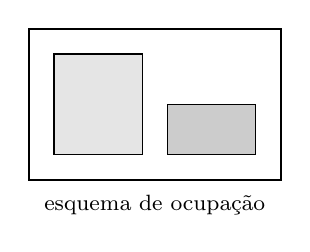
\begin{tikzpicture}[scale=0.8]
  \draw[thick] (0,0) rectangle (4,2.4);
  \draw[fill=gray!20] (0.4,0.4) rectangle (1.8,2);
  \draw[fill=gray!40] (2.2,0.4) rectangle (3.6,1.2);
  \node at (2,-0.4) {\footnotesize esquema de ocupação};
\end{tikzpicture}
\fonte{Elaboração própria.}
\end{mapa}

\begin{mapa}[ht]
\centering
\caption{Segundo mapa, para provar o contador e a lista}
\label{mapa:segundo}
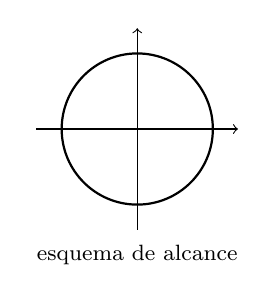
\begin{tikzpicture}[scale=0.8]
  \draw[thick] (0,0) circle (1.2);
  \draw[->] (-1.6,0) -- (1.6,0);
  \draw[->] (0,-1.6) -- (0,1.6);
  \node at (0,-2) {\footnotesize esquema de alcance};
\end{tikzpicture}
\fonte{Elaboração própria.}
\end{mapa}


\section{Tabelas mais elegantes}

Atualmente a tendência é usar tabelas mais leves, como \autoref{tab:exemplo_numerosbom}. Isso exige o pacote \verb*|booktabs|.

\begin{table}[ht]
\centering % Centraliza a tabela
\caption{Exemplo de Tabela de Números mais elegantes}
\label{tab:exemplo_numerosbom}
\begin{tabular}{ccc} % Define a quantidade de colunas
\toprule % Linha superior
\textbf{Col. 1} & \textbf{Col. 2} & \textbf{Col. 3} \\ % Cabeçalhos
\midrule % Linha média
1 & 2 & 3 \\ % Primeira linha de dados
4 & 5 & 6 \\ % Segunda linha de dados
7 & 8 & 9 \\ % Terceira linha de dados
10 & 11 & 12 \\ % Quarta linha de dados
\bottomrule % Linha inferior
\end{tabular}
\fonte{Elaboração própria.}
\end{table}

\section{Tabelas Longas ou Largas}

Se sua tabela é muito longa ou larga, existem várias opções.
\begin{itemize}
    \item alterar o tamanho da letra
    \item Usar o longtable
    \item rodar a tabela, fazendo ela em \textit{landscape}
    \item fazer a tabela dentro de um minibox
\end{itemize}


\subsection{Tabelas largas demais}

É comum em teses que as tabelas sejam largas demais. Há várias formas de resolver isso.

A \autoref{tab:tabela_largafns} é larga demais para a mancha, e o que se fez nela foi diminuir o corpo da fonte com o comando \verb|\footnotesize|, colocado dentro do ambiente \verb|table|, antes do \verb|tabular|.

\begin{table}[ht]
\centering % Centraliza a tabela
\caption{Exemplo de Tabela Larga com Fonte Menor}
\label{tab:tabela_largafns}
\footnotesize % Aplica uma fonte menor para a tabela
\begin{tabular}{cccccccc} % Aumente o número de colunas conforme necessário
\toprule
\textbf{Col. 1} & \textbf{Col. 2} & \textbf{Col. 3} & \textbf{Col. 4} & \textbf{Col. 5} & \textbf{Col. 6} & \textbf{Col. 7} & \textbf{Col. 8} \\
\midrule
Dado 1.1 & Dado 1.2 & Dado 1.3 & Dado 1.4 & Dado 1.5 & Dado 1.6 & Dado 1.7 & Dado 1.8 \\
Dado 2.1 & Dado 2.2 & Dado 2.3 & Dado 2.4 & Dado 2.5 & Dado 2.6 & Dado 2.7 & Dado 2.8 \\
Dado 3.1 & Dado 3.2 & Dado 3.3 & Dado 3.4 & Dado 3.5 & Dado 3.6 & Dado 3.7 & Dado 3.8 \\
\bottomrule
\end{tabular}
\fonte{Elaboração própria.}
\end{table}

O comando \verb|\resizebox{width}{height}{content}| permite ajustar o tamanho de qualquer coisa, inclusive uma tabela, como na \autoref{tab:examplerb}. No caso, estou fazendo a tabela ficar maior, para ocupar o espaço, mas funciona para qualquer tamanho.

\begin{table}[ht]
\centering
\caption{Exemplo de Tabela Redimensionada}
\label{tab:examplerb}
\resizebox{\textwidth}{!}{%
\begin{tabular}{llll}
\toprule
Coluna 1 & Coluna 2 & Coluna 3 & Coluna 4 \\
\midrule
Dados 1 & Dados 2 & Dados 3 & Dados 4 \\
Dados 5 & Dados 6 & Dados 7 & Dados 8 \\
\bottomrule
\end{tabular}%
}
\fonte{Elaboração própria.}
\end{table}


Para rodar uma tabela muito larga em 90 graus no LaTeX, você pode usar o pacote \verb*|rotating|. Este pacote fornece o ambiente \verb*|sidewaystable|, que automaticamente gira a tabela, incluindo sua legenda, em 90 graus. Isso é especialmente útil para acomodar tabelas largas em documentos, garantindo que elas caibam na página sem comprometer a legibilidade.

Aqui está um exemplo de como usar o ambiente \verb*|sidewaystable| para girar uma tabela. Primeiro, apresento o código dentro de um ambiente verbatim para mostrar como ele deve ser escrito no seu documento \LaTeX. Em seguida, forneço o mesmo código fora do ambiente verbatim para demonstrar como ele funcionaria na prática. A tabela aqui é pequena, só para ilustrar.

\begin{sidewaystable}
\centering
\caption{Sua Legenda Aqui}
\label{tab:sua_tabela}
\begin{tabular}{lll}
\toprule
Coluna 1 & Coluna 2 & Coluna 3 \\
\midrule
Item 1 & Item 2 & Item 3 \\
Item 4 & Item 5 & Item 6 \\
\bottomrule
\end{tabular}
\fonte{Elaboração própria.}
\end{sidewaystable}

Se a tabela for muito longa, o ambiente \verb|longtable| é o ideal. Ele fornece comandos para \textit{headers}, cabeçalhos, e \textit{footers} tanto no ínicio e no fim da tabela, como em todas as páginas. A \autoref{tab:longa} fornece um exemplo de 3 páginas.

% Exemplo de tabela longa que se estende por várias páginas
\begin{longtable}{|c|c|c|}
% primeiro cabeçalho (é o caption)
\caption{Exemplo de Tabela Longa}\label{tab:longa} \\
\hline \textbf{Col. 1} & \textbf{Col. 2} & \textbf{Col. 3} \\ \hline
\endfirsthead
% cabeçalho normal
\multicolumn{3}{c}%
{{\tablename\ \thetable{} -- continuação da página anterior}} \\
\hline \textbf{Col. 1} & \textbf{Col. 2} & \textbf{Col. 3} \\ \hline
\endhead
% pé normal
\hline \multicolumn{3}{|r|}{{Continua na próxima página}} \\ \hline
\endfoot
\hline
% último pé
\multicolumn{3}{|r|}{{Continua na próxima página}}\\
\hline \hline
\endlastfoot

% Conteúdo da tabela
1 & 2 & 3 \\
4 & 5 & 6 \\
1 & 2 & 3 \\
4 & 5 & 6 \\
1 & 2 & 3 \\
4 & 5 & 6 \\
1 & 2 & 3 \\
4 & 5 & 6 \\
1 & 2 & 3 \\
4 & 5 & 6 \\
1 & 2 & 3 \\
4 & 5 & 6 \\
1 & 2 & 3 \\
4 & 5 & 6 \\
1 & 2 & 3 \\
4 & 5 & 6 \\
1 & 2 & 3 \\
1 & 2 & 3 \\
4 & 5 & 6 \\
1 & 2 & 3 \\
4 & 5 & 6 \\
1 & 2 & 3 \\
4 & 5 & 6 \\
1 & 2 & 3 \\
4 & 5 & 6 \\
1 & 2 & 3 \\
4 & 5 & 6 \\
1 & 2 & 3 \\
4 & 5 & 6 \\
1 & 2 & 3 \\
4 & 5 & 6 \\
1 & 2 & 3 \\
4 & 5 & 6 \\
1 & 2 & 3 \\
4 & 5 & 6 \\
1 & 2 & 3 \\
4 & 5 & 6 \\
1 & 2 & 3 \\
4 & 5 & 6 \\
1 & 2 & 3 \\
4 & 5 & 6 \\1 & 2 & 3 \\
4 & 5 & 6 \\
1 & 2 & 3 \\
4 & 5 & 6 \\
1 & 2 & 3 \\
1 & 2 & 3 \\
4 & 5 & 6 \\
1 & 2 & 3 \\
4 & 5 & 6 \\
1 & 2 & 3 \\
4 & 5 & 6 \\
1 & 2 & 3 \\
4 & 5 & 6 \\
1 & 2 & 3 \\
4 & 5 & 6 \\
1 & 2 & 3 \\
4 & 5 & 6 \\
1 & 2 & 3 \\
4 & 5 & 6 \\
1 & 2 & 3 \\
4 & 5 & 6 \\
1 & 2 & 3 \\
4 & 5 & 6 \\
1 & 2 & 3 \\
4 & 5 & 6 \\
1 & 2 & 3 \\
4 & 5 & 6 \\
1 & 2 & 3 \\
4 & 5 & 6 \\
1 & 2 & 3 \\
4 & 5 & 6 \\
1 & 2 & 3 \\
4 & 5 & 6 \\
1 & 2 & 3 \\
4 & 5 & 6 \\
1 & 2 & 3 \\
4 & 5 & 6 \\
1 & 2 & 3 \\
4 & 5 & 6 \\
1 & 2 & 3 \\
4 & 5 & 6 \\
1 & 2 & 3 \\
4 & 5 & 6 \\
1 & 2 & 3 \\
4 & 5 & 6 \\
1 & 2 & 3 \\
4 & 5 & 6 \\
1 & 2 & 3 \\
4 & 5 & 6 \\
1 & 2 & 3 \\
4 & 5 & 6 \\
1 & 2 & 3 \\
4 & 5 & 6 \\
1 & 2 & 3 \\
4 & 5 & 6 \\
1 & 2 & 3 \\
4 & 5 & 6 \\
1 & 2 & 3 \\
4 & 5 & 6 \\
1 & 2 & 3 \\
4 & 5 & 6 \\
1 & 2 & 3 \\
4 & 5 & 6 \\
1 & 2 & 3 \\
4 & 5 & 6 \\
1 & 2 & 3 \\
4 & 5 & 6 \\

% Repetir linhas semelhantes conforme necessário para estender a tabela por 3 páginas
\end{longtable}
\fonte{Elaboração própria.}% a longtable não é float: a fonte vem após o ambiente

\section{Subfiguras (subcaption)}

Para colocar várias imagens (ou tabelas) lado a lado, cada uma com sua própria legenda, use o pacote \verb|subcaption|. \textbf{Evite} \verb|subfigure| e \verb|subfig|: são obsoletos e conflitam com a configuração de legendas. A \autoref{fig:subs} traz duas subfiguras:

\begin{figure}[ht]
  \centering
  \begin{subfigure}[b]{0.42\textwidth}
    \centering\includegraphics[width=\linewidth]{example-image-a}
    \caption{Primeira vista}\label{fig:sub-a}
  \end{subfigure}
  \hfill
  \begin{subfigure}[b]{0.42\textwidth}
    \centering\includegraphics[width=\linewidth]{example-image-b}
    \caption{Segunda vista}\label{fig:sub-b}
  \end{subfigure}
  \caption{Figura com duas subfiguras}
  \label{fig:subs}
  \fonte{Elaboração própria.}
\end{figure}

Referencie a figura inteira com \verb|\autoref{fig:subs}|. Cada parte tem
rótulo próprio: \verb|\autoref{fig:sub-a}| leva à \autoref{fig:sub-a}.

\section{Imagens (graphicx)}

A classe já carrega o \verb|graphicx|. Insira imagens com \verb|\includegraphics|; as opções mais úteis são:
\begin{itemize}
  \item \verb|[width=0.8\textwidth]| ou \verb|[scale=0.5]| --- tamanho;
  \item \verb|[angle=90]| --- rotação;
  \item \verb|[trim=l b r t, clip]| --- recorte (corta as bordas \emph{esquerda, baixo, direita, topo}).
\end{itemize}
Formatos aceitos com \hologo{pdfLaTeX}/\hologo{LuaLaTeX}: \texttt{pdf}, \texttt{png}, \texttt{jpg}. Arquivos \texttt{eps} são convertidos automaticamente (\texttt{epstopdf}). Imagens \texttt{svg} exigem um programa externo (ex.: Inkscape) ou o pacote \verb|svg| com \verb|--shell-escape|; o mais simples é exportar o \texttt{svg} para \texttt{pdf} antes de incluí-lo.

\section{Introdução ao tikz}

O \verb|tikz| (disponível também via \verb|tcolorbox|) desenha gráficos vetoriais no próprio \LaTeX: o desenho sai com a mesma fonte do texto, escala sem perder qualidade e não depende de arquivo externo. A \autoref{fig:tikz} é um fluxograma de três etapas, e o código dela está logo abaixo, comentado. Como toda ilustração, a legenda vai \textbf{acima} e a fonte \textbf{abaixo}.

\begin{figure}[ht]
  \centering
  \caption{Diagrama simples em tikz}
  \label{fig:tikz}
  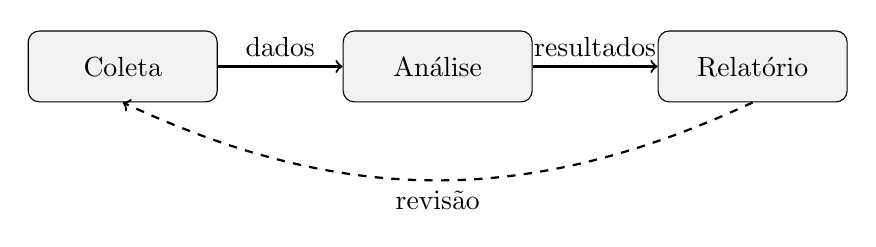
\begin{tikzpicture}[
      % um estilo com nome, para não repetir as mesmas opções em cada nó
      etapa/.style={draw, rounded corners, minimum width=2.4cm,
                    minimum height=0.9cm, fill=gray!10},
      seta/.style={->, thick}]
    % os nós: estilo, nome entre parênteses, posição (x,y) em cm, texto
    \node[etapa] (coleta)  at (0,0) {Coleta};
    \node[etapa] (analise) at (4,0) {Análise};
    \node[etapa] (relato)  at (8,0) {Relatório};
    % as setas ligam os nós pelo nome; o rótulo vai no meio, por cima
    \draw[seta] (coleta)  -- (analise) node[midway, above] {dados};
    \draw[seta] (analise) -- (relato)  node[midway, above] {resultados};
    % uma seta de volta, curvada por baixo
    \draw[seta, dashed] (relato.south) to[bend left=25]
      node[midway, below] {revisão} (coleta.south);
  \end{tikzpicture}
  \fonte{Elaboração própria.}
\end{figure}

\begin{verbatim}
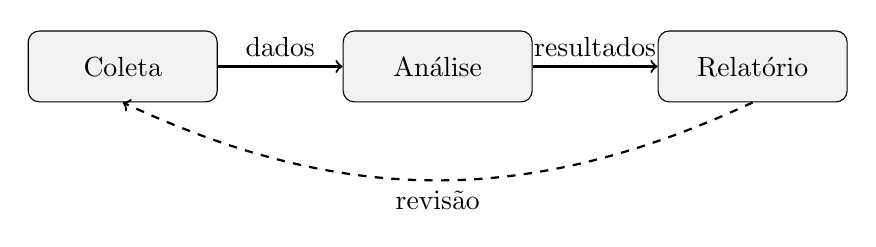
\begin{tikzpicture}[
    etapa/.style={draw, rounded corners, minimum width=2.4cm,
                  minimum height=0.9cm, fill=gray!10},
    seta/.style={->, thick}]
  \node[etapa] (coleta)  at (0,0) {Coleta};
  \node[etapa] (analise) at (4,0) {Análise};
  \node[etapa] (relato)  at (8,0) {Relatório};
  \draw[seta] (coleta)  -- (analise) node[midway, above] {dados};
  \draw[seta] (analise) -- (relato)  node[midway, above] {resultados};
  \draw[seta, dashed] (relato.south) to[bend left=25]
    node[midway, below] {revisão} (coleta.south);
\end{tikzpicture}
\end{verbatim}

Três ideias bastam para começar: \textbf{nós} (\verb|\node|) são caixas de texto com nome e posição; \textbf{caminhos} (\verb|\draw|) ligam coordenadas ou nós; e \textbf{estilos} (\verb|nome/.style|) guardam opções para reaproveitar. Para gráficos de dados (curvas, barras), veja o \verb|pgfplots|, construído sobre o \verb|tikz|. A documentação do \verb|tikz| (\texttt{texdoc tikz}) começa com tutoriais.

\section{Float ou direto no texto?}

Colocar a tabela ou imagem dentro de \verb|figure|/\verb|table| (um \emph{float}) deixa o \LaTeX\ posicioná-la onde melhor couber (topo ou base da página), numerá-la e incluí-la na lista; em troca, a posição exata não é garantida. Colocá-la \emph{diretamente} no texto fixa a posição, mas perde a numeração, a legenda e a entrada na lista, além de poder gerar quebras de página ruins. Para teses, prefira sempre o float, com \verb|\caption| e \verb|\source|.

  \chapter{Using BibLaTeX}
  \label{cap:biblatex}

  Esta classe gera as referências com BibLaTeX e o \emph{backend} \texttt{biber}, no padrão ABNT (NBR~6023 para as referências e NBR~10520 para as citações), seguindo as normas da CPGP da COPPE. O antigo \hologo{BibTeX} e os arquivos \texttt{.bst} foram aposentados.

  \textbf{É obrigatório compilar com \texttt{biber}} (e não com \hologo{BibTeX}). A sequência de compilação é: \hologo{LaTeX}, depois \texttt{biber}, e mais duas vezes \hologo{LaTeX}. Em editores como o \hologo{TeX}studio ou o Overleaf, configure o \emph{bibliography backend} como \texttt{biber} (veja o capítulo sobre \texttt{latexmkrc}).

  Os comandos do \texttt{natbib} (\verb|\citet|, \verb|\citep|) continuam disponíveis porque a classe carrega o BibLaTeX com a opção \texttt{natbib=true}; assim, você pode usar tanto os comandos nativos do BibLaTeX (\verb|\autocite|, \verb|\textcite|) quanto os do \texttt{natbib}. As Tabelas~\ref{tab:citation} e~\ref{tab:citation1} apresentam \verb|\cite| e \verb|\citet| para vários tipos de obra contidos na norma da CPGP (a primeira com regras manuais, a segunda com \texttt{booktabs}), no estilo numérico. Tirando o parâmetro opcional numérico da classe, as citações passam de numéricas para autor-data.

  \begin{table}[htb]
  \caption{Exemplos de citações utilizando o comando padrão
    \texttt{\textbackslash cite} do \LaTeX\ e
    o comando \texttt{\textbackslash citep},
    disponível pela opção \texttt{natbib} do BibLaTeX.}
  \label{tab:citation}
  \centering
  {\footnotesize
  \begin{tabular}{|c|c|c|}
    \hline
    Tipo da Publicação & \verb|\cite| & \verb|\citep|\\
    \hline
    Livro & \cite{book-example} & \citep{book-example}\\
    Artigo & \cite{article-example} & \citep{article-example}\\
    Relatório & \cite{techreport-example} & \citep{techreport-example}\\
    Relatório & \cite{techreport-exampleIn} & \citep{techreport-exampleIn}\\
    Anais de Congresso & \cite{inproceedings-example} &
      \citep{inproceedings-example}\\
    Séries & \cite{incollection-example} & \citep{incollection-example}\\
    Em Livro & \cite{inbook-example} & \citep{inbook-example}\\
    Dissertação de mestrado & \cite{mastersthesis-example} &
      \citep{mastersthesis-example}\\
    Tese de doutorado & \cite{phdthesis-example} & \citep{phdthesis-example}\\
    \hline
  \end{tabular}}
  \fonte{Elaboração própria.}
  \end{table}

 \begin{table}[htb]
  \caption{Exemplos de citações utilizando o comando padrão
    \texttt{\textbackslash cite} do \LaTeX\ e
    o comando \texttt{\textbackslash citet},
    disponível pela opção \texttt{natbib} do BibLaTeX. Além disso, usando o booktabs.}
  \label{tab:citation1}
  \centering
  {\footnotesize
  \begin{tabular}{ccc}
    \toprule
    Tipo da Publicação & \verb|\cite| & \verb|\citet|\\
    \midrule
    Livro & \cite{book-example} & \citet{book-example}\\
    Artigo & \cite{article-example} & \citet{article-example}\\
    Relatório & \cite{techreport-example} & \citet{techreport-example}\\
    Relatório & \cite{techreport-exampleIn} & \citet{techreport-exampleIn}\\
    Anais de Congresso & \cite{inproceedings-example} &
      \citet{inproceedings-example}\\
    Séries & \cite{incollection-example} & \citet{incollection-example}\\
    Em Livro & \cite{inbook-example} & \citet{inbook-example}\\
    Dissertação de mestrado & \cite{mastersthesis-example} &
      \citet{mastersthesis-example}\\
    Tese de doutorado & \cite{phdthesis-example} & \citet{phdthesis-example}\\
    \bottomrule
  \end{tabular}}
  \fonte{Elaboração própria.}
  \end{table}

  \section{Comandos de citação}

  Os principais comandos são: \verb|\cite| (referência simples), \verb|\citet| (autor por extenso, ano entre parênteses --- ``citação no texto''), \verb|\citep| (tudo entre parênteses) e os nativos do BibLaTeX \verb|\autocite| e \verb|\textcite|. Por exemplo, \citet{article-example} tratou do tema, o que também aparece em \citep{article-example}.

  \subsection{Parâmetro opcional: página e ``tradução nossa''}

  Todos os comandos aceitam um parâmetro opcional para a localização (página, seção) e observações. Por exemplo, \verb|\citep[p.~45, tradução nossa]{chave}| produz \citep[p.~45, tradução nossa]{article-example}. Use ``tradução nossa'' quando você mesmo traduziu o trecho citado (NBR~10520): coloque a tradução no corpo do texto e, se a precisão lexical importar, o original em nota de rodapé.

  \subsection{Citação de citação (\emph{apud})}

  Para citar uma obra através de outra, use \verb|\citetapud| e \verb|\citepapud| (demonstrados na Seção~\ref{sec:citacoes}): pela ABNT, entra na lista de referências \emph{apenas} a obra efetivamente consultada; a obra original (não consultada) é informada como texto.

  \subsection{Múltiplas bibliografias}

  Para separar as referências (por tipo, capítulo ou tema), use o ambiente \verb|refsection| e vários \verb|\printbibliography| com filtros, como \verb|\printbibliography[type=article]| ou \verb|\printbibliography[keyword=lei]|. Cada chamada imprime um subconjunto das entradas citadas.

  \section{Tipos de entrada bibliográfica}

  Cada tipo de documento da ABNT corresponde a um tipo de entrada do BibLaTeX, com um sinônimo em português (sem acentos) que você pode usar no \texttt{.bib}. Todos os tipos abaixo estão demonstrados nas Referências deste documento (veja \texttt{example.bib}). Entre parênteses, os sinônimos em português.

  % Nomes de tipo em fonte de máquina não hifenizam: justificados, abriam
  % buracos nas linhas (Underfull \hbox). Alinhado à esquerda, não.
  \begingroup\raggedright
  \subsection{Tipos acadêmicos principais}
  \begin{itemize}
    \item Livro / monografia --- \verb|@book| (\verb|@livro|)
    \item Artigo de periódico --- \verb|@article| (\verb|@artigo|); matéria de jornal --- \verb|@article| (\verb|@artigodejornal|)
    \item Capítulo de livro --- \verb|@incollection| (\verb|@partedelivro|), \verb|@inbook| (\verb|@emlivro|); verbete --- \verb|@inreference| (\verb|@verbete|)
    \item Evento no todo (anais) --- \verb|@proceedings| (\verb|@anais|); trabalho em evento --- \verb|@inproceedings| (\verb|@trabalhodeevento|)
    \item Tese/dissertação --- \verb|@thesis| (\verb|@tese|, \verb|@dissertacao|); com tipo predefinido: \verb|@dissertacaomestrado|, \verb|@tesedoutorado|, \verb|@tesephd|, \verb|@tcc|
    \item Relatório --- \verb|@report| (\verb|@relatorio|, \verb|@relatoriotecnico|); periódico no todo --- \verb|@periodical| (\verb|@periodico|)
    \item Manual --- \verb|@manual|; diversos --- \verb|@misc| (\verb|@diverso|); página/site --- \verb|@online|
  \end{itemize}

  \subsection{Tipos especiais (ABNT §4.2.5--4.2.14)}
  \begin{itemize}
    \item Patente --- \verb|@patent| (\verb|@patente|)
    \item Legislação / ato normativo --- \verb|@legislation| (\verb|@legislacao|, \verb|@atonormativo|); jurisprudência --- \verb|@jurisdiction| (\verb|@jurisprudencia|); documento jurídico/civil --- \verb|@legal| (\verb|@documentojuridico|, \verb|@documentocivil|)
    \item Norma técnica --- \verb|@standard| (\verb|@norma|); partitura --- \verb|@music| (\verb|@partitura|)
    \item Documento cartográfico (mapa) --- \verb|@map| (\verb|@mapa|, \verb|@cartografico|); iconográfico --- \verb|@image| (\verb|@iconografico|); obra de arte/3D --- \verb|@artwork| (\verb|@obradearte|, \verb|@tridimensional|)
    \item Audiovisual --- \verb|@video| (\verb|@audiovisual|); filme --- \verb|@movie| (\verb|@filme|); correspondência --- \verb|@letter| (\verb|@correspondencia|); conjunto de dados --- \verb|@dataset| (\verb|@conjuntodedados|)
  \end{itemize}

  \subsection{Jogos e TV (tipos próprios da CoppeTeX)}
  \begin{itemize}
    \item Jogo --- \verb|@game| (\verb|@jogo|); de tabuleiro --- \verb|@boardgame| (\verb|@jogodetabuleiro|); eletrônico --- \verb|@videogame| (\verb|@jogoeletronico|)
    \item Programa de TV / série --- \verb|@tvshow| (\verb|@programadetv|, \verb|@serietv|)
  \end{itemize}

  Os campos também aceitam sinônimos em português (sem acentos): \verb|autor|, \verb|titulo|, \verb|subtitulo|, \verb|editora|, \verb|local|, \verb|ano|, \verb|data|, \verb|paginas|, \verb|edicao|, \verb|numero|, \verb|periodico|/\verb|jornal|/\verb|revista|, \verb|caderno|, \verb|escala|, \verb|organizador|, \verb|tradutor|, entre outros. Sem autor nem organizador, a entrada é feita pelo título, com a 1ª palavra em CAIXA ALTA.
  \par\endgroup

  \section{Uma referência de cada categoria do Manual}\label{sec:todosostipos}

  A seção 4.2 do Manual do SiBI enumera 34 categorias de documento, da monografia à partitura. O arquivo \verb|tipos.bib|, que acompanha a classe, traz \textbf{uma entrada de cada uma}, com os dados dos próprios exemplos do Manual, e todas são citadas aqui. Confira cada uma na lista de Referências: é assim que ela tem de sair.

  Metade das entradas está escrita com os nomes de tipo e de campo em \textbf{inglês} e metade com os sinônimos em \textbf{português}, de propósito, para que as duas formas apareçam funcionando lado a lado. \textbf{Prefira a inglesa}: é a do \texttt{biblatex}, é a que os gerenciadores de referência exportam, e é a que outra pessoa vai reconhecer quatro anos depois. Os sinônimos em português existem para quem chega de uma base antiga e não quer reescrever tudo.

  % Colunas estreitas alinhadas à esquerda: justificadas, abriam buracos.
  \begin{longtable}{@{}>{\raggedright\arraybackslash}p{0.46\textwidth}>{\raggedright\arraybackslash}p{0.17\textwidth}>{\raggedright\arraybackslash}p{0.28\textwidth}@{}}
    \caption{Uma referência de cada categoria da seção 4.2 do Manual}
    \label{tab:todosostipos}\\
    \toprule
    \textbf{Categoria} & \textbf{Forma usada} & \textbf{Citação} \\
    \midrule
    \endfirsthead
    \toprule
    \textbf{Categoria} & \textbf{Forma usada} & \textbf{Citação} \\
    \midrule
    \endhead
    \bottomrule
    \endfoot
    4.2.1.1 monografia no todo & inglesa & \cite{m-4211} \\
    4.2.1.2 monografia em meio eletrônico & portuguesa & \cite{m-4212} \\
    4.2.1.3 parte de monografia & inglesa & \cite{m-4213} \\
    4.2.2 correspondência & portuguesa & \cite{m-422} \\
    4.2.2.1 correspondência em meio eletrônico & inglesa & \cite{m-4221} \\
    4.2.3.1 publicação periódica no todo & portuguesa & \cite{m-4231} \\
    4.2.3.3 parte de revista & inglesa & \cite{m-4233} \\
    4.2.3.4 artigo de revista & portuguesa & \cite{m-4234} \\
    4.2.3.5 artigo de revista em meio eletrônico & inglesa & \cite{m-4235} \\
    4.2.3.6 matéria de jornal & portuguesa & \cite{m-4236} \\
    4.2.3.7 matéria de jornal assinada, em meio eletrônico & inglesa & \cite{m-4237} \\
    4.2.3.8 matéria de jornal não assinada, em meio eletrônico & portuguesa & \cite{m-4238} \\
    4.2.4.1 evento no todo & inglesa & \cite{m-4241} \\
    4.2.4.3 evento no todo em meio eletrônico & portuguesa & \cite{m-4243} \\
    4.2.4.5 trabalho apresentado em evento & inglesa & \cite{m-4245} \\
    4.2.4.6 trabalho em evento, em meio eletrônico & portuguesa & \cite{m-4246} \\
    4.2.5 patente & inglesa & \cite{m-425} \\
    4.2.5.1 patente em meio eletrônico & portuguesa & \cite{m-4251} \\
    4.2.6.1 legislação & inglesa & \cite{m-4261} \\
    4.2.6.2 jurisprudência & portuguesa & \cite{m-4262} \\
    4.2.6.3 ato administrativo normativo & inglesa & \cite{m-4263} \\
    4.2.7 documento jurídico em meio eletrônico & portuguesa & \cite{m-427} \\
    4.2.8 documento civil e de cartório & inglesa & \cite{m-428} \\
    4.2.9 documento audiovisual & portuguesa & \cite{m-429} \\
    4.2.10 partitura & inglesa & \cite{m-42101} \\
    4.2.10.1 partitura em meio eletrônico & portuguesa & \cite{m-42102} \\
    4.2.11 documento iconográfico & inglesa & \cite{m-42111} \\
    4.2.11.1 documento iconográfico em meio eletrônico & portuguesa & \cite{m-42112} \\
    4.2.12 documento cartográfico & inglesa & \cite{m-42121} \\
    4.2.12.1 documento cartográfico em meio eletrônico & portuguesa & \cite{m-42122} \\
    4.2.13 documento tridimensional & inglesa & \cite{m-42131} \\
    4.2.14 documento de acesso exclusivo em meio eletrônico & portuguesa & \cite{m-4214} \\
    dissertação de mestrado & inglesa & \cite{m-diss} \\
    norma técnica & portuguesa & \cite{m-norma} \\
  \end{longtable}
  \fonte{Elaboração própria, a partir da seção 4.2 do Manual do SiBI.}

  Se alguma dessas referências sair diferente do que o Manual imprime, é defeito da classe, e o lugar de relatar é o repositório do projeto. O gabarito de cada uma está no próprio \verb|tipos.bib|, em comentário acima da entrada.

\chapter{Alguns outros exemplo úteis}

\begin{tcolorbox}[title=Meu Textbox]
Este é o conteúdo do meu textbox. Você pode adicionar qualquer texto aqui, bem como incluir fórmulas matemáticas, listas e outros elementos que desejar. A caixa ajustará automaticamente o tamanho para acomodar seu conteúdo.
\end{tcolorbox}

\begin{tcolorbox}
Este é o conteúdo do meu textbox sem título. Você pode adicionar qualquer texto aqui, bem como incluir fórmulas matemáticas, listas e outros elementos que desejar. A caixa ajustará automaticamente o tamanho para acomodar seu conteúdo.
\end{tcolorbox}

\begin{figure}[ht]
    \centering
    \begin{tikzpicture}
        \node[anchor=south west,inner sep=0] (image) at (0,0) {\includegraphics[width=0.5\textwidth]{example-image}}; % Substitua example-image pelo nome da sua imagem
        \begin{scope}[x={(image.south east)},y={(image.north west)}]
            % Definindo o textbox dentro da figura
            \node[anchor=north west, text width=0.3\textwidth, fill=white, opacity=0.7, text opacity=1] at (0.05,0.95) { % Ajuste a posição conforme necessário
                \begin{tcolorbox}[colback=red!5!white,colframe=red!75!black,halign=flush left,halign title=flush left,title=Textbox dentro de uma figura]
                    Este textbox fala sobre como inserir um textbox dentro de uma figura usando o pacote \texttt{tikz} e \texttt{tcolorbox} no \LaTeX.
                \end{tcolorbox}
            };
        \end{scope}
    \end{tikzpicture}
    \caption{Figura com Textbox}
    \label{fig:figura_com_textbox1}
    \fonte{Elaboração própria.}
\end{figure}


\begin{figure}[ht]
    \centering
 \begin{tcolorbox}
Este é o conteúdo do meu textbox sem título. Você pode adicionar qualquer texto aqui, bem como incluir fórmulas matemáticas, listas e outros elementos que desejar. A caixa ajustará automaticamente o tamanho para acomodar seu conteúdo. O textbox agora foi posto dentro de uma figura.
\end{tcolorbox}
    \caption{Figura com Textbox simples}
    \label{fig:figura_com_textbox}
    \fonte{Elaboração própria.}
\end{figure}

\section{Listagens de código e algoritmos}

O CoppeTeX traz embutido o suporte a listagens de programas (pacote \verb|listings|) e a algoritmos (\verb|algorithm2e|). A legenda fica no topo (``Programa N''), como em qualquer ilustração, e a lista correspondente é gerada por \verb|\listofprogramas|. O \autoref{prog:exemplo} mostra um exemplo em Python.

\begin{python}[caption={Exemplo de programa em Python},label=prog:exemplo]
def saudacao(nome):
    # imprime uma saudação acentuada
    print(f"Olá, {nome}!")

saudacao("COPPE")
\end{python}
\source{Elaboração própria.}

Para inserir código no meio do texto use \verb|\pythoninline|, como em \pythoninline{saudacao(nome)}; e para mostrar a saída de um programa use o ambiente \verb|Verbatim| do \texttt{fancyvrb}, que a classe já carrega:

\begin{Verbatim}[frame=lines,numbers=left,numbersep=0.5em]
Olá, COPPE!
\end{Verbatim}

Há estilos prontos também para \verb|java|, \verb|xml|, \verb|html| e \verb|prolog|. O \autoref{prog:java} usa o de Java e é a segunda listagem do documento, o que prova que o contador anda e que as duas entram na lista de programas.

\begin{java}[caption={Exemplo de programa em Java},label=prog:java]
public class Saudacao {
    public static void main(String[] args) {
        System.out.println("Olá, COPPE!");
    }
}
\end{java}
\fonte{Elaboração própria.}

Há também \verb|\pythoninline| e \verb|\javainline| para código no meio do
texto, como em \javainline{new Saudacao()}, e o ambiente \verb|Verbatim| (com as opções acima) para a saída de programas. Para algoritmos, use o ambiente \verb|algorithm| com as palavras-chave em português \verb|\Para| e \verb|\Enquanto|, como no \autoref{alg:soma}.

\begin{algorithm}[H]
\caption{Soma dos elementos de um vetor}
\label{alg:soma}
\Dados{vetor $v$ com $n$ elementos}
\Resultado{soma $s$ dos elementos de $v$}
$s \leftarrow 0$\;
\Para{$i \leftarrow 1$ \Ate{} $n$}{
  $s \leftarrow s + v[i]$\;
}
\Retorna $s$\;
\end{algorithm}

O \autoref{alg:busca} é o segundo algoritmo, e usa \verb|\Enquanto|. Como no caso das listagens, ele existe para mostrar a numeração andando e a lista de algoritmos com duas entradas.

\begin{algorithm}[H]
\caption{Busca sequencial em um vetor}
\label{alg:busca}
\Dados{vetor $v$ com $n$ elementos e uma chave $k$}
\Resultado{posição de $k$ em $v$, ou $0$ se $k$ não estiver em $v$}
$i \leftarrow 1$\;
\Enquanto{$i \leq n$ \textbf{e} $v[i] \neq k$}{
  $i \leftarrow i + 1$\;
}
\Se{$i > n$}{\Retorna $0$\;}
\Retorna $i$\;
\end{algorithm}

  \chapter{Escrevendo matemática}

  A classe carrega \texttt{amsmath} em qualquer motor: são os ambientes e comandos, não a fonte. \textbf{A fonte matemática é escolha sua}, e a classe não carrega nenhuma. Este exemplo a escolhe no preâmbulo, pelo motor: \texttt{amssymb} sob \hologo{pdfLaTeX} (símbolos clássicos $\mathbb{R}$, $\hbar$, $\varnothing$, \ldots) e \texttt{unicode-math} com a Latin Modern Math sob \hologo{LuaLaTeX}/\hologo{XeLaTeX} (veja a~\autoref{sec:unicode-math}). Copie o bloco para o seu trabalho, troque a fonte se quiser, ou apague-o se o trabalho não tem matemática. Fórmulas no texto vão entre \verb|$...$|; fórmulas destacadas e numeradas usam o ambiente \verb|equation|.

  \section{Alinhamento (align)}
  O ambiente \verb|align| alinha equações pelo \verb|&| e numera cada linha (\verb|\\| quebra a linha; \verb|align*| não numera):
  \begin{align}
    f(x) &= (x+1)^2 \\
         &= x^2 + 2x + 1 .
  \end{align}

  \section{Matrizes (matrix)}
  O \texttt{amsmath} traz \verb|pmatrix|, \verb|bmatrix|, \verb|vmatrix|, entre outros:
  \begin{equation}
    A = \begin{bmatrix} a_{11} & a_{12} \\ a_{21} & a_{22} \end{bmatrix}
    \qquad
    \det A = \begin{vmatrix} a_{11} & a_{12} \\ a_{21} & a_{22} \end{vmatrix}
  \end{equation}

  \section{Subequações (subequations)}
  Para numerar um grupo de equações sob o mesmo número, com letras (a), (b):
  \begin{subequations}
  \begin{align}
    a &= b + c , \\
    d &= e - f .
  \end{align}
  \end{subequations}

  \section{Estruturas alinhadas (array)}
  O \verb|array| monta estruturas dentro do modo matemático, como definições por partes:
  \begin{equation}
    |x| = \left\{ \begin{array}{ll}
      x,  & \text{se } x \ge 0 , \\
      -x, & \text{caso contrário.}
    \end{array} \right.
  \end{equation}

  \section{Operadores (\textbackslash DeclareMathOperator)}
  Para operadores com a tipografia correta (romano, espaçamento adequado), declare-os no preâmbulo:
  \begin{verbatim}
  \usepackage{amsmath}
  \DeclareMathOperator{\RMSE}{RMSE}
  \DeclareMathOperator{\diag}{diag}
  \end{verbatim}
  Assim:
  \begin{itemize}
    \item \verb|$\RMSE(y,\hat{y})$| produz $\RMSE(y,\hat{y})$;
    \item \verb|$\diag(\lambda_1,\lambda_2)$| produz
          $\diag(\lambda_1,\lambda_2)$.
  \end{itemize}

  \section{Unicode e LuaLaTeX (unicode-math)}
  \label{sec:unicode-math}
  Ao migrar para \hologo{LuaLaTeX} (ou \hologo{XeLaTeX}), \textbf{não carregue} \texttt{amssymb}: ele é o pacote AMS legado, escrito para as fontes Type~1 de 8~bits (\texttt{msam}/\texttt{msbm}), e colide com \texttt{unicode-math} -- o pacote moderno que controla a fonte matemática OpenType. Por isso o preâmbulo deste exemplo escolhe um ou outro pelo motor, com \verb|\ifPDFTeX| (do pacote \texttt{iftex}, que a classe já carrega):
  \begin{verbatim}
  \ifPDFTeX
    \usepackage{amssymb}
  \else
    \usepackage{unicode-math} % NÃO use \usepackage{amssymb} junto
    \setmathfont{Latin Modern Math}  % ou STIX Two Math
  \fi
  \end{verbatim}
  O código clássico continua valendo ($\mathbb{R}$, $\int_a^b f(x)\,dx$, $\alpha$) e você ainda pode digitar os próprios símbolos Unicode no editor. A vantagem é que o PDF passa a indexar os símbolos em Unicode real: ao copiar uma fórmula do PDF, o significado dos símbolos é preservado.

  \chapter{Referências cruzadas, notas e índices}
  \label{cap:refs}

  Este capítulo reúne os recursos para \emph{apontar} para coisas: rótulos, notas de rodapé, hyperlinks, URLs e índices. (Para a bibliografia, veja o Capítulo~\ref{cap:biblatex}.)

  \section{Rótulos e referências cruzadas}

  Marque um elemento com \verb|\label{tipo:nome}| e aponte para ele com \verb|\ref| (só o número), \verb|\autoref| (tipo + número, p.\,ex.\ ``Figura 4.1'') ou \verb|\pageref| (a página). O número vem do contador do elemento \emph{no momento} do \verb|\label|; por isso o \verb|\label| deve vir logo após o \verb|\caption| (em floats) ou o título da seção. Adote prefixos por tipo: \verb|cap:|, \verb|sec:|, \verb|fig:|, \verb|tab:|, \verb|eq:|. Por exemplo, este é o \autoref{cap:refs} e a \autoref{fig:tikz} está no capítulo de floats.

  \section{Notas de rodapé}

  Use \verb|\footnote{texto}|\footnote{Como esta nota, que a classe imprime em espaçamento simples.}. Para repetir a marca sem renumerar, use \verb|\footnotemark| e \verb|\footnotetext|.

  \section{hyperref e marcadores}

  A classe carrega o \verb|hyperref|: o sumário, as citações e os \verb|\ref|/\verb|\autoref| viram \emph{links} clicáveis e o leitor de PDF ganha um painel de \emph{bookmarks} (navegação por capítulos). Não é preciso configurar nada; para mudar a cor dos links, use \verb|\hypersetup{...}| no preâmbulo. Para tirar a cor e a moldura de todos eles de uma vez --- útil para quem vai imprimir --- passe a opção de classe \verb|semlinks|; os links continuam clicáveis e os \emph{bookmarks} continuam no painel.

  \section{URLs}

  Para endereços, use \verb|\url{https://exemplo.org}|: o \verb|hyperref| cria o link e quebra a URL no fim da linha. Para um texto-âncora,
use \verb|\href{https://exemplo.org}{texto}|. Evite digitar URLs como texto comum --- elas não quebram e estouram a margem.

  \section{Índice remissivo}

  Marque os termos com \verb|\index{termo}| e imprima o índice com \verb|\printindex| (carregue \verb|makeidx| e use \verb|\makeindex| no preâmbulo). O índice é montado pelo programa \verb|makeindex|. Como as listas de abreviaturas e símbolos também usam \verb|makeindex| (com o estilo \verb|coppe.ist|), o mais prático é deixar o \verb|latexmk| rodar tudo (veja o \texttt{latexmkrc}). Atenção: o \verb|latexmk| é um script \emph{Perl} --- no Windows, instale o \emph{Strawberry Perl}; no Linux e no macOS o Perl já costuma vir instalado. Para vários índices, use \verb|imakeidx| ou \verb|index|.

  \section{Traduções (NBR 10520)}

  Ao citar um trecho que você mesmo traduziu, coloque a tradução no corpo do texto e escreva ``tradução nossa'' na chamada; se a precisão do original importar, ponha-o em nota de rodapé. Segundo \citet[p.~45]{article-example}, a interpretação depende das práticas (tradução nossa).\footnote{Original: ``the interpretation depends on the practices''.} Veja também o parâmetro opcional de \verb|\citep| no Capítulo~\ref{cap:biblatex}.

  \chapter{Truques de \LaTeX}

  \section{Comentários mágicos (\texttt{\% !TeX})}
  Linhas \verb|% !TeX| no topo do arquivo dizem ao editor (\hologo{TeX}studio, Overleaf, \hologo{TeX}works) como compilar. O padrão recomendado nesta classe:
  \begin{verbatim}
  % !TeX program = lualatex
  % !TeX encoding = UTF-8
  % !TeX spellcheck = pt_BR
  % !BIB program = biber
  \end{verbatim}
  Com isso o documento compila igual em qualquer ambiente. O \texttt{latexmkrc} cumpre papel parecido para o \verb|latexmk|.

  \section{Espaço engolido}
  Um comando sem argumento engole o espaço seguinte: \verb|\LaTeX é bom| sai como ``\LaTeX é bom'' (coladinho). Para preservar o espaço use \verb|\LaTeX\ é| (barra-espaço), \verb|\LaTeX{} é| (chaves vazias) ou o pacote \verb|xspace| ao definir o comando (\verb|\newcommand\foo{...\xspace}|).

  \section{Escopo (grupos)}
  Chaves \verb|{...}| (ou \verb|\begingroup|\dots\verb|\endgroup|) criam um escopo: mudanças de fonte, espaçamento e até definições de pacotes ficam locais. Para reaproveitar um pseudocódigo escrito para um pacote de algoritmos diferente do seu, isole-o num grupo em vez de reescrevê-lo.

  \section{Descarregar figuras: \texttt{\textbackslash clearpage} × \texttt{\textbackslash newpage}}
  \verb|\newpage| apenas quebra a página e leva os floats pendentes adiante, acumulando-os. \verb|\clearpage| quebra a página \emph{e} despeja todos os floats em espera antes de continuar --- use-o para evitar o ``congestionamento'' de figuras no fim de um capítulo.

  \section{\texttt{latexmkrc}, perl e Overleaf}
  O \verb|latexmk| automatiza a compilação (roda \LaTeX, \verb|biber| e \verb|makeindex| quantas vezes for preciso) e lê o \texttt{latexmkrc} do diretório. Como o \verb|latexmk| é um script \emph{Perl}, no Windows instale o \emph{Strawberry Perl}; no Linux e no macOS o Perl já vem instalado. No Overleaf, o \verb|latexmk| roda sozinho e lê o \texttt{latexmkrc} do projeto.

  \section{Fluxos de escrita e o \texttt{morewrites}}
  \label{sec:morewrites}

  O \hologo{pdfLaTeX} só consegue manter \textbf{dezesseis} arquivos abertos para escrita ao mesmo tempo, e cada lista que o trabalho imprime ocupa um deles até o fim da compilação: o sumário, a lista de figuras, a de tabelas, a de quadros, a de programas, a de algoritmos, cada flutuante novo criado com \verb|\newcoppefloat|, a lista de símbolos, a de abreviaturas, a de siglas, o índice remissivo, cada índice a mais e o glossário. Este exemplo, sozinho, passa dos dezesseis.

  Por isso a classe carrega o pacote \verb|morewrites|, que tira esse teto. Ele custa cerca de meio segundo por passada do \hologo{pdfLaTeX}. Quando o tempo de compilação importa --- no plano gratuito do Overleaf, por exemplo ---, a opção \verb|semmorewrites| o desliga:
  \begin{verbatim}
  \documentclass[dsc,semmorewrites]{coppe}
  \end{verbatim}

  \begin{itemize}
    \item \textbf{Pode desligar} se o trabalho \emph{não} tem índice remissivo, nem vários índices (\verb|imakeidx|, \verb|splitidx|), nem glossário, nem nomenclatura, e tem menos listas que este exemplo, que já precisa do pacote.
    \item \textbf{Deve desligar} se o \verb|morewrites| brigar com outro pacote, o que é raro: ele guarda o que é escrito até a página sair, e um pacote que escreve um arquivo e o lê de volta na mesma passada pode se perder.
    \item \textbf{Não desligue} se o trabalho tem índice remissivo e glossário, ou vários índices: é para isso que o pacote está ali.
  \end{itemize}

  Se você desligar e os fluxos acabarem, a compilação para com a mensagem ``Acabaram os 16 fluxos de escrita do \TeX'', que diz o que fazer: tirar o \verb|semmorewrites| ou compilar com \hologo{LuaLaTeX}, que tem cento e vinte e oito fluxos e dispensa o pacote. O manual da classe discute o assunto em detalhe, com o custo de cada lista.

  \chapter{Método Proposto}
  \chapter{Resultados e Discussões}

  \section{Algumas Demonstrações}

  A Lista de Símbolos sai na ordem em que cada símbolo aparece pela primeira vez no texto, como pede a seção 3.1.2.2.7 do Manual. Aqui vamos usar os símbolos $\alpha$ e $\beta$. A chave entre colchetes só vale com a opção de classe \verb|simbolosalfabeticos|, que ordena a lista alfabeticamente; sem ela, é ignorada.
  \symbl[beta]{Beta}{A palavra Beta more e corrigida}
  \symbl[zzbeta]{$\beta$}{A letra $\beta$ corrigida}
  \symbl{beta}{A palavra beta}
  \symbl{alpha}{A palavra alpha}
  \symbl[alpha]{Alpha}{A palavra Alpha}
  \symbl[zzalpha]{$\alpha$}{A letra $\alpha$ corrigida}
  \symbl[marco]{Marco}{A palavra Marco corrigida}

  A Lista de Abreviaturas é alfabética, e nela a chave entre colchetes decide a posição de siglas de caixa mista. Alguns exemplos:
  \abbrev{GoT}{Game of Thrones}
  \abbrev[GOT]{GoT}{Game of Thrones ordenado como GOT}
  \abbrev[iot]{IoT}{IoT ordenado como iot}
  \abbrev[IoT]{IoT}{IoT ordenado como IoT}
  \abbrev[IOT]{IoT}{IoT ordenado como IOT}
  \abbrev{IoT}{IoT com ordenação default}
  \abbrev[ITU]{ITU}{ITU mesmo}

  \newsigla{ufrj}{UFRJ}{Universidade Federal do Rio de Janeiro}
  \newsigla{cpgp}{CPGP}{Comissão de Pós-Graduação e Pesquisa de Engenharia}

  As siglas (Manual, seção 2.8) são expandidas na primeira ocorrência e registradas automaticamente na Lista de Siglas, que este exemplo mantém separada da de abreviaturas com \verb|\makelosiglas|. Uma sigla que não se usa com \verb|\sigla| entra na lista com \verb|\acron|, que não imprime nada no texto: é assim que a ABNT, citada neste capítulo sem \verb|\sigla|, está na lista.\acron{ABNT}{Associação Brasileira de Normas Técnicas} Declaradas com \verb|\newsigla|, basta usá-las: a \sigla{ufrj} oferece vários cursos de pós-graduação, e este programa segue as normas da \sigla{cpgp}. Em menções seguintes aparecem apenas as siglas, como \sigla{ufrj} e \sigla{cpgp}; use \verb|\sigla*| para forçar a forma extensa.




  \chapter{Conclusões}

  \backmatter

  % Tipos exóticos da ABNT (NBR 6023): patente, legislação, norma, mapa,
  % partitura --- declarados via sinônimos em português em example.bib.
  \nocite{patente-example,legislacao-example,norma-example,mapa-example,partitura-example}
  \nocite{jurisprudencia-example}
  \nocite{videogame-example,filme-example,semautor-example,semautorart-example}
  \nocite{jornalcaderno-example,jornal-example}
  \printbibliography



\appendix

\chapter{Um apêndice}

Segundo a norma da ABNT (Associação Brasileira de Normas Técnicas), a definição e utilização de apêndices e anexos seguem critérios específicos para a organização de documentos acadêmicos e técnicos.

Apêndice: O apêndice é um texto ou documento elaborado pelo autor do trabalho com o objetivo de complementar sua argumentação, sem que seja essencial para a compreensão do conteúdo principal do documento. O uso de apêndices é indicado para incluir dados detalhados como questionários, modelos de formulários utilizados na pesquisa, descrições extensas de métodos ou técnicas, entre outros. Os apêndices são identificados por letras maiúsculas consecutivas, travessão e pelos respectivos títulos. A inclusão de apêndices visa a fornecer informações adicionais que possam ajudar na compreensão do estudo, mas cuja presença no texto principal poderia distrair ou desviar a atenção do leitor dos argumentos principais.


\chapter{Outro apêndice}

\annex


\chapter{Um Anexo}
Segundo a norma da ABNT (Associação Brasileira de Normas Técnicas), a definição e utilização de apêndices e anexos seguem critérios específicos para a organização de documentos acadêmicos e técnicos.



Anexo: O anexo, por sua vez, consiste em um texto ou documento não elaborado pelo autor, que serve de fundamentação, comprovação e ilustração. O uso de anexos é apropriado para materiais como cópias de artigos, legislação, documentos históricos, fotografias, mapas, entre outros, que tenham relevância para o entendimento do trabalho do autor. Assim como os apêndices, os anexos são identificados por letras maiúsculas consecutivas, travessão e pelos respectivos títulos. Eles são utilizados para enriquecer o trabalho com informações de suporte, garantindo que o leitor tenha acesso a documentos complementares importantes para a validação dos argumentos apresentados no texto principal.

No modelo \CoppeTeX os anexos devem obrigtoriamente vir depois dos apêndices e usam o comando novo (versão 3.5 em diante) \verb|\annex|


\chapter{Outro Anexo}


\coppetexfinalpage% colofão institucional (página par, face do contracapa)

\end{document}

%</example>
%    \end{macrocode}
%
% \StopEventually{\PrintIndex}
%
% \section{Implementação}
%
% Daqui em diante é o código, com a documentação dele intercalada. Quem
% está escrevendo uma tese não precisa ler nada a partir deste ponto; quem
% vai mexer na classe deve ler antes a seção~\ref{sec:desenvolvedor}, que
% explica a organização do arquivo e as regras de convivência.
%
% Os comentários marcados com \textbf{ACOPLAMENTO} apontam os lugares em que
% mexer aqui obriga a mexer em outro arquivo. São os pontos em que um erro
% não aparece na compilação: ela passa, e o defeito sai na folha.
%
% \subsection{O arquivo \texttt{coppe.cls}: identificação, classe base e pacotes}
%
%    \begin{macrocode}
%<*class>
\def\filename{coppe.dtx}
\def\fileversion{v4.1}
\def\filedate{2026/09/10}
\NeedsTeXFormat{LaTeX2e}[1995/12/01]
\ProvidesClass{coppe}[\filedate\ \fileversion\ COPPE Dissertations and Thesis]
% Save the class version and date into private macros immediately, before any
% required package can redefine the very common \fileversion / \filedate
% global names (LaTeX has no convention reserving them for the host class).
% \coppe@version / \coppe@date are what user-facing macros (e.g.
% \coppetexfinalpage) should reference.
\let\coppe@version\fileversion
\let\coppe@date\filedate
% Document date stored in private slots so \date can set them without ever
% touching TeX's \month/\year primitives (which would break \today). They
% default to the current system month/year, so a document without \date
% still renders sensibly on the cover and folha de rosto.
\edef\coppe@docmonth{\the\month}
\edef\coppe@docyear{\the\year}
\LoadClass[12pt,a4paper,oneside]{book}
% setspace, hyperref and the bibliography engine (biblatex+biber) are loaded at
% the END of the class (after every class hook is defined), in that order:
% setspace -> hyperref -> biblatex. hyperref must come late so all the macros
% it patches (TOC, refs, lists) are already defined, and biblatex must come
% after hyperref so its citation links and back-references work.
%    \end{macrocode}
%
% \subsubsection{Pacotes de infraestrutura}
%
% Os pacotes que nao decidem nada sobre a aparencia da pagina: ferramentas de
% programacao, tabelas, figuras e os logotipos da familia TeX. Carregam-se cedo
% porque tudo o que vem depois pode precisar deles.
%
% A ordem dentro deste grupo nao importa. A ordem entre os GRUPOS importa muito, e
% esta dita em cada um.
%
%    \begin{macrocode}
\RequirePackage{hyphenat}
\RequirePackage{lastpage}
\RequirePackage{ifthen}
\RequirePackage{graphicx}
% A pasta `logos' entra no caminho de busca de IMAGENS, e so isso. Desde que os
% logotipos passaram a morar numa subpasta, um 
\includegraphics{coppe-logo}
% escrito no documento -- e o manual da norma tem um -- nao os achava mais. Com
% a linha abaixo, o nome simples volta a funcionar, venha o arquivo da subpasta
% ou de junto do documento.
%
% A ordem importa: `./' primeiro, para que uma figura DO AUTOR com o mesmo nome
% ganhe da nossa. E isto NAO substitui a busca do \coppe@logo, que usa
% \IfFileExists -- o \graphicspath vale para o \includegraphics e nao para o
% \IfFileExists, que procura pelo kpathsea.
\graphicspath{{./}{logos/}}
% Os logotipos da capa. Nao ha \graphicspath que resolva o caso da INSTALACAO:
% quando a classe e instalada na arvore do TeX, o kpathsea a encontra sem dizer
% a ninguem ONDE a encontrou -- \CurrentFilePath vem vazio e \@filef@und devolve
% so o nome. Nao ha como a classe deduzir a propria pasta.
%
% Nem e preciso. O \includegraphics procura pelo kpathsea, o mesmo mecanismo que
% achou o .cls, de modo que um logotipo instalado AO LADO da classe e achado sem
% mais nada -- conferido em MiKTeX, compilando de outra pasta com so o TEXINPUTS
% apontando para a da classe.
%
% O que quebrava, e e o que esta corrigido aqui, e o outro caso: quem copia so o
% coppe.cls para a pasta do trabalho e deixa os logotipos para tras. Ai o TeX
% dizia "File `coppe-logo' not found" e mandava digitar outro nome, sem nenhuma
% pista de que o arquivo vem junto com a classe. \coppe@logo diz.
% Os logotipos moram numa subpasta `logos', tanto no repositorio quanto na
% entrega. Mas quem copia tudo para a pasta do trabalho costuma achatar a
% arvore, e quem instala na arvore do TeX poe os arquivos ao lado do .cls. Os
% tres arranjos sao legitimos, e procurar nos tres custa duas linhas:
%
%   1. logos/<nome>.pdf  -- a subpasta, que e como o repositorio e a entrega vem
%   2. <nome>.pdf        -- ao lado do documento, ou ao lado do coppe.cls na
%                           arvore do TeX, que o kpathsea acha sozinho
%
% Sem isso o erro seria "File `coppe-logo' not found" sem pista nenhuma de onde
% o arquivo devia estar -- que e o defeito que esta mensagem existe para nao
% repetir.
\newcommand\coppe@logo[2][2cm]{%
  \IfFileExists{logos/#2.pdf}
    {\includegraphics[height=#1]{logos/#2}}
    {\IfFileExists{#2.pdf}
      {\includegraphics[height=#1]{#2}}
      {\ClassError{coppe}{Logotipo `#2.pdf' nao encontrado}%
        {Ele vem junto com a classe. Procurei em logos/#2.pdf e em\MessageBreak
         #2.pdf, e nao achei em nenhum dos dois.\MessageBreak
         Copie a pasta logos/ para junto do seu trabalho, ou ponha\MessageBreak
         coppe-logo.pdf e ufrj-logo.pdf ao lado do coppe.cls na\MessageBreak
         arvore do TeX. Os tres estao em dist/logos/ no repositorio.}%
       \framebox[3cm][c]{\rule{0pt}{#1}\ttfamily #2?}}}}
\RequirePackage{tabularx}
\RequirePackage{booktabs}      % regras de tabela profissionais (toprule/midrule/bottomrule)
\RequirePackage{longtable}     % tabelas que quebram entre páginas
\RequirePackage{etoolbox}
\RequirePackage{ltxcmds}
\RequirePackage{hologo}        % TeX-family logos: \hologo{TeX}, \hologo{LaTeX}, ...
% Render \TeX, \LaTeX and friends via hologo (\CoppeTeX is a custom logo, kept).
\def\TeX{\hologo{TeX}}
\def\LaTeX{\hologo{LaTeX}}
\def\LaTeXe{\hologo{LaTeXe}}
\def\BibTeX{\hologo{BibTeX}}
\def\pdfLaTeX{\hologo{pdfLaTeX}}
\def\pdfTeX{\hologo{pdfTeX}}
\def\LuaLaTeX{\hologo{LuaLaTeX}}
\def\XeLaTeX{\hologo{XeLaTeX}}
\def\MiKTeX{\hologo{MiKTeX}}
% Engine-aware UTF-8 input: pdfLaTeX needs inputenc(utf8); LuaLaTeX (and XeTeX)
% are UTF-8 native, so inputenc must NOT be loaded there (it would clash). Source
% files may use accented Latin characters (áéíóú) directly.
%    \end{macrocode}
%
% \subsubsection{Motor, codificação e fontes}
%
% Aqui a classe descobre em que motor esta rodando e se comporta de acordo. E o
% unico ponto do arquivo em que pdfTeX e LuaTeX seguem caminhos diferentes de
% verdade.
%
% O lmodern nao e escolha tipografica: a Computer Modern padrao saia em Type 3,
% que e bitmap, e um PDF com Type 3 nao e PDF/A. A 2.2(d) do Manual exige PDF/A no
% deposito, entao a fonte vetorial e requisito, e nao gosto.
%
%    \begin{macrocode}
\RequirePackage{iftex}
% pdfLaTeX e um motor admitido, e nao ha nada de errado num documento que o
% usa. Ate a v4.1 a classe emitia aqui "Although slower, you should try
% compiling with LuaLaTeX" a cada compilacao: um aviso que nao aponta defeito
% nenhum ensina o autor a ignorar avisos, inclusive os que apontam. A escolha
% do motor esta discutida no manual; o log nao e o lugar dela.
\ifPDFTeX
  \RequirePackage[utf8]{inputenc}
\fi
% lmodern MUST come with the T1 encoding. Without it, T1 falls back to the EC
% fonts, which exist only as METAFONT bitmaps in most installations, and the
% whole document is typeset in Type3 bitmap fonts. Measured before this change:
% example.pdf carried 87 Type3 fonts against 6 Type1, and coppe.pdf 133 against
% 2. The consequences are not cosmetic:
%
%   * the text renders blurred at any zoom and prints poorly;
%   * copying and searching text in the PDF is unreliable;
%   * PDF/A -- required for deposit by 2.2(d) of the 2026 manual -- is not
%     attainable with bitmap text.
%
% Latin Modern is the vector successor of Computer Modern, metrically and
% visually near-identical, and ships with every current distribution, so the
% page layout does not move.
\RequirePackage{lmodern}
\RequirePackage[T1]{fontenc}
% A Latin Modern Sans nao tem italico, so obliquo, e o t1lmss.fd declara o
% italico como substituicao (ssub) do obliquo. O resultado impresso e o mesmo,
% mas cada uso -- a dedicatoria, qualquer \emph -- deixava no log "Font shape
% T1/lmss/m/it in size <12> not available, T1/lmss/m/sl tried instead". Como a
% sem serifa e o padrao desde a v4.1, isso saia em todo documento. O mesmo vale
% para o negrito da maquina de escrever (lmtt/bx/n, que e o lmtt/b/n).
%
% A saida e declarar essas formas apontando DIRETO para os arquivos que a
% substituicao ja escolhia: mesma fonte, mesmo PDF, sem substituicao e sem
% mensagem. O .fd e lido primeiro -- ele e carregado sob demanda, e se viesse
% depois desfaria estas declaracoes.
\begingroup
  \fontencoding{T1}\fontfamily{lmss}\selectfont
  \fontfamily{lmtt}\selectfont
\endgroup
\DeclareFontShape{T1}{lmss}{m}{it}
  {<-8.5> ec-lmsso8 <8.5-9.5> ec-lmsso9 <9.5-11> ec-lmsso10
   <11-15.5> ec-lmsso12 <15.5-> ec-lmsso17}{}
\DeclareFontShape{T1}{lmss}{bx}{it}{<-> ec-lmssbo10}{}
\DeclareFontShape{T1}{lmss}{b}{n}{<-> ec-lmssbx10}{}
\DeclareFontShape{T1}{lmss}{b}{sl}{<-> ec-lmssbo10}{}
\DeclareFontShape{T1}{lmss}{b}{it}{<-> ec-lmssbo10}{}
\DeclareFontShape{T1}{lmss}{sbc}{it}{<-> ec-lmssdo10}{}
\DeclareFontShape{T1}{lmtt}{bx}{n}{<-> ec-lmtk10}{}
\DeclareFontShape{T1}{lmtt}{bx}{sl}{<-> ec-lmtko10}{}
\DeclareFontShape{T1}{lmtt}{bx}{it}{<-> ec-lmtko10}{}
\DeclareFontShape{T1}{lmtt}{b}{it}{<-> ec-lmtko10}{}
% Math support. amsmath is structure, not typeface -- environments (align,
% gather, cases) and commands (\text, \DeclareMathOperator) that work on every
% engine -- so the class loads it (it must precede hyperref, loaded at the end
% of the class).
%
% Math FONTS are the author's choice, and the class loads none. Up to v4.1 it
% loaded amssymb under pdfLaTeX and warned under LuaLaTeX when neither amssymb
% nor unicode-math was present. Both were the class deciding a typographic
% question: amssymb is one set of 8-bit symbol fonts among several, and on a
% Unicode engine the right route is unicode-math with an OpenType math font
% that only the author can pick. example.tex and the empty-document generator
% load them per engine, in the preamble, where the author sees and changes it.
% A document that relied on the class's amssymb must now load it itself.
\RequirePackage{amsmath}
% Margins per the SiBI manual, 9th rev. ed. (2026), 2.3: left 3cm, top 3cm,
% right 2cm, bottom 2cm -- ONE-SIDED. The 2025 edition also specified verso
% margins (right 3cm / left 2cm) and recommended printing the body on both
% sides; the 2026 revision DELETED the verso margins entirely, following CEPG
% Resolution 246/2023, which ended the printed deposit. A digital-only document
% has no gutter, so the mirrored layout (previously inner=outer=2cm plus a 1cm
% bindingoffset) no longer has any normative basis and is now opt-in via the
% \texttt{twoside} class option, handled after \ProcessOptions below.
%
% headheight=15pt is given here (not patched later) so geometry's own page
% arithmetic stays self-consistent: fancyhdr needs >= 14.49998pt of header
% height to host the running head, and the standard 12pt default triggers
% its "headheight is too small" warning. Letting geometry know up front
% keeps \topmargin a derived value -- we never touch it by hand.
% (geometry has no \texttt{oneside} key -- only \texttt{twoside}; with the key
% absent it follows the class, which \LoadClass set to one-sided above.)
% headsep is given explicitly to place the folio. 2.7 measures it the way it
% measures the right margin -- to the digits themselves: "a 2cm da borda
% superior, ficando o ultimo algarismo a 2cm da borda direita". The right edge
% already landed at 2.02cm; the top of the digits sat at 1.87cm, too high.
% geometry derives \topmargin from top - 1in - headheight - headsep, so
% shortening headsep lowers the header and leaves the body top untouched:
% topmargin + headheight + headsep is 13.088pt either way, and 3cm is where the
% body still starts. The value is CALIBRATED, not computed -- the folio sits a
% little lower than the arithmetic alone predicts, because fancyhdr's box does
% not put the digits flush with the top of \headheight. Two measured points,
% taken from the rendered page rather than from the PDF's font metrics:
%   headsep 18.07pt -> digits at 1.8669cm      headsep 14.29pt -> 2.0616cm
% which put 2.0000cm at 15.49pt while the folio was still set at the body size.
% It is \footnotesize now (2.2(b) puts pagination in the smaller font), the
% digits are shorter, and their top therefore sits lower for the same baseline:
% re-measured, 15.49pt gave 2.0659cm and the value moved to 16.87pt. That is
% precisely why this is a measured constant and not a computed one -- change
% the folio's size or headheight and it has to be measured again, not scaled.
% Verified on the rendered page: the top of the digits and their right edge come
% out at the same 2.019cm, and the right margin is 2cm by construction, so that
% shared 0.019cm is the ruler's own bias and not a residual error.
%    \end{macrocode}
%
% \subsection{A página composta}
%
% A mancha, os títulos de seção, as ilustrações e a paginação:
% tudo o que a norma mede com régua. É a parte da classe que mais cita
% seção do Manual, e a que menos se pode mexer sem reler a seção
% citada.
%
% \subsubsection{A mancha gráfica}
%
% A 2.3 do Manual fixa A4 com 3 cm a esquerda e no topo, 2 cm a direita e
% embaixo. Esta e a unica declaracao de geometria da classe, e e deliberado que
% seja uma so: um segundo geometry em qualquer lugar tornaria impossivel dizer
% qual venceu.
%
% Um pacote do autor que mexa em margem briga com isto, e o sintoma e a mancha
% mudar no meio do documento. Ver a secao "Se der problema" do manual.
%
%    \begin{macrocode}
\RequirePackage[a4paper,headheight=15pt,headsep=16.87pt,%
top=3cm,bottom=2cm,left=3cm,right=2cm]{geometry}
% The first paragraph of every section must be indented like any other. LaTeX's
% default is the Anglo-Saxon convention -- no indent after a heading -- which is
% not what Brazilian typography (nor the SiBI manual's own examples) uses.
% indentfirst was mentioned only as a commented suggestion in the example
% preamble, so every document built with this class came out with the first
% paragraph of each section flush left. Loading it in the class fixes it for
% everybody instead of asking each author to remember.
%
% Loaded BEFORE titlesec so titlesec's \@afterindent handling sees the patched
% \@afterindentfalse.
% Long unbreakable tokens -- \verb|...| in running prose, command names, URLs --
% cannot be hyphenated, so TeX overfills the line rather than stretching the
% spaces. example.tex alone produced 17 overfull boxes this way, the worst 86pt,
% which is the "text does not always respect the margins" a recent review
% reported. \emergencystretch gives TeX a final pass in which it may stretch
% interword spaces instead of running into the margin. It cannot save a single
% token longer than the measure, but it clears the ordinary cases.
\setlength\emergencystretch{3em}
%    \end{macrocode}
%
% \subsubsection{Títulos de seção e o destaque gradativo}
%
% A 2.6 pede que os titulos sejam destacados GRADATIVAMENTE, do capitulo ao
% quinto nivel, usando negrito, italico, caixa alta e versal. O manual do SiBI da
% um exemplo e nao fecha uma tabela; a leitura de referencia do projeto esta
% transcrita em specs/ANOTACOES.md e e o que o titlesec implementa abaixo.
%
% O indentfirst existe porque o costume brasileiro recua tambem o primeiro
% paragrafo de cada secao, e o LaTeX, por padrao, nao recua.
%
%    \begin{macrocode}
\RequirePackage{indentfirst}
\RequirePackage{titlesec}
% --- Section heading formats (manual2024 2.6 / proposta P22) -----------------
% chapter (numbered): "N  TITLE", ALL CAPS, bold, flush left (no "Capitulo N").
% APENDICE/ANEXO chapters print "APENDICE A -- Title" (R75/R76); normal chapters
% keep "N Title". \appendix and \annex raise the flag (see below).
\newif\if@coppeappendix \@coppeappendixfalse
\titleformat{\chapter}[hang]
  {\normalfont\Large\bfseries}
  {\if@coppeappendix\MakeUppercase{\appendixname}\ \thechapter\ \textendash\else\thechapter\fi}
  {1ex}{\MakeUppercase}
\titlespacing*{\chapter}{0pt}{10pt}{1.5\baselineskip}
% 2.6 says the numeric indicative of a section precedes its title flush left,
% and that titles WITHOUT a numeric indicative are centred -- and then lists
% them, "apendice(s)" and "anexo(s)" among them. A letter is not a numeric
% indicative, and the manual sets its own Annex A centred. The chapter format is
% therefore re-issued when \appendix or \annex is called: same label, same
% travessao, but a centred block instead of a flush-left hang. Numbered chapters
% are untouched -- they DO carry a numeric indicative and stay flush left.
\newcommand\coppe@appendixheadings{%
  \titleformat{\chapter}[block]
    {\normalfont\Large\bfseries\filcenter}
    {\MakeUppercase{\appendixname}\ \thechapter\ \textendash}
    {1ex}{\MakeUppercase}%
  \titlespacing*{\chapter}{0pt}{10pt}{1.5\baselineskip}}
\let\coppe@orig@appendix\appendix
\renewcommand\appendix{%
  \coppe@orig@appendix\@coppeappendixtrue\coppe@appendixheadings}
% Sumario (TOC) entries for APENDICE/ANEXO chapters read "APENDICE A -- Title"
% / "ANEXO A -- Title" (R75/R76), not the bare "A". The label word is chosen by
% which macro is written (so it is correct at .toc-render time even though the
% appendixname has changed back); the chapter letter is baked in at write time.
\newif\if@coppeannex \@coppeannexfalse
\newcommand\coppe@tocapp[1]{%
  \MakeUppercase{\coppestring{appendix}}%
  \nobreakspace#1\nobreakspace\textendash\nobreakspace}
\newcommand\coppe@tocanx[1]{%
  \MakeUppercase{\coppestring{annex}}%
  \nobreakspace#1\nobreakspace\textendash\nobreakspace}
\def\@chapter[#1]#2{%
  \ifnum \c@secnumdepth >\m@ne
    \if@mainmatter
      \refstepcounter{chapter}%
      \typeout{\@chapapp\space\thechapter.}%
      \if@coppeappendix
        \if@coppeannex
          \addcontentsline{toc}{chapter}{\protect\coppe@tocanx{\thechapter}#1}%
        \else
          \addcontentsline{toc}{chapter}{\protect\coppe@tocapp{\thechapter}#1}%
        \fi
      \else
        \addcontentsline{toc}{chapter}{\protect\numberline{\thechapter}#1}%
      \fi
    \else
      \addcontentsline{toc}{chapter}{#1}%
    \fi
  \else
    \addcontentsline{toc}{chapter}{#1}%
  \fi
  \chaptermark{#1}%
  \addtocontents{lof}{\protect\addvspace{10\p@}}%
  \addtocontents{lot}{\protect\addvspace{10\p@}}%
  \if@twocolumn
    \@topnewpage[\@makechapterhead{#2}]%
  \else
    \@makechapterhead{#2}%
    \@afterheading
  \fi}
% chapter (unnumbered): centred ALL CAPS bold (errata, lists, resumo, sumario,
% referencias, glossario, ... -- unnumbered headings are centred, P29-P30).
\titleformat{name=\chapter,numberless}[hang]
  {\normalfont\Large\bfseries\filcenter}{}{0pt}{\MakeUppercase}
\titlespacing*{name=\chapter,numberless}{0pt}{10pt}{1.5\baselineskip}
% section: ALL CAPS, normal weight -- the \bfseries here contradicted this very
% comment until v4.1, and made the secondary level as heavy as the primary one,
% defeating the "destaque gradativo" of 2.6. The gradation is now
% chapter = ALL CAPS bold, section = ALL CAPS regular, subsection = Title Case
% bold, subsubsection = Title Case bold italic, as read from the manual.
\titleformat{\section}
  {\normalfont\large}{\thesection}{1ex}{\MakeUppercase}
% subsection: bold (author writes Title Case).
\titleformat{\subsection}
  {\normalfont\bfseries}{\thesubsection}{1ex}{}
% subsubsection: bold italic.
\titleformat{\subsubsection}
  {\normalfont\bfseries\itshape}{\thesubsubsection}{1ex}{}
% paragraph = quinary section: italic, the author capitalising only the first
% word. 2.6 recommends going as deep as the quinary, and the annotation on the
% 2025 manual (specs/ANOTACOES.md) describes exactly this shape.
%
% book makes \paragraph a RUN-IN heading, so the text continued on the same
% line -- 2.6 requires "o texto deve ser iniciado em outra linha". The positive
% "after" spacing in \titlespacing turns it into a displayed heading.
\titleformat{\paragraph}[hang]
  {\normalfont\itshape}{\theparagraph}{1ex}{}
\titlespacing*{\paragraph}{0pt}{2.5ex plus 1ex minus .2ex}{1.5ex plus .2ex}
% book defaults secnumdepth to 2, so \subsubsection and \paragraph came out
% UNNUMBERED however carefully \titleformat named \thesubsubsection. 2.6 has
% the numbering following the whole chain down to the quinary, and the manual's
% own sumario is four levels deep, so tocdepth follows.
\setcounter{secnumdepth}{4}
\setcounter{tocdepth}{4}
% --- O sumario (2.6 e 3.1.2.1.6) ------------------------------------------
%
% Duas exigencias o governam, e a segunda tem um exemplo obrigatorio.
%
% A 2.6: "no sumario, as secoes devem ser grafadas conforme apresentadas no
% corpo do trabalho". A gradacao do corpo -- primaria em CAIXA ALTA negrito,
% secundaria em CAIXA ALTA, terciaria em negrito, quaternaria em negrito
% italico, quinaria em italico -- tem de reaparecer aqui. So as duas primeiras
% reapareciam: da terciaria em diante o sumario saia em redondo, contradizendo
% o corpo.
%
% A 3.1.2.1.6: os titulos "devem ser alinhados a esquerda... pela margem do
% titulo do indicativo mais extenso", e "utilize como exemplo o sumario deste
% trabalho". Medido no PDF do manual: o indicativo comeca em 3,00 cm nos cinco
% niveis -- a margem -- e o titulo em 4,75 cm nos cinco. Uma coluna so.
%
% O \@dottedtocline do LaTeX faz o contrario. Recua progressivamente (3,00 /
% 3,62 / 4,57 / 5,89 / 7,13 cm nesta classe) e da a cada nivel uma caixa de
% indicativo de largura fixa. Isso empurrava o titulo quinario para 9,20 cm --
% 6,2 dos 16 cm de mancha -- e, pior, a caixa fixa ESTOURA: com o indicativo
% "10.10.10.10.10", que uma tese de dez capitulos alcanca, o numero entrava
% 4,6 mm POR CIMA do titulo. A 2.6 quer o titulo "separado por um espaco" do
% indicativo; ali nao havia espaco nenhum.
%
% A coluna abaixo e medida, nao arbitrada: \coppe@tocnumberline mede cada
% indicativo enquanto compoe o sumario e guarda o maior; o valor vai para o
% .aux e governa a passada seguinte. E literalmente "a margem do titulo do
% indicativo mais extenso". Custa uma passada -- a mesma que as referencias
% cruzadas ja custam.
\newlength\coppe@tocnumwidth
\newlength\coppe@tocnummax
\newlength\coppe@tocnumsep
% O espaco entre o indicativo e o titulo (2.6, "separado por um espaco").
\setlength\coppe@tocnumsep{0.5em}
% Piso: a coluna do proprio manual. Pela regra literal, um trabalho so com
% capitulos teria uma coluna de meio centimetro e o titulo quase colado na
% margem; o piso evita isso. A coluna nunca fica MENOR que o indicativo mais
% extenso mais o espaco -- o piso so a impede de ficar estreita demais.
\setlength\coppe@tocnumwidth{1.75cm}
\setlength\coppe@tocnummax{\z@}
% \protected, e nao \newcommand: as entradas de capitulo do sumario passam por
% \MakeUppercase, e o \MakeUppercase atual EXPANDE o que recebe. Expandido la
% dentro, o \settowidth nao atribui nada na hora certa e a medida sai errada --
% e errada de um jeito diferente conforme o valor da passada anterior. O valor
% salvo alternava entre 42,4 pt e 13,2 pt a cada compilacao, o .aux nunca
% estabilizava, e o latexmk (o Overleaf) rodava o pdflatex ate o limite de cinco
% vezes e terminava com "pdflatex needed too many passes".
\protected\def\coppe@tocnumberline#1{%
  \settowidth\@tempdima{#1}%
  \ifdim\@tempdima>\coppe@tocnummax \global\coppe@tocnummax\@tempdima \fi
  \hb@xt@\coppe@tocnumwidth{#1\hfil}}
% A largura medida na passada anterior chega pelo .aux, que o \document le
% antes dos ganchos de \AtBeginDocument.
\AtBeginDocument{%
  \@ifundefined{coppe@tocnumsaved}{}{%
    \setlength\@tempdima{\coppe@tocnumsaved}%
    \addtolength\@tempdima\coppe@tocnumsep
    \ifdim\@tempdima>\coppe@tocnumwidth
      \setlength\coppe@tocnumwidth\@tempdima
    \fi}}
\AtEndDocument{%
  \ifdim\coppe@tocnummax>\z@
    \if@filesw
      \immediate\write\@auxout{\string\gdef\string\coppe@tocnumsaved
        {\the\coppe@tocnummax}}%
    \fi
    \setlength\@tempdima\coppe@tocnummax
    \addtolength\@tempdima\coppe@tocnumsep
    \ifdim\@tempdima>\coppe@tocnumwidth
      \ClassWarning{coppe}{A coluna do sumario cresceu; rode LaTeX de novo}%
    \fi
  \fi}
% Uma linha do sumario. #1 nivel, #2 fonte, #3 entrada, #4 folha. A entrada
% traz \numberline{N} seguido do titulo; o \hskip-\leftskip puxa a primeira
% linha de volta a margem, e o \leftskip deixa as linhas seguintes de um
% titulo longo alinhadas pela coluna do titulo -- nunca debaixo do numero.
% A folha herda a fonte do nivel, como no sumario do manual.
\newcommand\coppe@tocline[4]{%
  \ifnum #1>\c@tocdepth\else
    \vskip\z@\@plus.2\p@
    {\leftskip\z@ \rightskip\@tocrmarg \parfillskip-\rightskip
     \parindent\z@ \interlinepenalty\@M
     \leavevmode
     #2%
     \advance\leftskip\coppe@tocnumwidth
     \null\nobreak\hskip-\leftskip
     #3\nobreak
     \leaders\hbox{$\m@th\mkern\@dotsep mu\hbox{.}\mkern\@dotsep mu$}%
       \hfill\nobreak
     \hb@xt@\@pnumwidth{\hss #4}\par}%
  \fi}
% O pontilhado do manual e mais fechado que o do book; \@dotsep e a distancia
% entre os pontos, em unidades matematicas.
\renewcommand\@dotsep{2}
% Os cinco niveis. O \MakeUppercase vai so nos dois primeiros porque so eles
% saem em caixa alta no corpo; ele atravessa os algarismos sem toca-los e
% preserva comandos robustos, inclusive os do hyperref.
%
% O nivel 1 nao ganha mais o \addvspace{1.0em} do book: o sumario do manual
% tem espacamento uniforme, sem folga extra antes da secao primaria. As
% penalidades ficam, para que uma entrada de capitulo nao seja abandonada
% sozinha no pe da folha.
\renewcommand*\l@chapter[2]{%
  \addpenalty{-\@highpenalty}%
  \coppe@tocline{0}{\bfseries}{\MakeUppercase{#1}}{#2}%
  \penalty\@highpenalty}
\renewcommand*\l@section[2]{%
  \coppe@tocline{1}{\normalfont}{\MakeUppercase{#1}}{#2}}
\renewcommand*\l@subsection[2]{%
  \coppe@tocline{2}{\normalfont\bfseries}{#1}{#2}}
\renewcommand*\l@subsubsection[2]{%
  \coppe@tocline{3}{\normalfont\bfseries\itshape}{#1}{#2}}
\renewcommand*\l@paragraph[2]{%
  \coppe@tocline{4}{\normalfont\itshape}{#1}{#2}}
% --- Captions (manual2024 2.10-2.11 / proposta P6): smaller font, ABNT
%     "Figura 1 -- titulo" travessao separator (sources handled by \source). ---
%    \end{macrocode}
%
% \subsubsection{Ilustrações: legenda em cima, fonte embaixo}
%
% A 2.10 poe a legenda ACIMA de toda ilustracao e torna a fonte obrigatoria
% ABAIXO dela. Sao duas exigencias distintas e cada uma tem o seu mecanismo: a
% legenda no topo vem do float, com o estilo plaintop; a fonte vem do |\source|,
% que e um comando a parte e nao avanca contador nenhum.
%
% Vale para figura, tabela, quadro, listagem, algoritmo e para qualquer flutuante
% que o autor crie com |\newcoppefloat|.
%
%    \begin{macrocode}
\RequirePackage{caption}
% justification=centering makes MULTI-LINE captions centre like the one-line
% ones. Without it, caption's singlelinecheck centres a caption that fits on one
% line and justifies one that wraps, so in a document with mixed caption lengths
% a couple of tables looked left-aligned while the rest looked centred -- which
% is what a recent review noticed about tables 5.1 and 5.2. 2.10 does not
% prescribe the alignment; it does not tolerate two alignments either.
\captionsetup{font=footnotesize,labelsep=endash,justification=centering}
% subcaption (NÃO subfig/subfigure) for subfigures / subtables; load right after
% caption so it picks up the ABNT captionsetup above.
\RequirePackage{subcaption}
% --- Floats: caption on TOP and a mandatory "Fonte:" line at the bottom.
%     manual2024 2.10-2.11 (R46/R51: identification on top; R48/R52: the source
%     at the bottom is mandatory). The float package's plaintop style forces the
%     caption above the body for figure, table and the new quadro float. -------
\RequirePackage{float}
\floatstyle{plaintop}
\restylefloat{figure}
\restylefloat{table}
% New "quadro" float -- "Quadro" (pt) / "Frame" (en) (R53) -- with its own list
% file (.loq). A quadro's data is bordered on all sides (drawn by the author),
% unlike a tabela (rules on top and bottom only).
\providecommand{\quadroname}{\coppestring{frame}}
\providecommand{\listquadroname}{\coppestring{listframe}}
\newfloat{quadro}{htbp}{loq}[chapter]
\floatname{quadro}{\quadroname}
\providecommand{\quadroautorefname}{\quadroname}
% Format the Lista de Quadros entries exactly like the Lista de Figuras ones
% (float's own \l@quadro lays the number/title out incorrectly).
\let\l@quadro\l@figure
\newcommand\listofquadros{%
  \chapter*{\listquadroname}%
  \coppe@listtoc{\listquadroname}%
  \@mkboth{\MakeUppercase\listquadroname}{\MakeUppercase\listquadroname}%
  \@starttoc{loq}}
% \source / \fonte: the illustration source (ABNT-mandatory). Typeset below the
% float as a smaller, single-spaced, centred line; it does NOT advance any
% caption counter. \cpsource/\cpfonte are clash-safe aliases (the rename rule);
% the label is "Fonte" (pt) / "Source" (en).
\newcommand{\cpsourcename}{\coppestring{source}}
\newcommand{\cpsource}[1]{%
  \par\addvspace{\smallskipamount}%
  {\footnotesize\singlespacing\centering\cpsourcename: #1\par}}
\let\cpfonte\cpsource
\@ifundefined{source}{\let\source\cpsource}{}%
\@ifundefined{fonte}{\let\fonte\cpsource}{}%
% \newcoppefloat{env}{caption name}{list title}: declare an extra caption-on-top
% float (e.g. "picture") that supports \source and gains a \listof<env>s command.
% \floatstyle is NOT wrapped in a group here: \newfloat defines the environment
% locally, so a group around it threw the new environment away as soon as it
% closed and the document then failed with "Environment undefined". plaintop is
% the class-wide style anyway, set once above and never changed, so leaving it
% selected costs nothing.
% The new float is numbered WITHIN THE CHAPTER, like figure, table and quadro,
% and its list entries are laid out by \l@figure -- float's own \l@<env> runs
% the number into the title and drops the leaders, which is what the Lista de
% Mapas of the example showed the first time.
\newcommand{\newcoppefloat}[3]{%
  \floatstyle{plaintop}\newfloat{#1}{htbp}{lo#1}[chapter]%
  \floatname{#1}{#2}%
  \expandafter\let\csname l@#1\endcsname\l@figure
  \expandafter\providecommand\csname #1autorefname\endcsname{#2}%
  \expandafter\newcommand\csname listof#1s\endcsname{%
    \chapter*{#3}\coppe@listtoc{#3}%
    \@mkboth{\MakeUppercase{#3}}{\MakeUppercase{#3}}%
    \@starttoc{lo#1}}}
% --- Footnotes (manual2024 / R16, R8, R21): single spacing and a 5 cm rule
%     (filete) from the left margin; footnotesize is the book default. --------
\let\coppe@orig@footnotetext\@footnotetext
\long\def\@footnotetext#1{\coppe@orig@footnotetext{\singlespacing#1}}
\renewcommand\footnoterule{\kern-3\p@\hrule\@width 5cm\kern 2.6\p@}
% --- alineas: list keyed by lowercase letters a) b) c); subitems with "--"
%     (manual2024 2.6 / proposta P24). ----------------------------------------
\RequirePackage{enumitem}
\newlist{alineas}{enumerate}{2}
\setlist[alineas,1]{label=\alph*),leftmargin=1.8em,itemsep=0pt}
\setlist[alineas,2]{label=--,leftmargin=1.8em,itemsep=0pt}
% --- Page numbering: arabic in the top OUTER corner on textual pages
%     (manual2024 2.7 / proposta P25-P26). Pre-textual numbering is set by
%     \frontmatter (unnumbered by default; roman with the numeraisromanos
%     class option). ------------------------------------------------------------
% Every list goes through \@starttoc, which allocates a stream the first time
% it sees an extension. That is where the ceiling is hit in practice, so that
% is where the class checks -- one \ifnum before the allocation, and an error
% that names the three ways out instead of the kernel's bare "No room".
%
% \count17 is the write allocation counter, and 15 is the last usable stream.
% Under LuaTeX there are 128 and the counter is managed differently, so the
% check is skipped there; the same is true when morewrites is in charge.
% The wrap waits for \begin{document} on purpose: hyperref redefines
% \@starttoc as well, and it is loaded at the very end of this class, so a
% \let taken here would be thrown away.
\newcommand\coppe@checkwrites[1]{%
  \ifdefined\directlua\else
    \if@coppemorewrites\else
      \@ifundefined{tf@#1}{%
        \ifnum\count17>14
          \ClassError{coppe}{Acabaram os 16 fluxos de escrita do TeX}{%
            Este trabalho pede mais listas do que o pdfTeX consegue manter
            abertas ao mesmo tempo.\MessageBreak
            Tres saidas, nesta ordem de preferencia:\MessageBreak
            (1) compile com lualatex, que tem 128 fluxos;\MessageBreak
            (2) tire a opcao `semmorewrites', se a passou (ou passe
            `morewrites');\MessageBreak
            (3) remova uma lista que o trabalho nao usa.\MessageBreak
            A lista que faltou agora foi a de extensao `#1', mas o problema
            nao e dela: e a soma de todas.}%
        \fi}{}%
    \fi
  \fi}
% The wrapping itself lives in a macro of its own rather than inside the hook:
% \AtBeginDocument stores its argument by expansion, and a parameter written
% there does not survive it -- the document died with "Parameters must be
% numbered consecutively" at \begin{document}. One level of nesting, one
% doubling, and the hook only has to call it.
\newcommand\coppe@wrapstarttoc{%
  \let\coppe@orig@starttoc\@starttoc
% \numberline mede o indicativo (ver \coppe@tocnumberline) apenas no sumario:
% a lista de figuras e a de tabelas numeram ilustracoes, nao secoes, e nao tem
% por que compartilhar a coluna.
  \def\@starttoc##1{%
    \coppe@checkwrites{##1}%
    \begingroup
      \def\coppe@@ext{##1}\def\coppe@@toc{toc}%
      \ifx\coppe@@ext\coppe@@toc \let\numberline\coppe@tocnumberline \fi
      \coppe@orig@starttoc{##1}%
    \endgroup}}
\AtBeginDocument{\coppe@wrapstarttoc}
%    \end{macrocode}
%
% \subsubsection{Paginação}
%
% A 2.7 e literal e vale a pena reler antes de mexer aqui: todas as folhas, a
% partir da FOLHA DE ROSTO, sao contadas sequencialmente mas nao numeradas; a
% folha adicional da ficha catalografica nao pode ser contada nem numerada; e o
% numero so aparece a partir da primeira folha da parte textual, no canto superior
% direito, a 2 cm da borda de cima e com o ultimo algarismo a 2 cm da direita.
%
% Sao quatro regras, e errar qualquer uma produz um PDF que compila perfeitamente.
% tools/conferir-norma.py mede as quatro no PDF pronto.
%
%    \begin{macrocode}
\RequirePackage{fancyhdr}
% \headheight is set to 15pt by geometry up above (see the geometry call),
% which is what fancyhdr needs (>= 14.49998pt) for the running head.
% 2.2(b) lists what is set in "fonte menor e uniforme": long quotations,
% footnotes, PAGINATION, and the captions of illustrations and tables. The
% folio was the one item on that list still coming out at the body size of 12pt.
% It is \footnotesize now, which is the same smaller size the other three
% already use -- "uniforme" is part of the requirement, not just "menor".
% Pre-textual lists reach the sumario only under the listasnosumario option
% (see the option's declaration for the reason). Post-textual material calls
% \addcontentsline directly and is unaffected.
\newcommand\coppe@listtoc[1]{%
  \if@coppelistastoc\addcontentsline{toc}{chapter}{#1}\fi}
% \coppe@glosspre marks the two PRE-textual uses of the glossary environment --
% the list of abbreviations and the list of symbols -- apart from the genuine
% post-textual Glossario, which shares the same environment but must appear in
% the sumario.
\newif\if@coppeglosspre \@coppeglossprefalse
\newcommand\coppe@folio{{\footnotesize\thepage}}
% Onde o folio e impresso. O \fancyhead recebe a fatia da pagina em que escreve:
% `RO,LE' e "direita nas impares, esquerda nas pares", que e o que uma tese
% impressa frente e verso pede.
%
% Sem twoside, porem, a fatia `E' nao existe -- e a classe e de UMA FACE por
% padrao desde a v4.1 --, e o fancyhdr avisa disso uma vez a cada \fancyhead. Um
% example.tex limpo saia com DEZOITO desses avisos. Aviso que sai sempre e aviso
% que ninguem le, e no dia em que aparecer um de verdade ele estara no meio dos
% dezoito.
%
% Em uma face o folio vai a direita em todas as folhas, que e o que a 2.7 pede,
% e e o que `R' quer dizer.
\newcommand\coppe@foliohead{%
  \if@coppetwoside
    \fancyhead[RO,LE]{\coppe@folio}%
  \else
    \fancyhead[R]{\coppe@folio}%
  \fi}
\fancypagestyle{coppe}{\fancyhf{}\coppe@foliohead
  \renewcommand{\headrulewidth}{0pt}}
% Blank pages inserted by \cleardoublepage (two-sided) must be empty: no page
% number may leak onto them (e.g. the verso right after the cover).
\renewcommand{\cleardoublepage}{%
  \clearpage
  \if@twoside
    \ifodd\c@page\else
      \hbox{}\thispagestyle{empty}\newpage
      \if@twocolumn\hbox{}\newpage\fi
    \fi
  \fi}
% \rmfamily e \scshape, e nao \rm e \sc. Os dois antigos sao
% \DeclareOldFontCommand, e um \DeclareOldFontCommand comeca por \normalfont --
% que devolve a familia ao padrao do documento. Desde a v4.1 esse padrao e a
% SEM SERIFA, entao o \sc daqui pedia versalete na lmss, que nao tem versalete
% em T1: o LaTeX substituia pela lmr e avisava, duas vezes, a cada compilacao.
% Alem do aviso, o logotipo saia numa familia que nao era a pedida.
%
% Os comandos modernos nao fazem esse \normalfont: \rmfamily poe a serifa e
% \scshape poe o versalete SEM desfazer a serifa. O pedido vai para lmr/m/sc,
% que existe.
\def\CoppeTeX{{\rmfamily C\kern-.05em{\scshape o\kern-.025em p\kern-.025em
p\kern-.025em e}}\kern-.08em
T\kern-.1667em\lower.5ex\hbox{E}\kern-.125emX\spacefactor1000}
%    \end{macrocode}
%
%    \begin{macrocode}
\newboolean{maledoc}
\setboolean{maledoc}{false}
% maledoc diz apenas que o substantivo do tipo de documento e masculino
% ("Exame de Qualificacao ... apresentado", "SUBMETIDO"): serve a concordancia,
% e nada mais. Quem NAO vai a deposito -- e portanto nao tem ficha
% catalografica nem folha da Coleta CAPES -- e o exame de qualificacao, que e
% outra coisa. As duas condicoes coincidem hoje por acaso, e por isso ganham
% cada uma o seu booleano.
\newif\if@coppeexame \@coppeexamefalse
%
% Class options.
% Multilingual model (CoppeTeX 4.x, branch nlinguas). The class holds three
% fixed language slots:
%   * main     -- the language of the body, captions, and the main abstract.
%                 Set by a class option: brazilian (default), english,
%                 spanish, french, italian, or any user-supplied language
%                 that ships a coppe-lang-<name>.def file.
%   * foreign  -- the language used by the foreignabstract environment and
%                 by \foreign@... registers. Defaults to english (or to
%                 brazilian when main=english) for back-compat.
%   * third    -- optional, loaded on demand with \usecoppelanguage{<name>}
%                 in the preamble (for citations or quotations in a third
%                 language). Has no class option of its own.
% Note: the legacy \if@english boolean (defined and toggled here in
% v3.x for backward compatibility) was removed in v4.0 -- nothing
% inside the class or in the biblatex style files (.bbx/.cbx/.dbx/.lbx)
% tests it. Code that needs to branch on the main language should test
% \ifx\coppe@mainlang\coppe@@englishstr instead.
\def\coppe@mainlang{brazilian}
\def\coppe@foreignlang{english}
%    \end{macrocode}
%
% \subsection{As opções de classe}
%
% Em dois tempos, e a razão está logo abaixo: primeiro cada opção liga um
% sinalizador e mais nada; depois, com o conjunto inteiro do que foi pedido
% já conhecido, é que se decide o que fazer com ele.
%
% \subsubsection{Um sinalizador por opção}
%
% Daqui ate o |\ProcessOptions|, cada opcao apenas LIGA UM SINALIZADOR. Nada e
% decidido neste ponto, porque o LaTeX le as opcoes na ordem em que o autor as
% escreveu, e o efeito de duas delas juntas nem sempre e a soma dos efeitos
% isolados. As decisoes vem depois do |\ProcessOptions|, quando ja se sabe tudo o
% que foi pedido.
%
% ACOPLAMENTO: toda opcao nova precisa aparecer em tres lugares alem deste -- na
% secao "Opcoes de classe" do manual, na tabela do coppe-quickref.tex e, se mudar
% comportamento, num teste. tools/conferir-manual.py cobra os dois primeiros.
%
%    \begin{macrocode}
\DeclareOption{brazilian}{%
  \def\coppe@mainlang{brazilian}\def\coppe@foreignlang{english}}
\DeclareOption{english}{%
  \def\coppe@mainlang{english}\def\coppe@foreignlang{brazilian}}
\DeclareOption{spanish}{%
  \def\coppe@mainlang{spanish}\def\coppe@foreignlang{english}}
\DeclareOption{french}{%
  \def\coppe@mainlang{french}\def\coppe@foreignlang{english}}
\DeclareOption{italian}{%
  \def\coppe@mainlang{italian}\def\coppe@foreignlang{english}}
\DeclareOption{msc}{%
  \def\coppe@doctypekey{msc}\def\coppe@degkey{msc}
  \newcommand{\@degree}{M.Sc.}
  \newcommand{\@degreename}{Mestrado}
  \newcommand{\local@degname}{Mestre}
  \newcommand{\foreign@degname}{Master}
  \newcommand\local@doctype{Dissertação}
  \newcommand\foreign@doctype{Dissertation}
}
\DeclareOption{dscexam}{%
  \def\coppe@doctypekey{exam}\def\coppe@degkey{dsc}
  \newcommand{\@degree}{D.Sc.}
  \newcommand{\@degreename}{Doutorado}
  \newcommand{\local@degname}{Doutor}
  \newcommand{\foreign@degname}{Doctor}
  \setboolean{maledoc}{true}\@coppeexametrue
  \newcommand\local@doctype{Exame de Qualificação}
  \newcommand\foreign@doctype{Qualifying Exam}
}
\DeclareOption{mscexam}{%
  \def\coppe@doctypekey{exam}\def\coppe@degkey{msc}
 \newcommand{\@degree}{M.Sc.}
  \newcommand{\@degreename}{Mestrado}
  \newcommand{\local@degname}{Mestre}
  \newcommand{\foreign@degname}{Master}
  \setboolean{maledoc}{true}\@coppeexametrue
  \newcommand\local@doctype{Exame de Qualificação}
  \newcommand\foreign@doctype{Qualifying Exam}
}
% O Seminario de Mestrado e um requisito obrigatorio de alguns Programas -- o de
% Engenharia Mecanica entre eles -- e tecnicamente NAO e um exame de
% qualificacao: sao momentos diferentes do curso, com bancas e finalidades
% diferentes. Ate aqui quem precisava dele compunha o documento com `mscexam' e
% trocava o titulo na mao, o que sai errado em quatro lugares de uma vez -- capa,
% folha de rosto, folha de aprovacao e o alto dos resumos.
%
% Entra como opcao propria, e nao como variacao de outra, porque e isso que ela
% e. O pedido veio de fora, no PR #61; a implementacao daquele PR mexia no
% coppe.cls, que e gerado e seria apagado na geracao seguinte, e esquecia o
% \@coppeexametrue -- sem ele o seminario sairia com folha adicional da Coleta
% CAPES, ficha catalografica e a referencia no alto do resumo, tres coisas que so
% cabem a trabalho depositado na biblioteca.
%
% ACOPLAMENTO: \@coppeexametrue e o que diz "isto nao vai para a biblioteca".
% Governa a folha adicional (\maketitle), a ficha e a referencia do resumo
% (\coppe@refresumo). Todo tipo de trabalho novo que nao seja depositado precisa
% dele.
%
% Nao ha `dscsem': ninguem pediu, e nenhum Programa da COPPE tem um seminario de
% doutorado com esse nome. O molde esta aqui para o dia em que houver.
\DeclareOption{mscsem}{%
  \def\coppe@doctypekey{sem}\def\coppe@degkey{msc}
  \newcommand{\@degree}{M.Sc.}
  \newcommand{\@degreename}{Mestrado}
  \newcommand{\local@degname}{Mestre}
  \newcommand{\foreign@degname}{Master}
  \setboolean{maledoc}{true}\@coppeexametrue
  \newcommand\local@doctype{Seminário}
  \newcommand\foreign@doctype{Seminar}
}
\DeclareOption{dsc}{%
  \def\coppe@doctypekey{dsc}\def\coppe@degkey{dsc}
  \newcommand{\@degree}{D.Sc.}
  \newcommand{\@degreename}{Doutorado}
  \newcommand{\local@degname}{Doutor}
  \newcommand{\foreign@degname}{Doctor}
  \newcommand\local@doctype{Tese}
  \newcommand\foreign@doctype{Thesis}
}
\newif\if@coppenumeric\@coppenumericfalse
\DeclareOption{numbers}{\@coppenumerictrue}
% numeraisromanos: show roman numerals on the pre-textual pages. Default: the
% pre-textual pages are counted but not numbered (manual2024 2.7).
\newif\if@copperoman\@copperomanfalse
\DeclareOption{numeraisromanos}{\@copperomantrue}
%    \end{macrocode}
% Default line spacing is one-and-a-half; the |doublespacing| option switches
% to double spacing. Since |setspace| is loaded at the end of the class
% (after |hyperref|), the actual |\onehalfspacing|/|\doublespacing| call is
% deferred: the option only flips a flag, which the late-load block reads.
%    \begin{macrocode}
\newif\if@coppedoublespace\@coppedoublespacefalse
\DeclareOption{doublespacing}{\@coppedoublespacetrue}
% Two-sided layout is opt-in since v4.1: the 2026 manual dropped the verso
% margins and the deposit is digital (CEPG 246/2023). Given \texttt{twoside},
% the mirrored 3cm inner / 2cm outer layout is restored after \ProcessOptions.
% With no \fichacatalografica file given, the folha adicional leaves a framed
% blank where the ficha goes. The rascunhoficha option fills that blank with the
% class's own LaTeX-composed ficha instead -- useful while writing, never valid
% for deposit: the official ficha comes from the SiBI generator.
% PDF/A output. Opt-in for now: 2.2(d) of the 2026 manual requires the deposited
% file to be PDF/A, but the constraints (embedded fonts, colour profile, no
% encryption, restricted transparency) can trip up a document that pulls in
% arbitrary images or packages, and breaking existing theses to enforce it would
% be worse than letting the author switch it on when depositing.
\newif\if@coppepdfa \@coppepdfafalse
\DeclareOption{pdfa}{\@coppepdfatrue}
% A opcao `assinaturas' punha uma regua para assinatura a mao acima do nome de
% cada membro da banca. Com a entrega so digital (Resolucao CEPG n. 246/2023)
% nao ha o que assinar a mao, e a v4.1 tirou as reguas. A opcao continua aceita,
% sem efeito, para nao quebrar documento escrito antes disso.
% Quem examina o trabalho e a BANCA EXAMINADORA, e a folha de aprovacao lista
% quem examinou. O orientador nao e, por definicao, examinador: ele conduziu o
% trabalho. Por isso a folha lista, por padrao, so os examinadores.
%
% Ha Programas em que o orientador integra a banca e assina a aprovacao. Para
% esses existe `orientadorexamina': com ela, orientadores e coorientadores
% voltam para a lista, na frente dos examinadores, na ordem que a 3.1.2.1.3(e)
% prescreve para o presidente da banca.
%
% Ate a v4.1 nao havia escolha: os orientadores saiam sempre, e um Programa que
% nao os quisesse ali tinha de nao os declarar -- o que os tirava tambem da capa
% e da folha de rosto, onde eles tem de estar.
\newif\if@coppeorientexam \@coppeorientexamfalse
\DeclareOption{orientadorexamina}{\@coppeorientexamtrue}
% A classe carrega o hyperref e colore os links. Quem vai IMPRIMIR, ou quem
% simplesmente prefere a pagina sobria, pedia isso a mao com \hypersetup no
% preambulo -- que funciona, mas exige saber que a classe carrega o hyperref e
% em que ordem. `semlinks' faz o mesmo sem exigir nada disso. Os links continuam
% existindo e clicaveis; some so a cor e a moldura.
\newif\if@coppesemlinks \@coppesemlinksfalse
\DeclareOption{semlinks}{\@coppesemlinkstrue}
\DeclareOption{assinaturas}{\ClassWarningNoLine{coppe}{A opcao `assinaturas'
  nao faz mais nada: a folha de aprovacao nao tem mais linhas de assinatura,
  porque a entrega e digital desde a Resolucao CEPG n. 246/2023}}
% As paginas de resumo listam os ORIENTADORES abaixo do titulo. O coorientador
% nao aparece ali, e isso e tradicao da COPPE, nao exigencia do manual: a
% 3.1.2.1.4 descreve o resumo e nao lista quem assina a orientacao. Como ha
% Programas que preferem ve-lo, a opcao acrescenta os coorientadores nas tres
% paginas de resumo, no mesmo formato da folha de rosto. Sem a opcao nada muda.
\newif\if@coppecoadvresumo \@coppecoadvresumofalse
\DeclareOption{coorientador}{\@coppecoadvresumotrue}
% A referencia do proprio trabalho, logo acima do texto do resumo. A 3.1.2.1.4
% do Manual diz "Sugere-se que o resumo venha antecedido por uma referencia
% conforme apresentado no ANEXO E", e os Anexos E e F mostram os dois resumos
% comecando por ela. A classe passa a compo-la sozinha, com os dados que a folha
% de rosto ja exige -- autor, titulo, cidade, ano, tipo de trabalho, grau e
% Programa --, no formato do Anexo E e da NBR 6023. Ligada por padrao; quem nao
% a quiser pede `resumosemreferencia'.
%
% ACOPLAMENTO: a referencia cresce a pagina do resumo em tres ou quatro linhas.
% O resumo tem de caber em UMA folha (3.1.2.1.4), entao um resumo ja no limite
% das 500 palavras pode passar para a folha seguinte; e para esse caso que a
% opcao existe.
\newif\if@copperefresumo \@copperefresumotrue
\DeclareOption{resumosemreferencia}{\@copperefresumofalse}
% A folha de resumo tem CINCO elementos, e quatro deles sao opcionais:
%
%   1. identificacao da pagina -- a frase "Resumo da Dissertacao apresentada a
%      COPPE/UFRJ como parte dos requisitos...", que diz que folha e aquela;
%   2. identificacao de titulo e autor -- o titulo em versal, o nome do autor e
%      o mes/ano, centralizados;
%   3. identificacao de orientacao -- os orientadores, os coorientadores quando
%      pedidos, e o Programa;
%   4. referencia bibliografica do proprio trabalho (3.1.2.1.4);
%   5. o resumo propriamente dito.
%
% So o quinto e obrigatorio. Os quatro primeiros tem um \newif cada, todos
% ligados por padrao, porque e assim que os Anexos E e F do Manual mostram a
% folha -- e porque quem nao pedir nada tem de receber a folha completa.
%
% O Programa entra no bloco da orientacao, e nao num quinto interruptor: no
% Anexo E ele e a ultima linha do mesmo bloco dos orientadores, colado nele, e
% desligar um deixando o outro nao produz nenhuma folha que o Manual mostre.
\newif\if@copperesidpag \@copperesidpagtrue
\newif\if@copperestitulo \@copperestitulotrue
\newif\if@copperesorient \@copperesorienttrue
% 3.1.2.1.6 says the sumario enumerates the divisions "na mesma ordem e grafia
% em que a materia nele se sucede" and adds "inclusive os elementos
% pos-textuais" -- and then settles the question by pointing at its own sumario
% as the model. That sumario opens at "1 INTRODUCAO": the lists of figures, of
% tables, of abbreviations and of symbols come BEFORE the sumario and are not
% listed in it, which is also the rule of NBR 6027 for pre-textual elements.
% The class was adding all of them, so every thesis carried six entries the
% manual's own example does not have. They come out. Post-textual elements --
% Referencias, Glossario, Apendices, Anexos, Indice -- stay, as required.
%
% Programas that want the old behaviour ask for it by name.
\newif\if@coppelistastoc \@coppelistastocfalse
\DeclareOption{listasnosumario}{\@coppelistastoctrue}
% A 3.1.2.2.7 pede a lista de simbolos "de acordo com a ordem que aparece no
% texto". E o padrao desde a revisao da v4.1 (#100); `simbolosalfabeticos'
% devolve a ordem alfabetica de antes, com a chave opcional de \symbl.
\newif\if@coppesimbalfa \@coppesimbalfafalse
\DeclareOption{simbolosalfabeticos}{\@coppesimbalfatrue}
\newif\if@copperascunho \@copperascunhofalse
\DeclareOption{rascunhoficha}{\@copperascunhotrue}
\newif\if@coppetwoside \@coppetwosidefalse
\DeclareOption{twoside}{\@coppetwosidetrue}
\DeclareOption{oneside}{\@coppetwosidefalse}
% --- Fluxos de escrita ------------------------------------------------------
% TeX has SIXTEEN \write streams and no more. Every list costs one for the
% whole run: the .toc, the .lof, the .lot, and one for each list this class
% adds (.loq for quadros, .lol for programas, .loa for algoritmos), plus the
% .abx and .syx behind the lists of abbreviations and of symbols, the .idx of
% the index, hyperref's .out, biblatex's .bcf and the kernel's .aux and friends.
% A work that asks for all of them sits exactly at the ceiling.
%
% The kernel's failure in that situation -- "No room for a new \write" -- names
% neither the cause nor the way out, and lands on whichever list happens to be
% requested last, which is usually \tableofcontents and has nothing to do with
% it. The class therefore checks before the allocation and says what is
% happening (see \coppe@starttoc below).
%
% There are three ways out and the class chooses none of them for the author:
%
%   * compile with LuaLaTeX. It has 128 streams; nothing else has to change,
%     and the class supports it.
%   * let the class load `morewrites', which multiplexes the streams so the
%     ceiling disappears under pdfLaTeX.
%   * drop a list the work does not use. Each one returns a stream.
%
% The DEFAULT is the second one, and it is on. An error telling the author to
% pass an option is advice for someone who already knows: a student two days
% from the deposit reads "No room for a new \write" and concludes the class is
% broken. So under pdfTeX the class loads morewrites by itself.
%
% Three things keep that from becoming a burden:
%
%   * it is loaded ONLY IF INSTALLED. Missing, the class carries on without it
%     and warns; morewrites does not become a hard dependency of a work that
%     would never have reached the ceiling anyway.
%   * `semmorewrites' turns it off, for whoever hits a conflict. morewrites
%     patches \newwrite, \openout and \write and buffers what is written until
%     shipout, so a package that writes a file and reads it back in the SAME run
%     can misbehave. That is the real cost of this default, and it is why the
%     escape exists.
%   * `morewrites' still exists and now means "I insist": with it, a missing
%     package is an error rather than a warning.
%
% Under LuaTeX none of this applies and nothing is loaded.
\newif\if@coppemorewrites \@coppemorewritestrue
\newif\if@coppemwforced   \@coppemwforcedfalse
\DeclareOption{morewrites}{\@coppemorewritestrue\@coppemwforcedtrue}
\DeclareOption{semmorewrites}{\@coppemorewritesfalse}
% A 2.2(b) fixa a cor, o corpo 12 e o corpo menor uniforme dos quatro itens
% listados nela, e nao diz uma palavra sobre familia de fonte -- nem a Norma da
% COPPE. A escolha e do autor. Desde a v4.1 o padrao da classe e a SEM SERIFA,
% que e como o proprio manual do SiBI, que fixa a regra, esta composto;
% `comserifa' volta para a serifada, que e a do LaTeX. `semserifa' continua
% aceita, agora sem efeito, para nao quebrar documento escrito antes da v4.1.
\newif\if@coppesansserif \@coppesansseriftrue
\DeclareOption{semserifa}{\@coppesansseriftrue}
\DeclareOption{comserifa}{\@coppesansseriffalse}
%    \end{macrocode}
%
%
% \subsubsection{Depois do \texttt{\textbackslash ProcessOptions}: o que cada opção decide}
%
%    \begin{macrocode}
\ProcessOptions\relax
% O tipo do trabalho e a UNICA opcao sem padrao, e agora ela e cobrada. Nao ha
% padrao possivel: msc e dsc mudam a capa, o grau, a natureza do trabalho e
% quantas folhas o trabalho tem, e escolher um dos dois por conta propria
% produziria uma dissertacao de mestrado para quem esqueceu de dizer que
% escrevia uma tese -- errada em quatro folhas, e compilando sem reclamar.
%
% Sem esta cobranca a classe seguia adiante e morria mais tarde, dentro do
% \maketitle, com "Undefined control sequence \local@doctype" apontando para
% uma linha da classe. O autor nao tinha como ligar aquilo a opcao que faltava
% no proprio \documentclass.
\@ifundefined{coppe@doctypekey}{%
  \ClassError{coppe}{Falta dizer o tipo do trabalho}{%
    A classe coppe precisa de exatamente uma opcao de tipo: msc, dsc,
    mscexam,\MessageBreak
    dscexam ou mscsem. Escreva, por exemplo,
    \string\documentclass[dsc]\string{coppe\string}.}%
% Em nonstopmode o LaTeX SEGUE depois de um \ClassError, e sem os remendos
% abaixo ele seguiria por umas quarenta linhas de "Undefined control sequence"
% dentro do \maketitle -- que e o que acontecia antes desta cobranca existir, e
% que enterra a unica mensagem que importa. Com eles sai UMA mensagem legivel.
% Nao e um padrao disfarcado: o documento sai com "??" em cada lugar em que o
% tipo do trabalho apareceria, e o pdflatex sai com codigo diferente de zero.
  \def\coppe@doctypekey{dsc}\def\coppe@degkey{dsc}
  \newcommand{\@degree}{??}
  \newcommand{\@degreename}{??}
  \newcommand{\local@degname}{??}
  \newcommand{\foreign@degname}{??}
  \newcommand\local@doctype{??}
  \newcommand\foreign@doctype{??}
}{}
% A troca da familia padrao vai aqui porque so agora se sabe se a opcao foi
% pedida; o lmodern ja esta carregado la em cima e traz as duas familias, a
% serifada e a sem serifa, ambas vetoriais -- que e o que o PDF/A exige.
% Quem quiser uma sem serifa DIFERENTE (Helvetica, por exemplo) carrega o
% pacote da fonte no preambulo e refaz \familydefault ali; o padrao existe
% para o caso comum, em que ninguem quer escolher fonte.
\if@coppesansserif
  \renewcommand{\familydefault}{\sfdefault}%
\fi
% morewrites has to come before anything else allocates, so it goes first
% thing after the options are read.
\if@coppemorewrites
  \ifdefined\directlua
% Under LuaTeX there is nothing to solve: 128 streams already. The flag is
% cleared too, so the \@starttoc guard further down knows the ceiling is not
% in play here either.
    \ClassInfo{coppe}{morewrites dispensado: o LuaTeX ja tem 128 fluxos}%
    \@coppemorewritesfalse
  \else
% The streams still free are handed to morewrites as REAL streams. Without
% `allocate' every stream it manages is virtual, and each write to a virtual
% stream round-trips through \jobname.mw -- open, write, close, read back,
% empty. That is what made example.tex open example.mw 772 times per pass and
% cost a quarter of the compile time, while twelve real streams sat unused.
% With them allocated, only what exceeds sixteen goes through the file: 118
% opens (two per page, the package's floor), the same PDF, about 2 s less per
% pass. \count17 is the last stream allocated so far; 15 is the last one TeX
% has. Every \newwrite after this point is morewrites' own and virtual, so
% taking all of them starves nobody.
    \IfFileExists{morewrites.sty}
      {\RequirePackage{morewrites}%
       \morewritessetup{allocate=\the\numexpr 15-\count17\relax}}
      {\if@coppemwforced
         \ClassError{coppe}{Opcao `morewrites' pedida, mas morewrites.sty nao
           esta instalado}{Instale o pacote morewrites, ou compile com lualatex,
           que nao precisa dele.}%
       \else
         \ClassWarningNoLine{coppe}{O pacote morewrites nao esta instalado.\MessageBreak
           Sem ele o pdfTeX so aguenta 16 fluxos de escrita, e um trabalho\MessageBreak
           com todas as listas passa disso. Se a compilacao parar por falta\MessageBreak
           de fluxo, instale morewrites ou compile com lualatex}%
         \@coppemorewritesfalse
       \fi}%
  \fi
\fi
% \LoadClass and geometry ran before \ProcessOptions (see above), so the
% two-sided layout can only be applied here. geometry reads left/right as
% inner/outer once twoside is on, so the 3cm/2cm pair set above becomes the
% mirrored gutter with no further arithmetic. \@twosidetrue is what book's own
% twoside option sets, and is what \cleardoublepage and fancyhdr test.
% In one-sided mode fancyhdr treats every page as odd, so the \fancyhead[RO,LE]
% declarations elsewhere already put the folio in the top right corner of every
% folha, as 2.7 requires.
\if@coppetwoside
  \@twosidetrue
  \geometry{twoside}%
\fi
%    \end{macrocode}
%
% \subsection{Os idiomas}
%
% O babel, o despachante de textos fixos e a carga dos pacotes de idioma. A
% regra que governa tudo aqui é a da seção~\ref{sec:multilingual}: nenhum
% texto fixo em português escrito à mão no meio do código, porque foi assim
% que a classe chegou à v4.0 com folha de resumo em dois idiomas ao mesmo
% tempo.
%
% \subsubsection{Babel e a ordem dos dois idiomas}
%
%    \begin{macrocode}
% Built-in language names (used by the loader and the dispatcher below).
\def\coppe@@brazilianstr{brazilian}
\def\coppe@@englishstr{english}
% Load Babel with the foreign language first and the main language last
% (Babel treats the LAST option in the list as the main language). With
% pt-main this produces [english,brazilian]{babel} and with en-main
% [brazilian,english] -- identical to the historical \if@english calls.
\edef\coppe@babelopts{\coppe@foreignlang,\coppe@mainlang}
% Some Babel modules change LaTeX beyond translating captions, and one of
% those changes breaks the norm. With Spanish as the MAIN language,
% babel-spanish redefines \numberline to put a period after the section
% number, so the sumario reads "2.1. SECCION SECUNDARIA" while the section
% heading itself -- which the class formats -- reads "2.1 SECCION SECUNDARIA".
% The 2.6 separates the indicative from the title by a space (NBR 6024) and
% the 3.1.2.1.6 wants the sumario to reproduce the text; the period fails
% both. `es-nosectiondot' turns off that single adjustment and leaves the rest
% of babel-spanish (quoting, shorthands, roman numerals, captions) alone.
% \coppe@babelextra@<lang> is the general hook: it applies to the MAIN
% language only, which is where these layout modules act, and it is kept out
% of \coppe@babelopts because the language-pack loader below iterates that
% list and would look for coppe-lang-es-nosectiondot.def.
\@namedef{coppe@babelextra@spanish}{,es-nosectiondot}
\let\coppe@babelload\coppe@babelopts
\@ifundefined{coppe@babelextra@\coppe@mainlang}{}{%
  \edef\coppe@babelload{\coppe@babelload\@nameuse{coppe@babelextra@\coppe@mainlang}}}
\expandafter\RequirePackage\expandafter[\coppe@babelload]{babel}
% --- Multilingual string dispatcher -----------------------------------------
%    \end{macrocode}
%
% \subsubsection{O despachante de textos fixos}
%
%    \begin{macrocode}
% \copperdefstring{<lang>}{<key>}{<value>} adds one entry to the table for
% language <lang>. The three retrievers below look strings up either at the
% current babel language (\coppestring -- follows \selectlanguage), or pinned
% to the main slot (\coppemainstring) or the foreign slot (\coppeforeignstring).
\providecommand{\copperdefstring}[3]{%
  \expandafter\gdef\csname coppe@str@#1@#2\endcsname{#3}}
\providecommand{\coppestring}[1]{\@nameuse{coppe@str@\languagename @#1}}
\providecommand{\coppemainstring}[1]{\@nameuse{coppe@str@\coppe@mainlang @#1}}
\providecommand{\coppeforeignstring}[1]{\@nameuse{coppe@str@\coppe@foreignlang @#1}}
% Load an extra language pack at any point in the preamble (third-language
% slot for citations or quotations beyond the main+foreign pair).
\providecommand{\usecoppelanguage}[1]{%
  \def\coppe@@cur{#1}%
  \ifx\coppe@@cur\coppe@@brazilianstr\else
  \ifx\coppe@@cur\coppe@@englishstr\else
    \InputIfFileExists{coppe-lang-#1.def}{}
      {\ClassWarning{coppe}{Language pack coppe-lang-#1.def not found}}%
  \fi\fi}
% \titlein{<lang>}{<text>}: record the title in any language. Will be
% consulted by the cover/folha renderers once they are migrated in step 2.
% In step 1 it is just a no-op store -- the historical \title / \foreigntitle
% still drive every visible site, so behavior for pt/en is unchanged.
\providecommand{\titlein}[2]{%
  \expandafter\gdef\csname coppe@title@#1\endcsname{#2}}
% --- Built-in string tables: brazilian + english. The values mirror the
% literals currently scattered through the class; step-1 only populates the
% tables -- no site reads them yet, so the rendered output is unchanged. ----
\copperdefstring{brazilian}{appendix}{Apêndice}
\copperdefstring{english}  {appendix}{Appendix}
\copperdefstring{brazilian}{annex}   {Anexo}
\copperdefstring{english}  {annex}   {Annex}
\copperdefstring{brazilian}{frame}        {Quadro}
\copperdefstring{english}  {frame}        {Frame}
\copperdefstring{brazilian}{listframe}    {Lista de Quadros}
\copperdefstring{english}  {listframe}    {List of Frames}
\copperdefstring{brazilian}{source}       {Fonte}
\copperdefstring{english}  {source}       {Source}
\copperdefstring{brazilian}{program}      {Programa}
\copperdefstring{english}  {program}      {Program}
\copperdefstring{brazilian}{listprogram}  {Lista de Programas}
\copperdefstring{english}  {listprogram}  {List of Programs}
\copperdefstring{brazilian}{references}   {Referências}
\copperdefstring{english}  {references}   {References}
\copperdefstring{brazilian}{in:}          {em}
\copperdefstring{english}  {in:}          {in}
\copperdefstring{brazilian}{art}          {Ilustração}
\copperdefstring{english}  {art}          {Art}
\copperdefstring{brazilian}{platform}     {Plataforma}
\copperdefstring{english}  {platform}     {Platform}
\copperdefstring{brazilian}{directedby}   {Direção de}
\copperdefstring{english}  {directedby}   {Directed by}
\copperdefstring{brazilian}{producedby}   {Produção de}
\copperdefstring{english}  {producedby}   {Produced by}
\copperdefstring{brazilian}{listabbreviation}{Lista de Abreviaturas e Siglas}
\copperdefstring{english}  {listabbreviation}{List of Abbreviations and Acronyms}
\copperdefstring{brazilian}{listabbreviationonly}{Lista de Abreviaturas}
\copperdefstring{english}  {listabbreviationonly}{List of Abbreviations}
\copperdefstring{brazilian}{listsigla}       {Lista de Siglas}
\copperdefstring{english}  {listsigla}       {List of Acronyms}
\copperdefstring{brazilian}{listsymbol}      {Lista de Símbolos}
\copperdefstring{english}  {listsymbol}      {List of Symbols}
\copperdefstring{brazilian}{glossary}        {Glossário}
\copperdefstring{english}  {glossary}        {Glossary}
% --- A folha de resumo -------------------------------------------------------
% Tudo o que a CLASSE escreve numa folha de resumo sai no idioma daquela folha:
% a frase de abertura, o tipo do trabalho, o grau, o mes, os rotulos. Antes, a
% folha do ambiente `abstract' saia com esse texto preso ao portugues e a do
% `foreignabstract' presa ao ingles, quaisquer que fossem os idiomas do
% trabalho. Numa tese em portugues os dois coincidem e nada aparecia; numa tese
% em ingles, o texto em ingles saia sob "Resumo da Tese apresentada...", com o
% titulo em portugues, "Maio/2026" e "Orientador:", e o texto em portugues sob a
% abertura inglesa. Numa tese em espanhol era pior: como so havia duas formas, a
% folha do resumo em espanhol e a do resumo em portugues saiam com o MESMO
% cabecalho em portugues.
%
% A frase de abertura e montada de pedacos porque a concordancia muda de idioma
% para idioma: em portugues o genero governa "do/da" e "apresentado/apresentada",
% em ingles nao ha genero, em espanhol governa "del/de la". Montar de pedacos
% deixa cada idioma resolver a propria concordancia sem que a classe saiba de
% gramatica.
%
% ACOPLAMENTO: toda chave abaixo precisa existir nos CINCO idiomas. As de
% portugues e ingles ficam aqui; as de espanhol, frances e italiano nos pacotes
% coppe-lang-<idioma>.def. Faltando uma, a folha sai com um buraco no lugar da
% palavra e nada avisa.
\copperdefstring{brazilian}{abstractname}     {Resumo}
\copperdefstring{english}  {abstractname}     {Abstract}
\copperdefstring{brazilian}{abstractofmale}   {do}
\copperdefstring{brazilian}{abstractoffemale} {da}
\copperdefstring{english}  {abstractofmale}   {of}
\copperdefstring{english}  {abstractoffemale} {of}
\copperdefstring{brazilian}{presentedmale}    {apresentado}
\copperdefstring{brazilian}{presentedfemale}  {apresentada}
\copperdefstring{english}  {presentedmale}    {presented}
\copperdefstring{english}  {presentedfemale}  {presented}
\copperdefstring{brazilian}{abstracttail}{à COPPE/UFRJ como parte dos
  requisitos necessários para a obtenção do grau de}
\copperdefstring{english}{abstracttail}{to COPPE/UFRJ as a partial fulfillment
  of the requirements for the degree of}
\copperdefstring{brazilian}{sciencename}      {em Ciências}
\copperdefstring{english}  {sciencename}      {of Science}
% O tipo do trabalho e o grau, por idioma. A chave e escolhida pela opcao de
% tipo de trabalho, que grava \coppe@doctypekey e \coppe@degkey.
\copperdefstring{brazilian}{doctypemsc}  {Dissertação}
\copperdefstring{english}  {doctypemsc}  {Dissertation}
\copperdefstring{brazilian}{doctypedsc}  {Tese}
\copperdefstring{english}  {doctypedsc}  {Thesis}
\copperdefstring{brazilian}{doctypeexam} {Exame de Qualificação}
\copperdefstring{english}  {doctypeexam} {Qualifying Exam}
\copperdefstring{brazilian}{doctypesem}  {Seminário}
\copperdefstring{english}  {doctypesem}  {Seminar}
\copperdefstring{brazilian}{degnamemsc}  {Mestre}
\copperdefstring{english}  {degnamemsc}  {Master}
\copperdefstring{brazilian}{degnamedsc}  {Doutor}
\copperdefstring{english}  {degnamedsc}  {Doctor}
\copperdefstring{brazilian}{advisor}      {Orientador}
\copperdefstring{english}  {advisor}      {Advisor}
\copperdefstring{brazilian}{advisors}     {Orientadores}
\copperdefstring{english}  {advisors}     {Advisors}
\copperdefstring{brazilian}{dept}         {Programa}
\copperdefstring{english}  {dept}         {Department}
\copperdefstring{brazilian}{approvedmale}  {Aprovado por}
\copperdefstring{brazilian}{approvedfemale}{Aprovada por}
\copperdefstring{brazilian}{approvedonmale}  {Aprovado em}
\copperdefstring{brazilian}{approvedonfemale}{Aprovada em}
\copperdefstring{brazilian}{keywordsname} {Palavras-chave}
\copperdefstring{brazilian}{volumename} {Volume}
\copperdefstring{brazilian}{coadvisor}  {Coorientador}
\copperdefstring{brazilian}{coadvisors} {Coorientadores}
\copperdefstring{brazilian}{ofname}     {de}
% ACOPLAMENTO: cada chave declarada aqui para brazilian e english tem de existir
% tambem em coppe-lang-spanish.def, -french.def e -italian.def, que sao modulos
% deste mesmo .dtx mais abaixo. Uma chave que falte num pacote de idioma nao da
% erro: ela sai VAZIA na pagina. A lista completa de chaves esta no manual, na
% secao "Escrever um pacote de idioma novo", e essa lista tambem precisa crescer
% junto.
\copperdefstring{brazilian}{researchline}{Linha de pesquisa}
\copperdefstring{brazilian}{tbddate}   {a ser determinada}
\copperdefstring{english}  {approvedmale}  {Approved by}
\copperdefstring{english}  {approvedfemale}{Approved by}
\copperdefstring{english}  {approvedonmale}  {Approved on}
\copperdefstring{english}  {approvedonfemale}{Approved on}
\copperdefstring{english}  {keywordsname} {Keywords}
\copperdefstring{english}  {volumename} {Volume}
\copperdefstring{english}  {coadvisor}  {Co-advisor}
\copperdefstring{english}  {coadvisors} {Co-advisors}
\copperdefstring{english}  {ofname}     {of}
\copperdefstring{english}  {researchline}{Research line}
\copperdefstring{english}  {tbddate}    {to be determined}
% Institutional names: always Portuguese on the cover/folha (UFRJ template).
\copperdefstring{brazilian}{universityname}{Universidade Federal do Rio de Janeiro}
\copperdefstring{english}  {universityname}{Universidade Federal do Rio de Janeiro}
\copperdefstring{brazilian}{cityname}     {Rio de Janeiro}
\copperdefstring{english}  {cityname}     {Rio de Janeiro}
\copperdefstring{brazilian}{statename}    {RJ}
\copperdefstring{english}  {statename}    {RJ}
\copperdefstring{brazilian}{countryname}  {Brasil}
\copperdefstring{english}  {countryname}  {Brasil}
% Month names.
\copperdefstring{brazilian}{monthname1} {Janeiro}
\copperdefstring{brazilian}{monthname2} {Fevereiro}
\copperdefstring{brazilian}{monthname3} {Março}
\copperdefstring{brazilian}{monthname4} {Abril}
\copperdefstring{brazilian}{monthname5} {Maio}
\copperdefstring{brazilian}{monthname6} {Junho}
\copperdefstring{brazilian}{monthname7} {Julho}
\copperdefstring{brazilian}{monthname8} {Agosto}
\copperdefstring{brazilian}{monthname9} {Setembro}
\copperdefstring{brazilian}{monthname10}{Outubro}
\copperdefstring{brazilian}{monthname11}{Novembro}
\copperdefstring{brazilian}{monthname12}{Dezembro}
\copperdefstring{english}{monthname1} {January}
\copperdefstring{english}{monthname2} {February}
\copperdefstring{english}{monthname3} {March}
\copperdefstring{english}{monthname4} {April}
\copperdefstring{english}{monthname5} {May}
\copperdefstring{english}{monthname6} {June}
\copperdefstring{english}{monthname7} {July}
\copperdefstring{english}{monthname8} {August}
\copperdefstring{english}{monthname9} {September}
\copperdefstring{english}{monthname10}{October}
\copperdefstring{english}{monthname11}{November}
\copperdefstring{english}{monthname12}{December}
% algorithm2e package option for this language (empty -> english default).
\copperdefstring{brazilian}{algorithm2eopt}{portuguese}
\copperdefstring{english}  {algorithm2eopt}{}
% Babel package name for the foreignabstract \begin{otherlanguage}{...}.
\copperdefstring{brazilian}{babelname}{brazilian}
\copperdefstring{english}  {babelname}{english}
%    \end{macrocode}
%
% \subsubsection{Carga dos pacotes de idioma}
%
%    \begin{macrocode}
% Auto-load language packs for any non-built-in language listed in babelopts.
% Built-ins (brazilian, english) ship their string tables inside coppe.cls
% (defined just above) and need no extra file; others (spanish/french/italian
% /...) ship as coppe-lang-<name>.def alongside the class. The dispatcher
% must already be defined when these run, so the loader sits AFTER the tables.
\@for\coppe@@lang:=\coppe@babelopts\do{%
  \edef\coppe@@cur{\coppe@@lang}%
  \ifx\coppe@@cur\coppe@@brazilianstr\else
  \ifx\coppe@@cur\coppe@@englishstr\else
    \InputIfFileExists{coppe-lang-\coppe@@cur.def}
      {\ClassInfo{coppe}{Loaded language pack coppe-lang-\coppe@@cur.def}}
      {\ClassError{coppe}
        {Missing language pack 'coppe-lang-\coppe@@cur.def'.}
        {Install it next to coppe.cls, or pick a built-in language.}}%
  \fi\fi}
% Quotation marks: csquotes gives the language-aware \enquote; \citacao is its
% Portuguese alias for short, inline quotations (proposta P3).
\RequirePackage{csquotes}
\newcommand{\citacao}[1]{\enquote{#1}}
%    \end{macrocode}
%
% \subsection{Código e algoritmos}
%
% As listagens de programa e os algoritmos, que a norma trata como ilustração
% --- legenda em cima, fonte embaixo --- e que por isso têm de sair com a
% mesma tipografia das figuras e das tabelas.
%
% \subsubsection{Listagens de código}
%
% O listings compõe a listagem de programa, que a 2.10 e a NBR 6029 tratam
% como ilustração: legenda em cima, com a palavra Programa, e fonte
% embaixo. O |\listofprograms| a lista. Os estilos por linguagem abaixo
% são conveniência, e não norma.
%
%    \begin{macrocode}
% --- Code listings & algorithms: the listings
%     package gives the "Programa" listing (caption on top, ABNT R46) with
%     \listofprogramas; algorithm2e gives algorithms. Names are babel-aware and
%     the language styles below are based on the user's listagens.tex. ---------
\RequirePackage{xcolor}
\RequirePackage{listings}
\RequirePackage{fancyvrb}
\DeclareFixedFont{\ttb}{T1}{txtt}{bx}{n}{10}
\DeclareFixedFont{\ttm}{T1}{txtt}{m}{n}{10}
\lstset{captionpos=t,extendedchars=true,basicstyle=\ttfamily,inputencoding=utf8,%
  literate=%
  {ã}{{\~{a}}}1 {á}{{\'{a}}}1 {â}{{\^{a}}}1 {à}{{\`{a}}}1 {é}{{\'{e}}}1%
  {è}{{\`{e}}}1 {ê}{{\^{e}}}1 {î}{{\^{i}}}1 {í}{{\'{i}}}1 {ô}{{\^{o}}}1%
  {ó}{{\'{o}}}1 {õ}{{\~{o}}}1 {û}{{\^{u}}}1 {ú}{{\'{u}}}1 {ç}{{\c{c}}}1%
  {Ç}{{\c{C}}}1 {À}{{\`{A}}}1 {Â}{{\^{A}}}1 {Á}{{\'{A}}}1 {É}{{\'{E}}}1%
  {Ê}{{\^{E}}}1 {Í}{{\'{I}}}1 {Ó}{{\'{O}}}1 {Ô}{{\^{O}}}1 {Õ}{{\~{O}}}1%
  {Ú}{{\'{U}}}1%
}
% Babel-aware listing names, set after listings' own babel setup.
\AtBeginDocument{%
  \renewcommand\lstlistingname{\coppestring{program}}%
  \renewcommand\lstlistlistingname{\coppestring{listprogram}}}
% \listofprogramas in the coppe list style (heading + ToC + running head).
\newcommand\listofprogramas{%
  \chapter*{\lstlistlistingname}%
  \coppe@listtoc{\lstlistlistingname}%
  \@mkboth{\MakeUppercase\lstlistlistingname}{\MakeUppercase\lstlistlistingname}%
  \@starttoc{lol}}
% Per-language styles + environments (python, java, xml, html, prolog).
% The red hook that marks a wrapped line is built ONCE, into a box, and the
% styles below insert the box. Writing the colour inline -- postbreak=\mbox{%
% \textcolor{red}{$\hookrightarrow$}\space} -- worked for years and broke the
% moment the pdfa option was switched on: pdfx puts xcolor into a converting
% mode (\selectcolormodel plus \convertcolorsU/D), and a colour command run
% from inside listings' line-breaking machinery then fails with "Missing
% number, treated as zero" at the first wrapped line. Every listing in the
% document dies, so the class's own example could not be compiled as PDF/A at
% all. A box is immune: it is built here, in ordinary horizontal mode where
% xcolor works normally, and listings only ever copies it.
%
% The \sbox waits for \begin{document} because xcolor's colours are not
% defined while the class is still loading.
\newsavebox\coppe@lstarrow
\AtBeginDocument{\sbox\coppe@lstarrow{\textcolor{red}{$\hookrightarrow$}\space}}
\newcommand\pythonstyle{\lstset{language=Python,basicstyle=\ttm,numbers=left,%
  numberstyle=\small\ttfamily,numbersep=0.5em,commentstyle=\color{purple},%
  morekeywords={self,as},keywordstyle=\ttb\color[rgb]{0,0,0.5},%
  emph={MyClass,__init__},emphstyle=\ttb\color[rgb]{0.6,0,0},%
  stringstyle=\color[rgb]{0,0.5,0},frame=tb,showstringspaces=false,%
  extendedchars=true,firstnumber=auto,inputencoding=utf8,breaklines=true,%
  escapechar=`,postbreak=\usebox\coppe@lstarrow}}
\lstnewenvironment{python}[1][]{\pythonstyle\lstset{#1}%
  \csname\@lst @SetFirstNumber\endcsname}{\csname\@lst @SaveFirstNumber\endcsname}
\newcommand\pythoninline[1]{{\pythonstyle\lstinline!#1!}}
\newcommand\pythonexternal[2][]{{\pythonstyle\lstinputlisting[#1]{#2}}}
\newcommand\xmlstyle{\lstset{language=XML,basicstyle=\ttm,numbers=left,%
  numberstyle=\small\ttfamily,numbersep=0.5em,%
  morekeywords={xs:schema,xs:element,xs:sequence,xs:complexType},%
  keywordstyle=\ttb\color[rgb]{0,0,0.5},%
  emph={name,type,attributeFormDefault,elementFormDefault,xmlns:xs},%
  emphstyle=\ttb\color[rgb]{0.6,0,0},stringstyle=\color[rgb]{0,0.5,0},frame=tb,%
  showstringspaces=false,extendedchars=true,inputencoding=utf8,breaklines=true,%
  postbreak=\usebox\coppe@lstarrow}}
\lstnewenvironment{xml}[1][]{\xmlstyle\lstset{#1}}{}
\newcommand\htmlstyle{\lstset{language=HTML,basicstyle=\ttm,numbers=left,%
  numberstyle=\small\ttfamily,numbersep=0.5em,%
  keywordstyle=\ttb\color[rgb]{0,0,0.5},emphstyle=\ttb\color[rgb]{0.6,0,0},%
  stringstyle=\color[rgb]{0,0.5,0},frame=tb,showstringspaces=false,%
  extendedchars=true,inputencoding=utf8,breaklines=true,%
  postbreak=\usebox\coppe@lstarrow}}
\lstnewenvironment{html}[1][]{\htmlstyle\lstset{#1}}{}
\newcommand\prologstyle{\lstset{language=Prolog,basicstyle=\ttm,numbers=left,%
  numberstyle=\small\ttfamily,numbersep=0.5em,commentstyle=\color{purple},%
  keywordstyle=\ttb\color[rgb]{0,0,0.5},emph={MyClass,__init__},%
  emphstyle=\ttb\color[rgb]{0.6,0,0},stringstyle=\color[rgb]{0,0.5,0},frame=tb,%
  showstringspaces=false,extendedchars=true,firstnumber=auto,inputencoding=utf8,%
  breaklines=true,escapechar=`,%
  postbreak=\usebox\coppe@lstarrow}}
\lstnewenvironment{prolog}[1][]{\prologstyle\lstset{#1}%
  \csname\@lst @SetFirstNumber\endcsname}{\csname\@lst @SaveFirstNumber\endcsname}
\newcommand\javastyle{\lstset{language=Java,basicstyle=\ttm,numbers=left,%
  numberstyle=\small\ttfamily,numbersep=0.5em,commentstyle=\color{purple},%
  morekeywords={self,as},keywordstyle=\ttb\color[rgb]{0,0,0.5},%
  emphstyle=\ttb\color[rgb]{0.6,0,0},stringstyle=\color[rgb]{0,0.5,0},frame=tb,%
  showstringspaces=false,extendedchars=true,firstnumber=auto,inputencoding=utf8,%
  breaklines=true,escapechar=`,%
  postbreak=\usebox\coppe@lstarrow}}
\lstnewenvironment{java}[1][]{\javastyle\lstset{#1}%
  \csname\@lst @SetFirstNumber\endcsname}{\csname\@lst @SaveFirstNumber\endcsname}
\newcommand\javainline[1]{{\javastyle\lstinline!#1!}}
\newcommand\javaexternal[2][]{{\javastyle\lstinputlisting[#1]{#2}}}
% fancyvrb's Verbatim environment is available for program output; the
% \DefineVerbatimEnvironment{gxoutput}/{gxoutputs} aliases that used to live
% here were author-personal (gx prefix) and were removed in v4.0. Use, for
% example,
%   \begin{Verbatim}[frame=lines,numbers=left,numbersep=0.5em]
%   ...
%   \end{Verbatim}
% (or \DefineVerbatimEnvironment{...}{Verbatim}{...} in the manuscript preamble).
\renewcommand{\theFancyVerbLine}{{\small\ttfamily\arabic{FancyVerbLine}}}
%    \end{macrocode}
%
% \subsubsection{Algoritmos}
%
%    \begin{macrocode}
% Algorithms: algorithm2e, language driven by the main-slot \coppemainstring
% lookup (key "algorithm2eopt"). Empty means use algorithm2e's default
% language (English) -- needed because algorithm2e errors on an empty option.
\edef\coppe@@algolang{\coppemainstring{algorithm2eopt}}
\ifx\coppe@@algolang\@empty
  \RequirePackage[linesnumbered,lined,algochapter,ruled]{algorithm2e}
\else
  \expandafter\RequirePackage\expandafter[\coppe@@algolang,linesnumbered,lined,algochapter,ruled]{algorithm2e}
\fi
% algorithm2e composes its own caption and therefore ignores the class-wide
% \captionsetup{font=footnotesize,labelsep=endash}. Left alone it printed
% "Algoritmo 6.1:Titulo" in bold at body size, while every other illustration
% printed "Figura 6.1 -- Titulo" in footnotesize -- 2.10 asks for the
% designating word, the number, a TRAVESSAO and the title, uniformly.
%
% The separator and the caption fonts are therefore set to match. The `ruled'
% layout (rules above and below) is kept: 2.10 prescribes where the caption and
% the source go, not whether the float is delimited, and the rules read here
% like the top-and-bottom delimitation a table carries.
\SetAlgoCaptionSeparator{\ \textendash}
\SetAlCapFnt{\footnotesize}
\SetAlCapNameFnt{\footnotesize}
\SetAlCapSty{textnormal}
\SetAlCapNameSty{textnormal}
\SetKwFor{Para}{para}{faça}{fim do para}
\SetKwFor{Enquanto}{enquanto}{faça}{fim do enquanto}
% setspace + hyperref + biblatex are loaded at the very end of the class
% (see the block just before %</class>), so their hooks see every macro the
% class defines, and the load order setspace -> hyperref -> biblatex is
% respected.
%    \end{macrocode}
% \changes{v3.0}{2020/03/02}{Added support for monographs in English.}
% \changes{v3.4.1}{2025/02/13}{Fix english option to consider brazilian a second language, describe it in document}
%
%
% \subsection{As folhas do trabalho}
%
% Os dados que o autor informa, as três partes do documento e as folhas que a
% classe compõe com esses dados: capa, folha de rosto, folha da Coleta CAPES,
% ficha catalográfica, folha de aprovação, dedicatória, os resumos e o
% colófon.
%
% \subsubsection{Identificação do trabalho}
%
% \begin{macro}{\department}
% This macro is used to set the author's affiliation. There are twelve options
% which correspond to all academic units at COPPE/UFRJ. It defines the current
% and the foreign names of these units.
%    \begin{macrocode}
\newcommand\coppe@deptcode{}
\newcommand\meta@deptname{}
\newcommand\department[1]{%
% The programme CODE is kept alongside the resolved name, and each name is
% declared TWICE. \local@deptname keeps the TeX accent escapes with braces
% (Computação) that the cover and the folha de rosto typeset;
% \meta@deptname is the same name in literal UTF-8, and is the one that goes
% into the XMP. pdfx copies whatever it is given straight through, so feeding it
% the escaped form produced "Computa{c}o" in dc:description -- which is why the
% subject line used to fall back to the bare programme code. Both forms are
% written out here rather than derived from one another because there is no
% reliable way to strip TeX accent syntax at the point where the .xmpdata is
% written, and a table of thirteen entries is cheaper than that machinery.
  \gdef\coppe@deptcode{#1}%
  \ifthenelse{\equal{#1}{PEB}}
    {\global\def\local@deptname{Engenharia Biomédica}
     \global\def\meta@deptname{Engenharia Biomédica}
     \global\def\foreign@deptname{Biomedical Engineering}}{}
  \ifthenelse{\equal{#1}{PEC}}
    {\global\def\local@deptname{Engenharia Civil}
     \global\def\meta@deptname{Engenharia Civil}
     \global\def\foreign@deptname{Civil Engineering}}{}
  \ifthenelse{\equal{#1}{PEE}}
    {\global\def\local@deptname{Engenharia Elétrica}
     \global\def\meta@deptname{Engenharia Elétrica}
     \global\def\foreign@deptname{Electrical Engineering}}{}
  \ifthenelse{\equal{#1}{PEM}}
    {\global\def\local@deptname{Engenharia Mecânica}
     \global\def\meta@deptname{Engenharia Mecânica}
     \global\def\foreign@deptname{Mechanical Engineering}}{}
  \ifthenelse{\equal{#1}{PEMM}}
    {\global\def\local@deptname{Engenharia Metalúrgica e de Materiais}
     \global\def\meta@deptname{Engenharia Metalúrgica e de Materiais}
\global\def\foreign@deptname{Metallurgical and Materials Engineering}}{}
  \ifthenelse{\equal{#1}{PEN}}
    {\global\def\local@deptname{Engenharia Nuclear}
     \global\def\meta@deptname{Engenharia Nuclear}
     \global\def\foreign@deptname{Nuclear Engineering}}{}
  \ifthenelse{\equal{#1}{PENO}}
    {\global\def\local@deptname{Engenharia Oceânica}
     \global\def\meta@deptname{Engenharia Oceânica}
     \global\def\foreign@deptname{Ocean Engineering}}{}
  \ifthenelse{\equal{#1}{PPE}}
    {\global\def\local@deptname{Planejamento Energético}
     \global\def\meta@deptname{Planejamento Energético}
     \global\def\foreign@deptname{Energy Planning}}{}
  \ifthenelse{\equal{#1}{PEP}}
    {\global\def\local@deptname{Engenharia de Produção}
     \global\def\meta@deptname{Engenharia de Produção}
     \global\def\foreign@deptname{Production Engineering}}{}
  \ifthenelse{\equal{#1}{PEQ}}
    {\global\def\local@deptname{Engenharia Química}
     \global\def\meta@deptname{Engenharia Química}
     \global\def\foreign@deptname{Chemical Engineering}}{}
  \ifthenelse{\equal{#1}{PESC}}
    {\global\def\local@deptname{Engenharia de Sistemas e Computação}
     \global\def\meta@deptname{Engenharia de Sistemas e Computação}
     \global\def\foreign@deptname{Systems Engineering and Computer Science}}{}
  \ifthenelse{\equal{#1}{PET}}
    {\global\def\local@deptname{Engenharia de Transportes}
     \global\def\meta@deptname{Engenharia de Transportes}
     \global\def\foreign@deptname{Transportation Engineering}}{}
  \ifthenelse{\equal{#1}{PENT}}
    {\global\def\local@deptname{Engenharia de Nanotecnologia}
     \global\def\meta@deptname{Engenharia de Nanotecnologia}
      \global\def\foreign@deptname{Nanotechnology Engineering}}{}
}
%    \end{macrocode}
% \changes{v3.0}{2020/03/02}{Added new course on Nanotechnology.}
% \changes{v3.1}{2022/03/07}{Included a sort key in symbl}
% \end{macro}
%
%
% \begin{macro}{\title}
% Used to enter the title in Brazilian Portuguese.  Mirrors into
% |\coppe@title@brazilian| so that the per-language title slot used by the
% cover/folha renderers (|\coppe@selecttitle|) picks the right text for a
% pt-main thesis.
%    \begin{macrocode}
\renewcommand\title[1]{%
  \global\def\local@title{#1}%
  \expandafter\gdef\csname coppe@title@brazilian\endcsname{#1}%
}
%    \end{macrocode}
% \end{macro}
%
% \begin{macro}{\foreigntitle}
% Used to enter the foreign title.  Also mirrors into |\coppe@title@english|
% so that the cover renders the right text for an english-main thesis.
%    \begin{macrocode}
\newcommand\foreigntitle[1]{%
  \global\def\foreign@title{#1}%
  \expandafter\gdef\csname coppe@title@english\endcsname{#1}%
}
%    \end{macrocode}
% \end{macro}
%
% \begin{macro}{\coppe@selecttitle}
% Expands to the title stored for the current main language. For pt-main
% this is |\local@title|; for en-main |\foreign@title|; for any other main
% language the user must call |\titlein{<lang>}{...}| to populate it.
%    \begin{macrocode}
\newcommand\coppe@selecttitle{\@nameuse{coppe@title@\coppe@mainlang}}
% Subtitle, mirroring the title machinery slot for slot: \subtitle feeds the
% brazilian slot, \foreignsubtitle the english one, \subtitlein any other.
% 3.1.1 and 3.1.2.1.1(c) require the subtitle on the capa and on the folha de
% rosto, subordinated to the title by a colon.
\newcommand\subtitle[1]{%
  \expandafter\gdef\csname coppe@subtitle@brazilian\endcsname{#1}}
\newcommand\foreignsubtitle[1]{%
  \expandafter\gdef\csname coppe@subtitle@english\endcsname{#1}}
\newcommand\subtitlein[2]{%
  \expandafter\gdef\csname coppe@subtitle@#1\endcsname{#2}}
\newcommand\coppe@selectsubtitle{\@nameuse{coppe@subtitle@\coppe@mainlang}}
% Title as the capa and the folha de rosto print it. Annexes A and B show the
% title in caps and the subtitle in ordinary case after a colon, so the case
% change is applied to the title alone.
\newcommand\coppe@titleblock{%
  \MakeUppercase{\coppe@selecttitle}%
  \@ifundefined{coppe@subtitle@\coppe@mainlang}{}{: \coppe@selectsubtitle}}
% Number of volumes (3.1.1 and 3.1.2.1.1(d)): printed only when there is more
% than one, since a single-volume work says nothing about volumes.
% Coorientador (3.1.2.1.1(f)). Same shape as \advisor, including the optional
% treatment; the label switches to the plural on the second call, as the
% advisor label already did.
\newcount\@coadvisor\@coadvisor0
\newcommand\coadvisor[5][]{%
  \global\@namedef{CoppeCoadvisorTitle:\expandafter\the\@coadvisor}{#1}
  \global\@namedef{CoppeCoadvisorName:\expandafter\the\@coadvisor}{#2}
  \global\@namedef{CoppeCoadvisorSurname:\expandafter\the\@coadvisor}{#3}
  \global\@namedef{CoppeCoadvisorDegree:\expandafter\the\@coadvisor}{#4}
  \global\@namedef{CoppeCoadvisorInst:\expandafter\the\@coadvisor}{#5}
  \global\advance\@coadvisor by 1
}
\newcommand\local@coadvisorstring{%
  \ifnum\@coadvisor>1
    \coppemainstring{coadvisors}%
  \else
    \coppemainstring{coadvisor}%
  \fi}
% Mesma coisa no idioma estrangeiro, para a pagina de abstract.
\newcommand\foreign@coadvisorstring{%
  \ifnum\@coadvisor>1
    \coppeforeignstring{coadvisors}%
  \else
    \coppeforeignstring{coadvisor}%
  \fi}
\newcommand\coppe@nvolumes{1}
\newcommand\coppe@thisvolume{1}
\newcommand\volumes[1]{\gdef\coppe@nvolumes{#1}}
\newcommand\volume[1]{\gdef\coppe@thisvolume{#1}}
\newcommand\coppe@volumeline{%
  \ifnum\coppe@nvolumes>1
    \par\vspace*{4mm}%
    \coppemainstring{volumename}\space\coppe@thisvolume\space
    \coppemainstring{ofname}\space\coppe@nvolumes
% The closing \par matters: on the capa the next thing is \vspace{\stretch{3}},
% which does not end a paragraph, so without it the city ran on into the volume
% line ("Volume 2 de 3 RIO DE JANEIRO").
    \par
  \fi}
%    \end{macrocode}
% \end{macro}
%
% \begin{macro}{\advisor}
% Defines globally the title, name and academic degree of the advisors.
%    \begin{macrocode}
\newcount\@advisor\@advisor0
% Argument order since v4.1: the TREATMENT ("Prof.", "Prof.a") became the
% optional slot, and comes empty by default -- no norm asks for it and it only
% clutters the folha de aprovacao. The INSTITUTION, required by 3.1.2.1.3(e),
% became the last mandatory argument; it may be left empty ({}) without error,
% in which case nothing is printed for it. A pre-4.1 call has to be rewritten:
% \advisor[UFRJ]{Prof.}{Nome}{Sobrenome}{D.Sc.} becomes
% \advisor{Nome}{Sobrenome}{D.Sc.}{UFRJ}.
%
% ACOPLAMENTO. Mexer na ordem dos argumentos aqui obriga a mexer em SETE lugares,
% e a compilacao nao acusa nenhum deles -- um argumento trocado simplesmente sai
% no lugar errado da folha:
%   1. \coadvisor e \examiner, logo acima e logo abaixo: a ordem e a mesma nos
%      tres, de proposito.
%   2. \makefrontpage, que le CoppeAdvisor* na ordem que \coppe@membro espera.
%   3. \maketitle, que le os mesmos campos para a folha de rosto.
%   4. \coppe@coadvisorrows, nas paginas de resumo.
%   5. o modulo `example' e os cinco modulos de idioma deste .dtx.
%   6. tests/*.tex e tools/mk-adversativa.py.
%   7. o manual (secao "Comandos depois do begin{document}"), o
%      coppe-quickref.tex e o MIGRATION_v3_to_v4.md.
% tools/conferir-manual.py pega o item 7; os demais so aparecem olhando o PDF.
\newcommand\advisor[5][]{%
  \global\@namedef{CoppeAdvisorTitle:\expandafter\the\@advisor}{#1}
  \global\@namedef{CoppeAdvisorName:\expandafter\the\@advisor}{#2}
  \global\@namedef{CoppeAdvisorSurname:\expandafter\the\@advisor}{#3}
  \global\@namedef{CoppeAdvisorDegree:\expandafter\the\@advisor}{#4}
  \global\@namedef{CoppeAdvisorInst:\expandafter\the\@advisor}{#5}
  \global\advance\@advisor by 1
  \ifnum\@advisor>1
    \renewcommand\local@advisorstring{Orientadores}
    \renewcommand\foreign@advisorstring{Advisors}
  \fi
}
%    \end{macrocode}
% \changes{v2.1}{2009/07/01}{Advisors, co-advisors, co-co-advisors, etc., all
% of them are simply considered advisors.}
% \end{macro}
%
% \begin{macro}{\examiner}
%    \begin{macrocode}
\newcount\@examiner\@examiner0
% Until v4.1 this stored only "#1 #2" and DISCARDED the third argument: the
% titulacao every document passed was silently thrown away and never printed,
% though 3.1.2.1.3(e) requires it. Each part is now kept separately, in the same
% order \advisor uses: the optional slot is the TREATMENT, and the institution
% is the last mandatory argument, which may be left empty.
% CoppeExaminer: is retained with its old meaning for anything reading it.
\newcommand\examiner[4][]{%
  \global\@namedef{CoppeExaminerTitle:\expandafter\the\@examiner}{#1}
  \global\@namedef{CoppeExaminerName:\expandafter\the\@examiner}{#2}
  \global\@namedef{CoppeExaminerDegree:\expandafter\the\@examiner}{#3}
  \global\@namedef{CoppeExaminerInst:\expandafter\the\@examiner}{#4}
  \global\@namedef{CoppeExaminer:\expandafter\the\@examiner}{#1\ #2}
  \global\advance\@examiner by 1
}
%    \end{macrocode}
% \changes{v3.0}{2020/02/03}{Examiners expansion without degree.}
% \end{macro}
%
% \begin{macro}{\author}
% It was redefined to allow the identification of the author's
% first names and surname.
%    \begin{macrocode}
\renewcommand\author[2]{%
  \global\def\@authname{#1}
  \global\def\@authsurn{#2}
}
%    \end{macrocode}
% \end{macro}
%
% \begin{macro}{\date}
% Sets the \emph{document}'s nominal month and year (used by the cover, the
% folha de rosto, and the catalog). Stores them in private slots
% (|\coppe@docmonth| / |\coppe@docyear|) rather than mutating TeX's
% |\month| / |\year| primitives, which would clobber |\today|.
%    \begin{macrocode}
\renewcommand\date[2]{%
  \def\coppe@docmonth{#1}%
  \def\coppe@docyear{#2}}
%    \end{macrocode}
% \end{macro}
%
% \begin{macro}{\local@monthname}
%    \begin{macrocode}
\newcommand\local@monthname{\ifcase\coppe@docmonth\or
  Janeiro\or Fevereiro\or Março\or Abril\or Maio\or Junho\or
  Julho\or Agosto\or Setembro\or Outubro\or Novembro\or Dezembro\fi}
%    \end{macrocode}
% \end{macro}
%
% \begin{macro}{\foreign@monthname}
%    \begin{macrocode}
\newcommand\foreign@monthname{\ifcase\coppe@docmonth\or
  January\or February\or March\or April\or May\or June\or
  July\or August\or September\or October\or November\or December\fi}
%    \end{macrocode}
% \end{macro}
%
% \begin{macro}{\keyword}
%    \begin{macrocode}
\newcounter{keywords}
\newcommand\keyword[1]{%
  \global\@namedef{CoppeKeyword:\expandafter\the\c@keywords}{#1}
  \global\addtocounter{keywords}{1}
}
% Keywords for the foreign abstract. Annex F of the manual shows the English
% abstract closing with English keywords, and \keyword alone cannot serve both
% pages. When no \foreignkeyword is given the foreign abstract falls back to
% the \keyword list, which is what a document written before v4.1 expects.
\newcounter{foreignkeywords}
\newcommand\foreignkeyword[1]{%
  \global\@namedef{CoppeForeignKeyword:\expandafter\the\c@foreignkeywords}{#1}
  \global\addtocounter{foreignkeywords}{1}
}
% Keywords for the optional third abstract (Portuguese, for the banca). Same
% shape and same fallback as \foreignkeyword: without it the Portuguese page
% would close with the main-language keywords under a Portuguese label, which
% is what a Spanish-, French- or Italian-main work would produce.
\newcounter{braziliankeywords}
\newcommand\braziliankeyword[1]{%
  \global\@namedef{CoppeBrazilianKeyword:\expandafter\the\c@braziliankeywords}{#1}
  \global\addtocounter{braziliankeywords}{1}
}
% 3.1.2.1.4: the keywords close the resumo, preceded by the term, a colon, and
% separated from one another by semicolons.
% #1 label, #2 csname prefix, #3 how many.
\newcommand\coppe@printkeywords[3]{%
  \ifnum#3>0
    \par\vspace*{7mm}%
    \noindent{\singlespacing\textbf{#1:}\enspace
    \count1=0
    \@whilenum\count1<#3\do{%
      \ifnum\count1>0 ;\space\fi
      \csname #2\the\count1\endcsname
      \advance\count1 by 1}%
    .\par}%
  \fi}
%    \end{macrocode}
% \end{macro}
%
% \begin{macro}{\areaconcentracao}
% \begin{macro}{\linhapesquisa}
% \begin{macro}{\tipoproducao}
% \begin{macro}{\projetovinculado}
% \begin{macro}{\nomeprojeto}
% \begin{macro}{\agenciafomento}
% Data for the folha adicional (Coleta CAPES) and for the natureza block of
% the folha de rosto and folha de aprovacao. Every one of them defaults to
% empty, and each page says what it does with a missing value: the folha
% adicional leaves the cell blank, and the folha de aprovacao writes the date as
% ``a ser determinada''.
%    \begin{macrocode}
\newcommand\coppe@areaconc{}
\newcommand\areaconcentracao[1]{\gdef\coppe@areaconc{#1}}
\newcommand\coppe@dataaprov{}
\newcommand\dataaprovacao[1]{\gdef\coppe@dataaprov{#1}}
\newcommand\coppe@linhapesq{}
\newcommand\linhapesquisa[1]{\gdef\coppe@linhapesq{#1}}
\newcommand\coppe@tipoproducao{}
\newcommand\tipoproducao[1]{\gdef\coppe@tipoproducao{#1}}
\newcommand\coppe@projetovinc{}
\newcommand\projetovinculado[1]{\gdef\coppe@projetovinc{#1}}
\newcommand\coppe@nomeprojeto{}
\newcommand\nomeprojeto[1]{\gdef\coppe@nomeprojeto{#1}}
\newcounter{coppeagencias}
\newcommand\agenciafomento[2]{%
  \global\@namedef{CoppeAgencia:\expandafter\the\c@coppeagencias}{#1}%
  \global\@namedef{CoppeAgenciaSigla:\expandafter\the\c@coppeagencias}{#2}%
  \global\addtocounter{coppeagencias}{1}}
%    \end{macrocode}
% \end{macro}
% \end{macro}
% \end{macro}
% \end{macro}
% \end{macro}
% \end{macro}
%
% \begin{macro}{\freeconfig}
% This command allows easy changing of core class parameters.
%    \begin{macrocode}
\newcommand\freeconfig[6]{%
	\providecommand\@degree{}
	\renewcommand\@degree{#1}
	\providecommand\@degreename{}
	\renewcommand\@degreename{#2}
	\providecommand\local@degname{}
	\renewcommand\local@degname{#3}
	\providecommand\foreign@degname{}
	\renewcommand\foreign@degname{#4}
	\providecommand\local@doctype{}
	\renewcommand\local@doctype{#5}
	\providecommand\foreign@doctype{}
	\renewcommand\foreign@doctype{#6}%
}
%    \end{macrocode}
% \end{macro}
%
%
% \subsubsection{As três partes do documento}
%
% \begin{macro}{\frontmatter}
% The number of pages for both frontmatter and mainmatter printed
% in the cataloging details page is computed by means of simple
% \LaTeX\ labels.
%    \begin{macrocode}
\renewcommand\frontmatter{%
  \cleardoublepage
  \@mainmatterfalse
% The count already started at the folha de rosto (see \maketitle) and simply
% continues here: 2.7 requires every folha from the folha de rosto onwards to
% be counted sequentially, printing arabic numerals only from the first textual
% folha. Resetting the counter here -- as this class did until v4.1 -- made the
% Introducao come out as page 1, which the norm does not allow.
%
% The numeraisromanos option keeps the legacy behaviour (lowercase roman in the
% pre-textual part, arabic restarting at 1 in the textual part). That departs
% from 2.7, which has the pre-textual folhas counted but NOT numbered, so the
% option warns.
  \if@copperoman
    \ClassWarningNoLine{coppe}{Option `numeraisromanos' prints roman numerals
      on the pre-textual folhas and restarts the arabic count at 1 in the
      textual part. Section 2.7 of the SiBI manual (9th rev. ed., 2026) has
      those folhas counted but not numbered, and the arabic numbering
      continuing the count. Drop the option to comply}%
    \pagenumbering{roman}%
  \fi
% \thispagestyle vale por UMA pagina. Se a folha de aprovacao transbordar --
% uma banca grande com titulo longo consegue --, a pagina seguinte pegava o
% estilo corrente e saia com folio, na parte pre-textual, onde a 2.7 nao
% admite. O grupo com \pagestyle{empty} cobre quantas paginas forem, e o
% \endgroup devolve o estilo anterior.
  \begingroup
    \pagestyle{empty}\thispagestyle{empty}
    \singlespacing
    \makefrontpage
    \clearpage
  \endgroup
  \if@copperoman
    \fancypagestyle{plain}{\fancyhf{}\coppe@foliohead
      \renewcommand{\headrulewidth}{0pt}}%
    \pagestyle{coppe}%
  \else
    \fancypagestyle{plain}{\fancyhf{}\renewcommand{\headrulewidth}{0pt}}%
    \pagestyle{empty}%
  \fi
}
%    \end{macrocode}
% \end{macro}
%
% \begin{macro}{\mainmatter}
%    \begin{macrocode}
\renewcommand\mainmatter{%
  \coppe@mainBegin
  \cleardoublepage
  \@mainmattertrue
  \fancypagestyle{plain}{\fancyhf{}\coppe@foliohead
    \renewcommand{\headrulewidth}{0pt}}%
  \pagestyle{coppe}%
% No \pagenumbering{arabic} in the default path: it would reset the counter to
% 1 and make the Introducao folha 1, contrary to 2.7. The counter has been
% arabic and running since the folha de rosto; all that changes here is that
% the folio starts being PRINTED. Only the legacy numeraisromanos path, which
% switched to roman in the front matter, has to switch back -- and there the
% restart at 1 is intrinsic to that (non-conforming) scheme.
  \if@copperoman\pagenumbering{arabic}\fi}
%    \end{macrocode}
% \end{macro}
%
% \begin{macro}{\backmatter}
%    \begin{macrocode}
\renewcommand\backmatter{%
  \if@openright
    \cleardoublepage
  \else
    \clearpage
  \fi}
%
%    \end{macrocode}
% \changes{v0.5}{2008/05/30}{Added mainmatter pages counter.}
% \changes{v1.0}{2008/08/11}{Moved mainmatter counter to |AtEndDocument|.}
% \end{macro}
%
%
% \subsubsection{O colófon}
%
% \begin{macro}{\coppetexfinalpage}
% \DescribeMacro{\coppetexfinalpage}
% Optional colophon-style closing page intended to face the rear cover.
% The macro forces a verso (even) page so that, in a two-sided print, the
% reader sees the colophon on the left and the inside of the rear cover
% on the right; pushes the text to the bottom of the page with |\vfill|;
% and types it in Portuguese unconditionally (the colophon is institutional
% metadata, not body content, so it is rendered in pt-BR regardless of the
% thesis main language). Three slot macros are user-overridable:
% |\coppefinalengine| (engine name), |\coppefinalfont| (text body font),
% |\coppefinalsystem| (operating system and machine), |\coppefinaltexsystem|
% (the engine's own banner), |\coppefinaltime| (the hour of compilation) and
% |\coppefinalmanual| (the reference manual title). Override any of them
% before |\coppetexfinalpage| with |\renewcommand|.
%
% \textbf{Nada no colófon é escrito à mão.} Um colófon registra como
% aquele exemplar foi produzido, e um dado desses escrito na fonte da classe
% é um dado que descreve a máquina de quem escreveu a classe, e não a de
% quem compôs o documento. A v4.1 tirou o último deles: a fonte, que era a
% palavra ``Latin Modern'' fixa e continuava fixa depois de o autor trocar de
% fonte. Cada peça abaixo vem de uma pergunta que o próprio motor
% responde durante a compilação:
% \begin{itemize}
%   \item o motor e a versão, de |\pdftexversion|, |\luatexversion| ou
%     |\XeTeXrevision|;
%   \item o sistema TeX inteiro, do banner do motor -- que diz também a
%     distribuição (MiKTeX, \TeX{} Live) e não precisa de análise
%     nenhuma para estar certo;
%   \item o formato \LaTeX, de |\fmtversion|;
%   \item a família e a codificação em vigor, de |\familydefault| e
%     |\encodingdefault|, com o nome humanizado só quando a família é
%     uma das duas da classe;
%   \item a versão da biblatex, do |\ProvidesPackage| dela;
%   \item a data e a hora, de |\today|, |\time| e |\year|;
%   \item o sistema operacional e a máquina.
%    \end{itemize}
%
% O último item é o único que depende do motor. \hologo{LuaTeX} responde
% inteiro, por |os.uname()|: sistema, versão, nome da máquina e
% arquitetura. \hologo{pdfTeX} e \hologo{XeTeX} não têm como perguntar ao sistema sem
% |\write18|, que está desligado por padrão e é restrito no Overleaf;
% deles se obtém apenas se o sistema é Windows, por um teste que abre
% |nul:| para leitura. Quando nem isso se sabe, a frase sai \textbf{sem} a
% parte do sistema -- um colófon que não sabe cala, e não inventa
% ``sistema desconhecido''.
%
% Nota de privacidade: com \hologo{LuaTeX} o colófon publica o \emph{nome da
% máquina}. Foi pedido, e é o que um colófon de impressão sempre fez,
% mas quem não quiser o nome da sua máquina numa tese depositada redefine
% |\coppefinalsystem| como vazio.
%    \begin{macrocode}
\providecommand{\coppefinalengine}{%
  \ifPDFTeX\hologo{pdfTeX}~\expandafter\coppe@dotversion\the\pdftexversion
    \@nil.\pdftexrevision\fi
  \ifLuaTeX\hologo{LuaTeX}~\expandafter\coppe@dotversion\the\luatexversion
    \@nil.\luatexrevision\fi
  \ifXeTeX\hologo{XeTeX}~\the\XeTeXversion\XeTeXrevision\fi}
% 140 quer dizer 1.40, e 121 quer dizer 1.21: os dois motores guardam a versao
% como inteiro de tres digitos e ha decadas. Um dia haverao de passar de 999, e
% neste dia a saida vira "1.000" em vez de "10.00" -- erra o ponto, nao o
% numero, e e o pior que acontece.
\def\coppe@dotversion#1#2#3\@nil{#1.#2#3}
% O banner e a identificacao mais completa que existe sem \write18: traz o
% motor, a versao e a distribuicao, ja escritos por quem os construiu.
\providecommand{\coppefinaltexsystem}{%
  \ifPDFTeX\texttt{\detokenize\expandafter{\pdftexbanner}}\fi
  \ifLuaTeX\texttt{\detokenize\expandafter{\luatexbanner}}\fi
  \ifXeTeX\texttt{\hologo{XeTeX}\space\XeTeXrevision}\fi}
% A fonte, como esta em vigor agora -- e nao como a classe supoe que esteja.
% Quem trocou \familydefault a mao ve a familia nova no colofao, com o codigo
% de tres ou quatro letras que e o nome verdadeiro dela.
\def\coppe@lmrname{lmr}
\def\coppe@lmssname{lmss}
\providecommand{\coppefinalfont}{%
  \edef\coppe@temp{\familydefault}%
  \ifx\coppe@temp\coppe@lmrname
    Latin Modern (\texttt{\coppe@temp}/\texttt{\encodingdefault})%
  \else
    \ifx\coppe@temp\coppe@lmssname
      Latin Modern Sans (\texttt{\coppe@temp}/\texttt{\encodingdefault})%
    \else
      da família \texttt{\coppe@temp}, codificação
      \texttt{\encodingdefault}%
    \fi
  \fi}
% O sistema e a maquina. Sob LuaTeX pergunta-se ao sistema; sob os outros
% motores da-se para descobrir apenas se e Windows, porque o dispositivo nulo
% do Windows abre para leitura e em sistema tipo Unix nao existe arquivo com
% esse nome. Sem resposta, \coppe@sysname fica vazio e a frase do colofao
% omite a parte do sistema.
\let\coppe@sysname\@empty
\let\coppe@sysnode\@empty
\let\coppe@sysmach\@empty
\ifLuaTeX
  \edef\coppe@sysname{\directlua{%
    local u = os.uname and os.uname() or {}
    tex.sprint(-2, u.sysname or tostring(os.name) or "")}}
  \edef\coppe@sysnode{\directlua{%
    local u = os.uname and os.uname() or {}
    tex.sprint(-2, u.nodename or "")}}
  \edef\coppe@sysmach{\directlua{%
    local u = os.uname and os.uname() or {}
    tex.sprint(-2, u.machine or "")}}
\else
  \immediate\openin\@inputcheck=nul:\relax
  \ifeof\@inputcheck\else\def\coppe@sysname{Windows}\fi
  \immediate\closein\@inputcheck
\fi
\providecommand{\coppefinalsystem}{%
  \ifx\coppe@sysname\@empty\else
    , em \coppe@sysname
    \ifx\coppe@sysnode\@empty\else, na máquina \texttt{\coppe@sysnode}\fi
    \ifx\coppe@sysmach\@empty\else\space(\texttt{\coppe@sysmach})\fi
  \fi}
% A hora da compilacao, de \time, que e o numero de minutos desde a
% meia-noite. \divide trunca, que e o que se quer aqui.
\newcount\coppe@finalhh
\newcount\coppe@finalmm
\providecommand{\coppefinaltime}{%
  \coppe@finalhh=\time \divide\coppe@finalhh by 60
  \coppe@finalmm=\coppe@finalhh \multiply\coppe@finalmm by -60
  \advance\coppe@finalmm by \time
  \ifnum\coppe@finalhh<10 0\fi\the\coppe@finalhh:%
  \ifnum\coppe@finalmm<10 0\fi\the\coppe@finalmm}
% A versao de um pacote carregado, tirada do \ProvidesPackage dele: o
% \ver@<arquivo> guarda "data versao descricao", e daqui sai a versao. Os dois
% \space no fim garantem os tres campos que o macro delimitado exige, mesmo
% para um pacote que tenha declarado so a data.
\def\coppe@grabversion#1 #2 #3\@nil{#2}
\newcommand\coppe@pkgversion[1]{%
  \@ifundefined{ver@#1}{}{%
    \expandafter\expandafter\expandafter\coppe@grabversion
      \csname ver@#1\endcsname\space\space\@nil}}
\providecommand{\coppefinalmanual}{%
  \emph{Norma para a Elaboração Gráfica de Teses e Dissertações
  da COPPE/UFRJ}}
\newcommand{\coppetexfinalpage}{%
  \clearpage
  % Force the colophon onto a verso (even) page so it faces the rear cover.
  % If the current page is odd (recto), fill it with an empty verso first.
  \if@twoside
    \ifodd\c@page
      \hbox{}\thispagestyle{empty}\newpage
    \fi
  \fi
  \thispagestyle{empty}%
  \null\vfill
  \begin{otherlanguage}{brazilian}%
    \begin{center}
      {\footnotesize\setstretch{1.0}%
      \textbf{Colofão}\par
      \vspace{0.7em}
      \begin{minipage}{0.75\textwidth}\centering
      Este documento foi composto em \LaTeX{} com \coppefinalengine{},
      na fonte \coppefinalfont. \@ifpackageloaded{biblatex}{A bibliografia
      foi processada por Bib\LaTeX~\coppe@pkgversion{biblatex.sty} e
      Biber. }{}Foi utilizada a classe \CoppeTeX,
      versão~\coppe@version, disponível no repositório GitHub
      \mbox{\url{https://github.com/COPPE-UFRJ/CoppeTeX}}, em
      conformidade com a \coppefinalmanual.
      \par\vspace{0.5em}
      Gerado em \today, às \coppefinaltime\coppefinalsystem, por
      \coppefinaltexsystem{} com o formato \LaTeX{} de \fmtversion.
      \end{minipage}\par}
    \end{center}
  \end{otherlanguage}%
  \vspace*{2cm}%
  \clearpage}
%    \end{macrocode}
% \changes{v4.0}{2026/05/30}{Initial coppetexfinalpage colophon page.}
% \end{macro}
%
%
% \subsubsection{As folhas de identificação}
%
% \begin{macro}{\makecover}
% The ABNT cover (capa, NBR 14724) suggested in the manual's Anexo A. It is
% the institution block --- the university, the full COPPE name, and the
% graduate program taken from |\department| --- followed by the author, the
% title, and the city and year, all centred and uppercased. The optional UFRJ
% and COPPE logos head the page. The capa is not counted: it precedes the
% (roman) front matter and is produced before the |titlepage| (folha de rosto).
%    \begin{macrocode}
\newcommand\makecover{%
  \begin{titlepage}%
% A capa e um modelo institucional, e sai em espaco simples qualquer que seja o
% espacamento do corpo. Sob a opcao doublespacing ela transbordava para uma
% segunda e ate uma terceira folha -- que ainda por cima levavam folio, porque
% o \thispagestyle do titlepage vale por uma pagina so. O \pagestyle{empty} e
% local ao ambiente e cobre quantas paginas forem.
  \pagestyle{empty}%
  \singlespacing
  \centering
  \makebox[\linewidth]{%
    \coppe@logo{ufrj-logo}\hfill
    \coppe@logo{coppe-logo}}\par
  \vspace{1.5cm}
  {\singlespacing 
 \MakeUppercase{\local@universityname}\par
   \nohyphens{\MakeUppercase{Instituto Alberto Luiz Coimbra de \\
     Pós-Graduação e Pesquisa de Engenharia}}\par
   \MakeUppercase{Programa de \local@deptname}\par}
  \vspace{\stretch{2}}
  \textbf{\MakeUppercase{\textbf{\@authname\ \@authsurn}}}\par
  \vspace{\stretch{2}}
  \nohyphens{\coppe@titleblock}\par
  \coppe@volumeline
  \vspace{\stretch{3}}
  \MakeUppercase{\local@cityname}\par
  \coppe@docyear
  \end{titlepage}%
}
%    \end{macrocode}
% \end{macro}
%
% \begin{macro}{\maketitle}
%    \begin{macrocode}
\renewcommand\maketitle{%
% The capa is neither counted nor numbered (2.7), so it lives in its own
% throwaway numbering scheme; \pagenumbering{arabic} right after it restarts
% the counter, making the FOLHA DE ROSTO page 1 -- which is where 2.7 says the
% count begins. Nothing is printed here: \frontmatter keeps \pagestyle{empty}
% until the textual part starts.
  \pagenumbering{alph}
  \ltx@ifpackageloaded{hyperref}{\coppe@hypersetup}{}%
  \makecover
  \pagenumbering{arabic}
  \begin{titlepage}
% Mesma razao da capa: modelo institucional, espaco simples, e sem folio ainda
% que transborde.
  \pagestyle{empty}%
  \singlespacing
  \begin{flushleft}
  \vspace*{1.5mm}
  \setlength\baselineskip{0pt}
  \setlength\parskip{1mm}
  \makebox[\linewidth]{%
    \coppe@logo{ufrj-logo}\hfill
    \coppe@logo{coppe-logo}}
  \end{flushleft}
  \vspace{1.05cm}
  \begin{center}
	  \nohyphens{\@authname\ \@authsurn}\par
	  \vspace*{3cm}
	  \nohyphens{\coppe@titleblock}\par
	  \coppe@volumeline
  \end{center}
  \vspace*{2.1cm}
  \begin{flushright}
% 2.4: on the folha de rosto the natureza/objetivo/instituicao block is set
% SINGLE spaced, and aligned from the middle of the mancha grafica to the right
% margin. 0.5\textwidth tracks the mancha, so the block follows automatically if
% the margins ever change -- the old fixed 8.45cm did not.
  \begin{minipage}{0.5\textwidth}
  \singlespacing\frontcover@maintext
  \end{minipage}\par
  \end{flushright}
% Only the natureza block is indented to the right (2.4). The linha de pesquisa
% and the orientadores return to the LEFT MARGIN, as the CAPES model of the
% folha de rosto and Annex B of the manual show. Until v4.1 they sat inside the
% right-hand block, which is what a recent review flagged.
  \vspace*{12mm}
  {\singlespacing
  \ifthenelse{\equal{\coppe@linhapesq}{}}{}{%
    \noindent\coppemainstring{researchline}: \coppe@linhapesq\par
    \vspace*{5mm}}%
  \nohyphens{%
  \noindent\begin{tabularx}{\textwidth}[b]{@{}l@{ }>{\raggedright\arraybackslash}X@{}}
    \local@advisorstring: &
    \count1=0
    \toks@={}
    \@whilenum \count1<\@advisor \do{%
    \ifcase\count1 % same as \ifnum0=\count1
      \toks@=\expandafter{\csname CoppeAdvisorName:\the\count1%
        \expandafter\endcsname\expandafter\space%
        \csname CoppeAdvisorSurname:\the\count1\endcsname\\}
    \else
      \toks@=\expandafter\expandafter\expandafter{%
        \expandafter\the\expandafter\toks@%
        \expandafter&\expandafter\space%
        \csname CoppeAdvisorName:\the\count1\expandafter\endcsname%
        \expandafter\space\csname CoppeAdvisorSurname:\the\count1\endcsname\\
      }%
    \fi
    \advance\count1 by 1}
    \the\toks@
  \end{tabularx}}%
  \ifnum\@coadvisor>0
    \par\vspace*{2mm}%
    \nohyphens{%
    \noindent\begin{tabularx}{\textwidth}[b]{@{}l@{ }>{\raggedright\arraybackslash}X@{}}
      \local@coadvisorstring: &
      \count1=0
      \toks@={}
      \@whilenum \count1<\@coadvisor \do{%
      \ifcase\count1
        \toks@=\expandafter{\csname CoppeCoadvisorName:\the\count1%
          \expandafter\endcsname\expandafter\space%
          \csname CoppeCoadvisorSurname:\the\count1\endcsname\\}
      \else
        \toks@=\expandafter\expandafter\expandafter{%
          \expandafter\the\expandafter\toks@%
          \expandafter&\expandafter\space%
          \csname CoppeCoadvisorName:\the\count1\expandafter\endcsname%
          \expandafter\space\csname CoppeCoadvisorSurname:\the\count1\endcsname\\
        }%
      \fi
      \advance\count1 by 1}
      \the\toks@
    \end{tabularx}}%
  \fi
  \par}
  \vspace*{\fill}
% 3.1.2.1.1(g): the folha de rosto carries the ANO DE DEPOSITO alone -- the year
% the revised final version is handed to the Programa. The month was never asked
% for here (the capa, Annex A, also shows only the year), and printing it
% invited confusion with the defence date. \date still takes month and year:
% the month is what the abstract pages and the colophon use.
  \begin{center}
  \local@cityname\par
  \coppe@docyear
  \end{center}
  \end{titlepage}
  % Folha adicional (3.1.2.1.2): a sheet of its own right after the folha de
  % rosto, ahead of the approval sheet produced by \frontmatter. Until the 2026
  % edition this content lived on the VERSO of the folha de rosto (NBR 14724,
  % R57); the verso is gone with the printed copy.
% LaTeX's titlepage environment ends with \setcounter{page}{1} whenever the
% document is one-sided (see \endtitlepage in classes.dtx). That silently ate
% the folha de rosto from the count, putting the folha de aprovacao at 1 instead
% of 2. The count is therefore restated here: the folha de rosto WAS folha 1, so
% whatever follows it is folha 2.
  \setcounter{page}{2}%
% The page carrying the ficha catalografica is explicitly excluded from the
% count -- 2.7 of the 2026 manual ("a folha adicional que contem a ficha
% catalografica nao pode ser contada ou numerada"), and the 2025 edition said
% the same of the verso of the folha de rosto. Hence the counter is stepped
% back after it.
% An exame de qualificacao is not deposited with the library: no ficha
% catalografica, and no Coleta CAPES sheet. Everything else gets both.
%
% Stepping back makes the approval sheet page 2 as well, and hyperref names
% page anchors after \thepage: two "page.2" in one PDF, a pdfTeX warning
% ("destination with the same identifier") and a bookmark that may land on the
% wrong sheet. The folha adicional gets an anchor name of its own for the one
% page it occupies; nothing is printed on it, so \thepage shows nowhere else.
  \if@coppeexame\else
    \begingroup
      \def\thepage{\arabic{page}-folhaadicional}%
      \makefolhaadicional\clearpage
    \endgroup
    \addtocounter{page}{-1}%
  \fi
  \global\let\maketitle\relax%
  \global\let\and\relax}
%    \end{macrocode}
% \changes{v0.3}{2008/03/07}{Added number of examiners test.}
% \changes{v0.3}{2008/03/07}{Generalization.}
% \changes{v2.2}{2011/02/04}{Using |ltxcmds| to check if |hyperref| was loaded.}
% \end{macro}
%
%    \begin{macrocode}
% 3.1.2.1.3 lists the elements of the folha de aprovacao in order: (a) the
% AUTHOR, (b) the title in full, (c) the natureza/objetivo/instituicao/area de
% concentracao, (d) the date of approval, (e) the examining board. Until v4.1
% this page opened with the title in caps and the author under it, and set the
% natureza as a wall of uppercase (\frontpage@maintext). Annex D shows neither.
% One board member. \coppe@membroid is the identification line required by
% 3.1.2.1.3(e): name, titulacao and institution. Since v4.1 the TREATMENT
% ("Prof.", "Prof.a") is the optional slot and comes empty by default -- no norm
% asks for it -- while titulacao and institution are what actually identify the
% member and are shown whenever they are given. Each of the three is dropped
% silently when empty, so nothing breaks if the author leaves one blank.
\newcommand\coppe@membroid[4]{%
  \ifthenelse{\equal{#1}{}}{}{#1\ }#2%
  \ifthenelse{\equal{#3}{}}{}{, #3}%
  \ifthenelse{\equal{#4}{}}{}{, #4}}
% Until v4.1 the class could draw a rule above each name, for a hand signature,
% and \coppe@membrogap held the gap above that rule, shrinking as the board grew
% so seven members still fitted on one sheet. The deposit has been digital only
% since Resolucao CEPG n. 246/2023, so there is nothing left to sign by hand and
% the rules are gone. The length stays declared because the seven-member sizing
% below still uses it as the gap between entries.
\newlength\coppe@membrogap
\setlength\coppe@membrogap{9mm minus 2mm}
\newcount\coppe@bancasize
\newcommand\coppe@membro[4]{%
  \noindent\hspace*{8mm}%
  \begin{minipage}{\dimexpr\textwidth-8mm\relax}
    \coppe@membroid{#1}{#2}{#3}{#4}
  \end{minipage}\par\vspace{2mm}}
\newcommand\makefrontpage{%
  \begin{center}
    \nohyphens{\@authname\ \@authsurn}\par
    \vspace*{7mm}
    \sloppy\nohyphens{\coppe@selecttitle
      \@ifundefined{coppe@subtitle@\coppe@mainlang}{}{:
        \coppe@selectsubtitle}}\par
  \end{center}\par
  \vspace*{8mm}
% Same block, same indentation and same single spacing as the folha de rosto:
% 2.4 names the two pages together.
  \begin{flushright}
  \begin{minipage}{0.5\textwidth}
  \singlespacing\frontcover@maintext
  \end{minipage}
  \end{flushright}
  \vspace*{12mm}
% (d) date of approval, from \dataaprovacao. With no date given the page used to
% print a rule to fill in by hand, which the digital-only deposit made pointless
% -- nobody writes on a PDF. It now says so in words, in the main language:
% "a ser determinada". The line is never blank and never a rule.
  \noindent\local@approvedonname:\enspace
  \ifthenelse{\equal{\coppe@dataaprov}{}}
    {\coppemainstring{tbddate}}{\coppe@dataaprov}\par
  \vspace*{12mm}
% (e) the examining board. By DEFAULT only the examiners are listed: the folha
% de aprovacao records who examined the work, and the advisor conducted it. With
% the `orientadorexamina' option the advisors and coadvisors go back in, ahead
% of the examiners, as president of the board (3.1.2.1.3(e)).
%
% The list is assembled into \coppe@bancalist with \g@addto@macro instead of
% being built inside a tabularx: each entry now carries four fields (treatment,
% name, titulacao, institution) and the old \toks@/\expandafter accumulation
% could not carry them without becoming unreadable. \protected@edef keeps
% accents and other protected commands in the names intact.
% Size of the board decides the spacing above. The thresholds are measured, not
% guessed: with the 9mm gap a seven-member board pushed three members onto a
% second page, 7mm brought six back onto one sheet, 5mm did the same for seven,
% and eight needed 3.5mm -- eight came up in the adversarial suite, in a
% Spanish thesis whose longer natureza block leaves less room than the
% Portuguese one. Boards of five or fewer keep the original 9mm, so every
% document written before this change renders exactly as it did.
% The count is of what actually gets PRINTED, so a document that leaves the
% advisors out does not get the tight spacing of a board it does not show.
  \coppe@bancasize=\@examiner
  \if@coppeorientexam
    \advance\coppe@bancasize by \@advisor
    \advance\coppe@bancasize by \@coadvisor
  \fi
  \ifnum\coppe@bancasize>7
    \setlength\coppe@membrogap{3.5mm minus 1.5mm}%
  \else\ifnum\coppe@bancasize>6
    \setlength\coppe@membrogap{5mm minus 2mm}%
  \else\ifnum\coppe@bancasize>5
    \setlength\coppe@membrogap{7mm minus 2mm}%
  \fi\fi\fi
  \gdef\coppe@bancalist{}%
% Orientadores e coorientadores so entram sob `orientadorexamina'. Fora dela a
% folha lista apenas quem examinou.
  \if@coppeorientexam
    \count1=0
    \@whilenum\count1<\@advisor\do{%
      \protected@edef\coppe@tmp{\noexpand\coppe@membro
        {\csname CoppeAdvisorTitle:\the\count1\endcsname}%
        {\csname CoppeAdvisorName:\the\count1\endcsname\space
         \csname CoppeAdvisorSurname:\the\count1\endcsname}%
        {\csname CoppeAdvisorDegree:\the\count1\endcsname}%
        {\csname CoppeAdvisorInst:\the\count1\endcsname}}%
      \expandafter\g@addto@macro\expandafter\coppe@bancalist
        \expandafter{\coppe@tmp}%
      \advance\count1 by 1}%
% Coorientadores come right after the orientadores and before the rest of the
% board, keeping the order 3.1.2.1.3(e) prescribes.
    \count1=0
    \@whilenum\count1<\@coadvisor\do{%
      \protected@edef\coppe@tmp{\noexpand\coppe@membro
        {\csname CoppeCoadvisorTitle:\the\count1\endcsname}%
        {\csname CoppeCoadvisorName:\the\count1\endcsname\space
         \csname CoppeCoadvisorSurname:\the\count1\endcsname}%
        {\csname CoppeCoadvisorDegree:\the\count1\endcsname}%
        {\csname CoppeCoadvisorInst:\the\count1\endcsname}}%
      \expandafter\g@addto@macro\expandafter\coppe@bancalist
        \expandafter{\coppe@tmp}%
      \advance\count1 by 1}%
  \fi
  \count1=0
  \@whilenum\count1<\@examiner\do{%
    \protected@edef\coppe@tmp{\noexpand\coppe@membro
      {\csname CoppeExaminerTitle:\the\count1\endcsname}%
      {\csname CoppeExaminerName:\the\count1\endcsname}%
      {\csname CoppeExaminerDegree:\the\count1\endcsname}%
      {\csname CoppeExaminerInst:\the\count1\endcsname}}%
    \expandafter\g@addto@macro\expandafter\coppe@bancalist
      \expandafter{\coppe@tmp}%
    \advance\count1 by 1}%
  \noindent\local@approvedname:\par
  \nohyphens{\singlespacing\coppe@bancalist}\par
% No city/date block at the foot: 3.1.2.1.3 ends the folha de aprovacao at the
% examining board, and Annex D shows nothing below the signature lines. The date
% that belongs on this page is the date of APPROVAL, printed above.
% \frontpage@bottomtext stays defined for anyone calling it directly.
  \vspace*{\fill}}
%    \end{macrocode}
% \changes{v3.0}{2020/02/03}{New approval page layout.}
%    \begin{macrocode}
\newcommand\coppe@hypersetup{%
\begingroup
  % changes to \toks@ and \count@ are kept local;
  % it's not necessary for them, but it is usually the case
  % for \count1, because the first ten counters are written
  % to the DVI file, thus you got lucky because of PDF output
  \toks@={}% in this special case not necessary
  \count@=0 %
  \@whilenum\count@<\value{keywords}\do{%
    % * a keyword separator is not necessary,
    %    if there is just one keyword
    % * \csname CoppeKeyword:\the\count@\endcsname must be expanded
    %    at least once, to get rid of the loop depended \count@
    \ifcase\count@ % same as \ifnum0=\count@
      \toks@=\expandafter{\csname CoppeKeyword:\the\count@\endcsname}%
    \else
      \toks@=\expandafter\expandafter\expandafter{%
        \expandafter\the\expandafter\toks@
        \expandafter;\expandafter\space
        \csname CoppeKeyword:\the\count@\endcsname
      }%
    \fi
    \advance\count@ by 1 %
  }%
  \edef\x{\endgroup
    \noexpand\hypersetup{%
      pdfkeywords={\the\toks@}%
    }%
  }%
% Sob `pdfa' os metadados ja foram entregues: o pdfx os leu do .xmpdata que a
% classe escreve a partir destes mesmos dados, e os passou ao hyperref. Repeti-
% los aqui nao muda nada no PDF e rende cinco "Option `pdfauthor' has already
% been used" no log, um por chave -- ruido em todo documento de deposito.
% (\x fecha o grupo aberto la em cima; sem ele, o \endgroup vai sozinho.)
\if@coppepdfa
  \endgroup
\else
  \x
  \hypersetup{%
    pdfauthor={\@authname\ \@authsurn},
    pdftitle={\local@title},
    pdfsubject={\local@doctype\ de \@degreename\ em \local@deptname\ da COPPE/UFRJ},
    pdfcreator={LaTeX with CoppeTeX toolkit}}%
\fi
\hypersetup{%
  breaklinks={true},
  raiselinks={true},
  pageanchor={true},
}%
% `semlinks' vai por ultimo, para vencer o que vier antes, e usa hidelinks em
% vez de colorlinks=false: hidelinks tira a cor E a moldura, que sao os dois
% jeitos de o hyperref marcar um link, e nao mexe em mais nada. Os links
% continuam existindo, clicaveis, e os bookmarks continuam no painel.
  \if@coppesemlinks\hypersetup{hidelinks}\fi}
%    \end{macrocode}
%
% \begin{macro}{\makecatalog}
% When the document has illustrations, it is required to insert ``: il.;''
% between the number of pages of the textual part and the page dimension.
% We have created a label to flag the existence of lists of figures. It is
% checked to be undefined using the
% plain \TeX\ command |\@isundefined| (cf.\ the \TeX\ FAQ).
%    \begin{macrocode}
\newcommand\makecatalog{%
  \vspace*{\fill}
  \begin{center}
    \setlength{\fboxsep}{5mm}
    \framebox[120mm][c]{\makebox[5mm][c]{}%
      \begin{minipage}[c]{105mm}
      \setlength{\parindent}{5mm}
      \noindent\sloppy\nohyphens\@authsurn,
      \nohyphens\@authname\par
      \nohyphens{%
        \coppe@selecttitle/\@authname\ \@authsurn. -- \local@cityname:
      UFRJ/COPPE, \coppe@docyear.}\par
      \pageref{front:pageno},
      \pageref{LastPage}
      p.\@ifundefined{r@cat:lofflag}{}{\pageref{cat:lofflag}} $29,7$cm.\par
      % There is an issue here. When the last entry must be split between lines,
      % the spacing between it and the next paragraph becomes smaller.
      % Should we manually introduce a fixed space? But how could we know that
      % a name was split? Is this happening yet?
      \nohyphens{%
      \begin{tabularx}{100mm}[b]{@{}l@{ }>{\raggedright\arraybackslash}X@{}}
        \local@advisorstring: &
        \count1=0
        \toks@={}
        \@whilenum \count1<\@advisor \do{%
        \ifcase\count1 % same as \ifnum0=\count1
          \toks@=\expandafter{\csname CoppeAdvisorName:\the\count1%
          \expandafter\endcsname\expandafter\space%
          \csname CoppeAdvisorSurname:\the\count1\endcsname\\}
        \else
          \toks@=\expandafter\expandafter\expandafter{%
            \expandafter\the\expandafter\toks@
            \expandafter&\expandafter\space
            \csname CoppeAdvisorName:\the\count1\expandafter\endcsname%
            \expandafter\space\csname CoppeAdvisorSurname:\the\count1\endcsname\\
          }%
        \fi
        \advance\count1 by 1}
        \the\toks@
      \end{tabularx}}\par
      \nohyphens{\local@doctype\ ({\MakeLowercase\@degreename}) --
      UFRJ/COPPE/Programa de \local@deptname, \coppe@docyear.}\par
      Referências Bibliográficas: p. \pageref{bib:begin} -- \pageref{bib:end}.\par
      \count1=0
      \count2=1
      \nohyphens{\@whilenum \count1<\value{keywords} \do {%
        \number\count2. \csname CoppeKeyword:\the\count1 \endcsname.
        \advance\count1 by 1
        \advance\count2 by 1}
      I. \csname CoppeAdvisorSurname:0\endcsname,%
      \ \csname CoppeAdvisorName:0\endcsname%
      \ifthenelse{\@advisor>1}{\ \emph{et~al.}{}}.
      II. \local@universityname, COPPE, Programa de \local@deptname.
      III. Título.}
    \end{minipage}}
  \end{center}
  \vspace*{\fill}}
%    \end{macrocode}
% \end{macro}
%
% \begin{macro}{\fichacatalografica}
% \begin{macro}{\makefolhaadicional}
% The folha adicional required from August 2026 (SiBI manual, 9th rev. ed.,
% 3.1.2.1.2 and Annex H): the CAPES collection fields plus the ficha
% catalografica, sitting immediately after the folha de rosto and counted by
% nobody. |\fichacatalografica| takes the PDF produced by the SiBI generator at
% <http://fichacatalografica.sibi.ufrj.br/>, optionally with a page number.
%
% The sheet is institutional, so it is always in Portuguese whatever the main
% language of the work -- and deliberately without |\selectlanguage|, since the
% brazilian babel language need not be loaded in, say, a Spanish-main document.
%    \begin{macrocode}
\newcommand\coppe@fichafile{}
\newcommand\coppe@fichapage{1}
\newcommand\fichacatalografica[2][1]{%
  \gdef\coppe@fichapage{#1}\gdef\coppe@fichafile{#2}}
\newcommand\coppe@marcatipo[1]{%
  \ifthenelse{\equal{\coppe@tipoproducao}{#1}}{$\times$}{\phantom{$\times$}}}
\newcommand\coppe@marcavinc[1]{%
  \ifthenelse{\equal{\coppe@projetovinc}{#1}}{$\times$}{\phantom{$\times$}}}
% Annex H prints the five fields inside a CLOSED FRAME, one cell each, with a
% horizontal rule between cells and NOTHING to write on: the space to fill in is
% the blank space of the cell. Until v4.1 the class laid the fields out as loose
% paragraphs and drew a dotted \hrulefill to write on, which is not what the
% model shows. \coppe@campo now prints the value when there is one and leaves
% empty vertical space when there is not.
\newlength\coppe@capesgap
\setlength\coppe@capesgap{11mm}
\newcommand\coppe@campo[1]{%
  \ifthenelse{\equal{#1}{}}{\vspace*{\coppe@capesgap}}{\par#1}}
% One cell of the frame: the label, then whatever the field holds.
\newcommand\coppe@capescelula[2]{%
  \begin{minipage}[t]{\dimexpr\linewidth-2\tabcolsep\relax}
    \vspace{1mm}#1\par#2\vspace{1.5mm}
  \end{minipage}\\\hline}
\newcommand\coppe@checatipo{%
  \ifthenelse{\equal{\coppe@tipoproducao}{}}{}{%
    \ifthenelse{\equal{\coppe@tipoproducao}{bibliografica}\OR
                \equal{\coppe@tipoproducao}{artistica}\OR
                \equal{\coppe@tipoproducao}{tecnologica}\OR
                \equal{\coppe@tipoproducao}{tecnica}}{}{%
      \ClassWarning{coppe}{Unknown \string\tipoproducao{} value
        `\coppe@tipoproducao'. Annex H of the SiBI manual allows only
        bibliografica, artistica, tecnologica or tecnica; no box will be
        ticked}}}}
\newcommand\makefolhaadicional{%
  \clearpage
  \thispagestyle{empty}%
  \coppe@checatipo
  {\singlespacing
  \begin{center}
    {\large\bfseries Informações Coleta CAPES}
  \end{center}
  \vspace{7mm}
  \noindent\begin{tabular}{|@{\hspace{\tabcolsep}}p{\dimexpr\textwidth-2\tabcolsep-2\arrayrulewidth\relax}@{\hspace{\tabcolsep}}|}
    \hline
    \coppe@capescelula{Tipo de produção intelectual:}{%
      \vspace{1mm}
      \hspace*{10mm}(\coppe@marcatipo{bibliografica})\enspace
        Bibliográfica\par
      \hspace*{10mm}(\coppe@marcatipo{artistica})\enspace Artística\par
      \hspace*{10mm}(\coppe@marcatipo{tecnologica})\enspace Tecnológica\par
      \hspace*{10mm}(\coppe@marcatipo{tecnica})\enspace Técnica}
    \coppe@capescelula{Projeto de pesquisa vinculado à produção
      intelectual?}{%
      \vspace{1mm}
      \hspace*{10mm}(\coppe@marcavinc{sim})\enspace Sim\par
      \hspace*{10mm}(\coppe@marcavinc{nao})\enspace Não}
    \coppe@capescelula{Nome do projeto de pesquisa:}{%
      \coppe@campo{\coppe@nomeprojeto}}
    \coppe@capescelula{Área de concentração da produção
      intelectual:}{\coppe@campo{\coppe@areaconc}}
    \coppe@capescelula{Agência(s) de fomento financiadora(s) da produção
      intelectual:}{%
      \ifthenelse{\value{coppeagencias}=0}{\vspace*{\coppe@capesgap}}{%
        \count1=0
        \@whilenum\count1<\value{coppeagencias}\do{%
          \hspace*{10mm}\csname CoppeAgencia:\the\count1\endcsname
          \ (\csname CoppeAgenciaSigla:\the\count1\endcsname)\par
          \advance\count1 by 1}}}
  \end{tabular}\par
  \vspace{9mm}
  \begin{center}
    {\large\bfseries Ficha catalográfica}\par
    \vspace{4mm}
    \ifthenelse{\equal{\coppe@fichafile}{}}{%
      \if@copperascunho
        \makecatalog
      \else
        \framebox[125mm][c]{\parbox[c][62mm][c]{115mm}{\centering\footnotesize
          Espaço reservado à ficha catalográfica.\\[1ex]
          Gere-a em \texttt{fichacatalografica.sibi.ufrj.br} e inclua o
          arquivo com \texttt{\string\fichacatalografica\{arquivo.pdf\}},
          ou solicite-a à biblioteca do seu Programa.}}%
      \fi}{%
      \includegraphics[page=\coppe@fichapage,width=125mm]{\coppe@fichafile}}%
  \end{center}
  \par}}
%    \end{macrocode}
% \end{macro}
% \end{macro}
%
% \begin{macro}{\dedication}
%    \begin{macrocode}
\newcommand\dedication[1]{
  \gdef\@dedic{#1}
    \cleardoublepage
    \vspace*{\fill}
    \begin{flushright}
      \begin{minipage}{60mm}
        \raggedleft \it \normalsize \@dedic
      \end{minipage}
    \end{flushright}}
%    \end{macrocode}
% \end{macro}
%

%
% \subsubsection{As folhas de resumo}
%
% \begin{macro}{\coppe@coadvisorrows}
% The coadvisor block of the abstract pages, in the shape the folha de rosto
% already uses. It prints nothing at all unless the |coorientador| class option
% is given AND the document actually declared a |\coadvisor|, so the default
% output is byte for byte what it was. The argument is the label macro, which
% differs per page: the main-language pages pass |\local@coadvisorstring| and
% the foreign one passes |\foreign@coadvisorstring|.
%    \begin{macrocode}
\newcommand\coppe@coadvisorrows[1]{%
  \if@coppecoadvresumo
    \ifnum\@coadvisor>0
      \par\vspace*{2mm}%
      \noindent\begin{tabularx}{\textwidth}[b]{@{}l@{ }>{\raggedright\arraybackslash}X@{}}
        #1: &
        \count1=0
        \toks@={}
        \@whilenum \count1<\@coadvisor \do{%
        \ifcase\count1
          \toks@=\expandafter{\csname CoppeCoadvisorName:\the\count1%
            \expandafter\endcsname\expandafter\space%
            \csname CoppeCoadvisorSurname:\the\count1\endcsname\\}
        \else
          \toks@=\expandafter\expandafter\expandafter{%
            \expandafter\the\expandafter\toks@%
            \expandafter&\expandafter\space%
            \csname CoppeCoadvisorName:\the\count1\expandafter\endcsname%
            \expandafter\space\csname CoppeCoadvisorSurname:\the\count1\endcsname\\
          }%
        \fi
        \advance\count1 by 1}
        \the\toks@
      \end{tabularx}%
    \fi
  \fi}
%    \end{macrocode}
% \end{macro}
%
% \begin{macro}{\coppe@refresumo}
% The work's own bibliographic reference, printed immediately above the text of
% each of the three abstracts. 3.1.2.1.4 of the 2024 manual: ``Sugere-se que o
% resumo venha antecedido por uma referência conforme apresentado no ANEXO
% E'', and Annexes E and F show both abstracts opening with it.
%
% The reference is assembled from data the folha de rosto already demands, in
% the order Annex E prints it and NBR 6023 prescribes for a thesis:
% \begin{quote}\footnotesize
% SOBRENOME, Nome. Título: subtítulo. Cidade, ano. Tese (Doutorado em
% Programa) -- Instituto, Universidade, Cidade, ano.
% \end{quote}
%
% Three decisions worth recording:
% \begin{itemize}
%   \item The reference is the same on all three pages, and always in
%     Portuguese, because a reference describes a document and is not
%     translated. Annex F shows exactly that: the |abstract| page carries the
%     very same reference as the |resumo| page. Only the title follows the
%     document, through |\coppe@selecttitle|, so an English-written thesis is
%     referenced by its English title inside a Brazilian institution.
%   \item An exame de qualificação gets none. It is not deposited in the
%     library, has no ficha catalográfica and is not a referenceable
%     document.
%   \item ACOPLAMENTO: the institution's long name also appears, broken across
%     two lines by hand, in |\makecover|. Change one and look at the other.
%    \end{itemize}
%    \begin{macrocode}
\newcommand\local@instname{Instituto Alberto Luiz Coimbra de
  Pós-Graduação e Pesquisa de Engenharia}
\newcommand\coppe@refresumo{%
  \if@copperefresumo
    \if@coppeexame\else
      {\singlespacing\noindent\sloppy
        \nohyphens{%
          \MakeUppercase{\@authsurn}, \@authname.
          \coppe@selecttitle
          \@ifundefined{coppe@subtitle@\coppe@mainlang}{}{%
            : \coppe@selectsubtitle}.
          \local@cityname, \coppe@docyear.
          \local@doctype\ (\@degreename\ em \local@deptname) --
          \local@instname, \local@universityname,
          \local@cityname, \coppe@docyear.}\par}%
      \vspace*{4mm}
    \fi
  \fi}
%    \end{macrocode}
% \end{macro}
%
% \begin{macro}{\configuraresumos}
% Liga e desliga os quatro elementos opcionais da folha de resumo, de uma vez,
% para \emph{todos} os resumos do documento e em \emph{todos} os idiomas:
% \begin{quote}
% |\configuraresumos|\marg{identificação da página}\marg{título e
% autor}\marg{orientação}\marg{referência}
% \end{quote}
% Os quatro argumentos são lógicos, |true| ou |false|, e o padrão é
% |\configuraresumos{true}{true}{true}{true}|, que é a folha completa dos
% Anexos E e F. O quinto elemento, o resumo propriamente dito, é o único
% obrigatório e não tem interruptor.
%
% É um comando único, e não quatro opções de classe, por duas
% razões. A primeira é que a decisão é uma só: quem tira a
% identificação da página de um resumo tira dos três, porque três
% folhas de resumo com formatos diferentes no mesmo trabalho não são uma
% escolha, são um descuido. A segunda é que as quatro chaves na mesma linha
% se leem como o desenho da folha, e quatro nomes de opção espalhados na
% |\documentclass| não.
%
% ACOPLAMENTO: o quarto argumento e a opção |resumosemreferencia| mexem no
% mesmo |\if@copperefresumo|. Vale o último a falar, e o comando fala depois
% da opção, porque opções de classe são processadas antes do
% preâmbulo.
%    \begin{macrocode}
\def\coppe@yes{true}
\def\coppe@no{false}
\newcommand\coppe@setresflag[2]{%
  \def\coppe@temp{#2}%
  \ifx\coppe@temp\coppe@yes
    \csname @coppe#1true\endcsname
  \else
    \ifx\coppe@temp\coppe@no
      \csname @coppe#1false\endcsname
    \else
      \ClassError{coppe}{%
        \string\configuraresumos: argumento `#2' invalido}{%
        Cada um dos quatro argumentos de \string\configuraresumos\space tem
        de ser `true' ou `false'.}%
    \fi
  \fi}
\newcommand\configuraresumos[4]{%
  \coppe@setresflag{residpag}{#1}%
  \coppe@setresflag{restitulo}{#2}%
  \coppe@setresflag{resorient}{#3}%
  \coppe@setresflag{refresumo}{#4}}
%    \end{macrocode}
% \end{macro}
%
% \begin{macro}{\coppe@resumocabeca}
% Os quatro elementos que antecedem o texto do resumo, cada um sob o seu
% interruptor. Os três ambientes de resumo chamam este macro: até a v4.1 os
% três traziam o bloco inteiro copiado, byte a byte, e a cópia era o que
% explicava os defeitos daquelas folhas -- uma correção entrava em dois
% lugares e faltava no terceiro, e o terceiro era sempre o
% |brazilianabstract|, que só aparece em trabalho escrito em espanhol.
%
% O idioma de tudo o que se compõe aqui vem de |\coppe@reslang|, que cada
% ambiente define antes de chamar: \emph{todo} texto de uma folha de resumo --
% o título, a palavra ``Orientadores'', o nome do Programa -- fica no idioma
% daquele resumo. A referência é a exceção conhecida, e está
% explicada em |\coppe@refresumo|.
%
% Os espaços verticais encolheram na v4.1. Eram 8,6\,mm, 13,2\,mm, 7\,mm,
% 1,5\,cm, 2\,mm, 7\,mm e 5\,mm, que somam 44\,mm de branco antes do texto; um
% resumo de 500 palavras, que é o limite da 3.1.2.1.4, não cabia na folha
% com os cinco elementos ligados. Agora somam 30\,mm. O Manual não prescreve
% nenhuma dessas medidas -- prescreve que o resumo caiba em UMA folha.
%    \begin{macrocode}
\newcommand\coppe@resumocabeca{%
  \if@copperesidpag
    \coppe@toptext{\coppe@reslang}\par
    \vspace*{6mm}
  \fi
  \if@copperestitulo
    \begin{center}
      \sloppy\nohyphens{\MakeUppercase{\coppe@res@title{\coppe@reslang}}}\par
      \vspace*{8mm}
      \@authname\ \@authsurn \par
      \vspace*{5mm}
      \coppe@res@month{\coppe@reslang}/\coppe@docyear
    \end{center}\par
    \vspace*{9mm}
  \fi
  \if@copperesorient
    \noindent%
    \begin{tabularx}{\textwidth}[b]{@{}l@{ }>{\raggedright\arraybackslash}X@{}}
      \coppe@res@advisor{\coppe@reslang}: &
      \count1=0
      \toks@={}
      \@whilenum \count1<\@advisor \do{%
      \ifcase\count1 % same as \ifnum0=\count1
        \toks@=\expandafter{\csname CoppeAdvisorName:\the\count1%
        \expandafter\endcsname\expandafter\space%
        \csname CoppeAdvisorSurname:\the\count1\endcsname\\}
      \else
        \toks@=\expandafter\expandafter\expandafter{%
          \expandafter\the\expandafter\toks@
          \expandafter&\expandafter\space
          \csname CoppeAdvisorName:\the\count1\expandafter\endcsname%
          \expandafter\space\csname CoppeAdvisorSurname:\the\count1\endcsname\\
        }%
      \fi
      \advance\count1 by 1}
      \the\toks@
    \end{tabularx}%
    \coppe@coadvisorrows{\coppe@res@coadvisor{\coppe@reslang}}\par
    \vspace*{2mm}
    \noindent\coppe@res@deptlabel{\coppe@reslang}:
      \coppe@res@deptname{\coppe@reslang}\par
    \vspace*{5mm}%
  \fi
  \coppe@refresumo}
%    \end{macrocode}
% \end{macro}
%
% \begin{environment}{abstract}
% This is a specialization of the abstract in the article standard class.
%    \begin{macrocode}
\newenvironment{abstract}{%
  \cleardoublepage
  \thispagestyle{plain}
  \edef\coppe@reslang{\coppe@mainlang}%
  \coppe@resumocabeca}{%
  \coppe@printkeywords{\coppemainstring{keywordsname}}%
    {CoppeKeyword:}{\value{keywords}}%
  \vspace*{\fill}}
%    \end{macrocode}
% \changes{v0.5}{2008/05/25}{Changed from macro to environment.}
% \end{environment}
%
% \begin{environment}{foreignabstract}
%    \begin{macrocode}
\newenvironment{foreignabstract}{%
  \cleardoublepage
  \thispagestyle{plain}
  \edef\coppe@reslang{\coppe@foreignlang}%
  \begin{otherlanguage}{\coppe@foreignlang}
  \coppe@resumocabeca}{%
  \ifnum\value{foreignkeywords}>0
    \coppe@printkeywords{\coppeforeignstring{keywordsname}}%
      {CoppeForeignKeyword:}{\value{foreignkeywords}}%
  \else
    \coppe@printkeywords{\coppeforeignstring{keywordsname}}%
      {CoppeKeyword:}{\value{keywords}}%
  \fi
  \end{otherlanguage}
  \vspace*{\fill}}
% Aqui havia uma faxina: ao fechar, o ambiente apagava \@author, \@date,
% \local@title, \foreign@title, \author e \date, todos com \global\let ...
% \relax. Era limpeza de quando o |foreignabstract| era a ULTIMA folha
% pre-textual e ninguem mais ia precisar deles.
%
% Desde a v4.0 ele nao e a ultima: o |brazilianabstract|, o terceiro resumo de
% um trabalho em espanhol, vem depois -- e compoe o titulo com \local@title, que
% acabara de ser apagado. O resultado era uma folha de resumo SEM TITULO no
% deposito, e so em trabalhos em espanhol, que sao poucos e nao tinham sido
% olhados folha a folha.
%
% A faxina saiu inteira. Ela nao economizava nada que importe: sao seis nomes de
% macro, e o documento inteiro ja esta composto quando eles seriam liberados.
%    \end{macrocode}
% \changes{v0.5}{2008/05/25}{Changed from macro to environment.}
% \end{environment}
%
% \begin{environment}{brazilianabstract}
% Optional third abstract for non-pt main languages: a Brazilian Portuguese
% abstract printed in addition to |abstract| (main language) and
% |foreignabstract| (English by default). Wraps its body in
% |\begin{otherlanguage}{brazilian}| so the babel typography (hyphenation,
% quotation marks) is correct regardless of the current main language. Uses
% the same |\local@...| Portuguese strings the |abstract| env uses today.
% Meaningful only when main is neither |brazilian| nor |english|; harmless
% otherwise (the document just won't include it).
%    \begin{macrocode}
\newenvironment{brazilianabstract}{%
  \cleardoublepage
  \thispagestyle{plain}
  \def\coppe@reslang{brazilian}%
  \begin{otherlanguage}{brazilian}
  \coppe@resumocabeca}{%
% \coppestring takes ONE argument and resolves against the current language;
% this runs before \end{otherlanguage}, so \languagename is already brazilian.
  \ifnum\value{braziliankeywords}>0
    \coppe@printkeywords{\coppestring{keywordsname}}%
      {CoppeBrazilianKeyword:}{\value{braziliankeywords}}%
  \else
    \coppe@printkeywords{\coppestring{keywordsname}}%
      {CoppeKeyword:}{\value{keywords}}%
  \fi
  \end{otherlanguage}
  \vspace*{\fill}}
%    \end{macrocode}
% \end{environment}
%
%
% \subsection{Listas, siglas e transcrições}
%
% \subsubsection{As listas pré-textuais}
%
% \begin{macro}{\listoffigures}
%    \begin{macrocode}
\renewcommand\listoffigures{%
    \coppe@hasLof
    \if@twocolumn
      \@restonecoltrue\onecolumn
    \else
      \@restonecolfalse
    \fi
    \chapter*{\listfigurename}%
      \coppe@listtoc{\listfigurename}%
      \@mkboth{\MakeUppercase\listfigurename}%
              {\MakeUppercase\listfigurename}%
    \@starttoc{lof}%
    \if@restonecol\twocolumn\fi
    }
%    \end{macrocode}
% \end{macro}
%
% \begin{macro}{\listoftables}
%    \begin{macrocode}
\renewcommand\listoftables{%
    \if@twocolumn
      \@restonecoltrue\onecolumn
    \else
      \@restonecolfalse
    \fi
    \chapter*{\listtablename}%
      \coppe@listtoc{\listtablename}%
      \@mkboth{%
          \MakeUppercase\listtablename}%
         {\MakeUppercase\listtablename}%
    \@starttoc{lot}%
    \if@restonecol\twocolumn\fi
    }
%    \end{macrocode}
% \end{macro}
%
%
% \subsubsection{Siglas, símbolos e abreviaturas}
%
% \begin{macro}{\printlosymbols}
%    \begin{macrocode}
% O \renewcommand ficava FORA do grupo e vazava: depois de imprimir a lista de
% simbolos, \glossaryname continuava valendo "Lista de Simbolos" pelo resto do
% documento, e o Glossario pos-textual da 3.1.4.2 saia com o titulo errado --
% no sumario tambem. Dentro do grupo, a troca dura o que tem de durar.
\newcommand\printlosymbols{%
\begingroup\@coppeglosspretrue
\renewcommand\glossaryname{\listsymbolname}%
\@input@{\jobname.los}\endgroup}
%    \end{macrocode}
% \end{macro}
%
% \begin{macro}{\makelosymbols}
%    \begin{macrocode}
% A lista de simbolos sai pelo makeindex, que ordena pela chave. Para a ordem
% de aparicao da 3.1.2.2.7, a chave passa a ser o numero de ordem da PRIMEIRA
% vez em que o simbolo e registrado, com cinco algarismos (00001, 00002...),
% para que a ordem de texto e a numerica coincidam. O numero fica guardado por
% simbolo: registrar de novo o mesmo simbolo -- ou o mesmo \symbl composto duas
% vezes, numa legenda ou numa tabela medida em duas passagens -- reaproveita a
% chave, e o makeindex junta as entradas iguais em vez de repeti-las.
%
% Sob `simbolosalfabeticos', o comportamento de antes: a chave e o argumento
% opcional, ou o proprio simbolo.
\newcount\coppe@symcount
\newcommand\coppe@symzeros[1]{%
  \ifnum#1<10000 0\fi\ifnum#1<1000 0\fi\ifnum#1<100 0\fi\ifnum#1<10 0\fi
  \number#1}
\newcommand\coppe@symchave[1]{%
  \expandafter\ifx\csname coppe@sym@\detokenize{#1}\endcsname\relax
    \global\advance\coppe@symcount\@ne
    \expandafter\xdef\csname coppe@sym@\detokenize{#1}\endcsname{%
      \coppe@symzeros\coppe@symcount}%
  \fi
  \edef\@tempsymbl{\csname coppe@sym@\detokenize{#1}\endcsname=}}
\def\makelosymbols{%
  \newwrite\@losfile
  \immediate\openout\@losfile=\jobname.syx
  \newcommand\symbl[3][]{\@bsphack\begingroup
  \if@coppesimbalfa
    \ifstrempty{##1}{\def\@tempsymbl{##2=}}{\def\@tempsymbl{##1=}}%
  \else
    \coppe@symchave{##2}%
  \fi
             \@sanitize%
             \@wrlos{\@tempsymbl}{##2}{##3}}\typeout%
  {Writing index of symbols file \jobname.syx}%
  \let\makelosymbols\@empty%
}%
\@onlypreamble\makelosymbols
%    \end{macrocode}
% \end{macro}
%
%    \begin{macrocode}
% ACOPLAMENTO: este comando e os delimitadores do modulo `glossary' (o
% coppe.ist) sao um par. O .ist poe delim_0 e companhia vazios PORQUE o numero
% e descartado aqui; devolver o numero exige devolver o pontilhado la, e
% vice-versa. Mexer num so dos dois produz ou um pontilhado que nao leva a lugar
% nenhum, ou um numero colado no fim da descricao.
%
% \coppe@semfolio engole o numero de pagina que o makeindex insiste em escrever.
% As duas listas nao levam pagina (ver o comentario no modulo `glossary'), e o
% makeindex nao tem como nao escrever o numero -- entao ele escreve, e este
% comando o descarta na composicao. E tambem o que substitui \hyperpage: sem
% numero nao ha para onde o link levar.
\newcommand\coppe@semfolio[1]{}
\newcommand\@wrlos[3]{%
  \protected@write\@losfile{}%
    {\string\indexentry{#1[#2] #3|coppe@semfolio}{\thepage}}%
  \endgroup%
  \@esphack}
%    \end{macrocode}
%
% \begin{macro}{\printloabbreviations}
%    \begin{macrocode}
\newcommand\printloabbreviations{%
\begingroup\@coppeglosspretrue
\renewcommand\glossaryname{\listabbreviationname}%
\@input@{\jobname.lab}\endgroup}
%    \end{macrocode}
% \end{macro}
%
% \begin{macro}{\makeloabbreviations}
%    \begin{macrocode}
\def\makeloabbreviations{%
  \newwrite\@labfile
  \immediate\openout\@labfile=\jobname.abx
   \newcommand\abbrev[3][]{\@bsphack\begingroup
              \ifstrempty{##1}{\def\@tempsymbl{##2=}}{\def\@tempsymbl{##1=}}
              \@sanitize
              \@wrlab{\@tempsymbl}{##2}{##3}}\typeout
  {Writing index of abbreviations file \jobname.abx}%
  \let\makeloabbreviations\@empty
}
\@onlypreamble\makeloabbreviations
%    \end{macrocode}
% \end{macro}
%
%    \begin{macrocode}
\newcommand\@wrlab[3]{%
  \protected@write\@labfile{}%
    {\string\indexentry{#1[#2] #3|coppe@semfolio}{\thepage}}%
  \endgroup%
  \@esphack}
%    \end{macrocode}
%
% \begin{macro}{\makelosiglas}
% \begin{macro}{\printlosiglas}
% \begin{macro}{\acron}
% A 3.1.2.2.6 do Manual: "Recomenda-se a elaboracao de listas separadas" de
% abreviaturas e de siglas (issue 101). |\makelosiglas|, no preambulo, abre a lista
% de siglas, com arquivo proprio (.sgx, ordenado pelo makeindex em .lsg);
% |\printlosiglas| a imprime; |\acron[chave]{SIGLA}{significado}| registra uma
% sigla, e |\sigla| passa a registrar por ele.
%
% Sem |\makelosiglas|, |\acron| manda a sigla para a lista de abreviaturas, como
% a classe sempre fez, e o titulo dela continua "Abreviaturas e Siglas". Assim
% um trabalho escrito antes nao perde entrada nenhuma: separar e pedido, nao
% efeito colateral. Com |\makelosiglas| o titulo vira so "Abreviaturas".
%
% Ordem: alfabetica, como a das abreviaturas -- a 3.1.2.2.6 fala em "relacao
% alfabetica".
%    \begin{macrocode}
\newif\if@coppesiglas \@coppesiglasfalse
\def\makelosiglas{%
  \newwrite\@lsgfile
  \immediate\openout\@lsgfile=\jobname.sgx
  \global\@coppesiglastrue
  \typeout{Writing index of acronyms file \jobname.sgx}%
  \let\makelosiglas\@empty}
\@onlypreamble\makelosiglas
\newcommand\@wrsgx[3]{%
  \protected@write\@lsgfile{}%
    {\string\indexentry{#1[#2] #3|coppe@semfolio}{\thepage}}%
  \endgroup
  \@esphack}
\newcommand\acron[3][]{%
  \if@coppesiglas
    \@bsphack\begingroup
    \ifstrempty{#1}{\def\@tempsymbl{#2=}}{\def\@tempsymbl{#1=}}%
    \@sanitize
    \@wrsgx{\@tempsymbl}{#2}{#3}%
  \else
    \@ifundefined{abbrev}{}{\abbrev[#1]{#2}{#3}}%
  \fi}
\newcommand\printlosiglas{%
\begingroup\@coppeglosspretrue
\renewcommand\glossaryname{\listsiglaname}%
\@input@{\jobname.lsg}\endgroup}
%    \end{macrocode}
% \end{macro}
% \end{macro}
% \end{macro}
%
% \begin{macro}{\newsigla}
% \begin{macro}{\sigla}
% Acronyms (siglas), manual2024 2.8 / R43. |\newsigla{key}{SIGLA}{full form}|
% declares one; |\sigla{key}| prints ``full form (SIGLA)'' on first use and
% registers it (through |\acron|: in the list of acronyms when |\makelosiglas|
% is active, otherwise in the list of abbreviations), then just ``SIGLA'' on
% later uses.
% |\sigla*{key}| forces the full form. The first-use flag is set globally so it
% survives groups (floats, footnotes).
%    \begin{macrocode}
\newcommand\newsigla[3]{%
  \@namedef{coppe@sigla@s@#1}{#2}%
  \@namedef{coppe@sigla@l@#1}{#3}}
\newcommand\coppe@sigla@reg[1]{%
  \acron{\@nameuse{coppe@sigla@s@#1}}{\@nameuse{coppe@sigla@l@#1}}}
\newcommand\coppe@sigla@full[1]{%
  \@nameuse{coppe@sigla@l@#1}\space(\@nameuse{coppe@sigla@s@#1})}
\newcommand\coppe@sigla@undef[1]{%
  \PackageWarning{coppe}{Sigla '#1' nao declarada com \string\newsigla}%
  \textbf{??#1??}}
\newcommand\coppe@sigla@first[1]{%
  \global\@namedef{coppe@sigla@done@#1}{}\coppe@sigla@reg{#1}\coppe@sigla@full{#1}}
\newcommand\coppe@sigla@norm[1]{%
  \@ifundefined{coppe@sigla@s@#1}{\coppe@sigla@undef{#1}}%
    {\@ifundefined{coppe@sigla@done@#1}{\coppe@sigla@first{#1}}%
      {\@nameuse{coppe@sigla@s@#1}}}}
\newcommand\coppe@sigla@star[1]{%
  \@ifundefined{coppe@sigla@s@#1}{\coppe@sigla@undef{#1}}%
    {\global\@namedef{coppe@sigla@done@#1}{}\coppe@sigla@full{#1}}}
\newcommand\sigla{\@ifstar\coppe@sigla@star\coppe@sigla@norm}
%    \end{macrocode}
% \end{macro}
% \end{macro}
% Aqui havia um bloco comentado com quatro sinais de porcentagem, que
% redefinia \@wrlab para o \hyperpage do hyperref. Estava morto desde antes da
% v4.0, e comentar assim nao o escondia: o doc.sty ignora \emph{todos} os
% sinais de porcentagem da parte de documentacao, e nao apenas o primeiro de
% cada linha, de modo que aquela linha abria um bloco de codigo de verdade e o
% manual imprimia as quinze linhas mortas em verbatim. Saiu inteiro na v4.1.
%
%    \begin{macrocode}
% Catalog-label writers. Two language-related traps must be avoided here:
%   1. The label NAMES contain ':' and '.', which babel makes active in
%      some languages (e.g. Brazilian's "shorthand" set). If the write
%      argument is tokenised while one of those is active, pdfTeX aborts
%      with "<inserted text> }\endwrite" because the shorthand expansion
%      injects unbalanced braces. \detokenize emits its argument as
%      catcode-12 characters regardless of the current activation, so the
%      label NAMES survive whatever language is current at writer time.
%   2. Spanish babel redefines \@roman (and therefore \roman{...}) to
%      produce small-caps roman numerals via \es@scroman, whose expansion
%      contains an \uppercase group that is unbalanced inside \write. The
%      same crash signature appears. The fix is to bypass LaTeX's
%      \roman/\arabic counter wrappers entirely and use the raw e-TeX
%      primitives \romannumeral and \number directly on the \c@page count
%      register --- both are fully expandable, language-agnostic, and
%      always produce plain ASCII digits or lowercase roman letters.
%      \Roman{page} is left in place because babel-spanish only redefines
%      \@Roman under the (non-default) ucroman option.
\AtBeginDocument{%
  \ltx@ifpackageloaded{hyperref}{%
    \def\coppe@bibEnd{%
      \immediate\write\@auxout{%
        \string\newlabel{\detokenize{bib:end}}%
          {{}{\number\c@page}{}{\detokenize{page.}\number\c@page}{}}}}%
    \def\coppe@bibBegin{%
      \immediate\write\@auxout{%
        \string\newlabel{\detokenize{bib:begin}}%
          {{}{\number\c@page}{}{\detokenize{page.}\number\c@page}{}}}}%
    \def\coppe@mainBegin{%
      \immediate\write\@auxout{%
        \string\newlabel{\detokenize{front:pageno}}%
          {{}{\Roman{page}}{}{\detokenize{page.}\romannumeral\c@page}{}}}}%
    \def\coppe@hasLof{%
      \immediate\write\@auxout{%
        \string\newlabel{\detokenize{cat:lofflag}}%
          {{}{\detokenize{:~il.;}}{}{\detokenize{page.}\romannumeral\c@page}{}}}}%
  }{%
    \def\coppe@bibEnd{%
      \immediate\write\@auxout{%
        \string\newlabel{\detokenize{bib:end}}{{}{\number\c@page}{}}}}%
    \def\coppe@bibBegin{%
      \immediate\write\@auxout{%
        \string\newlabel{\detokenize{bib:begin}}{{}{\number\c@page}{}}}}%
    \def\coppe@mainBegin{%
      \immediate\write\@auxout{%
        \string\newlabel{\detokenize{front:pageno}}{{}{\Roman{page}}{}}}}%
    \def\coppe@hasLof{%
      \immediate\write\@auxout{%
        \string\newlabel{\detokenize{cat:lofflag}}{{}{\detokenize{:~il.;}}{}}}}%
  }%
}
% The reference list is now produced by biblatex's \printbibliography (see the
% bibliography setup after babel, above). The former thebibliography
% redefinition and its \bibindent are no longer used and have been removed; the
% bib:begin/bib:end catalog labels are now written by \AtBeginBibliography /
% \AtEndBibliography via \coppe@bibBegin and \coppe@bibEnd, defined just above.
%    \end{macrocode}
%
%
% \subsubsection{Transcrições longas}
%
% \begin{environment}{longquote}
%    \begin{macrocode}
\newlength{\recuolongquote}
\setlength{\recuolongquote}{4cm}

\newenvironment*{longquote}[1][default]{%
	\begin{list}{}{%
			\setlength{\leftmargin}{\recuolongquote}%
			\setlength{\rightmargin}{0pt}%
			\setlength{\itemindent}{0pt}%
			\setlength{\listparindent}{0pt}%
			\setlength{\parsep}{0pt}%
			\setlength{\topsep}{\baselineskip}%
		}%
		\item\relax
		\footnotesize
		\singlespacing
		\ifthenelse{\not\equal{#1}{default}}%
		{\itshape\selectlanguage{#1}}%
		{}%
		\ignorespaces
	}{%
	\end{list}%
	\ignorespacesafterend
}
%    \end{macrocode}
% \end{environment}
%
%
% \subsubsection{Glossário e índice}
%
%    \begin{macrocode}
\newenvironment{theglossary}{%
  \if@twocolumn%
    \@restonecoltrue\onecolumn%
  \else%
    \@restonecolfalse%
  \fi%
  \@mkboth{\MakeUppercase\glossaryname}%
  {\MakeUppercase\glossaryname}%
  \chapter*{\glossaryname}%
  \if@coppeglosspre
    \coppe@listtoc{\glossaryname}%
  \else
    \addcontentsline{toc}{chapter}{\glossaryname}%
  \fi
  \list{}
  {\setlength{\listparindent}{0in}%
   \setlength{\labelwidth}{1.0in}%
   \setlength{\leftmargin}{1.5in}%
   \setlength{\labelsep}{0.5in}%
   \setlength{\itemindent}{0in}}%
   \sloppy}%
  {\if@restonecol\twocolumn\fi%
\endlist}
%
\renewenvironment{theindex}{%
  \if@twocolumn
    \@restonecolfalse
  \else
    \@restonecoltrue
  \fi
  \twocolumn[\@makeschapterhead{\indexname}]%
  \@mkboth{\MakeUppercase\indexname}%
  {\MakeUppercase\indexname}%
  \thispagestyle{plain}\parindent\z@
  \addcontentsline{toc}{chapter}{\indexname}
  \parskip\z@ \@plus .3\p@\relax
  \columnseprule \z@
  \columnsep 35\p@
  \let\item\@idxitem}
  {\if@restonecol\onecolumn\else\clearpage\fi}
% Com a lista de siglas separada (\makelosiglas), a de abreviaturas deixa de
% dizer "e Siglas" no titulo.
\newcommand\listabbreviationname{%
  \if@coppesiglas\coppemainstring{listabbreviationonly}%
  \else\coppemainstring{listabbreviation}\fi}
\newcommand\listsiglaname{\coppemainstring{listsigla}}
\newcommand\listsymbolname{\coppemainstring{listsymbol}}
\newcommand\glossaryname{\coppemainstring{glossary}}
%
%    \end{macrocode}
%
% \subsection{Os textos fixos das folhas}
%
%    \begin{macrocode}
\newcommand\local@advisorstring{Orientador}
\newcommand\foreign@advisorstring{Advisor}
% Fed by the string dispatcher instead of a hard-coded Portuguese literal.
% Expansion is lazy (it happens inside \makefrontpage), so \coppe@mainlang is
% already set by the time this is used.
\ifthenelse{\boolean{maledoc}}{%
  \newcommand\local@approvedname{\coppemainstring{approvedmale}}%
}{%
  \newcommand\local@approvedname{\coppemainstring{approvedfemale}}%
}
\ifthenelse{\boolean{maledoc}}{%
  \newcommand\local@approvedonname{\coppemainstring{approvedonmale}}%
}{%
  \newcommand\local@approvedonname{\coppemainstring{approvedonfemale}}%
}
\newcommand\local@universityname{Universidade Federal do Rio de Janeiro}
\newcommand\local@deptstring{Programa}
\newcommand\foreign@deptstring{Department}
\newcommand\local@cityname{Rio de Janeiro}
\newcommand\local@statename{RJ}
\newcommand\local@countryname{Brasil}
%
% 3.1.2.1.1(e) of the 2026 manual requires the natureza, the objetivo, the
% name of the institution AND the area de concentracao in this block. The area
% was missing; it is appended as its own sentence when \areaconcentracao was
% given, and simply omitted otherwise.
\newcommand\frontcover@maintext{
  \sloppy\nohyphens{\local@doctype\ de \@degreename\
  \ifthenelse{\boolean{maledoc}}{apresentado}{apresentada}
  ao Programa de Pós-graduação em \local@deptname,
  COPPE, da \local@universityname, como parte dos requisitos
  necessários à obtenção do título de
  \local@degname\ em \local@deptname.}%
  \ifthenelse{\equal{\coppe@areaconc}{}}{}{%
    \par\vspace{1ex}%
    \sloppy\nohyphens{Área de concentração: \coppe@areaconc.}}%
}
%
\newcommand\frontpage@maintext{
  \noindent {\MakeUppercase\local@doctype}
  \ifthenelse{\boolean{maledoc}}{SUBMETIDO}{SUBMETIDA}
  \sloppy\nohyphens{AO CORPO DOCENTE DO INSTITUTO ALBERTO LUIZ COIMBRA
  DE PÓS-GRADUAÇÃO E PESQUISA DE ENGENHARIA DA
  UNIVERSIDADE FEDERAL DO RIO DE JANEIRO COMO PARTE DOS REQUISITOS
  NECESSÁRIOS PARA A OBTENÇÃO DO GRAU DE
  {\MakeUppercase\local@degname} EM CIÊNCIAS EM
  {\MakeUppercase\local@deptname.\par}}%
}
%
\newcommand\frontpage@bottomtext{%
  \begin{center}
  {\MakeUppercase{\local@cityname, \local@statename\ -- \local@countryname}}\par
  {\MakeUppercase\local@monthname\ DE \coppe@docyear}
  \end{center}%
}
%
% A frase de abertura da folha de resumo, num idioma qualquer. O argumento e o
% NOME do idioma, e nao o texto: e dele que saem todas as pecas.
%
% Em portugues e em ingles o resultado e, palavra por palavra, o que a classe
% escrevia antes -- isto foi conferido comparando o texto extraido dos PDFs.
\newcommand\coppe@toptext[1]{%
  \noindent \@nameuse{coppe@str@#1@abstractname}\
  \ifthenelse{\boolean{maledoc}}%
    {\@nameuse{coppe@str@#1@abstractofmale}}%
    {\@nameuse{coppe@str@#1@abstractoffemale}}\
  \@nameuse{coppe@str@#1@doctype\coppe@doctypekey}\
  \ifthenelse{\boolean{maledoc}}%
    {\@nameuse{coppe@str@#1@presentedmale}}%
    {\@nameuse{coppe@str@#1@presentedfemale}}
  \sloppy\nohyphens{\@nameuse{coppe@str@#1@abstracttail}\
  \@nameuse{coppe@str@#1@degname\coppe@degkey}\
  \@nameuse{coppe@str@#1@sciencename} (\@degree)}%
}
% As demais pecas que a classe escreve na folha. Sao macros, e nao texto solto
% dentro do ambiente, porque as tres folhas de resumo usam as mesmas seis e a
% unica diferenca entre elas e o idioma.
%
% O TITULO vem do compartimento daquele idioma. Se o autor nao tiver preenchido
% o compartimento -- \titlein{spanish}{...} num trabalho em espanhol --, cai no
% titulo em portugues, que e melhor que uma folha sem titulo.
\newcommand\coppe@res@title[1]{%
  \@ifundefined{coppe@title@#1}%
    {\@nameuse{coppe@title@brazilian}}%
    {\@nameuse{coppe@title@#1}}}
% O MES pelo numero. \number tira o zero a esquerda de \date{09}{2026}, que de
% outro modo procuraria a chave monthname09.
\newcommand\coppe@res@month[1]{%
  \@nameuse{coppe@str@#1@monthname\number\coppe@docmonth}}
% Os ROTULOS de orientacao e de programa, no singular ou no plural.
\newcommand\coppe@res@advisor[1]{%
  \ifnum\@advisor>1
    \@nameuse{coppe@str@#1@advisors}%
  \else
    \@nameuse{coppe@str@#1@advisor}%
  \fi}
\newcommand\coppe@res@coadvisor[1]{%
  \ifnum\@coadvisor>1
    \@nameuse{coppe@str@#1@coadvisors}%
  \else
    \@nameuse{coppe@str@#1@coadvisor}%
  \fi}
\newcommand\coppe@res@deptlabel[1]{\@nameuse{coppe@str@#1@dept}}
% O NOME do Programa nao se traduz para qualquer idioma: a COPPE tem nome
% oficial para cada Programa em portugues e em ingles, e so. Numa folha em
% espanhol, frances ou italiano vai o nome em portugues, que e o nome proprio
% da unidade -- a mesma regra da secao 4 da Norma COPPE, que mantem a identidade
% institucional em portugues.
% \edef, e nao \def: o argumento chega como \coppe@reslang, que e uma MACRO com
% o nome do idioma dentro. Com \def o teste comparava o nome da macro com a
% palavra "english" e nunca dava certo -- a folha em ingles saia com "Department:
% Engenharia de Sistemas e Computacao", rotulo em ingles e nome em portugues.
\newcommand\coppe@res@deptname[1]{%
  \edef\coppe@@lg{#1}\def\coppe@@en{english}%
  \ifx\coppe@@lg\coppe@@en \foreign@deptname \else \local@deptname \fi}
%
%    \end{macrocode}
%
% \subsection{Carga tardia: setspace, hyperref e biblatex}
%
% These three packages \emph{must} be the last things the class loads, and in
% this exact order:
% \begin{itemize}
%   \item |setspace| -- supplies |\singlespacing|, |\onehalfspacing| and
%         friends. It is loaded here so the line-spacing state it carries
%         around is settled before |hyperref| patches all the cross-reference
%         and TOC plumbing.
%   \item |hyperref| -- patches an enormous number of LaTeX internals
%         (|\section|, |\label|, |\ref|, |\bibcite|, list-of-* commands, \ldots).
%         Loading it as late as possible is the standard rule of thumb so it
%         sees the final version of those macros, including the ones the
%         |coppe| class redefines (e.g. |\@chapter|, |\listofquadros|).
%   \item |biblatex| -- must come after |hyperref| so its citation links and
%         back-references hook into hyperref correctly; otherwise the |\cite|
%         commands print as plain (non-clickable) text.
% \end{itemize}
%    \begin{macrocode}
\RequirePackage{setspace}
% Apply the default line spacing now that setspace is available. The flag was
% set above by \DeclareOption{doublespacing}; absent the option, one-and-a-half.
\if@coppedoublespace\doublespacing\else\onehalfspacing\fi
% pdfx MUST precede hyperref -- it loads hyperref itself, with the options
% PDF/A needs, and cannot fix up an already-loaded one. Level a-2b rather than
% a-1b (the "ISO 19005-1" of Annex I): a-1b forbids transparency, which
% tcolorbox and several graphics packages produce, so a-1b would fail on
% documents that are otherwise perfectly fine. a-2b is ISO 19005-2, accepted by
% Pantheon and by the SiBI's own instructions, which also list PDF/A-2b.
\if@coppepdfa
% pdfx announces, as a WARNING and in every compilation, that it sets all
% colour commands to RGB. That is not a problem to fix but the intended
% behaviour: PDF/A-2b carries an sRGB output intent, and RGB is the colour model
% that matches it. A warning that never calls for action trains the author to
% skip warnings, so that one sentence goes to the log as Info.
%
% It has to be caught while pdfx LOADS: xcolor is already loaded by then, and
% pdfx sets the colour model on the spot, from a macro it defines a few lines
% earlier -- redefining that macro afterwards is too late. Only messages
% containing "Setting all color commands" are demoted; any other pdfx warning
% (a missing .xmpdata, a colour profile not found) stays a warning.
  \let\coppe@PackageWarning\PackageWarning
  \def\PackageWarning#1#2{%
    \in@{Setting all color commands}{#2}%
    \ifin@\PackageInfo{#1}{#2}\else\coppe@PackageWarning{#1}{#2}\fi}
  \RequirePackage[a-2b]{pdfx}
  \let\PackageWarning\coppe@PackageWarning
% pdfTeX stamps /PTEX.Fullbanner into the document information dictionary.
% It is not one of the keys ISO 19005-2 6.6.2.3.2 maps to an XMP property, and
% no extension schema declares it, so it is a DocInfo entry with no XMP
% counterpart -- a finding a PDF/A checker has every reason to raise, and one
% that costs nothing to remove. -1 sets every suppression bit.
%
% The two engines spell this differently, and not just in the name. pdfTeX has
% \pdfsuppressptexinfo, whose bits only ever govern PTEX.* entries, so -1 (all
% of them) is safe. LuaTeX moved the pdfTeX integer parameters behind
% \pdfvariable in 0.85 AND renamed this one to suppressoptionalinfo, whose bits
% reach further: besides the four PTEX.* entries (1, 2, 4, 8) it can also
% suppress Creator, the dates, Producer, Trapped and -- the dangerous one --
% the trailer /ID, which PDF/A requires. So -1 is exactly what must NOT be
% written there; 15 is the four PTEX.* bits and nothing else. Checked on a real
% LuaTeX run: /ID survives.
%
% Getting the name wrong is not a quiet failure. \pdfvariable with an unknown
% variable name makes LuaTeX typeset the name, and the document stops with
% "Missing \begin{document}" -- which is how the first attempt at this was
% caught.
  \ifdefined\pdfsuppressptexinfo
    \pdfsuppressptexinfo=-1
  \else
    \ifdefined\pdfvariable
      \pdfvariable suppressoptionalinfo=15
    \fi
  \fi
% pdfx takes the XMP metadata from \jobname.xmpdata, which it reads when it is
% LOADED -- before the preamble has run, so before \title, \author and
% \keyword exist. The file is therefore WRITTEN by the class and picked up on
% the NEXT run. The build already runs pdflatex three times for cross-
% references, so the deposited PDF always carries current metadata; only a
% first-ever compilation of a brand-new file emits pdfx's "no \jobname.xmpdata"
% warning and lacks dc:title.
%
% The write happens at the END of the document, not at \begin{document}. This
% class has always documented -- and every example follows it -- that \title,
% \author, \department and \keyword go AFTER \begin{document}, next to
% \maketitle. A write at \begin{document} therefore ran before any of them
% existed and died with "Undefined control sequence" on \@authname, so the
% pdfa option was unusable in exactly the style the manual teaches. It only
% ever worked for a document that set its metadata in the preamble. At the end
% everything is set whichever style the author chose, and \immediate still puts
% the file on disk in time for the next run.
%
% The hook is enddocument/afteraux, and the stream is \@mainaux rather than one
% of our own. TeX has sixteen output streams and example.tex was already using
% all of them (toc, lof, lot, loa, lol, loq, los, idx, glo, aux, bcf, ...), so
% \newwrite here failed with "No room for a new \write" on precisely the
% document that most needs validating. enddocument/afteraux fires after LaTeX
% has closed the .aux, which frees that stream for the one \immediate\openout
% we need and costs the document nothing. Kernels older than 2020-10-01 have no
% such hook; there the class falls back to \AtEndDocument with a stream of its
% own, which is the pre-existing behaviour.
%
% Every field is guarded, and the guards are not cosmetic. \coppe@selecttitle
% is \@nameuse{coppe@title@<lang>}, and \csname on a name that does not exist
% yet MAKES it \relax: unexpandable, so \write puts the control sequence NAME
% into the file instead of the title. The .xmpdata then carried the literal
% \coppe@title@brazilian, pdfx read it back on the following run, and the
% document stopped compiling at all -- a single bad run bricked the file until
% someone deleted the .xmpdata by hand. A field that is not set is now simply
% omitted, which pdfx handles, instead of poisoning the next run.
%
% The writes must be \immediate. \protected@write defers to the shipout, and
% the stream is closed here and now, so deferred writes would land nowhere --
% which is exactly what happened first time round: a 0-byte .xmpdata.
% \let\protect\string inside the group gives the protection that
% \protected@write would have given: accents and other robust commands are
% written literally instead of being expanded. pdfx reads the .xmpdata as
% LaTeX, so á arrives there intact.
  \ifdefined\AddToHook
    \let\coppe@xmpout\@mainaux
    \def\coppe@xmphook{\AddToHook{enddocument/afteraux}}%
  \else
    \newwrite\coppe@xmpout
    \let\coppe@xmphook\AtEndDocument
  \fi
  \coppe@xmphook{%
    \gdef\coppe@xmpkeys{}%
    \count@=0
    \@whilenum\count@<\value{keywords}\do{%
      \ifnum\count@>0
        \g@addto@macro\coppe@xmpkeys{\string\sep\space}%
      \fi
      \protected@edef\coppe@tmp{\csname CoppeKeyword:\the\count@\endcsname}%
      \expandafter\g@addto@macro\expandafter\coppe@xmpkeys
        \expandafter{\coppe@tmp}%
      \advance\count@ by 1}%
    \immediate\openout\coppe@xmpout=\jobname.xmpdata
    \begingroup
      \let\protect\string
      \@ifundefined{coppe@title@\coppe@mainlang}{}{%
        \immediate\write\coppe@xmpout{\string\Title{\coppe@selecttitle}}}%
      \@ifundefined{@authname}{}{%
        \immediate\write\coppe@xmpout{%
          \string\Author{\@authname\space\@authsurn}}}%
      \immediate\write\coppe@xmpout{\string\Keywords{\coppe@xmpkeys}}%
      \ifthenelse{\equal{\coppe@deptcode}{}}{}{%
        \immediate\write\coppe@xmpout{\string\Subject{\local@doctype\space de
          \@degreename. Programa de \meta@deptname\space(\coppe@deptcode),
          COPPE/UFRJ}}}%
      \immediate\write\coppe@xmpout{\string\Publisher{\local@universityname}}%
      \@ifundefined{coppe@docyear}{}{%
        \immediate\write\coppe@xmpout{\string\Date{\coppe@docyear}}}%
    \endgroup
    \immediate\closeout\coppe@xmpout}%
\fi
\RequirePackage{hyperref}
% Bibliography engine: the full coppe BibLaTeX/biber ABNT style, replacing the
% former natbib+bibtex setup. The numbers class option selects the numeric
% citation style; otherwise the author-date default is used. natbib=true keeps
% \citet/\citep available for users migrating from natbib.
\if@coppenumeric
  \RequirePackage[backend=biber,datamodel=coppe,%
    bibstyle=coppe-numeric,citestyle=coppe-numeric,natbib=true]{biblatex}
\else
  \RequirePackage[backend=biber,datamodel=coppe,%
    bibstyle=coppe,citestyle=coppe,natbib=true]{biblatex}
\fi
% Reference-list heading "Referencias" (pt) / "References" (en) -- manual2024
% 3.1.4.1 requires the post-textual list to be titled "Referencias", not
% "Bibliografia" (babel's default \bibname). The title is rendered through
% \coppestring so it follows the current main language in BOTH the chapter
% heading and the .toc entry (biblatex's \bibstring proved unreliable across
% the .toc write, and babel's \bibname caption override was equally fragile).
\defbibheading{bibliography}{%
  \chapter*{\coppestring{references}}%
  \addcontentsline{toc}{chapter}{\coppestring{references}}}
% The catalog page range (bib:begin/bib:end) was written by the old
% thebibliography redefinition, which biblatex's \printbibliography does not
% use. biblatex offers \AtBeginBibliography but no end counterpart, so the
% begin label uses that hook and the end label is emitted by wrapping
% \printbibliography to write it just after the reference list.
\AtBeginBibliography{\coppe@bibBegin}
\let\coppe@orig@printbibliography\printbibliography
\renewcommand\printbibliography[1][]{%
  \coppe@orig@printbibliography[#1]%
  \coppe@bibEnd}
%    \end{macrocode}
%
%    \begin{macrocode}
%</class>
%    \end{macrocode}
%
%    \begin{macrocode}
%<*glossary>
%%%% ACOPLAMENTO: este arquivo (coppe.ist) e o \coppe@semfolio da classe sao um
%%%% par -- veja o comentario la. E ele so entra em acao se alguem rodar o
%%%% makeindex com ele, o que o latexmkrc, o tools/build-check.ps1 e o
%%%% tests/run-tests.ps1 fazem. Quem compilar a mao sem esse passo recebe as
%%%% listas VAZIAS, sem aviso nenhum.
actual '='
quote '!'
level '>'
%%%% Sem numero de pagina, e portanto sem pontilhado.
%%%%
%%%% A 4.1.1 do Manual descreve a lista de abreviaturas e siglas como uma
%%%% relacao alfabetica das siglas com o SIGNIFICADO de cada uma, e a de
%%%% simbolos do mesmo modo. Nenhuma das duas e lista de ilustracoes, e nenhuma
%%%% pede localizacao. O numero de pagina era heranca de as duas listas terem
%%%% sido construidas com a maquina do indice remissivo, onde a pagina e o
%%%% ponto.
%%%%
%%%% O makeindex sempre escreve o numero; quem o descarta e o encapsulador
%%%% \coppe@semfolio, definido na classe, que engole o argumento e nao imprime
%%%% nada. Por isso todos os delimitadores ficam vazios: sem numero, o
%%%% pontilhado levaria o olho ate coisa nenhuma, e a descricao longa passa a
%%%% quebrar como texto comum, alinhada sob a primeira linha -- que era o outro
%%%% pedido do issue #60.
delim_0 ""
delim_1 ""
delim_2 ""
delim_n ""
delim_r ""
lethead_flag  0
headings_flag 0
preamble
"\n\\begin{theglossary}\n  \\makeatletter"
postamble
"\n  \\end{theglossary}\n"
%</glossary>
%    \end{macrocode}
%    \begin{macrocode}
%<*class>
\newcommand{\annex}{
    \renewcommand{\appendixname}{\coppestring{annex}}%
    \appendix
    \@coppeannextrue
% \appendix restarts the chapter counter, so Annex A is chapter A again, just
% like Appendix A -- and hyperref named both anchors "chapter.A". Two
% destinations with one name: a pdfTeX warning per letter, and table-of-contents
% links to an annex that could land on the appendix. The annexes get their own
% hyperref names; sections, figures and tables inside inherit \theHchapter.
    \def\theHchapter{annex.\Alph{chapter}}%
% \appendix has already re-issued the centred chapter format, but it baked in
% the \appendixname of that moment. Re-issue it now that the name is "Anexo".
    \coppe@appendixheadings
}
%</class>
%    \end{macrocode}
% \subsection*{BibLaTeX style files}
%
% Generated from this .dtx by coppe.ins (one docstrip module each).
%
% \subsection{\texttt{tipos.bib} --- um exemplo de cada categoria}
%
% As 34 categorias de referência da seção 4.2 do Manual, uma entrada
% cada, com os dados dos próprios exemplos do Manual. O comentário
% \texttt{\%\%} acima de cada entrada é a referência \textbf{como o
% Manual a imprime} --- e o gabarito contra o qual
% \texttt{tools/conferir-referencias.py} compara o que a classe produziu.
%
% Metade das entradas usa os nomes de tipo e de campo em \textbf{inglês} e
% metade os sinônimos em \textbf{português}, alternadamente, para que as
% duas formas apareçam funcionando lado a lado no mesmo arquivo.
%
% \textbf{A forma preferida é a inglesa.} Os sinônimos em português
% existem para quem chega de uma base antiga e não quer reescrever tudo, e
% funcionam; mas o nome em inglês é o do \texttt{biblatex}, é o que a
% documentação dele usa, é o que qualquer gerenciador de referências
% exporta, e é o que outra pessoa vai reconhecer. Num arquivo que vai durar
% quatro anos e passar por mais de uma mão, isso pesa.
%
%    \begin{macrocode}
%<*dbx>
\ProvidesFile{coppe.dbx}[2026/09/09 v4.1 CoppeTeX ABNT datamodel]
% Custom entry types beyond biblatex's standard datamodel (games, TV, maps).
% map = cartographic document (NBR 6023 4.2.12); biblatex has no native @map.
% The remaining ABNT "exotic" types (legislation, jurisdiction, legal, patent,
% standard, music, audio, image, artwork, video, dataset, letter, periodical,
% performance) are already in biblatex's standard datamodel.
\DeclareDatamodelEntrytypes{game,videogame,boardgame,tvshow,map}
% Custom fields.
\DeclareDatamodelFields[type=field,datatype=literal]{course}      % "(... em <course>)"
\DeclareDatamodelFields[type=field,datatype=literal]{coppedegree} % degree word
\DeclareDatamodelFields[type=field,datatype=literal]{platform}    % videogame platform
\DeclareDatamodelFields[type=field,datatype=literal]{scale}       % map scale (escala)
\DeclareDatamodelFields[type=list,datatype=literal]{artist}       % game/illustration art
\DeclareDatamodelFields[type=list,datatype=literal]{director}     % movie/tvshow/video
\DeclareDatamodelFields[type=list,datatype=literal]{producer}
\DeclareDatamodelFields[type=field,datatype=literal]{caderno}     % newspaper section
\DeclareDatamodelFields[type=field,datatype=literal]{relator}     % jurisprudence rapporteur
\DeclareDatamodelFields[type=field,datatype=literal]{filingdate}  % patente: deposito
\DeclareDatamodelFields[type=field,datatype=literal]{grantdate}   % patente: concessao
\DeclareDatamodelEntryfields{course,coppedegree}
\DeclareDatamodelEntryfields[game,videogame,boardgame,software,movie,tvshow,video]%
  {artist,platform,director,producer,version}
\DeclareDatamodelEntryfields[map]{scale}
\DeclareDatamodelEntryfields[article]{caderno}
\DeclareDatamodelEntryfields[jurisdiction]{relator}
\DeclareDatamodelEntryfields[patent]{filingdate,grantdate}
%</dbx>
%<*bbx>
\ProvidesFile{coppe.bbx}[2026/09/09 v4.1 CoppeTeX ABNT bibliography style]
% The reference list is single-spaced (ABNT 2.4) via \singlespacing in
% \AtBeginBibliography. coppe.cls already loads setspace, but the style must work
% standalone too (e.g. \usepackage[bibstyle=coppe]{biblatex} in a plain article),
% so load setspace here as well (idempotent).
\RequirePackage{setspace}
% ABNT reference list keeps the date at the end (imprenta), same for author-date
% and numeric modes, so we derive from the standard style, not authoryear.
\RequireBibliographyStyle{standard}

% Note: standard style never dashes repeated authors, which already matches the
% post-2020 ABNT rule (repeat the entry in full), so no 'dashed' option is needed.
\ExecuteBibliographyOptions{%
  maxbibnames=99,      % ABNT 4.3.1.3: list all authors by default
  giveninits=false,
  uniquename=false,
  uniquelist=false,
  labeldateparts=true, % needed for author-date extradate (1999a/1999b)
  sorting=nyt,
}

% Language strings (Disponível em / Acesso em / In, etc.)
\DeclareLanguageMapping{brazilian}{brazilian-coppe}
\DeclareLanguageMapping{english}{english-coppe}

% --- Names: all reversed "FAMILY, Given", separated by ";" in the list ---
\DeclareNameAlias{author}{family-given}
\DeclareNameAlias{editor}{family-given}
\DeclareNameAlias{translator}{family-given}
\DeclareNameAlias{default}{family-given}
\DeclareDelimFormat[bib,biblist]{multinamedelim}{\addsemicolon\space}
\DeclareDelimFormat[bib,biblist]{finalnamedelim}{\addsemicolon\space}

% ABNT (NBR 6023 8.1.1.4): a collection entered under the name of its
% organizer prints the kind of responsibility in parentheses after the
% name, abbreviated, lowercase and in the singular even for several
% organizers -- e.g. "SOUSA, A. M. de; OLIVEIRA, L. da C. (org.)". The
% standard style prints ", Org." (comma, no parentheses) when the editor
% takes the author slot, so override editor+others to wrap the role string
% in "(...)". The host position ("In: NAME (org.)") already parenthesises
% the role via coppe:bookeditor below. The role word itself is the
% lowercase, singular "org." (and "ed.", "cur.", ...) set in the language
% packs (brazilian-coppe.lbx et al.).
\renewbibmacro*{editor+others}{%
  \ifboolexpr{ test \ifuseeditor and not test {\ifnameundef{editor}} }
    {\printnames{editor}%
     \setunit*{\addspace}%
     \printtext{\mkbibparens{\usebibmacro{editor+othersstrg}}}%
     \clearname{editor}}
    {}}
% Same parenthesised role for drivers that take the editor through the plain
% editor macro instead of editor+others (e.g. @manual).
\renewbibmacro*{editor}{%
  \ifboolexpr{ test \ifuseeditor and not test {\ifnameundef{editor}} }
    {\printnames{editor}%
     \setunit*{\addspace}%
     \printtext{\mkbibparens{\usebibmacro{editorstrg}}}%
     \clearname{editor}}
    {}}

% Uppercase the surname (family + prefix) only inside the bibliography list;
% citations keep normal caps (post-2020 rule).
% ABNT date (NBR 6023 §4.3.5.5.2): "dia mês. ano" -- without the brazilian "de"
% between the parts (e.g. "4 fev. 1992", "abr. 1996"). #1=year, #2=month, #3=day
% field names; the month stays abbreviated via \mkbibmonth.
% Autor-entidade com subordinacao: a 4.3.2.13 poe em caixa alta a jurisdicao ou
% a entidade superior, e deixa em caixa normal o que vem depois -- o orgao
% subordinado ("BRASIL. Supremo Tribunal Federal.") e o qualificador entre
% parenteses ("SAO PAULO (Estado)."). \mkbibnamefamily so conhecia nome de
% pessoa e punha tudo em caixa alta. Corta-se no primeiro " (" e, dentro do que
% sobra a esquerda, no primeiro ". ": o que estiver antes vai para caixa alta,
% o resto sai como foi digitado.
% O biber entrega o nome literal ENTRE CHAVES ("{Brasil. Supremo Tribunal
% Federal}"), e as chaves escondem o ponto do casamento de padrao abaixo: sem
% desembrulhar, o nome inteiro caia no \MakeUppercase. \coppe@ucstrip tira a
% chave externa -- um argumento delimitado que seja um grupo unico perde as
% chaves na captura.
% Autor-entidade: a 4.3.2.13 poe em caixa alta a jurisdicao ou a entidade
% superior e deixa o orgao subordinado em caixa normal -- "BRASIL. Supremo
% Tribunal Federal." Qual das duas coisas o nome e, so quem escreve sabe:
% "Associacao Brasileira de Normas Tecnicas" e uma entidade so, e vai inteira
% para versal; "Brasil. Supremo Tribunal Federal" tem subordinacao, e a parte
% depois do ponto fica como esta.
%
% A regra, entao, e mecanica e previsivel: um nome que TENHA ponto sai
% exatamente como o autor digitou; um nome sem ponto vai para caixa alta. O
% teste e feito sobre a forma detokenizada, porque entre as palavras de um
% nome o biblatex nao poe espaco -- poe \bibnamedelimb e \bibnamedelimi --, e
% procurar ". " no fluxo de tokens nunca encontra nada.
% O parentese conta junto com o ponto: "Sao Paulo (Estado)" leva o
% qualificador em caixa normal, e so quem escreve sabe disso.
% O argumento chega como \namepartfamily -- uma sequencia de controle, nao o
% texto. Detokenizar sem expandir antes devolve a string "\namepartfamily",
% que nao tem ponto nenhum, e por isso TODO nome caia no \MakeUppercase.
\protected\def\coppe@ucfamily#1{%
  \protected@edef\coppe@uctmp{#1}%
  \edef\coppe@ucstr{\detokenize\expandafter{\coppe@uctmp}}%
  \expandafter\coppe@ucscan\coppe@ucstr.\coppe@ucstop{#1}}
\protected\def\coppe@ucscan#1.#2\coppe@ucstop#3{%
  \ifblank{#2}
    {\expandafter\coppe@ucscanp\coppe@ucstr(\coppe@ucstop{#3}}
    {#3}}
\protected\def\coppe@ucscanp#1(#2\coppe@ucstop#3{%
  \ifblank{#2}{\MakeUppercase{#3}}{#3}}
% A 4.3 separa os meses de um intervalo por barra -- "jan./jun. 1991" --, e o
% biblatex usa travessao.
\renewcommand*{\bibdaterangesep}{/}
\protected\def\coppe@abntdate#1#2#3{%
  \iffieldundef{#3}{}{\stripzeros{\thefield{#3}}\nobreakspace}%
  \iffieldundef{#2}{}{\mkbibmonth{\thefield{#2}}\iffieldundef{#1}{}{\space}}%
  \iffieldundef{#1}{}{\stripzeros{\thefield{#1}}}}
\AtBeginBibliography{%
  \singlespacing                        % entries single-spaced internally (2.4)
  \setlength{\bibitemsep}{\baselineskip}% one blank line between entries (2.4)
  \renewcommand*{\mkbibnamefamily}[1]{\coppe@ucfamily{#1}}%
  \renewcommand*{\mkbibnameprefix}[1]{\MakeUppercase{#1}}%
  \let\mkbibdatelong\coppe@abntdate     % ABNT date format (drop the "de")
  \let\mkbibdateshort\coppe@abntdate
}

% --- Titles: bold for whole-document types; plain for parts; entry-by-title
%     (no author/editor) -> not bold, first word in CAPS (ABNT 4.2). ---
% \coppeUCtitle uppercases the first SIGNIFICANT word of the title (ABNT 4.2).
% If the title starts with an article (o/a/os/as/um/uma/uns/umas, the/an), the
% article AND the next word are uppercased; otherwise just the first word. The
% delimited macros split off words; \coppeUCkeep strips the trailing-space
% sentinel so no spurious space is left before the following punctuation.
\protected\def\coppeUCtitle#1{\coppeUCtitleA#1 \coppeUCstop}
\protected\def\coppeUCtitleA#1 #2\coppeUCstop{%
  \coppeUCifart{#1}
    {\MakeUppercase{#1}\ifblank{#2}{}{\space\coppeUCtitleB#2\coppeUCstop}}%
    {\MakeUppercase{#1}\ifblank{#2}{}{\space\coppeUCkeep#2\coppeUCstop}}}
\protected\def\coppeUCtitleB#1 #2\coppeUCstop{%
  \MakeUppercase{#1}\ifblank{#2}{}{\space\coppeUCkeep#2\coppeUCstop}}
\protected\def\coppeUCkeep#1 \coppeUCstop{#1}
% \coppeUCifart{word}{if-article}{if-not}: case-insensitive membership test.
\protected\def\coppeUCifart#1{%
  \begingroup
  \lowercase{\def\coppeUC@w{#1}}%
  \edef\coppeUC@w{,\coppeUC@w,}%
  \expandafter\in@\expandafter{\coppeUC@w}{,a,o,as,os,um,uma,uns,umas,the,an,}%
  \ifin@\aftergroup\@firstoftwo\else\aftergroup\@secondoftwo\fi
  \endgroup}
\DeclareFieldFormat{title}{%
  \ifboolexpr{ test {\ifnameundef{labelname}} }
    {#1}%
    {\mkbibbold{#1}}}
% First word of the title in CAPS for entry-by-title (ABNT 4.2). The titlecase
% format receives the RAW title text (the title format above only sees the
% field-printing commands), so \coppeUCtitle can split off and uppercase the
% first word here.
\DeclareFieldFormat{titlecase}{%
  \ifboolexpr{ test {\ifnameundef{labelname}} }
    {\coppeUCtitle{#1}}%
    {#1}}
\DeclareFieldFormat[article,incollection,inbook,inproceedings,suppperiodical,review]{title}{#1}
\DeclareFieldFormat[thesis]{title}{\mkbibbold{#1}}
% biblatex's standard style quotes patent (and unpublished) titles; ABNT bolds
% the title of a whole document, so override those back to bold.
\DeclareFieldFormat[patent]{title}{\mkbibbold{#1}}
% Legal documents (NBR 6023 4.2.6): the law's identification/ementa is NOT
% highlighted; the entry leads with the jurisdiction (entity author, CAPS).
\DeclareFieldFormat[legislation,jurisdiction,legal]{title}{#1}
\DeclareFieldFormat[legislation,jurisdiction,legal]{volume}{v\adddot\addnbspace#1}
\DeclareFieldFormat[legislation,jurisdiction,legal]{number}{n\adddot\addnbspace#1}
\DeclareFieldFormat{journaltitle}{\mkbibbold{#1}}
\DeclareFieldFormat{booktitle}{\mkbibbold{#1}}
\DeclareFieldFormat{maintitle}{\mkbibbold{#1}}

% --- Pages: ABNT uses "p." (also for ranges); theses use "f." for pagetotal ---
\DeclareFieldFormat{pagetotal}{#1\addnbspace p\adddot}
\DeclareFieldFormat[thesis]{pagetotal}{#1\addnbspace f\adddot}
\DeclareFieldFormat{pages}{p\adddot\addnbspace#1}

% --- Periodical volume / number prefixes ---
\DeclareFieldFormat[article]{volume}{v\adddot\addnbspace#1}
\DeclareFieldFormat[article]{number}{n\adddot\addnbspace#1}

% --- "In:" before host title (incollection/inproceedings/inbook) ---
\renewbibmacro*{in:}{\printtext{\bibstring{in}\addcolon\space}}

% --- Online: "Disponível em: <url>." + "Acesso em: <date>." via lbx strings ---
\DeclareFieldFormat{url}{\bibstring{availablefrom}\addcolon\space\url{#1}}
% O 4.2 do manual fecha toda entrada eletronica assim, sem excecao:
%   Disponivel em: <url>. Acesso em: <data>.
% O biblatex, por padrao, poe a data de acesso entre parenteses e sem
% dois-pontos -- "<url> (Acesso em <data>)" --, que e a convencao dele, nao a
% da norma.
\DeclareFieldFormat{urldate}{\bibstring{urlseen}\addcolon\space#1}
% A descricao fisica ("1 carta", "3 fotografias", "1 partitura") vem ANTES do
% bloco eletronico em todos os exemplos da 4.2. Os drivers padrao do biblatex
% a imprimem DEPOIS, entao ela e impressa aqui e o campo e limpo, para nao
% sair duas vezes.
\renewbibmacro*{url+urldate}{%
  \iffieldundef{addendum}
    {}
    {\printfield{addendum}\clearfield{addendum}%
     \setunit{\adddot\space}}%
  \iffieldundef{url}
    {}
    {\printfield{url}%
     \iffieldundef{urlyear}{}{\setunit{\adddot\space}\printurldate}}}

% --- ABNT article driver: no "In:"; Journal, Local, v., n., p., date, DOI/URL.
%     Newspapers (entrysubtype=newspaper, set by the @artigodejornal source map)
%     differ: the newspaper name (journaltitle) and city, then either
%       "<date>. <caderno>, p. <pages>"   (when a caderno/section is given), or
%       "p. <pages>, <date>"              (page before date, when none),
%     per NBR 6023 §4.2.3.6. ---
\DeclareBibliographyDriver{article}{%
  \usebibmacro{bibindex}%
  \usebibmacro{begentry}%
  \usebibmacro{author/translator+others}%
  \setunit{\labelnamepunct}\newblock
  \usebibmacro{title}%
  \newunit\newblock
  \printfield{journaltitle}%
% "J. Manag. Stud., Oxford": a virgula depois de um titulo abreviado terminado
% em ponto e engolida pelo rastreador de pontuacao, e a 4.2.3.4 a exige.
  \iflistundef{location}{}{\printtext{,}\setunit{\space}\printlist{location}}%
  \iffieldequalstr{entrysubtype}{newspaper}
    {\iffieldundef{caderno}
       {\setunit{\addcomma\space}\printfield{pages}%
        \setunit{\addcomma\space}\printdate}%
       {\setunit{\addcomma\space}\printdate%
        \setunit{\adddot\space}\printfield{caderno}%
        \setunit{\addcomma\space}\printfield{pages}}}%
    {\setunit{\addcomma\space}\printfield{volume}%
     \setunit{\addcomma\space}\printfield{number}%
     \setunit{\addcomma\space}\printfield{pages}%
     \setunit{\addcomma\space}\printdate}%
  \newunit\newblock
  \printfield{doi}%
  \newunit\newblock
  \usebibmacro{url+urldate}%
  \usebibmacro{finentry}}

% --- incollection: ABNT puts the host organizer before the booktitle, as
%     "AUTOR. Parte. In: ORGANIZADOR (Org.). Booktitle. Local: Editora, ano,
%     p. X-Y." The organizer role string is "Org./Orgs." (see the .lbx). ---
\newbibmacro*{coppe:bookeditor}{%
  \ifnameundef{editor}
    {}
    {\printnames{editor}%
     \setunit*{\addspace}\printtext{\mkbibparens{\usebibmacro{editorstrg}}}%
     \clearname{editor}%
     \setunit{\adddot\space}}}
\newbibmacro*{coppe:partdriver}{%
  \usebibmacro{bibindex}\usebibmacro{begentry}%
  \usebibmacro{author/translator+others}%
  \setunit{\labelnamepunct}\newblock
  \usebibmacro{title}%
  \newunit\newblock
  \usebibmacro{in:}%
  \usebibmacro{coppe:bookeditor}%
  \printfield{booktitle}%
  \newunit\newblock
  \printfield{edition}%
  \newunit\newblock
  \printlist{location}%
  \setunit*{\addcolon\space}\printlist{publisher}%
  \setunit*{\addcomma\space}\printdate%
  \newunit\newblock
  \printfield{pages}%
  \setunit{\addcomma\space}\printfield{chapter}%
  \newunit\newblock
  \usebibmacro{url+urldate}%
  \usebibmacro{finentry}}
\DeclareBibliographyDriver{incollection}{\usebibmacro{coppe:partdriver}}
\DeclareBibliographyDriver{inbook}{\usebibmacro{coppe:partdriver}}

% --- type field: resolve a known bibliography string (babel-aware), else literal ---
\DeclareFieldFormat{type}{\ifbibstring{#1}{\bibstring{#1}}{#1}}

% --- Thesis: "<type> (em <course>)" using the custom course field (ABNT). ---
% "(Mestrado em Memoria Social e Documento)": a 4.2.1.1 poe o grau dentro dos
% parenteses, antes do curso, e deixa o substantivo do documento fora deles --
% "Dissertacao (Mestrado em ...)". O grau vem do campo coppedegree, que o
% sourcemap preenche junto com o tipo.
% O grau sai do proprio tipo do trabalho, que ja e uma chave de string; passar
% a chave por um campo e depois resolve-la com \ifbibstring nao funciona,
% porque \thefield nao se expande onde \ifbibstring precisa. Um campo
% coppedegree preenchido a mao pelo autor tem precedencia.
\newcommand*\coppe@degword{%
  \iffieldundef{coppedegree}
    {\iffieldequalstr{type}{mscdiss}{\bibstring{coppemscdeg}}{%
     \iffieldequalstr{type}{dscthesis}{\bibstring{coppedscdeg}}{%
     \iffieldequalstr{type}{phdthesis}{\bibstring{coppephddeg}}{%
     \iffieldequalstr{type}{tcc}{\bibstring{coppetccdeg}}{}}}}}
    {\printfield{coppedegree}}}
\DeclareFieldFormat{course}{%
  \mkbibparens{\coppe@degword\addspace\coppestring{in:}\addspace#1}}
% A ordem da 4.2.1.1 para tese e dissertacao:
%   AUTOR. Titulo. ano. NNN f. Tipo (Grau em Curso) -- Instituicao, Local, ano.
% A data aparece duas vezes de proposito, como nos exemplos do manual: uma
% depois do titulo, outra fechando a nota de tese.
\DeclareBibliographyDriver{thesis}{%
  \usebibmacro{bibindex}\usebibmacro{begentry}%
  \usebibmacro{author}%
  \setunit{\labelnamepunct}\newblock
  \usebibmacro{title}%
  \newunit\newblock
  \printdate%
  \newunit\newblock
  \printfield{pagetotal}%
  \newunit\newblock
  \printfield{type}\setunit*{\addspace}\printfield{course}%
  \iflistundef{institution}
    {}
    {\setunit*{\addspace\textemdash\addspace}\printlist{institution}}%
  \setunit*{\addcomma\space}\printlist{location}%
  \setunit*{\addcomma\space}\printdate%
  \newunit\newblock
  \printfield{note}%
  \newunit\newblock
  \usebibmacro{url+urldate}%
  \usebibmacro{finentry}}
% --- Games / audiovisual: render the custom fields (artist, platform,
%     director, producer, version) the generic misc driver ignores. ---
\newbibmacro*{coppe:media}{%
  \iflistundef{artist}{}{\setunit{\addperiod\space}%
    \printtext{\coppestring{art}\addcolon\space}\printlist{artist}}%
  \iffieldundef{platform}{}{\setunit{\addperiod\space}%
    \printtext{\coppestring{platform}\addcolon\space}\printfield{platform}}%
  \iflistundef{director}{}{\setunit{\addperiod\space}%
    \printtext{\coppestring{directedby}\addspace}\printlist{director}}%
  \iflistundef{producer}{}{\setunit{\addperiod\space}%
    \printtext{\coppestring{producedby}\addspace}\printlist{producer}}}
\newbibmacro*{coppe:mediadriver}{%
  \usebibmacro{bibindex}\usebibmacro{begentry}%
  \usebibmacro{author/translator+others}%
  \setunit{\labelnamepunct}\newblock
  \usebibmacro{title}%
  \newunit\newblock
  \usebibmacro{coppe:media}%
  \newunit\newblock
  \usebibmacro{coppe:imprenta}%
  \newunit\newblock
  \printfield{version}%
  \newunit\newblock
  \printfield{note}%
  \newunit\newblock
  \usebibmacro{url+urldate}%
  \usebibmacro{finentry}}
% --- Publicacao periodica (4.2.3.1 a 4.2.3.3) -----------------------------
% O titulo do periodico vai INTEIRO em caixa alta, e nao so a primeira palavra
% como numa obra sem autor: e a forma dos exemplos do manual. Sem driver
% proprio saia o default do biblatex -- "SAO Paulo Medical Journal (1941)." --,
% sem local, sem editora e com o ano entre parenteses.
\DeclareFieldFormat[periodical,suppperiodical]{title}{\MakeUppercase{#1}}
\DeclareFieldFormat[periodical,suppperiodical]{volume}{v\adddot\addnbspace#1}
\DeclareFieldFormat[periodical,suppperiodical]{number}{n\adddot\addnbspace#1}
\DeclareBibliographyDriver{periodical}{%
  \usebibmacro{bibindex}\usebibmacro{begentry}%
% Pelo campo, e nao pelo bibmacro: o bibmacro `title' passa pelo formato
% `titlecase', e num periodico -- que nao tem autor -- ele nao chegava a
% imprimir coisa nenhuma. A entrada saia comecando por um ponto solto.
  \printfield{title}%
  \newunit\newblock
  \printlist{location}%
  \iflistundef{publisher}{}{\setunit*{\addcolon\space}\printlist{publisher}}%
  \setunit*{\addcomma\space}\printfield{volume}%
  \setunit*{\addcomma\space}\printfield{number}%
  \setunit*{\addcomma\space}\printdate%
  \newunit\newblock
  \printfield{note}%
  \newunit\newblock
  \usebibmacro{url+urldate}%
  \usebibmacro{finentry}}
\DeclareBibliographyDriver{suppperiodical}{%
  \usedriver{}{periodical}\usebibmacro{finentry}}
% --- Eventos (4.2.4) --------------------------------------------------------
% O nome do evento vai em caixa alta, seguido do numero da edicao, do ano e da
% cidade -- "ENCONTRO ANUAL DA ANPAD, 14., 1982, Florianopolis." --, e so
% depois vem o titulo dos anais, que e o elemento em destaque. Por isso o nome
% do evento tem campo proprio (|eventtitle|, sinonimo |evento|) em vez de vir
% empacotado no titulo: nada mais na entrada vai para caixa alta.
\DeclareFieldFormat{eventtitle}{\MakeUppercase{#1}}
% "Anais [...]" nao e uma obra entrada pelo titulo: quem faz as vezes de
% cabeca da entrada e o nome do evento, ja em caixa alta. Sem esta declaracao
% o titulo dos anais saia "ANAIS [...]" e ainda perdia o ponto que o separa
% da imprenta.
\DeclareFieldFormat[proceedings]{title}{#1}
\DeclareFieldFormat[proceedings,inproceedings]{number}{#1\adddot}
\DeclareFieldFormat[proceedings,inproceedings]{volume}{v\adddot\addnbspace#1}
\newbibmacro*{coppe:evento}{%
  \printfield{eventtitle}%
  \setunit*{\addcomma\space}\printfield{number}%
  \setunit*{\addcomma\space}\printeventdate%
  \setunit*{\addcomma\space}\printfield{venue}}
\DeclareBibliographyDriver{proceedings}{%
  \usebibmacro{bibindex}\usebibmacro{begentry}%
  \usebibmacro{coppe:evento}%
  \newunit\newblock
% O ponto que separa o titulo dos anais da imprenta e literal: o rastreador de
% pontuacao do biblatex nao reconhece o fim de um titulo terminado em "]", e
% nem \newunit nem \adddot produziam alguma coisa ali.
  \iffieldundef{title}{}{\printfield{title}\printtext{.}}%
  \setunit{\space}\newblock
  \usebibmacro{coppe:imprenta}%
  \newunit\newblock
  \usebibmacro{url+urldate}%
  \usebibmacro{finentry}}
\DeclareBibliographyDriver{inproceedings}{%
  \usebibmacro{bibindex}\usebibmacro{begentry}%
  \usebibmacro{author/translator+others}%
  \setunit{\labelnamepunct}\newblock
  \usebibmacro{title}%
  \newunit\newblock
  \usebibmacro{in:}%
  \usebibmacro{coppe:evento}%
  \newunit\newblock
  \iffieldundef{booktitle}{}{\printfield{booktitle}\printtext{.}}%
  \setunit{\space}\newblock
  \usebibmacro{coppe:imprenta}%
  \newunit\newblock
  \printfield{volume}%
  \setunit*{\addcomma\space}\printfield{pages}%
  \newunit\newblock
  \usebibmacro{url+urldate}%
  \usebibmacro{finentry}}
\DeclareBibliographyDriver{game}{\usebibmacro{coppe:mediadriver}}
\DeclareBibliographyDriver{videogame}{\usebibmacro{coppe:mediadriver}}
\DeclareBibliographyDriver{boardgame}{\usebibmacro{coppe:mediadriver}}
\DeclareBibliographyDriver{movie}{\usebibmacro{coppe:mediadriver}}
\DeclareBibliographyDriver{tvshow}{\usebibmacro{coppe:mediadriver}}
% Cartographic document (map, NBR 6023 4.2.12): like a book (author/title/
% imprenta) plus the mandatory scale ("Escala 1:N").
\DeclareFieldFormat{scale}{\bibstring{coppescale}\addnbspace#1}
% O dois-pontos separa local e editora; sem editora ele vazava para a data
% ("Recife: 1976"), e a 4.2.12 quer "Recife, 1976". Por isso a guarda.
\newbibmacro*{coppe:imprenta}{%
  \printlist{location}%
  \iflistundef{publisher}
    {}
    {\setunit*{\addcolon\space}\printlist{publisher}}%
  \setunit*{\addcomma\space}\printdate}
\DeclareBibliographyDriver{map}{%
  \usebibmacro{bibindex}\usebibmacro{begentry}%
  \usebibmacro{author/translator+others}%
  \setunit{\labelnamepunct}\newblock
  \usebibmacro{title}%
  \newunit\newblock
  \usebibmacro{coppe:imprenta}%
  \newunit\newblock
% "Recife, 1976. 71 fotografias. Escala 1: 20.000." -- a descricao fisica vem
% ANTES da escala, e por isso ela nao pode esperar pelo bloco eletronico.
  \iffieldundef{addendum}{}{\printfield{addendum}\clearfield{addendum}}%
  \newunit\newblock
  \printfield{scale}%
  \newunit\newblock
  \printfield{note}%
  \newunit\newblock
  \usebibmacro{url+urldate}%
  \usebibmacro{finentry}}
% Patent (NBR 6023 4.2.5): inventor. \textbf{title}. Depositante: holder. type
% number. date. The holder (depositante) is printed in normal case, not the
% ALL-CAPS family treatment the bibliography gives the leading author.
\newbibmacro*{coppe:depositor}{%
  \ifnameundef{holder}
    {}
    {\printtext{\bibstring{depositor}\addcolon\space}%
     \begingroup
       \def\mkbibnamefamily##1{##1}%
       \def\mkbibnameprefix##1{##1}%
       \printnames{holder}%
     \endgroup}}
% A correspondencia da 4.2.2. Nao ha driver proprio porque nao e preciso: o de
% `misc' produz exatamente a referencia que o Manual imprime -- autor, titulo
% entre colchetes, a nota com o destinatario, local, data e o addendum com o
% suporte. O alias existe para que o biblatex pare de avisar que caiu no driver
% de reserva; sem ele o aviso saia uma vez por carta, em toda compilacao.
%
% ACOPLAMENTO: se algum dia a 4.2.2 pedir forma diferente da do `misc', e aqui
% que entra o \DeclareBibliographyDriver{letter}.
\DeclareBibliographyAlias{letter}{misc}
\DeclareBibliographyDriver{patent}{%
  \usebibmacro{bibindex}%
  \usebibmacro{begentry}%
  \usebibmacro{author/translator+others}%
  \setunit{\labelnamepunct}\newblock
  \usebibmacro{title}%
  \newunit\newblock
  \usebibmacro{coppe:depositor}%
  \newunit\newblock
  \printfield{type}%
  \setunit*{\addspace}\printfield{number}%
  \newunit\newblock
% A 4.2.5 fecha a patente com as duas datas, nomeadas: "Deposito: 27 jan. 2006.
% Concessao: 25 mar. 2008." Sem elas so saia o ano.
  \iffieldundef{filingdate}
    {}
    {\printtext{\bibstring{coppefiling}\addcolon\space}\printfield{filingdate}%
     \setunit{\adddot\space}}%
  \iffieldundef{grantdate}
    {}
    {\printtext{\bibstring{coppegrant}\addcolon\space}\printfield{grantdate}}%
  \ifboolexpr{ test {\iffieldundef{filingdate}} and test {\iffieldundef{grantdate}} }
    {\printdate}
    {}%
  \newunit\newblock
  \usebibmacro{url+urldate}%
  \usebibmacro{finentry}}
% Exotic ABNT types that biblatex's standard style leaves without a driver:
% give each a baseline (book-like for published docs: norma/partitura; misc for
% the rest) so they print. Per-type ABNT refinements can follow later.
% \usedriver desliga o \finentry do driver chamado, porque quem chama e que
% deve fechar a entrada -- e aqui ninguem fechava. Resultado: norma, partitura,
% audiovisual, iconografico, obra de arte, tridimensional e conjunto de dados
% saiam sem o ponto final, que a 4.2 poe em toda referencia.
\DeclareBibliographyDriver{standard}{\usedriver{}{book}\usebibmacro{finentry}}
\DeclareBibliographyDriver{music}{\usedriver{}{book}\usebibmacro{finentry}}
% Legal documents (NBR 6023 4.2.6-4.2.8): jurisdiction/entity (CAPS author),
% the law id + ementa (plain, not bold), then location and date.
\newbibmacro*{coppe:legaldriver}{%
  \usebibmacro{bibindex}\usebibmacro{begentry}%
  \usebibmacro{author/translator+others}%
  \setunit{\labelnamepunct}\newblock
  \usebibmacro{title}%
  \newunit\newblock
  % Jurisprudência: "Relator: <nome>." after the decision title (NBR 6023).
  \iffieldundef{relator}{}{\printtext{Relator\addcolon\space}\printfield{relator}\newunit\newblock}%
  \printfield{edition}%
  \newunit\newblock
  \printlist{location}%
% A 4.2.6 traz o veiculo de publicacao com volume, numero e pagina -- "Sao
% Paulo, v. 62, n. 3, p. 217-220, 1998." --, que se perdiam por completo.
  \iflistundef{publisher}{}{\setunit*{\addcolon\space}\printlist{publisher}}%
  \setunit*{\addcomma\space}\printfield{volume}%
  \setunit*{\addcomma\space}\printfield{number}%
  \setunit*{\addcomma\space}\printfield{pages}%
  \setunit{\addcomma\space}\printdate%
  \newunit\newblock
  \printfield{note}%
  \newunit\newblock
  \usebibmacro{url+urldate}%
  \usebibmacro{finentry}}
% 4.2.14: "UNIVERSIDADE ... Rio de Janeiro, 1998. Disponivel em: ..." -- o
% driver padrao do biblatex para @online nao imprime o local.
\DeclareBibliographyDriver{online}{%
  \usebibmacro{bibindex}\usebibmacro{begentry}%
  \usebibmacro{author/translator+others}%
  \setunit{\labelnamepunct}\newblock
  \usebibmacro{title}%
  \newunit\newblock
  \usebibmacro{coppe:imprenta}%
  \newunit\newblock
  \printfield{note}%
  \newunit\newblock
  \usebibmacro{url+urldate}%
  \usebibmacro{finentry}}
\DeclareBibliographyDriver{legislation}{\usebibmacro{coppe:legaldriver}}
\DeclareBibliographyDriver{jurisdiction}{\usebibmacro{coppe:legaldriver}}
\DeclareBibliographyDriver{legal}{\usebibmacro{coppe:legaldriver}}
% Audio e video vao pelo driver de midia, que imprime diretor e produtor --
% "Producao de Jorge Ramos de Andrade." da 4.2.9. O driver misc os ignorava.
\DeclareBibliographyDriver{audio}{\usebibmacro{coppe:mediadriver}}
\DeclareBibliographyDriver{video}{\usebibmacro{coppe:mediadriver}}
\DeclareBibliographyDriver{software}{\usedriver{}{misc}\usebibmacro{finentry}}
\DeclareBibliographyDriver{image}{\usedriver{}{misc}\usebibmacro{finentry}}
\DeclareBibliographyDriver{artwork}{\usedriver{}{misc}\usebibmacro{finentry}}
\DeclareBibliographyDriver{performance}{\usedriver{}{misc}\usebibmacro{finentry}}
\DeclareBibliographyDriver{dataset}{\usedriver{}{misc}\usebibmacro{finentry}}

% --- biber source map: Portuguese synonyms (entry types + fields) + thesis family ---
\DeclareSourcemap{%
  \maps[datatype=bibtex]{%
    % entry-type PT synonyms -> canonical English
    \map{\step[typesource=livro,typetarget=book]}
    \map{\step[typesource=artigo,typetarget=article]}
    \map{\step[typesource=artigodejornal,typetarget=article,final]\step[fieldset=entrysubtype,fieldvalue=newspaper]}
    \map{\step[typesource=partedelivro,typetarget=incollection]}
    \map{\step[typesource=emlivro,typetarget=inbook]}
    \map{\step[typesource=verbete,typetarget=inreference]}
    \map{\step[typesource=anais,typetarget=proceedings]}
    \map{\step[typesource=trabalhodeevento,typetarget=inproceedings]}
    \map{\step[typesource=periodico,typetarget=periodical]}
    \map{\step[typesource=relatorio,typetarget=report]}
    \map{\step[typesource=relatoriotecnico,typetarget=report]}
    \map{\step[typesource=manual,typetarget=manual]}
    \map{\step[typesource=correspondencia,typetarget=letter]}
    \map{\step[typesource=patente,typetarget=patent]}
    \map{\step[typesource=diverso,typetarget=misc]}
    \map{\step[typesource=jogo,typetarget=game]}
    \map{\step[typesource=jogoeletronico,typetarget=videogame]}
    \map{\step[typesource=jogodetabuleiro,typetarget=boardgame]}
    \map{\step[typesource=filme,typetarget=movie]}
    \map{\step[typesource=serietv,typetarget=tvshow]}
    \map{\step[typesource=programadetv,typetarget=tvshow]}
    % Exotic ABNT types (NBR 6023 4.2.5-4.2.14); targets are biblatex-native
    % except map (declared in coppe.dbx).
    \map{\step[typesource=legislacao,typetarget=legislation]}
    \map{\step[typesource=atonormativo,typetarget=legislation]}
    \map{\step[typesource=jurisprudencia,typetarget=jurisdiction]}
    \map{\step[typesource=documentojuridico,typetarget=legal]}
    \map{\step[typesource=documentocivil,typetarget=legal]}
    \map{\step[typesource=norma,typetarget=standard]}
    \map{\step[typesource=partitura,typetarget=music]}
    \map{\step[typesource=iconografico,typetarget=image]}
    \map{\step[typesource=obradearte,typetarget=artwork]}
    \map{\step[typesource=tridimensional,typetarget=artwork]}
    \map{\step[typesource=cartografico,typetarget=map]}
    \map{\step[typesource=mapa,typetarget=map]}
    \map{\step[typesource=audiovisual,typetarget=video]}
    \map{\step[typesource=conjuntodedados,typetarget=dataset]}
    \map{\step[typesource=fasciculo,typetarget=suppperiodical]}
    \map{\step[typesource=trabalhoapresentado,typetarget=unpublished]}
    % thesis family: retype to thesis and preset the (babel-aware) type word
    \map{\step[typesource=tese,typetarget=thesis]}
    \map{\step[typesource=dissertacao,typetarget=thesis]}
    \map{\step[typesource=masterdissertation,typetarget=thesis,final]\step[fieldset=type,fieldvalue=mscdiss]}
    \map{\step[typesource=mscdissertation,typetarget=thesis,final]\step[fieldset=type,fieldvalue=mscdiss]}
    \map{\step[typesource=dissertacaomestrado,typetarget=thesis,final]\step[fieldset=type,fieldvalue=mscdiss]}
    \map{\step[typesource=dscthesis,typetarget=thesis,final]\step[fieldset=type,fieldvalue=dscthesis]}
    \map{\step[typesource=tesedoutorado,typetarget=thesis,final]\step[fieldset=type,fieldvalue=dscthesis]}
    \map{\step[typesource=phdthesis,typetarget=thesis,final]\step[fieldset=type,fieldvalue=phdthesis]}
    \map{\step[typesource=tesephd,typetarget=thesis,final]\step[fieldset=type,fieldvalue=phdthesis]}
    \map{\step[typesource=tcc,typetarget=thesis,final]\step[fieldset=type,fieldvalue=tcc]}
    % field PT synonyms (unaccented) -> canonical English
    \map{\step[fieldsource=periodico,fieldtarget=journaltitle]}
    \map{\step[fieldsource=revista,fieldtarget=journaltitle]}
    \map{\step[fieldsource=jornal,fieldtarget=journaltitle]}
    \map{\step[fieldsource=titulo,fieldtarget=title]}
    \map{\step[fieldsource=subtitulo,fieldtarget=subtitle]}
    \map{\step[fieldsource=autor,fieldtarget=author]}
    \map{\step[fieldsource=editora,fieldtarget=publisher]}
    \map{\step[fieldsource=local,fieldtarget=location]}
    \map{\step[fieldsource=ano,fieldtarget=year]}
    \map{\step[fieldsource=data,fieldtarget=date]}
    \map{\step[fieldsource=edicao,fieldtarget=edition]}
    \map{\step[fieldsource=paginas,fieldtarget=pages]}
    \map{\step[fieldsource=numero,fieldtarget=number]}
    \map{\step[fieldsource=tradutor,fieldtarget=translator]}
    \map{\step[fieldsource=organizador,fieldtarget=editor]}
    \map{\step[fieldsource=instituicao,fieldtarget=institution]}
    \map{\step[fieldsource=tipo,fieldtarget=type]}
    \map{\step[fieldsource=nota,fieldtarget=note]}
    \map{\step[fieldsource=dataacesso,fieldtarget=urldate]}
    \map{\step[fieldsource=curso,fieldtarget=course]}
    \map{\step[fieldsource=grau,fieldtarget=coppedegree]}
    \map{\step[fieldsource=artista,fieldtarget=artist]}
    \map{\step[fieldsource=plataforma,fieldtarget=platform]}
    \map{\step[fieldsource=diretor,fieldtarget=director]}
    \map{\step[fieldsource=produtor,fieldtarget=producer]}
    \map{\step[fieldsource=versao,fieldtarget=version]}
    \map{\step[fieldsource=escala,fieldtarget=scale]}
    \map{\step[fieldsource=evento,fieldtarget=eventtitle]}
    \map{\step[fieldsource=dataevento,fieldtarget=eventdate]}
    \map{\step[fieldsource=localevento,fieldtarget=venue]}
    \map{\step[fieldsource=deposito,fieldtarget=filingdate]}
    \map{\step[fieldsource=concessao,fieldtarget=grantdate]}
  }%
}

% --- ABNT list layout: flush left, single spacing, blank line between entries ---
\setlength{\bibhang}{0pt}
\setlength{\bibitemsep}{\baselineskip}

%</bbx>
%<*cbx>
\ProvidesFile{coppe.cbx}[2026/09/09 v4.1 CoppeTeX ABNT author-date citations]
% Author-date is the CoppeTeX 4.1 default. authoryear-comp gives compressed
% author-year cites with normal-caps names (post-2020 rule) out of the box.
\RequireCitationStyle{authoryear-comp}

% --- NBR 10520:2023 author separator -----------------------------------------
% Parenthetical citations separate authors with ";" -> (Silva; Souza, 2020).
% Narrative citations (\textcite, natbib \citet) keep comma + "e/and" ->
% Silva, Souza e Oliveira (2020). The reference list keeps its own ";" via
% coppe.bbx ([bib,biblist]); these contextless formats cover the cite side.
\DeclareDelimFormat{multinamedelim}{\addsemicolon\space}
\DeclareDelimFormat{finalnamedelim}{\addsemicolon\space}
\DeclareDelimFormat[textcite]{multinamedelim}{\addcomma\space}
\DeclareDelimFormat[textcite]{finalnamedelim}{\addspace\bibstring{and}\space}

% --- apud: citation of a citation (ABNT NBR 6023 §4.1.2.2 / NBR 10520) ---------
% ABNT lists only the work actually CONSULTED. So only the consulted work (#4, a
% .bib key) is cited and enters the reference list; the ORIGINAL work (#2 author,
% #3 year) was not consulted and is given as plain text -- it is never a cite key,
% so it is never added to the bibliography.
%   \citetapud[<page>]{<orig author>}{<orig year>}{<consulted key>}
%     -> Orig Author (year) apud Consulted (yr[, page])        [narrative]
%   \citepapud[<page>]{<orig author>}{<orig year>}{<consulted key>}
%     -> (Orig Author, year apud CONSULTED, yr[, page])        [parenthetical]
% #1 = optional postnote (page/loc) on the consulted work; "apud" is latin -> italic.
\DeclareRobustCommand{\citetapud}[4][]{%
  #2\space(#3)\space\mkbibemph{apud}\space\textcite[#1]{#4}}
\DeclareRobustCommand{\citepapud}[4][]{%
  \mkbibparens{#2\addcomma\space#3\space\mkbibemph{apud}\space
    \citeauthor{#4}\addcomma\space\citeyear{#4}%
    \ifblank{#1}{}{\addcomma\space\mkpageprefix[pagination]{#1}}}}
%</cbx>
%<*lbxbr>
\ProvidesFile{brazilian-coppe.lbx}[2026/09/09 v4.1 CoppeTeX brazilian strings]
\InheritBibliographyExtras{brazilian}
\NewBibliographyString{availablefrom,mscdiss,dscthesis,tcc,depositor,coppescale,
  coppemscdeg,coppedscdeg,coppephddeg,coppetccdeg,coppefiling,coppegrant}
\DeclareBibliographyStrings{%
  inherit       = {brazilian},
  availablefrom = {{Disponível em}{Disponível em}},
  coppemscdeg   = {{Mestrado}{Mestrado}},
  coppedscdeg   = {{Doutorado}{Doutorado}},
  coppephddeg   = {{Doutorado}{Doutorado}},
  coppetccdeg   = {{Graduação}{Graduação}},
  coppefiling   = {{Depósito}{Depósito}},
  coppegrant    = {{Concessão}{Concessão}},
  urlseen       = {{Acesso em}{Acesso em}},
% A 4.3 abrevia os meses nas tres primeiras letras seguidas de ponto -- menos
% maio, que se escreve por extenso. O biblatex-brazilian abrevia "mai.".
  may           = {{maio}{maio}},
  in            = {{In}{In}},
  editor        = {{organizador}{org\adddot}},
  editors       = {{organizadores}{org\adddot}},
  depositor     = {{Depositante}{Depositante}},
  coppescale    = {{Escala}{Escala}},
  mscdiss       = {{Dissertação}{Dissertação}},
  dscthesis     = {{Tese}{Tese}},
  phdthesis     = {{Tese}{Tese}},
  tcc           = {{Trabalho de Conclusão de Curso}{Trabalho de Conclusão de Curso}},
}
%</lbxbr>
%<*lbxen>
\ProvidesFile{english-coppe.lbx}[2026/09/09 v4.1 CoppeTeX english strings]
\InheritBibliographyExtras{english}
\NewBibliographyString{availablefrom,mscdiss,dscthesis,tcc,depositor,coppescale,
  coppemscdeg,coppedscdeg,coppephddeg,coppetccdeg,coppefiling,coppegrant}
\DeclareBibliographyStrings{%
  inherit       = {english},
  availablefrom = {{Available from}{Available from}},
  coppemscdeg   = {{M\adddot Sc\adddot}{M\adddot Sc\adddot}},
  coppedscdeg   = {{D\adddot Sc\adddot}{D\adddot Sc\adddot}},
  coppephddeg   = {{Ph\adddot D\adddot}{Ph\adddot D\adddot}},
  coppetccdeg   = {{B\adddot Sc\adddot}{B\adddot Sc\adddot}},
  coppefiling   = {{Filed}{Filed}},
  coppegrant    = {{Granted}{Granted}},
  urlseen       = {{Access on}{Access on}},
  in            = {{In}{In}},
  editor        = {{editor}{ed\adddot}},
  editors       = {{editors}{ed\adddot}},
  depositor     = {{Depositor}{Depositor}},
  coppescale    = {{Scale}{Scale}},
  mscdiss       = {{M\adddot Sc\adddot\ Dissertation}{M\adddot Sc\adddot\ Diss\adddot}},
  dscthesis     = {{D\adddot Sc\adddot\ Thesis}{D\adddot Sc\adddot\ Thesis}},
  phdthesis     = {{Ph\adddot D\adddot\ Thesis}{Ph\adddot D\adddot\ Thesis}},
  tcc           = {{Undergraduate Thesis}{Undergraduate Thesis}},
}
%</lbxen>
%<*lbxes>
\ProvidesFile{spanish-coppe.lbx}[2026/09/09 v4.1 CoppeTeX spanish strings]
\InheritBibliographyExtras{spanish}
\NewBibliographyString{availablefrom,mscdiss,dscthesis,tcc,depositor,coppescale,
  coppemscdeg,coppedscdeg,coppephddeg,coppetccdeg,coppefiling,coppegrant}
\DeclareBibliographyStrings{%
  inherit       = {spanish},
  availablefrom = {{Disponible en}{Disponible en}},
  coppemscdeg   = {{Maestría}{Maestría}},
  coppedscdeg   = {{Doctorado}{Doctorado}},
  coppephddeg   = {{Doctorado}{Doctorado}},
  coppetccdeg   = {{Grado}{Grado}},
  coppefiling   = {{Depósito}{Depósito}},
  coppegrant    = {{Concesión}{Concesión}},
  urlseen       = {{Consultado el}{Consultado el}},
  in            = {{En}{En}},
  editor        = {{editor}{ed\adddot}},
  editors       = {{editores}{ed\adddot}},
  depositor     = {{Solicitante}{Solicitante}},
  coppescale    = {{Escala}{Escala}},
  mscdiss       = {{Tesis de Maestría}{Tesis de Maestría}},
  dscthesis     = {{Tesis Doctoral}{Tesis Doctoral}},
  phdthesis     = {{Tesis Doctoral}{Tesis Doctoral}},
  tcc           = {{Trabajo de Fin de Carrera}{Trabajo de Fin de Carrera}},
}
%</lbxes>
%<*lbxfr>
\ProvidesFile{french-coppe.lbx}[2026/09/09 v4.1 CoppeTeX french strings]
\InheritBibliographyExtras{french}
\NewBibliographyString{availablefrom,mscdiss,dscthesis,tcc,depositor,coppescale,
  coppemscdeg,coppedscdeg,coppephddeg,coppetccdeg,coppefiling,coppegrant}
\DeclareBibliographyStrings{%
  inherit       = {french},
  availablefrom = {{Disponible à}{Disponible à}},
  coppemscdeg   = {{Master}{Master}},
  coppedscdeg   = {{Doctorat}{Doctorat}},
  coppephddeg   = {{Doctorat}{Doctorat}},
  coppetccdeg   = {{Licence}{Licence}},
  coppefiling   = {{Dépôt}{Dépôt}},
  coppegrant    = {{Délivrance}{Délivrance}},
  urlseen       = {{Consulté le}{Consulté le}},
  in            = {{Dans}{Dans}},
  editor        = {{éditeur}{éd\adddot}},
  editors       = {{éditeurs}{éd\adddot}},
  depositor     = {{Déposant}{Déposant}},
  coppescale    = {{Échelle}{Échelle}},
  mscdiss       = {{Mémoire de Master}{Mémoire de Master}},
  dscthesis     = {{Thèse de Doctorat}{Thèse de Doctorat}},
  phdthesis     = {{Thèse de Doctorat}{Thèse de Doctorat}},
  tcc           = {{Mémoire de fin d'études}{Mémoire de fin d'études}},
}
%</lbxfr>
%<*lbxit>
\ProvidesFile{italian-coppe.lbx}[2026/09/09 v4.1 CoppeTeX italian strings]
\InheritBibliographyExtras{italian}
\NewBibliographyString{availablefrom,mscdiss,dscthesis,tcc,depositor,coppescale,
  coppemscdeg,coppedscdeg,coppephddeg,coppetccdeg,coppefiling,coppegrant}
\DeclareBibliographyStrings{%
  inherit       = {italian},
  availablefrom = {{Disponibile da}{Disponibile da}},
  urlseen       = {{Consultato il}{Consultato il}},
  in            = {{In}{In}},
  editor        = {{curatore}{cur\adddot}},
  editors       = {{curatori}{cur\adddot}},
  depositor     = {{Depositante}{Depositante}},
  coppescale    = {{Scala}{Scala}},
  mscdiss       = {{Tesi di Laurea Magistrale}{Tesi di Laurea Magistrale}},
  dscthesis     = {{Tesi di Dottorato}{Tesi di Dottorato}},
  phdthesis     = {{Tesi di Dottorato}{Tesi di Dottorato}},
  tcc           = {{Tesi di Laurea Triennale}{Tesi di Laurea Triennale}},
}
%</lbxit>
%<*langes>
%% coppe-lang-spanish.def -- CoppeTeX 4.x Spanish class-string pack.
%% Loaded by coppe.cls when \documentclass[spanish]{coppe} (or any other
%% spanish slot) is active. Populates the dispatcher table for the
%% spanish language and registers the biblatex language mapping.
%% Institutional names (universityname/cityname/statename/countryname)
%% are deliberately kept Portuguese: the COPPE/UFRJ cover and folha de
%% rosto are a Brazilian institutional template that does not translate.
\ProvidesFile{coppe-lang-spanish.def}[2026/09/09 v4.1 CoppeTeX spanish class strings]
%% --- A folha de resumo ------------------------------------------------------
%% Tudo o que a classe escreve numa folha de resumo sai no idioma daquela folha.
%% A frase de abertura e montada de pedacos porque a concordancia muda de idioma
%% para idioma; ver o comentario no coppe.dtx, na tabela de portugues e ingles.
%%
%% O NOME do Programa nao entra aqui: a COPPE tem nome oficial para cada Programa
%% em portugues e em ingles, e so. Numa folha neste idioma vai o nome em
%% portugues, que e o nome proprio da unidade.
\copperdefstring{spanish}{abstractname}     {Resumen}
\copperdefstring{spanish}{abstractofmale}   {del}
\copperdefstring{spanish}{abstractoffemale} {de la}
\copperdefstring{spanish}{presentedmale}    {presentado}
\copperdefstring{spanish}{presentedfemale}  {presentada}
\copperdefstring{spanish}{abstracttail}{a la COPPE/UFRJ como parte de los
  requisitos necesarios para la obtención del grado de}
\copperdefstring{spanish}{sciencename}      {en Ciencias}
\copperdefstring{spanish}{doctypemsc}  {Disertación}
\copperdefstring{spanish}{doctypedsc}  {Tesis}
\copperdefstring{spanish}{doctypeexam} {Examen de Calificación}
\copperdefstring{spanish}{doctypesem}  {Seminario}
\copperdefstring{spanish}{degnamemsc}  {Maestro}
\copperdefstring{spanish}{degnamedsc}  {Doctor}
\copperdefstring{spanish}{appendix}        {Apéndice}
\copperdefstring{spanish}{annex}           {Anexo}
\copperdefstring{spanish}{frame}           {Cuadro}
\copperdefstring{spanish}{listframe}       {Lista de Cuadros}
\copperdefstring{spanish}{source}          {Fuente}
\copperdefstring{spanish}{program}         {Programa}
\copperdefstring{spanish}{listprogram}     {Lista de Programas}
\copperdefstring{spanish}{references}      {Referencias}
\copperdefstring{spanish}{in:}             {en}
\copperdefstring{spanish}{art}             {Arte}
\copperdefstring{spanish}{platform}        {Plataforma}
\copperdefstring{spanish}{directedby}      {Dirección}
\copperdefstring{spanish}{producedby}      {Producción}
\copperdefstring{spanish}{listabbreviation}{Lista de Abreviaturas y Siglas}
\copperdefstring{spanish}{listabbreviationonly}{Lista de Abreviaturas}
\copperdefstring{spanish}{listsigla}       {Lista de Siglas}
\copperdefstring{spanish}{listsymbol}      {Lista de Símbolos}
\copperdefstring{spanish}{glossary}        {Glosario}
\copperdefstring{spanish}{advisor}         {Director}
\copperdefstring{spanish}{advisors}        {Directores}
\copperdefstring{spanish}{dept}            {Programa}
\copperdefstring{spanish}{approvedmale}    {Aprobado por}
\copperdefstring{spanish}{approvedfemale}  {Aprobada por}
\copperdefstring{spanish}{approvedonmale}  {Aprobado el}
\copperdefstring{spanish}{approvedonfemale}{Aprobada el}
\copperdefstring{spanish}{keywordsname} {Palabras clave}
\copperdefstring{spanish}{volumename} {Volumen}
\copperdefstring{spanish}{coadvisor}  {Codirector}
\copperdefstring{spanish}{coadvisors} {Codirectores}
\copperdefstring{spanish}{ofname}     {de}
\copperdefstring{spanish}{researchline}{Línea de investigación}
\copperdefstring{spanish}{tbddate}     {por determinar}
\copperdefstring{spanish}{universityname}{Universidade Federal do Rio de Janeiro}
\copperdefstring{spanish}{cityname}    {Rio de Janeiro}
\copperdefstring{spanish}{statename}   {RJ}
\copperdefstring{spanish}{countryname} {Brasil}
\copperdefstring{spanish}{monthname1} {enero}
\copperdefstring{spanish}{monthname2} {febrero}
\copperdefstring{spanish}{monthname3} {marzo}
\copperdefstring{spanish}{monthname4} {abril}
\copperdefstring{spanish}{monthname5} {mayo}
\copperdefstring{spanish}{monthname6} {junio}
\copperdefstring{spanish}{monthname7} {julio}
\copperdefstring{spanish}{monthname8} {agosto}
\copperdefstring{spanish}{monthname9} {septiembre}
\copperdefstring{spanish}{monthname10}{octubre}
\copperdefstring{spanish}{monthname11}{noviembre}
\copperdefstring{spanish}{monthname12}{diciembre}
\copperdefstring{spanish}{algorithm2eopt}{spanish}
\copperdefstring{spanish}{babelname}     {spanish}
%% biblatex is loaded by coppe.cls AFTER this .def file is read; defer the
%% language-mapping registration until \begin{document} so biblatex's
%% \DeclareLanguageMapping is available.
\AtBeginDocument{\DeclareLanguageMapping{spanish}{spanish-coppe}}
%</langes>
%<*langfr>
%% coppe-lang-french.def -- CoppeTeX 4.x French class-string pack.
%% See coppe-lang-spanish.def for the structure. Institutional names
%% remain Portuguese; only document-content strings translate.
\ProvidesFile{coppe-lang-french.def}[2026/09/09 v4.1 CoppeTeX french class strings]
%% --- A folha de resumo ------------------------------------------------------
%% Tudo o que a classe escreve numa folha de resumo sai no idioma daquela folha.
%% A frase de abertura e montada de pedacos porque a concordancia muda de idioma
%% para idioma; ver o comentario no coppe.dtx, na tabela de portugues e ingles.
%%
%% O NOME do Programa nao entra aqui: a COPPE tem nome oficial para cada Programa
%% em portugues e em ingles, e so. Numa folha neste idioma vai o nome em
%% portugues, que e o nome proprio da unidade.
\copperdefstring{french}{abstractname}     {Résumé}
\copperdefstring{french}{abstractofmale}   {du}
\copperdefstring{french}{abstractoffemale} {de la}
\copperdefstring{french}{presentedmale}    {présenté}
\copperdefstring{french}{presentedfemale}  {présentée}
\copperdefstring{french}{abstracttail}{à la COPPE/UFRJ comme partie des
  exigences requises pour l'obtention du grade de}
\copperdefstring{french}{sciencename}      {en Sciences}
\copperdefstring{french}{doctypemsc}  {Mémoire}
\copperdefstring{french}{doctypedsc}  {Thèse}
\copperdefstring{french}{doctypeexam} {Examen de Qualification}
\copperdefstring{french}{doctypesem}  {Séminaire}
\copperdefstring{french}{degnamemsc}  {Maître}
\copperdefstring{french}{degnamedsc}  {Docteur}
\copperdefstring{french}{appendix}        {Annexe}
\copperdefstring{french}{annex}           {Annexe}
\copperdefstring{french}{frame}           {Encadré}
\copperdefstring{french}{listframe}       {Liste des encadrés}
\copperdefstring{french}{source}          {Source}
\copperdefstring{french}{program}         {Programme}
\copperdefstring{french}{listprogram}     {Liste des programmes}
\copperdefstring{french}{references}      {Références}
\copperdefstring{french}{in:}             {dans}
\copperdefstring{french}{art}             {Illustration}
\copperdefstring{french}{platform}        {Plateforme}
\copperdefstring{french}{directedby}      {Réalisé par}
\copperdefstring{french}{producedby}      {Produit par}
\copperdefstring{french}{listabbreviation}{Liste des abréviations et acronymes}
\copperdefstring{french}{listabbreviationonly}{Liste des abréviations}
\copperdefstring{french}{listsigla}       {Liste des sigles}
\copperdefstring{french}{listsymbol}      {Liste des symboles}
\copperdefstring{french}{glossary}        {Glossaire}
\copperdefstring{french}{advisor}         {Directeur}
\copperdefstring{french}{advisors}        {Directeurs}
\copperdefstring{french}{dept}            {Programme}
\copperdefstring{french}{approvedmale}    {Approuvé par}
\copperdefstring{french}{approvedfemale}  {Approuvée par}
\copperdefstring{french}{approvedonmale}  {Approuvé le}
\copperdefstring{french}{approvedonfemale}{Approuvée le}
\copperdefstring{french}{keywordsname} {Mots-clés}
\copperdefstring{french}{volumename} {Volume}
\copperdefstring{french}{coadvisor}  {Co-directeur}
\copperdefstring{french}{coadvisors} {Co-directeurs}
\copperdefstring{french}{ofname}     {de}
\copperdefstring{french}{researchline}{Axe de recherche}
\copperdefstring{french}{tbddate}     {à déterminer}
\copperdefstring{french}{universityname}{Universidade Federal do Rio de Janeiro}
\copperdefstring{french}{cityname}    {Rio de Janeiro}
\copperdefstring{french}{statename}   {RJ}
\copperdefstring{french}{countryname} {Brasil}
\copperdefstring{french}{monthname1} {janvier}
\copperdefstring{french}{monthname2} {février}
\copperdefstring{french}{monthname3} {mars}
\copperdefstring{french}{monthname4} {avril}
\copperdefstring{french}{monthname5} {mai}
\copperdefstring{french}{monthname6} {juin}
\copperdefstring{french}{monthname7} {juillet}
\copperdefstring{french}{monthname8} {août}
\copperdefstring{french}{monthname9} {septembre}
\copperdefstring{french}{monthname10}{octobre}
\copperdefstring{french}{monthname11}{novembre}
\copperdefstring{french}{monthname12}{décembre}
\copperdefstring{french}{algorithm2eopt}{french}
\copperdefstring{french}{babelname}     {french}
\AtBeginDocument{\DeclareLanguageMapping{french}{french-coppe}}
%</langfr>
%<*langit>
%% coppe-lang-italian.def -- CoppeTeX 4.x Italian class-string pack.
%% See coppe-lang-spanish.def for the structure. The algorithm2e
%% language option for Italian is spelled "italiano" -- that's the
%% spelling algorithm2e ships, even though babel calls the language
%% "italian".
\ProvidesFile{coppe-lang-italian.def}[2026/09/09 v4.1 CoppeTeX italian class strings]
%% --- A folha de resumo ------------------------------------------------------
%% Tudo o que a classe escreve numa folha de resumo sai no idioma daquela folha.
%% A frase de abertura e montada de pedacos porque a concordancia muda de idioma
%% para idioma; ver o comentario no coppe.dtx, na tabela de portugues e ingles.
%%
%% O NOME do Programa nao entra aqui: a COPPE tem nome oficial para cada Programa
%% em portugues e em ingles, e so. Numa folha neste idioma vai o nome em
%% portugues, que e o nome proprio da unidade.
\copperdefstring{italian}{abstractname}     {Riassunto}
\copperdefstring{italian}{abstractofmale}   {del}
\copperdefstring{italian}{abstractoffemale} {della}
\copperdefstring{italian}{presentedmale}    {presentato}
\copperdefstring{italian}{presentedfemale}  {presentata}
\copperdefstring{italian}{abstracttail}{alla COPPE/UFRJ come parte dei
  requisiti necessari per il conseguimento del titolo di}
\copperdefstring{italian}{sciencename}      {in Scienze}
\copperdefstring{italian}{doctypemsc}  {Dissertazione}
\copperdefstring{italian}{doctypedsc}  {Tesi}
\copperdefstring{italian}{doctypeexam} {Esame di Qualificazione}
\copperdefstring{italian}{doctypesem}  {Seminario}
\copperdefstring{italian}{degnamemsc}  {Magistrale}
\copperdefstring{italian}{degnamedsc}  {Dottore}
\copperdefstring{italian}{appendix}        {Appendice}
\copperdefstring{italian}{annex}           {Allegato}
\copperdefstring{italian}{frame}           {Riquadro}
\copperdefstring{italian}{listframe}       {Elenco dei riquadri}
\copperdefstring{italian}{source}          {Fonte}
\copperdefstring{italian}{program}         {Programma}
\copperdefstring{italian}{listprogram}     {Elenco dei programmi}
\copperdefstring{italian}{references}      {Riferimenti}
\copperdefstring{italian}{in:}             {in}
\copperdefstring{italian}{art}             {Illustrazione}
\copperdefstring{italian}{platform}        {Piattaforma}
\copperdefstring{italian}{directedby}      {Regia di}
\copperdefstring{italian}{producedby}      {Prodotto da}
\copperdefstring{italian}{listabbreviation}{Elenco di abbreviazioni e sigle}
\copperdefstring{italian}{listabbreviationonly}{Elenco delle abbreviazioni}
\copperdefstring{italian}{listsigla}       {Elenco delle sigle}
\copperdefstring{italian}{listsymbol}      {Elenco dei simboli}
\copperdefstring{italian}{glossary}        {Glossario}
\copperdefstring{italian}{advisor}         {Relatore}
\copperdefstring{italian}{advisors}        {Relatori}
\copperdefstring{italian}{dept}            {Programma}
\copperdefstring{italian}{approvedmale}    {Approvato da}
\copperdefstring{italian}{approvedfemale}  {Approvata da}
\copperdefstring{italian}{approvedonmale}  {Approvato il}
\copperdefstring{italian}{approvedonfemale}{Approvata il}
\copperdefstring{italian}{keywordsname} {Parole chiave}
\copperdefstring{italian}{volumename} {Volume}
\copperdefstring{italian}{coadvisor}  {Correlatore}
\copperdefstring{italian}{coadvisors} {Correlatori}
\copperdefstring{italian}{ofname}     {di}
\copperdefstring{italian}{researchline}{Linea di ricerca}
\copperdefstring{italian}{tbddate}     {da determinare}
\copperdefstring{italian}{universityname}{Universidade Federal do Rio de Janeiro}
\copperdefstring{italian}{cityname}    {Rio de Janeiro}
\copperdefstring{italian}{statename}   {RJ}
\copperdefstring{italian}{countryname} {Brasil}
\copperdefstring{italian}{monthname1} {gennaio}
\copperdefstring{italian}{monthname2} {febbraio}
\copperdefstring{italian}{monthname3} {marzo}
\copperdefstring{italian}{monthname4} {aprile}
\copperdefstring{italian}{monthname5} {maggio}
\copperdefstring{italian}{monthname6} {giugno}
\copperdefstring{italian}{monthname7} {luglio}
\copperdefstring{italian}{monthname8} {agosto}
\copperdefstring{italian}{monthname9} {settembre}
\copperdefstring{italian}{monthname10}{ottobre}
\copperdefstring{italian}{monthname11}{novembre}
\copperdefstring{italian}{monthname12}{dicembre}
\copperdefstring{italian}{algorithm2eopt}{italiano}
\copperdefstring{italian}{babelname}     {italian}
\AtBeginDocument{\DeclareLanguageMapping{italian}{italian-coppe}}
%</langit>
%<*numbbx>
\ProvidesFile{coppe-numeric.bbx}[2026/09/09 v4.1 CoppeTeX ABNT numeric bibliography]
% Numeric reference list for the ABNT numeric system (NBR 10520). It reuses the
% full coppe ABNT style (drivers, CAPS surnames, bold titles, "In:", p./f.,
% the PT->EN source map and the language mappings) and only adds the [n] list
% label and the numeric sorting on top.
\RequireBibliographyStyle{coppe}

% ABNT numeric system lists references in the order they are first cited
% (NBR 10520), i.e. unsorted. Override with sorting=nty for an alphabetical
% numbered list. 'labelnumber' generates the [n] field.
\ExecuteBibliographyOptions{labelnumber,sorting=none}

% Bracketed labels, both in the list and for any shorthand entries.
\DeclareFieldFormat{labelnumberwidth}{\mkbibbrackets{#1}}
\DeclareFieldFormat{shorthandwidth}{\mkbibbrackets{#1}}

% Reference list driven by the [n] label (copied from biblatex's numeric.bbx),
% keeping the ABNT blank line between entries via \bibitemsep set in coppe.bbx.
\defbibenvironment{bibliography}
  {\list
     {\printtext[labelnumberwidth]{%
        \printfield{labelprefix}%
        \printfield{labelnumber}}}
     {\setlength{\labelwidth}{\labelnumberwidth}%
      \setlength{\leftmargin}{\labelwidth}%
      \setlength{\labelsep}{\biblabelsep}%
      \addtolength{\leftmargin}{\labelsep}%
      \setlength{\itemsep}{\bibitemsep}%
      \setlength{\parsep}{\bibparsep}}%
      \renewcommand*{\makelabel}[1]{\hss##1}}
  {\endlist}
  {\item}

%</numbbx>
%<*numcbx>
\ProvidesFile{coppe-numeric.cbx}[2026/09/09 v4.1 CoppeTeX ABNT numeric citations]
% Numeric citation system (ABNT NBR 10520): in-text references are bracketed
% numbers [1], compressed and sorted within a single cite group. This is the
% opt-in alternative to the author-date default (coppe.cbx); it pairs with
% bibstyle=coppe-numeric. With the biblatex natbib option, \citep -> [1] and
% \citet -> Author [1].
\RequireCitationStyle{numeric-comp}
%</numcbx>
%    \end{macrocode}
%
% \subsection{As bases de referências da própria classe}
%
% The two BibLaTeX/biber databases shipped with the class --- |example.bib|
% (the sample database cited by the example monograph) and |coppe.bib| (the
% references of this manual) --- are generated from this source too, so the
% whole distribution still has a single editable origin. They live inside an
% |\iffalse| block below: the documentation driver never typesets them, and
% only |coppe.ins| extracts them, through the |examplebib| and |coppebib|
% docstrip targets. Edit the entries here, never the generated |.bib| files.
%
% \iffalse
%<*examplebib>
@Comment{ example.bib -- one entry per ABNT document type, exercised in the
  Referencias of this manual. Many entries use the Portuguese field/type
  synonyms (autor, titulo, editora, local, ano, organizador, ...). }

@BOOK{book-example,
   author = "R. Abraham and J. E. Marsden and T. Ratiu",
   title = "Manifolds, Tensor Analysis, and Applications",
   edition = "2",
   address = "New York",
   publisher = "Springer-Verlag",
   year = "1988",
}

@ARTICLE{article-example,
   author = "D. Iesan",
   title = {Existence Theorems in the Theory of Mixtures},
   journal = {Journal of Elasticity},
   volume = {42},
   number = {2},
   pages = {145--163},
   month = feb,
   year = 1996,
}

@TECHREPORT{techreport-exampleIn,
  author = "D. A. Garret",
  title = "The Microscopic Detection of Corrosion in Aluminum Aircraft Structures with Thermal Neutron Beams and Film Imaging Methods",
  type = "In: Report",
  number = "NBSIR 78-1434",
  institution = "National Bureau of Standards",
  address = "Washington, D.C.",
  year = "1977",
}

@TECHREPORT{techreport-example,
   author = "L. Maestrello",
   title = "Two-Point Correlations of Sound Pressure in the Far Field of a Jet: Experiment",
   type = "{NASA}",
   number = "{TM}~{X}-72835",
   year = 1976,
}

@INPROCEEDINGS{inproceedings-example,
   author = "M. E. Gurtin",
   title = "On the nonlinear theory of elasticity",
   booktitle = "Proceedings of the International Symposium on Continuum Mechanics and Partial Differential Equations: Contemporary Developments in Continuum Mechanics and Partial Differential Equations",
   pages = "237-253",
   address = "Rio de Janeiro",
   month = aug,
   year = 1977,
}


@INCOLLECTION{incollection-example,
   author = "S. C. Cowin",
   title = "Adaptive Anisotropy: An Example in Living Bone",
   booktitle = "Non-Classical Continuum Mechanics",
   series = "London Mathematical Society Lecture Note Series",
   volume = "122",
   publisher = "Cambridge University Press",
   pages = "174--186",
   year = 1987,
}

@INBOOK{inbook-example,
   author = "D. K. Edwards",
   title = "Thermal Radiation Measurements",
   address = "New York, USA",
   booktitle = "Measurements in Heat Transfer",
   publisher = "Hemisphere Publishing Corporation",
   editor = "E. R. G. Eckert and R. J. Goldstein",
   edition = 2,
   year = "1976",
   chapter = "10",
}

@MASTERSTHESIS{mastersthesis-example,
   author = "A. Tuntomo",
   title = "Transport Phenomena in a Small Particle with Internal Radiant Absorption",
   school = "University of California at Berkeley",
   type = "{Ph.D.} dissertation",
   address = "Berkeley, California, USA",
   year = 1990,
}

@PHDTHESIS{phdthesis-example,
   author = "Paes~Junior, H. R.",
   title = "Influência da Espessura da Camada Intrínseca e Energia do Foton na Degradação de Células Solares de Silício Amorfo Hidrogenado",
   school = "COPPE/UFRJ",
   address = "Rio de Janeiro, RJ, Brasil",
   type = "Tese de {D.Sc.}",
   curso = "Engenharia Metalúrgica e de Materiais",
   year = 1994,
}

@videogame{videogame-example,
   author = "Meier, Sid",
   title = "Sid Meier's Civilization VI",
   artista = "Firaxis Games",
   plataforma = "PC",
   editora = "2K Games",
   versao = "1.0",
   ano = 2016,
}

@filme{filme-example,
   title = "Cidade de Deus",
   diretor = "Meirelles, Fernando and Lúnd, Kátia",
   produtor = "O2 Filmes",
   editora = "Globo Filmes",
   local = "Rio de Janeiro",
   ano = 2002,
}

@Comment{ Exotic ABNT types (NBR 6023 4.2.5-4.2.12), via the Portuguese synonyms. }

@patente{patente-example,
   autor = "Silva, J. A.",
   title = "Dispositivo de medição de fluxo térmico",
   number = "BR 10 2020 012345 6",
   type = "Patente de Invento",
   holder = "{Universidade Federal do Rio de Janeiro}",
   ano = 2021,
}

@legislacao{legislacao-example,
   author = "{Brasil}",
   title = "Lei n. 9.610, de 19 de fevereiro de 1998: altera, atualiza e consolida a legislação sobre direitos autorais",
   type = "Lei Federal",
   local = "Brasília, DF",
   ano = 1998,
}

@norma{norma-example,
   author = "{Associação Brasileira de Normas Técnicas}",
   title = "{NBR} 6023: informação e documentação: referências: elaboração",
   local = "Rio de Janeiro",
   ano = 2018,
}

@mapa{mapa-example,
   autor = "{Instituto Brasileiro de Geografia e Estatística}",
   title = "Mapa político do Brasil",
   escala = "1:5.000.000",
   local = "Rio de Janeiro",
   editora = "IBGE",
   ano = 2016,
}

@partitura{partitura-example,
   author = "Villa-Lobos, Heitor",
   title = "Bachianas Brasileiras n. 5",
   local = "Rio de Janeiro",
   publisher = "Academia Brasileira de Música",
   ano = 1945,
   addendum = "1 partitura",
}

@Comment{ Obra sem autor: entra pelo titulo (1a palavra em CAIXA ALTA, ABNT 4.2). }
@book{semautor-example,
   title = "Diagnóstico do setor editorial brasileiro",
   local = "São Paulo",
   editora = "Câmara Brasileira do Livro",
   ano = 2019,
}

@Comment{ Artigo/materia de jornal (NBR 6023 4.2.3.6). Com caderno/secao: a
  data precede o caderno e a pagina vem por ultimo. }
@artigodejornal{jornalcaderno-example,
   autor = "J. Byrne",
   titulo = "A explosão de cursos para executivos nos EUA",
   jornal = "Gazeta Mercantil",
   local = "São Paulo",
   data = "1992-02-04",
   caderno = "Administração e Serviços",
   paginas = "28",
}

@Comment{ Artigo de jornal sem caderno/secao: a paginacao precede a data. }
@artigodejornal{jornal-example,
   autor = "L. N. P. Leal",
   titulo = "MP fiscaliza com autonomia total",
   jornal = "Jornal do Brasil",
   local = "Rio de Janeiro",
   paginas = "3",
   data = "1999-04-25",
}

@Comment{ Jurisprudencia / decisao judicial (NBR 6023 4.2.6.2): jurisdicao +
  orgao (autor, CAIXA ALTA), titulo da decisao, Relator, local e data. }
@jurisprudencia{jurisprudencia-example,
   author = "{Brasil. Supremo Tribunal Federal}",
   title = "Habeas Corpus 12.345",
   relator = "Min. Fulano de Tal",
   local = "Brasília, DF",
   data = "2020-03-10",
}

@Comment{ Obra sem autor iniciada por artigo: o artigo e a 1a palavra
  significativa ficam em CAIXA ALTA (ABNT 4.2) -- AS NORMAS de... }
@book{semautorart-example,
   title = "As normas de documentação acadêmica",
   local = "Rio de Janeiro",
   editora = "ABNT",
   ano = 2021,
}

@manual{manualbib,
   editor = "Sousa, Amanda Moura de and Oliveira, Lidia da Costa and Arias, Luiza Coutinho",
   title = "Manual para elaboração e normalização de trabalhos acadêmicos",
   edition = 9,
   publisher = "UFRJ/SiBI",
   location = "Rio de Janeiro",
   date = 2025,
   pagetotal = 121,
   url = "https://drive.google.com/file/d/1IfNy51_qMf8cXEabOlm1U6zMXcH10FWL/view",
   urldate = "2026-05-30",
}
%</examplebib>
%<*coppebib>

@book{ KNU86a,
  author = "Donald E. Knuth",
  title = "The {{\TeX}book}",
  publisher = "Addison-Wesley",
  address = "Reading, MA",
  year = "1984",
}

@book{ KNT69a,
   author = "Leslie Lamport",
   title = "{\LaTeX \rm:} {A} Document Preparation System",
   publisher = "Addison-Wesley",
   address = "Reading, MA",
   year = 1986
}

@manual{ TNR08a,
  author = "CPGP/COPPE/UFRJ",
  title = "Norma para a Elaboração Gráfica de Teses",
  address = "Rio de Janeiro, RJ, Brasil",
  month = "Julho",
  year = 2008,
  note = "Revisada em 10/09/2010",
}

@unpublished{ PAT88a,
   author = "Oren Patashnik",
   title = "BibTeXing",
   note = "Documentation for general Bib\TeX\ users",
   month = feb,
   year = 1988
}

@unpublished{ PAT88b,
   author = "Oren Patashnik",
   title = "Designing BibTeX Styles",
   note = "The part of BibTeX 's documentation
           that's not meant for general users",
   month = feb,
   year = 1988
}

@book{ WW79a,
   author = "Strunk, Jr., William and E. B. White",
   title = "The Elements of Style",
   publisher = "Macmillan",
   edition = 3,
   year = 1979
}

@misc{TeX:FAQ,
  title = "{\TeX} {Frequently} {Asked} {Questions}",
  url = "\\http://www.tex.ac.uk/cgi-bin/texfaq2html?introduction=yes",
  key = "TeX FAQ",
}

@manual{manualbib,
  editor    = {Sousa, Amanda Moura de and Oliveira, Lidia da Costa and Arias, Luiza Coutinho},
  title     = {Manual para elaboração e normalização de trabalhos acadêmicos},
  edition   = {9},
  publisher = {UFRJ/SiBI},
  location  = {Rio de Janeiro},
  date      = {2025},
  pagetotal = {121},
  url       = {https://drive.google.com/file/d/1IfNy51_qMf8cXEabOlm1U6zMXcH10FWL/view},
  urldate   = {2026-05-30},
}
%</coppebib>

%<*tiposbib>
@Comment{ tipos.bib -- um exemplo de CADA categoria de referencia da secao 4.2
  do Manual UFRJ/SiBI, 9.a ed. rev. (2026), com os dados dos exemplos do
  proprio Manual. O comentario %% acima de cada entrada e a referencia COMO O
  MANUAL A IMPRIME.

  Metade das entradas usa os nomes de tipo e campo em INGLES e metade os
  sinonimos em PORTUGUES, para mostrar as duas formas. PREFIRA A INGLESA: e a
  do biblatex, e a que os gerenciadores de referencia exportam, e a que outra
  pessoa reconhece. Os sinonimos em portugues existem para quem chega de uma
  base antiga. }

@book{m-4211,
%% forma INGLESA (preferida): tipo e campos com os nomes do biblatex
%% CASTRO, C. M. A prática da pesquisa. São Paulo: Mc Graw-Hill do Brasil, 1978. 156 p.
  author      = "Castro, C. M.",
  title       = "A prática da pesquisa",
  location    = "São Paulo",
  publisher   = "Mc Graw-Hill do Brasil",
  year        = 1978,
  pagetotal   = "156",
}

@livro{m-4212,
%% forma PORTUGUESA: sinonimos que a classe declara para os mesmos campos
%% BAUMAN, Zygmunt. Vida líquida. 2. ed. rev. Rio de Janeiro: Zahar, 2009.
%% Disponível em: https://lectio.proxy.ufrj.br/dashboard/midia/detalhe/1571.
%% Acesso em: 28 ago. 2023.
  autor      = "Bauman, Zygmunt",
  titulo     = "Vida líquida",
  edicao     = "2. ed. rev.",
  local      = "Rio de Janeiro",
  editora    = "Zahar",
  ano        = 2009,
  url        = "https://lectio.proxy.ufrj.br/dashboard/midia/detalhe/1571",
  dataacesso = "2023-08-28",
}

@incollection{m-4213,
%% forma INGLESA (preferida): tipo e campos com os nomes do biblatex
%% ROMANO, Giovanni. Imagens da juventude na era moderna. In: LEVI, G;
%% SCHIMIDT, J. (org.). História dos jovens 2. São Paulo: Companhia das
%% Letras, 1996. p. 7-16.
%%! errata do Manual: "LEVI, G;" sai sem o ponto da abreviatura do prenome.
%%! A 4.3.2 abrevia o prenome com ponto, e a classe imprime "LEVI, G.;".
  author      = "Romano, Giovanni",
  title       = "Imagens da juventude na era moderna",
  editor      = "Levi, G. and Schimidt, J.",
  booktitle   = "História dos jovens 2",
  location    = "São Paulo",
  publisher   = "Companhia das Letras",
  year        = 1996,
  pages       = "7--16",
}

@correspondencia{m-422,
%% forma PORTUGUESA: sinonimos que a classe declara para os mesmos campos
%% PILLA, Luiz. [Correspondência]. Destinatário: Moysés Valinho. Porto
%% Alegre, 6 jun. 1979. 1 cartão pessoal.
  autor    = "Pilla, Luiz",
  titulo   = "[Correspondência]",
  nota     = "Destinatário: Moysés Valinho",
  local    = "Porto Alegre",
  data     = "1979-06-06",
  addendum = "1 cartão pessoal",
}

@letter{m-4221,
%% forma INGLESA (preferida): tipo e campos com os nomes do biblatex
%% LISPECTOR, Clarice. [Carta enviada para sua irmã]. Destinatário: Tânia
%% Lispector. Belém, 8 jul. 1944. 1 carta. Disponível em: https://site.claricelispector.ims.com.br/acervo/cartas/067388-2/. Acesso em: 4 ago. 2023.
  author      = "Lispector, Clarice",
  title       = "[Carta enviada para sua irmã]",
  note        = "Destinatário: Tânia Lispector",
  location    = "Belém",
  date        = "1944-07-08",
  addendum    = "1 carta",
  url         = "https://site.claricelispector.ims.com.br/acervo/cartas/067388-2/",
  urldate     = "2023-08-04",
}

@periodico{m-4231,
%% forma PORTUGUESA: sinonimos que a classe declara para os mesmos campos
%% SÃO PAULO MEDICAL JOURNAL. São Paulo: Associação Paulista de Medicina, 1941- .
%%! intervalo aberto: a classe fecha com "1941/" porque a 4.3 separa por barra
%%! o intervalo de MESES ("jan./jun."), e o biblatex usa o mesmo separador
%%! para os dois. Escolheu-se acertar o caso frequente, o do artigo.
  titulo  = "São Paulo Medical Journal",
  local   = "São Paulo",
  editora = "Associação Paulista de Medicina",
  data    = "1941/",
}

@periodical{m-4233,
%% forma INGLESA (preferida): tipo e campos com os nomes do biblatex
%% REVISTA BRASILEIRA DE NEUROLOGIA. Rio de Janeiro: Universidade Federal do
%% Rio de Janeiro, Instituto de Neurologia Deolindo Couto, v. 39, n. 2, abr./jun. 2003.
  title       = "Revista Brasileira de Neurologia",
  location    = "Rio de Janeiro",
  publisher   = "Universidade Federal do Rio de Janeiro, Instituto de Neurologia Deolindo Couto",
  volume      = "39",
  number      = "2",
  date        = "2003-04/2003-06",
}

@artigo{m-4234,
%% forma PORTUGUESA: sinonimos que a classe declara para os mesmos campos
%% ARAÚJO, Vânia Maria Rodrigues Hermes de. Informação: instrumento de
%% dominação e de submissão. Ciência da Informação, Brasília, DF, v. 20,
%% n. 1, p. 37-44, jan./jun. 1991.
  autor     = "Araújo, Vânia Maria Rodrigues Hermes de",
  titulo    = "Informação: instrumento de dominação e de submissão",
  periodico = "Ciência da Informação",
  local     = "Brasília, DF",
  volume    = "20",
  numero    = "1",
  paginas   = "37--44",
  data      = "1991-01/1991-06",
}

@article{m-4235,
%% forma INGLESA (preferida): tipo e campos com os nomes do biblatex
%% LIEVENS, A.; MOENAERT, R. K. Project team communication in financial
%% service innovation. J. Manag. Stud., Oxford, v. 37, n. 5, Jul. 2000.
%%! o Manual grafa o mes em maiuscula por ser periodico de lingua inglesa;
%%! a classe compoe no idioma do trabalho, e em portugues a 4.3 pede "jul.".
%% Disponível em: https://onlinelibrary.wiley.com/doi/10.1111/1467-6486.00201. Acesso em: 25 ago. 2023.
  author      = "Lievens, A. and Moenaert, R. K.",
  title       = "Project team communication in financial service innovation",
  journaltitle= "J. Manag. Stud.",
  location    = "Oxford",
  volume      = "37",
  number      = "5",
  date        = "2000-07",
  url         = "https://onlinelibrary.wiley.com/doi/10.1111/1467-6486.00201",
  urldate     = "2023-08-25",
}

@artigodejornal{m-4236,
%% forma PORTUGUESA: sinonimos que a classe declara para os mesmos campos
%% BYRNE, J. A explosão de cursos para executivos nos EUA. Gazeta Mercantil,
%% São Paulo, 4 fev. 1992. Administração e Serviços, p. 28.
  autor   = "Byrne, J.",
  titulo  = "A explosão de cursos para executivos nos EUA",
  jornal  = "Gazeta Mercantil",
  local   = "São Paulo",
  data    = "1992-02-04",
  caderno = "Administração e Serviços",
  paginas = "28",
}

@article{m-4237,
%% forma INGLESA (preferida): tipo e campos com os nomes do biblatex
%% LEITÃO, M. Supremo pode formar maioria hoje contra o marco temporal.
%% O Globo, Rio de Janeiro, 30 ago. 2023. Disponível em: https://oglobo.globo.com/blogs/miriam-leitao/post/2023/08/supremo-pode-formar-maioria-hoje-contra-o-marco-temporal.ghtml. Acesso em: 30 ago. 2023.
  author      = "Leitão, M.",
  title       = "Supremo pode formar maioria hoje contra o marco temporal",
  journaltitle= "O Globo",
  location    = "Rio de Janeiro",
  date        = "2023-08-30",
  url         = "https://oglobo.globo.com/blogs/miriam-leitao/post/2023/08/supremo-pode-formar-maioria-hoje-contra-o-marco-temporal.ghtml",
  urldate     = "2023-08-30",
}

@artigodejornal{m-4238,
%% forma PORTUGUESA: sinonimos que a classe declara para os mesmos campos
%% FOTO de raios no Cristo é finalista em concurso de imagens de fenômenos
%% meteorológicos. G1, Rio de Janeiro, 24 out. 2023. Disponível em:
%% https://g1.globo.com/meio-ambiente/noticia/2023/08/24/concurso-elege-a-melhor-foto-de-fenomenos-meteorologicos.ghtml.
%% Acesso em: 26 ago. 2023.
  titulo     = "Foto de raios no Cristo é finalista em concurso de imagens de fenômenos meteorológicos",
  jornal     = "G1",
  local      = "Rio de Janeiro",
  data       = "2023-10-24",
  url        = "https://g1.globo.com/meio-ambiente/noticia/2023/08/24/concurso-elege-a-melhor-foto-de-fenomenos-meteorologicos.ghtml",
  dataacesso = "2023-08-26",
}

@proceedings{m-4241,
%% forma INGLESA (preferida): tipo e campos com os nomes do biblatex
%% ENCONTRO ANUAL DA ANPAD, 14., 1982, Florianópolis. Anais [...]. Belo
%% Horizonte: ANPAD, 1990. 9 v.
  eventtitle  = "Encontro Anual da ANPAD",
  number      = "14",
  eventdate   = "1982",
  venue       = "Florianópolis",
  title       = "Anais [...]",
  location    = "Belo Horizonte",
  publisher   = "ANPAD",
  year        = 1990,
  addendum    = "9 v.",
}

@anais{m-4243,
%% forma PORTUGUESA: sinonimos que a classe declara para os mesmos campos
%% CONGRESSO BRASILEIRO DE BIBLIOTECONOMIA E DOCUMENTAÇÃO, 19., 2000, Porto
%% Alegre. Anais eletrônicos [...]. Porto Alegre: PUCRS, 2000. 1 CD.
  evento       = "Congresso Brasileiro de Biblioteconomia e Documentação",
  numero       = "19",
  dataevento   = "2000",
  localevento  = "Porto Alegre",
  titulo       = "Anais eletrônicos [...]",
  local    = "Porto Alegre",
  editora  = "PUCRS",
  ano      = 2000,
  addendum = "1 CD",
}

@inproceedings{m-4245,
%% forma INGLESA (preferida): tipo e campos com os nomes do biblatex
%% CORDEIRO, Rosa Inês de N. Descrição e representação de fotografias de cenas
%% e fotogramas de filmes: um esquema de indexação. In: CONGRESSO BRASILEIRO DE
%% BIBLIOTECONOMIA E DOCUMENTAÇÃO, 16., 1991, Salvador. Anais [...]. Salvador:
%% APBEB, 1991. v. 2, p. 1008-1022.
  author      = "Cordeiro, Rosa Inês de N.",
  title       = "Descrição e representação de fotografias de cenas e fotogramas de filmes: um esquema de indexação",
  eventtitle  = "Congresso Brasileiro de Biblioteconomia e Documentação",
  number      = "16",
  eventdate   = "1991",
  venue       = "Salvador",
  booktitle   = "Anais [...]",
  location    = "Salvador",
  publisher   = "APBEB",
  year        = 1991,
  volume      = "2",
  pages       = "1008--1022",
}

@trabalhodeevento{m-4246,
%% forma PORTUGUESA: sinonimos que a classe declara para os mesmos campos
%% MACIEL, A. M. D.; SALES JÚNIOR, Ronaldo L.; SIQUEIRA, A. J. O indivíduo e a
%% pós-modernidade. In: CONGRESSO DE INICIAÇÃO DA UFPE, 4., 1996, Recife.
%% Anais eletrônicos [...]. Recife: UFPe, 1996. Disponível em: http://www.propesq.ufpe.br/anais/cfch/cfchtrab/htm. Acesso em: 16 jan. 2001.
  autor      = "Maciel, A. M. D. and Sales Júnior, Ronaldo L. and Siqueira, A. J.",
  titulo     = "O indivíduo e a pós-modernidade",
  evento      = "Congresso de Iniciação da UFPE",
  numero      = "4",
  dataevento  = "1996",
  localevento = "Recife",
  booktitle   = "Anais eletrônicos [...]",
  local      = "Recife",
  editora    = "UFPe",
  ano        = 1996,
  url        = "http://www.propesq.ufpe.br/anais/cfch/cfchtrab/htm",
  dataacesso = "2001-01-16",
}

@patent{m-425,
%% forma INGLESA (preferida): tipo e campos com os nomes do biblatex
%%! o Manual usa "et al."; a classe lista todos os autores (maxbibnames=99),
%%! que a 4.3.1.3 admite igualmente e é o que a COPPE pratica.
%% BERTAZZOLI, Rodnei et al. Eletrodos de difusão gasosa modificados com
%% catalisadores redox... Depositante: Universidade Estadual de Campinas.
%% BR n. PI0600460-1A. Depósito: 27 jan. 2006. Concessão: 25 mar. 2008.
  author      = "Bertazzoli, Rodnei and Rodrigues, Christiane A. and Sposito, Guilherme",
  title       = "Eletrodos de difusão gasosa modificados com catalisadores redox, processo e reator eletroquímico de síntese de peróxido de hidrogênio utilizando os mesmos",
  holder      = "{Universidade Estadual de Campinas}",
  number      = "BR n. PI0600460-1A",
  type        = "Patente de Invento",
  filingdate  = "27 jan. 2006",
  grantdate   = "25 mar. 2008",
}

@patente{m-4251,
%% forma PORTUGUESA: sinonimos que a classe declara para os mesmos campos
%% GALEMBECK, Fernando; SOUZA, Maria de Fátima Brito. Process to obtain an
%% intercalated or exfoliated polyester with clay hybrid nanocomposite
%% material. Depositante: Universidade Estadual de Campinas; Rhodia Ster S/A.
%% WO2005/030850 A1. Depósito: 1 Oct. 2003. Concessão: 7 Apr. 2005.
%% Disponível em: http://www.iprvillage.info/portal/servlet/DIIDirect.
%% Acesso em: 30 ago. 2023.
  autor      = "Galembeck, Fernando and Souza, Maria de Fátima Brito",
  titulo     = "Process to obtain an intercalated or exfoliated polyester with clay hybrid nanocomposite material",
  holder     = "{Universidade Estadual de Campinas; Rhodia Ster S/A}",
  numero     = "WO2005/030850 A1",
  deposito   = "1 Oct. 2003",
  concessao  = "7 Apr. 2005",
  url        = "http://www.iprvillage.info/portal/servlet/DIIDirect",
  dataacesso = "2023-08-30",
}

@legislation{m-4261,
%% forma INGLESA (preferida): tipo e campos com os nomes do biblatex
%% SÃO PAULO (Estado). Decreto nº 42.822, de 20 de janeiro de 1998. Lex:
%% coletânea de legislação e jurisprudência. São Paulo, v. 62, n. 3, p. 217-220, 1998.
  author      = "{SÃO PAULO (Estado)}",
  title       = "Decreto n\textordmasculine{} 42.822, de 20 de janeiro de 1998. Lex: coletânea de legislação e jurisprudência",
  type        = "Decreto Estadual",
  location    = "São Paulo",
  volume      = "62",
  number      = "3",
  pages       = "217--220",
  year        = 1998,
}

@jurisprudencia{m-4262,
%% forma PORTUGUESA: sinonimos que a classe declara para os mesmos campos
%% BRASIL. Supremo Tribunal Federal. Extradição nº 10. Relator: Ministro
%% Rafael Mayer. Brasília, DF, 26 de fevereiro de 1986. Revista Trimestral de
%% Jurisprudência, [Brasília], v. 109, p. 870-879, set. 1986.
  autor   = "{BRASIL. Supremo Tribunal Federal}",
  titulo  = "Extradição n\textordmasculine{} 10",
  relator = "Ministro Rafael Mayer",
  local   = "Brasília, DF, 26 de fevereiro de 1986",
  nota    = "Revista Trimestral de Jurisprudência, [Brasília], v. 109, p. 870-879, set. 1986",
}

@legislation{m-4263,
%% forma INGLESA (preferida): tipo e campos com os nomes do biblatex
%% VARGINHA (MG). Edital de licitação nº 189/2007. Pregão nº 151/2007.
%% [Aquisição de leite pasteurizado]. Varginha: órgão oficial do município,
%% Varginha, ano 7, n. 494, p. 15, 31 maio 2007.
  author      = "{VARGINHA (MG)}",
  title       = "Edital de licitação n\textordmasculine{} 189/2007. Pregão n\textordmasculine{} 151/2007. [Aquisição de leite pasteurizado]",
  type        = "Edital",
  location    = "Varginha",
  publisher   = "órgão oficial do município, Varginha, ano 7",
  number      = "494",
  pages       = "15",
  date        = "2007-05-31",
}

@documentojuridico{m-427,
%% forma PORTUGUESA: sinonimos que a classe declara para os mesmos campos
%% LEGISLAÇÃO brasileira: normas jurídicas, federais, bibliografia brasileira
%% de Direito. 7. ed. Brasília, DF: Senado Federal, 1999. 1 CD-ROM.
  titulo   = "Legislação brasileira: normas jurídicas, federais, bibliografia brasileira de Direito",
  edicao   = "7. ed.",
  local    = "Brasília, DF",
  editora  = "Senado Federal",
  ano      = 1999,
  addendum = "1 CD-ROM",
}

@legal{m-428,
%% forma INGLESA (preferida): tipo e campos com os nomes do biblatex
%% SÃO CARLOS (SP). Cartório de Registro Civil das Pessoas Naturais do 1º
%% Subdistrito de São Carlos. Certidão de nascimento [de] Maria da Silva.
%% Registro em: 9 ago. 1979.
  author      = "{SÃO CARLOS (SP). Cartório de Registro Civil das Pessoas Naturais do 1\textordmasculine{} Subdistrito de São Carlos}",
  title       = "Certidão de nascimento [de] Maria da Silva",
  note        = "Registro em: 9 ago. 1979",
}

@audiovisual{m-429,
%% forma PORTUGUESA: sinonimos que a classe declara para os mesmos campos
%% OS PERIGOS do uso de tóxicos. Produção de Jorge Ramos de Andrade. São
%% Paulo: CERAVI, 1983. 1 videocassete.
  titulo   = "Os perigos do uso de tóxicos",
  produtor = "Jorge Ramos de Andrade",
  local    = "São Paulo",
  editora  = "CERAVI",
  ano      = 1983,
  addendum = "1 videocassete",
}

@music{m-42101,
%% forma INGLESA (preferida): tipo e campos com os nomes do biblatex
%% CANHOTO. Abismo de rosas. São Paulo: CEMBRA. 1 partitura (3 p.)
  author      = "{Canhoto}",
  title       = "Abismo de rosas",
  location    = "São Paulo",
  publisher   = "CEMBRA",
  addendum    = "1 partitura (3 p.)",
}

@partitura{m-42102,
%% forma PORTUGUESA: sinonimos que a classe declara para os mesmos campos
%% OLIVA, Marcos; MOCOTÓ, Tiago. Fervilhar: frevo. 1990. 1 partitura. Piano.
%% Disponível em: http://openlink.br.inter.net/picolino/partitur.htm.
%% Acesso em: 5 jan. 2022.
  autor      = "Oliva, Marcos and Mocotó, Tiago",
  titulo     = "Fervilhar: frevo",
  ano        = 1990,
  addendum   = "1 partitura. Piano",
  url        = "http://openlink.br.inter.net/picolino/partitur.htm",
  dataacesso = "2022-01-05",
}

@image{m-42111,
%% forma INGLESA (preferida): tipo e campos com os nomes do biblatex
%% CARDOSO, Cláudio. Pedra de Itapuça. 1989. 3 fotografias.
  author      = "Cardoso, Cláudio",
  title       = "Pedra de Itapuça",
  year        = 1989,
  addendum    = "3 fotografias",
}

@iconografico{m-42112,
%% forma PORTUGUESA: sinonimos que a classe declara para os mesmos campos
%% HOUTE, Jef Van den. Black hole. 1 jun. 2010. 1 fotografia.
%% Disponível em: http://photo.net/photodb/photo?photo_id=11724012.
%% Acesso em: 26 maio 2011.
  autor      = "Houte, Jef Van den",
  titulo     = "Black hole",
  data       = "2010-06-01",
  addendum   = "1 fotografia",
  url        = "http://photo.net/photodb/photo?photo_id=11724012",
  dataacesso = "2011-05-26",
}

@map{m-42121,
%% forma INGLESA (preferida): tipo e campos com os nomes do biblatex
%% BRASIL. Ministério da Aeronáutica. Comando Costeiro. Base Aérea do Recife.
%% Saquarema. Recife, 1976. 71 fotografias. Escala 1: 20.000.
  author      = "{BRASIL. Ministério da Aeronáutica. Comando Costeiro. Base Aérea do Recife}",
  title       = "Saquarema",
  location    = "Recife",
  year        = 1976,
  scale       = "1:20.000",
  addendum    = "71 fotografias",
}

@mapa{m-42122,
%% forma PORTUGUESA: sinonimos que a classe declara para os mesmos campos
%% IBGE. República Federativa do Brasil. [Rio de Janeiro?], 1996. 1 mapa
%% color., 31 cm x 34 cm. Escala 1: 15.000.000. 1 CD-ROM.
  autor      = "{IBGE}",
  titulo     = "República Federativa do Brasil",
  local      = "[Rio de Janeiro?]",
  ano        = 1996,
  escala     = "1:15.000.000",
  addendum   = "1 mapa color., 31 cm x 34 cm",
  nota       = "1 CD-ROM",
}

@artwork{m-42131,
%% forma INGLESA (preferida): tipo e campos com os nomes do biblatex
%% DUCHAMP, Marcel. Escultura para viajar. 1918. 1 escultura variável,
%% borracha colorida e cordel.
  author      = "Duchamp, Marcel",
  title       = "Escultura para viajar",
  year        = 1918,
  addendum    = "1 escultura variável, borracha colorida e cordel",
}

@online{m-4214,
%% forma PORTUGUESA: sinonimos que a classe declara para os mesmos campos
%% UNIVERSIDADE FEDERAL DO RIO DE JANEIRO. Sistema de Bibliotecas e
%% Informação. Minerva: Sistema de Documentação da UFRJ. Rio de Janeiro, 1998.
%% Disponível em: http://www.minerva.ufrj.br. Acesso em: 30 mar. 2022.
  autor      = "{UNIVERSIDADE FEDERAL DO RIO DE JANEIRO. Sistema de Bibliotecas e Informação}",
  titulo     = "Minerva: Sistema de Documentação da UFRJ",
  local      = "Rio de Janeiro",
  ano        = 1998,
  url        = "http://www.minerva.ufrj.br",
  dataacesso = "2022-03-30",
}

@thesis{m-diss,
%% forma INGLESA (preferida): tipo e campos com os nomes do biblatex
%% LEITE, Sonia. Memória da comunidade da Serrinha. 1997. 203 f. Dissertação
%% (Mestrado em Memória Social e Documento) -- Centro de Ciências Humanas,
%% Universidade do Rio de Janeiro, Rio de Janeiro, 1997.
  author      = "Leite, Sonia",
  title       = "Memória da comunidade da Serrinha",
  type        = "Memória Social e Documento",
  institution = "Centro de Ciências Humanas, Universidade do Rio de Janeiro",
  location    = "Rio de Janeiro",
  year        = 1997,
  pagetotal   = "203",
}

@norma{m-norma,
%% forma PORTUGUESA: sinonimos que a classe declara para os mesmos campos
%% ASSOCIAÇÃO BRASILEIRA DE NORMAS TÉCNICAS. NBR 6023: informação e
%% documentação: referências: elaboração. Rio de Janeiro, 2018.
  autor  = "{Associação Brasileira de Normas Técnicas}",
  titulo = "{NBR} 6023: informação e documentação: referências: elaboração",
  local  = "Rio de Janeiro",
  ano    = 2018,
}
%</tiposbib>
% \fi
%
%
% \subsection{Os arquivos que saem junto}
%
% Everything the distribution ships is extracted from this file: the class, the
% BibLaTeX styles, the language packs, the databases, the |.ist|, the
% demonstration documents and the |latexmkrc|. One \texttt{pdflatex coppe.ins}
% rebuilds all of it and there is no second place to edit. Each one sits in an
% |\iffalse| block: the documentation driver never typesets them, and only
% |coppe.ins| extracts them.
%
% The line is drawn at what is DISTRIBUTED. What exists only to prove the class
% works stays outside, as ordinary files under version control:
%
% \begin{description}
%   \item[\texttt{tests/}] the first layer of proof, one |.tex| per behaviour.
%     Nobody installing CoppeTeX needs it, and generating it from here would
%     put proof and product in the same box.
%   \item[\texttt{tests/adversativa/}] six documents, from an explicit option
%     matrix, each firing everything the class offers at once. Four in
%     Portuguese, one in English and one in Spanish, of different work types.
%   \item[\texttt{tests/regressivo/}] one minimal test per defect already
%     fixed. Opt-in, because it answers a different question.
%   \item[\texttt{tools/}] the build harness, the verifiers, the developer
%     panel and the empty-document generator.
%   \item[\texttt{NORMA\_COPPE\_2026.tex}, \texttt{manual.tex}]
%     documents about the norm that live in this repository with their own
%     life cycle. The |manual.tex| \emph{is} distributed, as the source of
%     |manual.pdf|; it is written by hand and not generated from here.
% \end{description}
%
% The first two layers are run by one command, |tools\prova.ps1| --- or by
% |coppetex.bat --tudo|, which is the same thing through the panel --- and the
% third by |python tests\regressivo\run-regressivo.py|. The three have to come
% out clean before a version is tagged.
%
% \subsubsection{\texttt{example\_pt.tex --- pt-main demo}}
%
% example\_pt.tex -- CoppeTeX 4.1 multilingual demo, main language: brazilian.
% Short demonstration document (cover + folha + abstracts + 1 chapter) used
% by the CPGP submission package. The full pt-main example with bibliography
% and lists is the historical example.tex.
%
% \iffalse
%<*examplept>
\documentclass[dsc]{coppe}
\addbibresource{example.bib}
\begin{document}
  \title{Demonstração da classe CoppeTeX 4.1 em português}
  \foreigntitle{CoppeTeX 4.1 class demonstration in English}
  \author{Nome do}{Autor}
  \advisor{Primeiro}{Orientador}{D.Sc.}{UFRJ}
  \examiner{Primeiro Examinador}{D.Sc.}{UFRJ}
  \examiner{Segundo Examinador}{D.Sc.}{UFRJ}
  \department{PESC}
  \date{05}{2026}
  \keyword{Multilíngue}
  \keyword{Demonstração}
  %% palavras-chave do resumo em idioma estrangeiro (3.1.2.1.5, Anexo F)
  \foreignkeyword{Multilingual}
  \foreignkeyword{Demonstration}
  \maketitle
  \frontmatter
  \begin{abstract}
    Este é o resumo principal em português, idioma escolhido por padrão
    quando nenhuma opção de idioma é passada para a classe \texttt{coppe}.
    Lorem ipsum dolor sit amet, consectetur adipiscing elit.
  \end{abstract}
  \begin{foreignabstract}
    This is the foreign abstract in English. With a Brazilian-Portuguese
    main language, \texttt{foreignabstract} defaults to English by class
    convention.
  \end{foreignabstract}
  % Listas pré-textuais: só o sumário é obrigatório (Manual 3.1.2.1.6).
  % As listas de figuras, tabelas, abreviaturas e siglas e símbolos são
  % opcionais (3.1.2.2); as de quadros, programas e algoritmos entram quando
  % o trabalho tem um deles (Norma COPPE, §10). Esta demonstração não tem
  % ilustrações, por isso só imprime o sumário.
  \tableofcontents
  \mainmatter
  \chapter{Introdução}
  Este capítulo demonstra que o corpo do trabalho é composto em português,
  com legendas, citações e referências automaticamente em português.
  \section{O arquivo de depósito: PDF/A}
  O depósito na UFRJ é exclusivamente digital desde a Resolução CEPG
  n.~246/2023, e o Manual (2.2d) exige o arquivo final em \textbf{PDF/A}, o
  formato de arquivamento de longo prazo. PDF/A é o PDF restrito pela norma
  ISO~19005 para preservação: todas as fontes vão embutidas, as cores declaram
  um perfil (sRGB) que as torna independentes do equipamento, os metadados vão
  num bloco XMP que os repositórios leem, e nada depende de fora --- sem
  conteúdo externo, JavaScript ou criptografia. Assim o arquivo abre igual daqui
  a décadas, em qualquer computador.

  A classe usa a variante \textbf{PDF/A-2b}: a parte 2 admite transparência,
  que a parte 1 proíbe e que caixas coloridas e gráficos produzem, e o nível
  \emph{b} garante a reprodução visual fiel. Basta a opção \texttt{pdfa} em
  \verb|\documentclass[dsc,pdfa]{coppe}|: a classe carrega o \texttt{pdfx},
  monta os metadados a partir do título, do autor e das palavras-chave, e
  embute o perfil de cor. Ligue-a cedo, como faz o \texttt{example.tex}: um PDF
  ou uma imagem incluídos fora da norma aparecem no dia em que entram, e não na
  véspera do depósito. Para conferir, use o validador veraPDF, perfil PDF/A-2b.

  \section{Fluxos de escrita}
  O \hologo{pdfLaTeX} mantém no máximo dezesseis arquivos abertos para escrita,
  e cada lista, índice ou glossário ocupa um. Por isso a classe carrega o
  \texttt{morewrites}. A opção \texttt{semmorewrites} o desliga e poupa cerca de
  meio segundo por passada, mas só serve a trabalho sem índice remissivo, sem
  vários índices e sem glossário.
\end{document}
%</examplept>
% \fi
%
% \subsubsection{\texttt{example\_en.tex --- en-main demo}}
%
% example\_en.tex -- CoppeTeX 4.1 multilingual demo, main language: english.
%
% \iffalse
%<*exampleen>
\documentclass[english,dsc]{coppe}
\addbibresource{example.bib}
\begin{document}
  \title{Demonstração da classe CoppeTeX 4.1 em português}
  \foreigntitle{CoppeTeX 4.1 class demonstration in English}
  \author{Author's}{Name}
  \advisor{First}{Advisor}{D.Sc.}{UFRJ}
  \examiner{First Examiner}{D.Sc.}{UFRJ}
  \examiner{Second Examiner}{D.Sc.}{UFRJ}
  \department{PESC}
  \date{05}{2026}
  \keyword{Multilingual}
  \keyword{Demonstration}
  %% palavras-chave do resumo em idioma estrangeiro (3.1.2.1.5, Anexo F)
  \foreignkeyword{Multilíngue}
  \foreignkeyword{Demonstração}
  \maketitle
  \frontmatter
  \begin{abstract}
    This is the main abstract in English, used when the class is loaded
    with the \texttt{english} option. Lorem ipsum dolor sit amet,
    consectetur adipiscing elit.
  \end{abstract}
  \begin{foreignabstract}
    Este é o resumo em língua estrangeira (português), produzido pelo
    ambiente \texttt{foreignabstract} quando o idioma principal é o inglês.
  \end{foreignabstract}
  % Front-matter lists: only the table of contents is mandatory (UFRJ
  % Manual 3.1.2.1.6). The lists of figures, tables, abbreviations and
  % symbols are optional (3.1.2.2); the lists of quadros, programs and
  % algorithms appear when the work has one (COPPE norm, §10). This demo
  % has no illustrations, so it prints only the table of contents.
  \tableofcontents
  \mainmatter
  \chapter{Introduction}
  This chapter shows that the body is composed in English while the
  cover and folha-de-rosto remain in Portuguese (the UFRJ institutional
  template).
  \section{The deposit file: PDF/A}
  Deposit at UFRJ has been digital only since CEPG Resolution 246/2023, and the
  UFRJ Manual (2.2d) requires the final file in \textbf{PDF/A}, the long-term
  archiving format. PDF/A is PDF restricted by ISO~19005 for preservation: every
  font is embedded, colours declare a profile (sRGB) that makes them device
  independent, metadata go in an XMP packet that repositories read, and nothing
  depends on the outside --- no external content, JavaScript or encryption. The
  file then opens the same way decades from now, on any computer.

  The class uses \textbf{PDF/A-2b}: part 2 allows transparency, which part 1
  forbids and which coloured boxes and graphics often produce, and level
  \emph{b} guarantees faithful visual reproduction. The \texttt{pdfa} option in
  \verb|\documentclass[english,dsc,pdfa]{coppe}| is all it takes: the class
  loads \texttt{pdfx}, builds the metadata from the title, author and keywords,
  and embeds the colour profile. Turn it on early, as \texttt{example.tex}
  does: a non-conforming PDF or image shows up the day it is added, not the day
  before the deposit. To check, use the veraPDF validator, PDF/A-2b profile.

  \section{Write streams}
  pdf\LaTeX{} keeps at most sixteen files open for writing, and each list,
  index or glossary takes one. That is why the class loads
  \texttt{morewrites}. The \texttt{semmorewrites} option turns it off and saves
  about half a second per pass, but only suits a work with no index, no
  multiple indexes and no glossary.
\end{document}
%</exampleen>
% \fi
%
% \subsubsection{\texttt{example\_es.tex --- es-main demo}}
%
% example\_es.tex -- CoppeTeX 4.1 multilingual demo, main language: spanish.
% Requires the language pack files coppe-lang-spanish.def and
% spanish-coppe.lbx to be installed alongside coppe.cls.
%
% \iffalse
%<*examplees>
\documentclass[spanish,dsc]{coppe}
\addbibresource{example.bib}
\begin{document}
  \title{Demonstração da classe CoppeTeX 4.1 em português}
  \foreigntitle{CoppeTeX 4.1 class demonstration in English}
  \titlein{spanish}{Demostración de la clase CoppeTeX 4.1 en español}
  \author{Nombre del}{Autor}
  \advisor{Primer}{Director}{D.Sc.}{UFRJ}
  \examiner{Primer Examinador}{D.Sc.}{UFRJ}
  \examiner{Segundo Examinador}{D.Sc.}{UFRJ}
  \department{PESC}
  \date{05}{2026}
  \keyword{Multilenguaje}
  \keyword{Demostración}
  %% palavras-chave do resumo em idioma estrangeiro (3.1.2.1.5, Anexo F)
  \foreignkeyword{Multilingual}
  \foreignkeyword{Demonstration}
  %% palavras-chave do terceiro resumo, em português (Norma COPPE, secao 3)
  \braziliankeyword{Multilíngue}
  \braziliankeyword{Demonstração}
  \maketitle
  \frontmatter
  \begin{abstract}
    Este es el resumen principal en español. La tesis está escrita
    en español como idioma principal, con la portada conservada en
    portugués por convención institucional de la UFRJ. Lorem ipsum
    dolor sit amet, consectetur adipiscing elit.
  \end{abstract}
  \begin{foreignabstract}
    This is the English foreign abstract. Mandatory in CoppeTeX whichever
    the main language is, for international readability.
  \end{foreignabstract}
  \begin{brazilianabstract}
    Este é o resumo em português, oferecido pelo ambiente
    \texttt{brazilianabstract} para a leitura da banca brasileira quando o
    idioma principal não é o português.
  \end{brazilianabstract}
  % Listas pretextuales: solo el sumario es obligatorio (Manual UFRJ
  % 3.1.2.1.6). Las listas de figuras, tablas, abreviaturas y símbolos son
  % opcionales (3.1.2.2); las de cuadros, programas y algoritmos aparecen
  % cuando el trabajo tiene uno (Norma COPPE, §10). Esta demostración no
  % tiene ilustraciones, por eso solo imprime el sumario.
  \tableofcontents
  \mainmatter
  \chapter{Introducción}
  Este capítulo demuestra el cuerpo en español, mientras la portada
  y la folha-de-rosto permanecen en portugués (plantilla institucional
  UFRJ).
  \section{El archivo de depósito: PDF/A}
  El depósito en la UFRJ es exclusivamente digital desde la Resolución CEPG
  n.~246/2023, y el Manual de la UFRJ (2.2d) exige el archivo final en
  \textbf{PDF/A}, el formato de archivo a largo plazo. PDF/A es el PDF
  restringido por la norma ISO~19005 para la preservación: todas las fuentes van
  incrustadas, los colores declaran un perfil (sRGB) que los hace independientes
  del equipo, los metadatos van en un bloque XMP que los repositorios leen, y
  nada depende del exterior --- sin contenido externo, JavaScript ni cifrado.
  Así el archivo se abre igual dentro de décadas, en cualquier computadora.

  La clase usa la variante \textbf{PDF/A-2b}: la parte 2 admite transparencia,
  que la parte 1 prohíbe y que producen las cajas de color y los gráficos, y el
  nivel \emph{b} garantiza la reproducción visual fiel. Basta la opción
  \texttt{pdfa} en \verb|\documentclass[spanish,dsc,pdfa]{coppe}|: la clase carga
  \texttt{pdfx}, arma los metadatos a partir del título, el autor y las palabras
  clave, e incrusta el perfil de color. Actívela temprano, como hace
  \texttt{example.tex}: un PDF o una imagen fuera de la norma aparecen el día en
  que entran, y no la víspera del depósito. Para verificar, use el validador
  veraPDF, perfil PDF/A-2b.

  \section{Flujos de escritura}
  pdf\LaTeX{} mantiene como máximo dieciséis archivos abiertos para escritura,
  y cada lista, índice o glosario ocupa uno. Por eso la clase carga
  \texttt{morewrites}. La opción \texttt{semmorewrites} lo desactiva y ahorra
  cerca de medio segundo por pasada, pero solo sirve para un trabajo sin índice
  alfabético, sin varios índices y sin glosario.
\end{document}
%</examplees>
% \fi
%
% \subsubsection{\texttt{example\_fr.tex --- fr-main demo}}
%
% example\_fr.tex -- CoppeTeX 4.1 multilingual demo, main language: french.
% Requires the language pack files coppe-lang-french.def and
% french-coppe.lbx to be installed alongside coppe.cls.
%
% \iffalse
%<*examplefr>
\documentclass[french,dsc]{coppe}
\addbibresource{example.bib}
\begin{document}
  \title{Demonstração da classe CoppeTeX 4.1 em português}
  \foreigntitle{CoppeTeX 4.1 class demonstration in English}
  \titlein{french}{Démonstration de la classe CoppeTeX 4.1 en français}
  \author{Prénom de}{l'Auteur}
  \advisor{Premier}{Directeur}{D.Sc.}{UFRJ}
  \examiner{Premier Examinateur}{D.Sc.}{UFRJ}
  \examiner{Deuxième Examinateur}{D.Sc.}{UFRJ}
  \department{PESC}
  \date{05}{2026}
  \keyword{Multilingue}
  \keyword{Démonstration}
  %% palavras-chave do resumo em idioma estrangeiro (3.1.2.1.5, Anexo F)
  \foreignkeyword{Multilingual}
  \foreignkeyword{Demonstration}
  %% palavras-chave do terceiro resumo, em português (Norma COPPE, secao 3)
  \braziliankeyword{Multilíngue}
  \braziliankeyword{Demonstração}
  \maketitle
  \frontmatter
  \begin{abstract}
    Ceci est le résumé principal en français. La thèse est
    rédigée en français comme langue principale, avec la
    couverture conservée en portugais selon la convention
    institutionnelle de l'UFRJ. Lorem ipsum dolor sit amet, consectetur
    adipiscing elit.
  \end{abstract}
  \begin{foreignabstract}
    This is the English foreign abstract. Required in CoppeTeX whichever
    the main language is, for international readability.
  \end{foreignabstract}
  \begin{brazilianabstract}
    Este é o resumo em português, oferecido pelo ambiente
    \texttt{brazilianabstract} para a leitura da banca brasileira quando
    o idioma principal não é o português.
  \end{brazilianabstract}
  % Listes pré-textuelles : seule la table des matières est obligatoire
  % (Manuel UFRJ 3.1.2.1.6). Les listes des figures, des tableaux, des
  % abréviations et des symboles sont facultatives (3.1.2.2) ; celles des
  % quadros, programmes et algorithmes apparaissent quand le travail en
  % contient (norme COPPE, §10). Cette démonstration n'imprime que la table.
  \tableofcontents
  \mainmatter
  \chapter{Introduction}
  Ce chapitre démontre le corps rédigé en français, tandis que
  la couverture et la folha-de-rosto restent en portugais (modèle
  institutionnel UFRJ).
  \section{Le fichier de dépôt : PDF/A}
  Le dépôt à l'UFRJ est exclusivement numérique depuis la résolution CEPG
  n.~246/2023, et le Manuel de l'UFRJ (2.2d) exige le fichier final en
  \textbf{PDF/A}, le format d'archivage à long terme. Le PDF/A est le PDF
  restreint par la norme ISO~19005 pour la conservation : toutes les polices
  sont incorporées, les couleurs déclarent un profil (sRGB) qui les rend
  indépendantes du matériel, les métadonnées sont dans un bloc XMP que lisent
  les dépôts, et rien ne dépend de l'extérieur --- ni contenu externe, ni
  JavaScript, ni chiffrement. Le fichier s'ouvre ainsi de la même façon dans
  plusieurs décennies, sur n'importe quel ordinateur.

  La classe utilise le \textbf{PDF/A-2b} : la partie 2 admet la transparence,
  que la partie 1 interdit et que produisent souvent les boîtes colorées et les
  graphiques, et le niveau \emph{b} garantit une reproduction visuelle fidèle.
  L'option \texttt{pdfa} suffit : la classe charge \texttt{pdfx}, construit les
  métadonnées à partir du titre, de l'auteur et des mots-clés, et incorpore le
  profil de couleur. Activez-la tôt, comme le fait \texttt{example.tex}. Pour
  vérifier, utilisez le validateur veraPDF, profil PDF/A-2b. Le français n'est
  pas une langue de rédaction admise pour une thèse de la COPPE (résolution
  CEPG n.~302/2024, art.~57) : ce document ne fait que démontrer le mécanisme.

  \section{Flux d'écriture}
  pdf\LaTeX{} garde au plus seize fichiers ouverts en écriture, et chaque liste,
  index ou glossaire en occupe un. C'est pourquoi la classe charge
  \texttt{morewrites}. L'option \texttt{semmorewrites} le désactive et gagne
  environ une demi-seconde par passe, mais seulement pour un travail sans index,
  sans index multiples et sans glossaire.
\end{document}
%</examplefr>
% \fi
%
% \subsubsection{\texttt{example\_it.tex --- it-main demo}}
%
% example\_it.tex -- CoppeTeX 4.1 multilingual demo, main language: italian.
% Requires the language pack files coppe-lang-italian.def and
% italian-coppe.lbx to be installed alongside coppe.cls.
%
% \iffalse
%<*exampleit>
\documentclass[italian,dsc]{coppe}
\addbibresource{example.bib}
\begin{document}
  \title{Demonstração da classe CoppeTeX 4.1 em português}
  \foreigntitle{CoppeTeX 4.1 class demonstration in English}
  \titlein{italian}{Dimostrazione della classe CoppeTeX 4.1 in italiano}
  \author{Nome dell'}{Autore}
  \advisor{Primo}{Relatore}{D.Sc.}{UFRJ}
  \examiner{Primo Esaminatore}{D.Sc.}{UFRJ}
  \examiner{Secondo Esaminatore}{D.Sc.}{UFRJ}
  \department{PESC}
  \date{05}{2026}
  \keyword{Multilingue}
  \keyword{Dimostrazione}
  %% palavras-chave do resumo em idioma estrangeiro (3.1.2.1.5, Anexo F)
  \foreignkeyword{Multilingual}
  \foreignkeyword{Demonstration}
  %% palavras-chave do terceiro resumo, em português (Norma COPPE, secao 3)
  \braziliankeyword{Multilíngue}
  \braziliankeyword{Demonstração}
  \maketitle
  \frontmatter
  \begin{abstract}
    Questo è il riassunto principale in italiano. La tesi è redatta
    in italiano come lingua principale, con la copertina conservata in
    portoghese per convenzione istituzionale dell'UFRJ. Lorem ipsum dolor
    sit amet, consectetur adipiscing elit.
  \end{abstract}
  \begin{foreignabstract}
    This is the English foreign abstract. Required in CoppeTeX whichever
    the main language is, for international readability.
  \end{foreignabstract}
  \begin{brazilianabstract}
    Este é o resumo em português, oferecido pelo ambiente
    \texttt{brazilianabstract} para a leitura da banca brasileira quando
    o idioma principal não é o português.
  \end{brazilianabstract}
  % Elenchi pre-testuali: solo l'indice generale è obbligatorio (Manuale
  % UFRJ 3.1.2.1.6). Gli elenchi di figure, tabelle, abbreviazioni e simboli
  % sono facoltativi (3.1.2.2); quelli di quadros, programmi e algoritmi
  % compaiono quando il lavoro ne contiene (norma COPPE, §10). Questa
  % dimostrazione stampa solo l'indice.
  \tableofcontents
  \mainmatter
  \chapter{Introduzione}
  Questo capitolo dimostra il corpo redatto in italiano, mentre la
  copertina e la folha-de-rosto rimangono in portoghese (modello
  istituzionale UFRJ).
  \section{Il file di deposito: PDF/A}
  Il deposito all'UFRJ è esclusivamente digitale dalla risoluzione CEPG
  n.~246/2023, e il Manuale dell'UFRJ (2.2d) richiede il file finale in
  \textbf{PDF/A}, il formato di archiviazione a lungo termine. Il PDF/A è il PDF
  ristretto dalla norma ISO~19005 per la conservazione: tutti i font sono
  incorporati, i colori dichiarano un profilo (sRGB) che li rende indipendenti
  dal dispositivo, i metadati stanno in un blocco XMP letto dai repository, e
  nulla dipende dall'esterno --- niente contenuti esterni, JavaScript o
  cifratura. Così il file si apre allo stesso modo tra decenni, su qualsiasi
  computer.

  La classe usa il \textbf{PDF/A-2b}: la parte 2 ammette la trasparenza, che la
  parte 1 vieta e che riquadri colorati e grafici producono spesso, e il livello
  \emph{b} garantisce una riproduzione visiva fedele. Basta l'opzione
  \texttt{pdfa}: la classe carica \texttt{pdfx}, costruisce i metadati da
  titolo, autore e parole chiave, e incorpora il profilo colore. Attivatela
  presto, come fa \texttt{example.tex}. Per verificare, usate il validatore
  veraPDF, profilo PDF/A-2b. L'italiano non è una lingua ammessa per una tesi
  della COPPE (risoluzione CEPG n.~302/2024, art.~57): questo documento
  dimostra soltanto il meccanismo.

  \section{Flussi di scrittura}
  pdf\LaTeX{} tiene al massimo sedici file aperti in scrittura, e ogni elenco,
  indice o glossario ne occupa uno. Per questo la classe carica
  \texttt{morewrites}. L'opzione \texttt{semmorewrites} lo disattiva e fa
  risparmiare circa mezzo secondo per passata, ma solo per un lavoro senza
  indice analitico, senza più indici e senza glossario.
\end{document}
%</exampleit>
% \fi
%
% \subsubsection{\texttt{covers\_5languages.tex --- the five covers side by side}}
%
% covers\_5languages.tex -- One-page visual demonstration of the CoppeTeX 4.1
% multilingual model: the five built-in main languages side by side, all
% sharing the same Portuguese institutional template, differing only in
% the title (and the body language, not visible on the cover).
% 
% This file uses the article class deliberately -- it is a meta-document
% about the coppe class, not a thesis. It expects the five cover PNGs
% cover\_pt.png, cover\_en.png, cover\_es.png, cover\_fr.png,
% cover\_it.png to live in the same directory (generated by pdftoppm
% from the example\_<lang>.pdf demos).
%
% \iffalse
%<*covers>
\documentclass[a4paper,landscape,10pt]{article}
\usepackage[margin=1cm]{geometry}
\usepackage[T1]{fontenc}
\usepackage[utf8]{inputenc}
\usepackage{graphicx}
\usepackage{caption}
\captionsetup{font=small,labelfont=bf}
\pagestyle{empty}
\begin{document}
\begin{center}
  {\Large\bfseries CoppeTeX 4.1 -- modelo multilíngue\par}
  \vspace{1mm}
  {\small As cinco línguas principais embutidas, com a mesma identidade institucional UFRJ/COPPE.\par}
\end{center}
\vspace{2mm}
\noindent
\begin{minipage}[t]{0.195\linewidth}\centering
  
\includegraphics[width=\linewidth]{cover_pt.png}\\[1mm]
  \textbf{brazilian}\\[-0.2em]
  {\scriptsize \texttt{\textbackslash documentclass[dsc]\{coppe\}}}
\end{minipage}\hfill
\begin{minipage}[t]{0.195\linewidth}\centering
  
\includegraphics[width=\linewidth]{cover_en.png}\\[1mm]
  \textbf{english}\\[-0.2em]
  {\scriptsize \texttt{[english,dsc]}}
\end{minipage}\hfill
\begin{minipage}[t]{0.195\linewidth}\centering
  
\includegraphics[width=\linewidth]{cover_es.png}\\[1mm]
  \textbf{spanish}\\[-0.2em]
  {\scriptsize \texttt{[spanish,dsc]}}
\end{minipage}\hfill
\begin{minipage}[t]{0.195\linewidth}\centering
  
\includegraphics[width=\linewidth]{cover_fr.png}\\[1mm]
  \textbf{french}\\[-0.2em]
  {\scriptsize \texttt{[french,dsc]}}
\end{minipage}\hfill
\begin{minipage}[t]{0.195\linewidth}\centering
  
\includegraphics[width=\linewidth]{cover_it.png}\\[1mm]
  \textbf{italian}\\[-0.2em]
  {\scriptsize \texttt{[italian,dsc]}}
\end{minipage}

\vfill
\noindent\footnotesize
\textbf{Observe que:} (1) o bloco institucional no topo
(\emph{Universidade Federal do Rio de Janeiro}, \emph{Instituto Alberto
Luiz Coimbra de Pós-Graduação e Pesquisa de Engenharia (COPPE)},
\emph{Programa de Engenharia de Sistemas e Computação}) permanece em
português em todas as capas, por se tratar de identidade institucional
da UFRJ;
(2) o título do trabalho acompanha o idioma principal escolhido na opção
da classe;
(3) a cidade e o ano no rodapé também ficam em português.

\hfill\textit{Imagens geradas a partir dos arquivos \texttt{example\_\{pt,en,es,fr,it\}.tex} em \texttt{dist/}.}
\end{document}
%</covers>
% \fi
%
% \subsubsection{\texttt{latexmkrc --- latexmk/Overleaf build configuration}}
%
% latexmkrc -- CoppeTeX build configuration (works locally and on Overleaf).
% 
% Run with:  latexmk example      (or latexmk manual, your thesis...)
% latexmk reads this file automatically when it is in the build directory.
% On Overleaf, place this file at the project root; Overleaf runs latexmk.
% 
% Engine: pdfLaTeX by default (fast). For LuaLaTeX (recommended, full Unicode)
% set \$pdf\_mode = 4 below, or use the "\% !TeX program = lualatex" magic comment
% / the Overleaf "Menu > Compiler" setting.
%
% \iffalse
%<*latexmkrc>
# latexmkrc -- GERADO a partir de coppe.dtx pelo coppe.ins.
# Nao edite este arquivo: edite o modulo `latexmkrc' no coppe.dtx.
#
# latexmkrc -- CoppeTeX build configuration (works locally and on Overleaf).
#
# Run with:  latexmk example      (or latexmk manual, your thesis...)
# latexmk reads this file automatically when it is in the build directory.
# On Overleaf, place this file at the project root; Overleaf runs latexmk.
#
# Engine: pdfLaTeX by default (fast). For LuaLaTeX (recommended, full Unicode)
# set $pdf_mode = 4 below, or use the "% !TeX program = lualatex" magic comment
# / the Overleaf "Menu > Compiler" setting.
$pdf_mode = 1;            # 1 = pdflatex | 4 = lualatex | 5 = xelatex

# Bibliography: biblatex requires biber (NOT bibtex). latexmk detects the .bcf
# and runs biber automatically; this just makes the choice explicit.
$biber = 'biber %O %B';

# CoppeTeX lists: the abbreviations list (.abx -> .lab) and the symbols list
# (.syx -> .los) are built with the coppe.ist makeindex style. These custom
# dependencies let latexmk -- and Overleaf -- build the lists automatically;
# otherwise you must run makeindex by hand. Requires coppe.ist in the build dir.
add_cus_dep('abx', 'lab', 0, 'coppe_make_lab');
sub coppe_make_lab { return system "makeindex -s coppe.ist -o \"$_[0].lab\" \"$_[0].abx\""; }

add_cus_dep('syx', 'los', 0, 'coppe_make_los');
sub coppe_make_los { return system "makeindex -s coppe.ist -o \"$_[0].los\" \"$_[0].syx\""; }

# The separate list of acronyms (\makelosiglas): .sgx -> .lsg, same style.
add_cus_dep('sgx', 'lsg', 0, 'coppe_make_lsg');
sub coppe_make_lsg { return system "makeindex -s coppe.ist -o \"$_[0].lsg\" \"$_[0].sgx\""; }

# Make "latexmk -c" clean the generated list files too.
push @generated_exts, qw(abx lab syx los sgx lsg);
%</latexmkrc>
% \fi
%
% \changes{v3.5}{2024/02/23}{New command annex}
% \changes{v3.5.1}{2024/02/23}{New command annex now supports brazilian or english}
%
% \section*{Acknowledgments}
%
% Thanks to all \CoppeTeX\ users who have reported their experience with this
% class.  We also thank to professor Fernando Lizarralde and Heiko Oberdiek for
% their helpful comments. The authors would like to thank the National Council for
% Scientific and Technological Development (CNPq) of Brazil.
%
% \nocite{*}
% \bibliographystyle{plain}
% \bibliography{coppe}
% \clearpage
% \Finale
% \clearpage
% \PrintChanges
% \clearpage
% \PrintIndex
\endinput

%
